\section{Fahrzeugmodelle}
\label{ch_Modellierung}
In diesem Abschnitt werden die Modelle der Fahrzeuglängs- und -querdynamik sowie die Modelle der  Aktuatoren beschrieben, die später Grundlage des Reglerentwurfs sind. Durch die verwendete Reglerstruktur, die robust gegen Modellfehler ist, konnte erreicht werden, dass sehr einfache lineare Modelle eingesetzt werden können.

%Die Regelung der Fahrzeugbewegung erfolgt Stand heute im Linearbereich der Fahrdynamik. Aufgabe der Trajektorienfolgeregelung und der unterlagerten Fahrzeugführungsregelung ist es bspw. einer bestimmten Trajektorienvorgabe zu folgen. Für die Längs- bzw. Quer-/Gierdynamik werden für den Funktionsentwurf separate quasilineare Modelle angenommen, die Vertikaldynamik wird vernachlässigt.

%%%%%%%%%%%%%%%%%%%%%%%%%%%%%%%%%%%%%%%%%%%%%%%%%%%%%%%%%%%%%%%%%
\subsection{Lenkung}\label{subS:SteeringModels}
Zwei Modelle, die das Verhalten des Vorderachslenksystems beschreiben, werden für die später formulierten Verfahren der Querregelung des Fahrzeugs benötigt.
Das Lenkungsmodell~1 beschreibt, wie sich der Vorderachslenkwinkel $\delta$ unter dem Einfluß der Stellgröße $\tau_{\delta\mathrm{d}}$ verhält, siehe \refFig{LongLatOverview}. 
Das Lenkungsmodell~2, beschreibt das Verhalten der Lenkung bei aktiver Lenkwinkelregelung mit dem Solllenkwinkel $\delta_\mathrm{d}$ als Eingang und dem Ist-Vorderachslenkwinkel 
$\delta$ als Ausgang, siehe \refFig{LongLatOverview}.

\subsubsection{Lenkungsmodell~1: Lenkmoment zu Lenkwinkelgeschwindigkeit}
Das Lenkungsmodell~1 ist ein stark vereinfachtes, lineares Modell der Vorderachslenkung mit dem Lenkmoment $\tau_{\delta\mathrm{d}}$ als Eingang und der Lenkwinkelgeschwindigkeit an der Vorderachse $\dot\delta$ als Ausgang.
$\tau_{\delta\mathrm{d}}$ ist dabei das Moment, welches zusätzlich zu den Momenten der Lenkunterstützungsfunktionen am Lenkaktuator angefordert wird. Als Übertragungsfunktion geschrieben hat das Modell die Form
\begin{equation}
G_{\tau\delta}(s)=\frac{1}{ms+b}\;\frac{1}{Ts+1}\label{eq:GL1}
\end{equation}
mit der Trägheit $m$, einem Dämpfungsbeiwert $b$ und einer Zeitkonstante $T$.
$G_{\tau\delta}$ wird als internes Modell für den in Abschnitt \ref{subS:DO_Delta} vorgestellten Störgrößenbeobachter im Lenkwinkelregler verwendet. 
Die Identifikation erfolgt mit aktiven Lenkunterstützungsfunkionen, die dadurch in ihrer Wirkung mit erfasst werden. Außerdem steht das Fahrzeug dabei auf einer Hebebühne, so dass die Rückkopplungen über die Reifenquerkräfte und Bohrmomente ausgeschaltet sind. \refFig{EpsIdent} zeigt beispielhaft den Vergleich des gemessenen und durch das Modell vorhergesagten Verlaufs der Lenkwinkelgeschwindigkeit. Die deutlichen Abweichungen lassen sich mit dem einfachen Modell nicht vermeiden. Der Störgrößenbeobachter ist aber, wie in Abschnitt \ref{subS:DO_Basic} ausgeführt wird, gegen diese Abweichungen robust und erzwingt im unteren Frequenzbereich das durch das Modell vorgegebene lineare Verhalten.


%\begin{figure}[htp!]
%\centering
%\import{Bilder/EpsIdent/}{EpsIdent.pdf_tex}
%\caption{Identifikation eines einfachen linearen Lenkungsmodells}\label{fig:EpsIdent}
%\label{fig:EpsIdent}
%\end{figure}


\subsubsection{Lenkungsmodell~2: Solllenkwinkel zu Istlenkwinkel}
Das Lenkungsmodell~2 fasst in einem einfachen linearen Modell das Verhalten der Lenkung inklusive Lenkwinkelregelung zusammen und beschreibt damit den dynamischen Zusammenhang zwischen Solllenkwinkel $\delta_\mathrm{d}$ und Istlenkwinkel $\delta$.
Dieses Modell wird zum einen als internes Modell für den in Abschnitt \ref{subS:DO_Kappa} vorgestellten Krümmungsstörgrößenbeobachter verwendet, der additive Störungen auf die Querdynamik kompensiert. Zum anderen wird das durch das Lenkungsmodell~2 beschriebene Verhalten bei der dynamischen Vorsteuerung im Trajektorienfolgeregler Quer berücksichtigt. Als Übertragungsfunktion geschrieben hat das Modell die Form

\begin{equation}
G_\delta^*(s)=\underbrace{\frac{k\omega_0^2}{s^2+2D\omega_0 s + \omega_0^2}}_{\displaystyle{G_\delta}}\;\mathrm{e}^{-T_\mathrm{D}s}\label{eq:GL2}
\end{equation}


Die Identifikation erfolgt im Fahrversuch anhand von Solllenkwinkelrampen $\delta_\mathrm{d}$ bei verschiedenen Fahrzeuggeschwindigkeiten, siehe \refFig{ident_zff}

\begin{figure}[htp!]
\begin{minipage}[t]{0.5\textwidth}
\centering
\scalebox{0.9}{\import{Bilder/EpsIdent/}{EpsIdent.pdf_tex}}
\parbox{0.9\textwidth}{\captionof{figure}{Identifikation Lenkungsverhalten Moment zu Lenkwinkelgeschwindigkeit, Vergleich Messung und Modell}\label{fig:EpsIdent}}
\end{minipage}
\begin{minipage}[t]{0.5\textwidth}
\centering
\setlength\figureheight{2.5cm} 
\setlength\figurewidth{5cm}
\scalebox{0.9}{%This file was created by matlab2tikz v0.5.0 running on MATLAB 7.11.1.
%Copyright (c) 2008--2014, Nico Schlömer <nico.schloemer@gmail.com>
%All rights reserved.
%Minimal pgfplots version: 1.3
%
%The latest updates can be retrieved from
%  http://www.mathworks.com/matlabcentral/fileexchange/22022-matlab2tikz
%where you can also make suggestions and rate matlab2tikz.
%
\begin{tikzpicture}

\begin{axis}[%
width=0.95092\figurewidth,
height=\figureheight,
at={(0\figurewidth,0\figureheight)},
scale only axis,
separate axis lines,
every outer x axis line/.append style={black},
every x tick label/.append style={font=\color{black}},
xmin=1,
xmax=9,
xlabel={$t$ [s]},
xmajorgrids,
every outer y axis line/.append style={black},
every y tick label/.append style={font=\color{black}},
ymin=-0.05,
ymax=0.05,
ylabel near ticks,
ylabel={$\delta\text{ [rad]}$},
ymajorgrids,
legend pos=south west,
legend style={legend cell align=left,align=left,draw=black,legend columns=3,at={(0.0,-0.6)}}
]
\addplot [color=black,densely dashed, line width=1]
  table[row sep=crcr]{%
0	1.38725944370566e-016\\
0.00999999999999801	1.38766813710271e-016\\
0.019999999999996	1.38766813710271e-016\\
0.0300000000000011	1.38748086341203e-016\\
0.0399999999999991	1.38748086341203e-016\\
0.0499999999999972	1.3878685133343e-016\\
0.0599999999999952	1.3878685133343e-016\\
0.0700000000000003	1.3882533839297e-016\\
0.0799999999999983	1.3882533839297e-016\\
0.0899999999999963	1.38864129854977e-016\\
0.100000000000001	1.38864129854977e-016\\
0.109999999999999	1.38806690433241e-016\\
0.119999999999997	1.38806690433241e-016\\
0.129999999999995	1.3873098686358e-016\\
0.140000000000001	1.3873098686358e-016\\
0.149999999999999	1.38733713250879e-016\\
0.159999999999997	1.38733713250879e-016\\
0.170000000000002	1.38590286750107e-016\\
0.18	1.38590286750107e-016\\
0.189999999999998	1.38622182834527e-016\\
0.199999999999996	1.38622182834527e-016\\
0.210000000000001	1.38653377469788e-016\\
0.219999999999999	1.38653377469788e-016\\
0.229999999999997	1.38684532400379e-016\\
0.240000000000002	1.38684532400379e-016\\
0.25	1.38628839984097e-016\\
0.259999999999998	1.38628839984097e-016\\
0.269999999999996	1.38604646605541e-016\\
0.280000000000001	1.38604646605541e-016\\
0.289999999999999	1.38485506127554e-016\\
0.299999999999997	1.38485506127554e-016\\
0.309999999999995	1.38498979245371e-016\\
0.32	1.38498979245371e-016\\
0.329999999999998	1.38486353160501e-016\\
0.339999999999996	1.38486353160501e-016\\
0.350000000000001	1.38461220104769e-016\\
0.359999999999999	1.38461220104769e-016\\
0.369999999999997	1.38460809823186e-016\\
0.379999999999995	1.38460809823186e-016\\
0.390000000000001	1.3848444733637e-016\\
0.399999999999999	1.3848444733637e-016\\
0.409999999999997	1.38395005951096e-016\\
0.420000000000002	1.38395005951096e-016\\
0.43	1.38339710581508e-016\\
0.439999999999998	1.38339710581508e-016\\
0.449999999999996	1.38361071693646e-016\\
0.460000000000001	1.38361071693646e-016\\
0.469999999999999	1.38283885816328e-016\\
0.479999999999997	1.38283885816328e-016\\
0.490000000000002	1.38303804325478e-016\\
0.5	1.38303804325478e-016\\
0.509999999999998	1.38323908123086e-016\\
0.519999999999996	1.38323908123086e-016\\
0.530000000000001	1.38348127971421e-016\\
0.539999999999999	1.38348127971421e-016\\
0.549999999999997	1.38259070397951e-016\\
0.559999999999995	1.38259070397951e-016\\
0.57	1.38215527610507e-016\\
0.579999999999998	1.38215527610507e-016\\
0.589999999999996	1.38189838689403e-016\\
0.600000000000001	1.38189838689403e-016\\
0.609999999999999	1.38121983409394e-016\\
0.619999999999997	1.38121983409394e-016\\
0.629999999999995	1.38188184328178e-016\\
0.640000000000001	1.38188184328178e-016\\
0.649999999999999	1.3815616912975e-016\\
0.659999999999997	1.3815616912975e-016\\
0.670000000000002	1.38174499452124e-016\\
0.68	1.38174499452124e-016\\
0.689999999999998	1.38191863627543e-016\\
0.699999999999996	1.38191863627543e-016\\
0.710000000000001	1.3809765768194e-016\\
0.719999999999999	1.3809765768194e-016\\
0.729999999999997	1.38115471843612e-016\\
0.740000000000002	1.38115471843612e-016\\
0.75	1.38113989535954e-016\\
0.759999999999998	1.38113989535954e-016\\
0.769999999999996	1.38117192379286e-016\\
0.780000000000001	1.38117192379286e-016\\
0.789999999999999	1.38122856912121e-016\\
0.799999999999997	1.38122856912121e-016\\
0.809999999999995	1.38140128443311e-016\\
0.82	1.38140128443311e-016\\
0.829999999999998	1.38100714941484e-016\\
0.839999999999996	1.38100714941484e-016\\
0.850000000000001	1.38078056810145e-016\\
0.859999999999999	1.38078056810145e-016\\
0.869999999999997	1.38062969035772e-016\\
0.879999999999995	1.38062969035772e-016\\
0.890000000000001	1.37972018873061e-016\\
0.899999999999999	1.37972018873061e-016\\
0.909999999999997	1.3794811666208e-016\\
0.920000000000002	1.3794811666208e-016\\
0.93	1.3797208504751e-016\\
0.939999999999998	1.3797208504751e-016\\
0.949999999999996	1.37986987533425e-016\\
0.960000000000001	1.37986987533425e-016\\
0.969999999999999	1.37957778131635e-016\\
0.979999999999997	1.37957778131635e-016\\
0.990000000000002	1.37986590486731e-016\\
1	1.37986590486731e-016\\
1.01	1.37861481073444e-016\\
1.02	1.37861481073444e-016\\
1.03	1.37879348174675e-016\\
1.04	1.37879348174675e-016\\
1.05	1.37898856402242e-016\\
1.06	1.37898856402242e-016\\
1.07	1.37811823766911e-016\\
1.08	1.37811823766911e-016\\
1.09	1.37824648375128e-016\\
1.1	1.37824648375128e-016\\
1.11	1.37841191987379e-016\\
1.12	1.37841191987379e-016\\
1.13	1.37751366790301e-016\\
1.14	1.37751366790301e-016\\
1.15	1.37690446592548e-016\\
1.16	-0.00168319279327989\\
1.17	-0.00252507580444217\\
1.18	-0.00336676905862987\\
1.19	-0.00420563062652946\\
1.2	-0.00504676206037402\\
1.21	-0.00588865019381046\\
1.22	-0.00672989897429943\\
1.23	-0.00757259223610163\\
1.24	-0.0084140133112669\\
1.25	-0.00925574079155922\\
1.26	-0.0100972075015306\\
1.27	-0.0109399175271392\\
1.28	-0.0117815006524324\\
1.29	-0.0126150036230683\\
1.3	-0.0134560689330101\\
1.31	-0.0142987323924899\\
1.32	-0.0151399169117212\\
1.33	-0.0159829054027796\\
1.34	-0.0168242193758488\\
1.35	-0.0176675785332918\\
1.36	-0.0185090247541666\\
1.37	-0.0193511005491018\\
1.38	-0.0201926100999117\\
1.39	-0.0210367348045111\\
1.4	-0.021878395229578\\
1.41	-0.0227165464311838\\
1.42	-0.0235581174492836\\
1.43	-0.024389885365963\\
1.44	-0.0252311620861292\\
1.45	-0.0260470118373632\\
1.46	-0.0252077691257\\
1.47	-0.0251978617161512\\
1.48	-0.0251978542655706\\
1.49	-0.0251942183822393\\
1.5	-0.025194214656949\\
1.51	-0.0251967515796423\\
1.52	-0.0251967534422874\\
1.53	-0.0251993183046579\\
1.54	-0.0251993220299482\\
1.55	-0.0251765977591276\\
1.56	-0.0251765828579664\\
1.57	-0.0251500494778156\\
1.58	-0.0251500308513641\\
1.59	-0.0251430813223124\\
1.6	-0.0251430775970221\\
1.61	-0.0251444280147552\\
1.62	-0.0251444280147552\\
1.63	-0.0251308344304562\\
1.64	-0.0251308251172304\\
1.65	-0.0251299701631069\\
1.66	-0.0251299701631069\\
1.67	-0.0251181665807962\\
1.68	-0.0251181554049253\\
1.69	-0.0251189190894365\\
1.7	-0.0251189190894365\\
1.71	-0.0251068063080311\\
1.72	-0.0251067988574505\\
1.73	-0.0250895489007235\\
1.74	-0.0250895339995623\\
1.75	-0.0250896029174328\\
1.76	-0.0250896029174328\\
1.77	-0.0250611752271652\\
1.78	-0.0250611528754234\\
1.79	-0.0250509288161993\\
1.8	-0.0250509213656187\\
1.81	-0.025050338357687\\
1.82	-0.025050338357687\\
1.83	-0.0250519383698702\\
1.84	-0.0250519402325153\\
1.85	-0.0250520445406437\\
1.86	-0.0250520445406437\\
1.87	-0.0250531155616045\\
1.88	-0.0250531155616045\\
1.89	-0.025029681622982\\
1.9	-0.0250296648591757\\
1.91	-0.0250318218022585\\
1.92	-0.0250318218022585\\
1.93	-0.0250322856009007\\
1.94	-0.0250322856009007\\
1.95	-0.0250334590673447\\
1.96	-0.0250334590673447\\
1.97	-0.0250340588390827\\
1.98	-0.0250340607017279\\
1.99	-0.0250277612358332\\
2	-0.0250277556478977\\
2.01	-0.0250296164304018\\
2.02	-0.0250296201556921\\
2.03	-0.0250267926603556\\
2.04	-0.0250267889350653\\
2.05	-0.0250097196549177\\
2.06	-0.0250097084790468\\
2.07	-0.0250140987336636\\
2.08	-0.0250141024589539\\
2.09	-0.0250153001397848\\
2.1	-0.0250153001397848\\
2.11	-0.0250184554606676\\
2.12	-0.0250184554606676\\
2.13	-0.0250216778367758\\
2.14	-0.0250216796994209\\
2.15	-0.0250125285238028\\
2.16	-0.0250125229358673\\
2.17	-0.0250104796141386\\
2.18	-0.0250104796141386\\
2.19	-0.0250127855688334\\
2.2	-0.0250127892941237\\
2.21	-0.0250064563006163\\
2.22	-0.025006452575326\\
2.23	-0.0250084735453129\\
2.24	-0.025008475407958\\
2.25	-0.0250115264207125\\
2.26	-0.0250115264207125\\
2.27	-0.0250150635838509\\
2.28	-0.025015065446496\\
2.29	-0.0250169206410646\\
2.3	-0.0250169206410646\\
2.31	-0.0249876119196415\\
2.32	-0.0249875895678997\\
2.33	-0.0249770991504192\\
2.34	-0.0249770916998386\\
2.35	-0.024980029091239\\
2.36	-0.0249800328165293\\
2.37	-0.024951284751296\\
2.38	-0.0249512642621994\\
2.39	-0.0249548051506281\\
2.4	-0.0249548070132732\\
2.41	-0.024951558560133\\
2.42	-0.0249515566974878\\
2.43	-0.0249455217272043\\
2.44	-0.024945518001914\\
2.45	-0.0249374303966761\\
2.46	-0.0249374248087406\\
2.47	-0.0249229241162539\\
2.48	-0.024922912940383\\
2.49	-0.024925708770752\\
2.5	-0.024925708770752\\
2.51	-0.0249110255390406\\
2.52	-0.0249110125005245\\
2.53	-0.0249148532748222\\
2.54	-0.0249148570001125\\
2.55	-0.0249130353331566\\
2.56	-0.0249130353331566\\
2.57	-0.0249126181006432\\
2.58	-0.0249126181006432\\
2.59	-0.024902019649744\\
2.6	-0.0249020121991634\\
2.61	-0.0249045789241791\\
2.62	-0.0249045789241791\\
2.63	-0.024896802380681\\
2.64	-0.0248967949301004\\
2.65	-0.0248977337032557\\
2.66	-0.0248977337032557\\
2.67	-0.0249009467661381\\
2.68	-0.0249009504914284\\
2.69	-0.0249037742614746\\
2.7	-0.0249037761241198\\
2.71	-0.0249055977910757\\
2.72	-0.0249055977910757\\
2.73	-0.0249058324843645\\
2.74	-0.0249058324843645\\
2.75	-0.0248987805098295\\
2.76	-0.0248987749218941\\
2.77	-0.0248882342129946\\
2.78	-0.024888226762414\\
2.79	-0.024883272126317\\
2.8	-0.0248832684010267\\
2.81	-0.0248767901211977\\
2.82	-0.0248767863959074\\
2.83	-0.0248700156807899\\
2.84	-0.0248700119554996\\
2.85	-0.0248718652874231\\
2.86	-0.0248718671500683\\
2.87	-0.024872774258256\\
2.88	-0.024872774258256\\
2.89	-0.0248555485159159\\
2.9	-0.0248555392026901\\
2.91	-0.0248473901301622\\
2.92	-0.0248473845422268\\
2.93	-0.02484923414886\\
2.94	-0.0248492360115051\\
2.95	-0.0248295236378908\\
2.96	-0.0248295087367296\\
2.97	-0.0248205754905939\\
2.98	-0.0248205661773682\\
2.99	-0.0248233787715435\\
3	-0.0248233787715435\\
3.01	-0.0248213857412338\\
3.02	-0.0248213838785887\\
3.03	-0.024823134765029\\
3.04	-0.024823134765029\\
3.05	-0.0248174350708723\\
3.06	-0.024817431345582\\
3.07	-0.024819815531373\\
3.08	-0.0248198192566633\\
3.09	-0.0247982516884804\\
3.1	-0.0247982386499643\\
3.11	-0.0247992184013128\\
3.12	-0.0247992184013128\\
3.13	-0.0248019769787788\\
3.14	-0.024801978841424\\
3.15	-0.0248056501150131\\
3.16	-0.0248056538403034\\
3.17	-0.0247917771339417\\
3.18	-0.0247917715460062\\
3.19	-0.0247949026525021\\
3.2	-0.0247949026525021\\
3.21	-0.0247856490314007\\
3.22	-0.0247856415808201\\
3.23	-0.0247888527810574\\
3.24	-0.0247888546437025\\
3.25	-0.0247898008674383\\
3.26	-0.0247898008674383\\
3.27	-0.0247849002480507\\
3.28	-0.0247848983854055\\
3.29	-0.0247823316603899\\
3.3	-0.0247823316603899\\
3.31	-0.0247864294797182\\
3.32	-0.0247864313423634\\
3.33	-0.0247864425182343\\
3.34	-0.0247864425182343\\
3.35	-0.024773932993412\\
3.36	-0.0247739236801863\\
3.37	-0.0247776992619038\\
3.38	-0.0247777011245489\\
3.39	-0.02477559261024\\
3.4	-0.0247755888849497\\
3.41	-0.0247652102261782\\
3.42	-0.0247652065008879\\
3.43	-0.0247664321213961\\
3.44	-0.0247664358466864\\
3.45	-0.0247680302709341\\
3.46	-0.0231174398213625\\
3.47	-0.0222903974354267\\
3.48	-0.0214646514505148\\
3.49	-0.0206431429833174\\
3.5	-0.0198172684758902\\
3.51	-0.018988186493516\\
3.52	-0.0181624833494425\\
3.53	-0.0173335503786802\\
3.54	-0.016508037224412\\
3.55	-0.0156750120222569\\
3.56	-0.0148499216884375\\
3.57	-0.0140272444114089\\
3.58	-0.0132020451128483\\
3.59	-0.0123767796903849\\
3.6	-0.0115516064688563\\
3.61	-0.0107263987883925\\
3.62	-0.00990125071257353\\
3.63	-0.00907474663108587\\
3.64	-0.00824973825365305\\
3.65	-0.00742613431066275\\
3.66	-0.00660098856315017\\
3.67	-0.00577646680176258\\
3.68	-0.00495124468579888\\
3.69	-0.0041267448104918\\
3.7	-0.00330138951539993\\
3.71	-0.0024752167519182\\
3.72	-0.00165014201775193\\
3.73	-0.00082456151721999\\
3.74	0\\
3.75	0.000824572693090886\\
3.76	0\\
3.77	1.34931276471536e-016\\
3.78	1.34931276471536e-016\\
3.79	1.34955827192117e-016\\
3.8	1.34955827192117e-016\\
3.81	1.34983818984046e-016\\
3.82	1.34983818984046e-016\\
3.83	1.34974673675193e-016\\
3.84	1.34974673675193e-016\\
3.85	1.34961677013409e-016\\
3.86	1.34961677013409e-016\\
3.87	1.34878442791451e-016\\
3.88	1.34878442791451e-016\\
3.89	1.34871348890518e-016\\
3.9	1.34871348890518e-016\\
3.91	1.34846771700158e-016\\
3.92	1.34846771700158e-016\\
3.93	1.34846771700158e-016\\
3.94	1.34846771700158e-016\\
3.95	1.34867947523839e-016\\
3.96	1.34867947523839e-016\\
3.97	1.34889890971129e-016\\
3.98	1.34889890971129e-016\\
3.99	1.34915275489767e-016\\
4	1.34915275489767e-016\\
4.01	1.34893623210053e-016\\
4.02	1.34893623210053e-016\\
4.03	1.34824629729521e-016\\
4.04	1.34824629729521e-016\\
4.05	1.34847909900681e-016\\
4.06	1.34847909900681e-016\\
4.07	1.34809197848013e-016\\
4.08	1.34809197848013e-016\\
4.09	1.34856883155966e-016\\
4.1	1.34856883155966e-016\\
4.11	1.34817138781894e-016\\
4.12	1.34817138781894e-016\\
4.13	1.34882042681477e-016\\
4.14	1.34882042681477e-016\\
4.15	1.34825410588019e-016\\
4.16	1.34825410588019e-016\\
4.17	1.34796955574947e-016\\
4.18	1.34796955574947e-016\\
4.19	1.34813340368521e-016\\
4.2	1.34813340368521e-016\\
4.21	1.34815841762693e-016\\
4.22	1.34815841762693e-016\\
4.23	1.34874088512707e-016\\
4.24	1.34874088512707e-016\\
4.25	1.34820235746107e-016\\
4.26	1.34820235746107e-016\\
4.27	1.34855467022757e-016\\
4.28	1.34855467022757e-016\\
4.29	1.34832054502699e-016\\
4.3	1.34832054502699e-016\\
4.31	1.3487122977651e-016\\
4.32	1.3487122977651e-016\\
4.33	1.34827938451971e-016\\
4.34	1.34827938451971e-016\\
4.35	1.34872434151482e-016\\
4.36	1.34872434151482e-016\\
4.37	1.34845673204304e-016\\
4.38	1.34845673204304e-016\\
4.39	1.348572272631e-016\\
4.4	1.348572272631e-016\\
4.41	1.34906222825143e-016\\
4.42	1.34906222825143e-016\\
4.43	1.34905336087527e-016\\
4.44	1.34905336087527e-016\\
4.45	1.34961107913147e-016\\
4.46	1.34961107913147e-016\\
4.47	1.34905931657568e-016\\
4.48	1.34905931657568e-016\\
4.49	1.34925241361787e-016\\
4.5	1.34925241361787e-016\\
4.51	1.34920159164103e-016\\
4.52	1.34920159164103e-016\\
4.53	1.34975454533691e-016\\
4.54	1.34975454533691e-016\\
4.55	1.34996590652703e-016\\
4.56	1.34996590652703e-016\\
4.57	1.34981291120094e-016\\
4.58	1.34981291120094e-016\\
4.59	1.34992593715984e-016\\
4.6	1.34992593715984e-016\\
4.61	1.35049040520984e-016\\
4.62	1.35049040520984e-016\\
4.63	1.35017091497005e-016\\
4.64	1.35017091497005e-016\\
4.65	1.35021313426851e-016\\
4.66	1.35021313426851e-016\\
4.67	1.35045109758713e-016\\
4.68	1.35045109758713e-016\\
4.69	1.35021551654868e-016\\
4.7	1.35021551654868e-016\\
4.71	1.35047743501784e-016\\
4.72	1.35047743501784e-016\\
4.73	1.3506062104956e-016\\
4.74	1.3506062104956e-016\\
4.75	1.35122202991803e-016\\
4.76	1.35122202991803e-016\\
4.77	1.35134286446191e-016\\
4.78	1.35134286446191e-016\\
4.79	1.35060660754229e-016\\
4.8	1.35060660754229e-016\\
4.81	1.3508387475094e-016\\
4.82	1.3508387475094e-016\\
4.83	1.35079996928228e-016\\
4.84	1.35079996928228e-016\\
4.85	1.35165428141893e-016\\
4.86	1.35165428141893e-016\\
4.87	1.35106294654263e-016\\
4.88	1.35106294654263e-016\\
4.89	1.35149493334573e-016\\
4.9	1.35149493334573e-016\\
4.91	1.35126967552132e-016\\
4.92	1.35126967552132e-016\\
4.93	1.35192572900874e-016\\
4.94	1.35192572900874e-016\\
4.95	1.35129918932557e-016\\
4.96	1.35129918932557e-016\\
4.97	1.35142439138309e-016\\
4.98	1.35142439138309e-016\\
4.99	1.35177035140248e-016\\
5	1.35177035140248e-016\\
5.01	1.35153371157284e-016\\
5.02	1.35153371157284e-016\\
5.03	1.35234527501543e-016\\
5.04	1.35234527501543e-016\\
5.05	1.35193869920075e-016\\
5.06	1.35193869920075e-016\\
5.07	1.35254790117828e-016\\
5.08	1.35254790117828e-016\\
5.09	1.35242772837889e-016\\
5.1	1.35242772837889e-016\\
5.11	1.35229101196725e-016\\
5.12	1.35229101196725e-016\\
5.13	1.3523141730244e-016\\
5.14	1.3523141730244e-016\\
5.15	1.35256338599935e-016\\
5.16	1.35256338599935e-016\\
5.17	1.35279407012858e-016\\
5.18	1.35279407012858e-016\\
5.19	1.35243831629073e-016\\
5.2	1.35243831629073e-016\\
5.21	1.35332320102281e-016\\
5.22	1.35332320102281e-016\\
5.23	1.35336303804112e-016\\
5.24	1.35336303804112e-016\\
5.25	1.35301496043935e-016\\
5.26	1.35301496043935e-016\\
5.27	1.35317073509231e-016\\
5.28	1.35317073509231e-016\\
5.29	1.35338646379606e-016\\
5.3	1.35338646379606e-016\\
5.31	1.35418611583783e-016\\
5.32	1.35418611583783e-016\\
5.33	1.35410405952106e-016\\
5.34	1.35410405952106e-016\\
5.35	1.35421708547996e-016\\
5.36	1.35421708547996e-016\\
5.37	1.35433937586172e-016\\
5.38	1.35433937586172e-016\\
5.39	1.35481106733423e-016\\
5.4	1.35481106733423e-016\\
5.41	1.35469102688373e-016\\
5.42	1.35469102688373e-016\\
5.43	1.35464973402755e-016\\
5.44	1.35464973402755e-016\\
5.45	1.35504638367489e-016\\
5.46	1.35504638367489e-016\\
5.47	1.35519779081421e-016\\
5.48	1.35519779081421e-016\\
5.49	1.35578065536104e-016\\
5.5	1.35578065536104e-016\\
5.51	1.35590612211635e-016\\
5.52	1.35590612211635e-016\\
5.53	1.35614461483056e-016\\
5.54	1.35614461483056e-016\\
5.55	1.35634075589741e-016\\
5.56	1.35634075589741e-016\\
5.57	1.35645060548276e-016\\
5.58	1.35645060548276e-016\\
5.59	1.35637979882232e-016\\
5.6	1.35637979882232e-016\\
5.61	1.3564543112519e-016\\
5.62	1.3564543112519e-016\\
5.63	1.35684738747898e-016\\
5.64	1.35684738747898e-016\\
5.65	1.35673184689102e-016\\
5.66	1.35673184689102e-016\\
5.67	1.3578032112204e-016\\
5.68	1.3578032112204e-016\\
5.69	1.35787600311431e-016\\
5.7	1.35787600311431e-016\\
5.71	1.35736381287901e-016\\
5.72	1.35736381287901e-016\\
5.73	1.35783616609601e-016\\
5.74	1.35783616609601e-016\\
5.75	1.35782796046433e-016\\
5.76	0.00245660915970802\\
5.77	0.00368707999587059\\
5.78	0.00498254224658012\\
5.79	0.00624298397451639\\
5.8	0.0074384668841958\\
5.81	0.00867043156176806\\
5.82	0.00996604189276695\\
5.83	0.0112340282648802\\
5.84	0.0124306194484234\\
5.85	0.0136608853936195\\
5.86	0.0149572547525167\\
5.87	0.0162162110209465\\
5.88	0.0174130797386169\\
5.89	0.0186487417668104\\
5.9	0.019941434264183\\
5.91	0.0211933236569166\\
5.92	0.0224109590053558\\
5.93	0.0236469935625792\\
5.94	0.0249325875192881\\
5.95	0.0261870045214891\\
5.96	0.02741121314466\\
5.97	0.0286500584334135\\
5.98	0.0299318917095661\\
5.99	0.0311878342181444\\
6	0.0324172414839268\\
6.01	0.0336417630314827\\
6.02	0.0349307283759117\\
6.03	0.0361873805522919\\
6.04	0.0374184548854828\\
6.05	0.0386564619839191\\
6.06	0.0374276675283909\\
6.07	0.0374386310577393\\
6.08	0.0374386496841908\\
6.09	0.0374365150928497\\
6.1	0.0374365076422691\\
6.11	0.037445455789566\\
6.12	0.0374454706907272\\
6.13	0.0374514497816563\\
6.14	0.0374514609575272\\
6.15	0.0374540984630585\\
6.16	0.0374540984630585\\
6.17	0.0374520644545555\\
6.18	0.0374520570039749\\
6.19	0.0374608859419823\\
6.2	0.0374608971178532\\
6.21	0.0374642610549927\\
6.22	0.037464264780283\\
6.23	0.0374734066426754\\
6.24	0.0374734252691269\\
6.25	0.0374756082892418\\
6.26	0.0374756082892418\\
6.27	0.0374830365180969\\
6.28	0.0374830476939678\\
6.29	0.0374876484274864\\
6.3	0.0374876596033573\\
6.31	0.0374681614339352\\
6.32	0.0374681353569031\\
6.33	0.0374891124665737\\
6.34	0.0374891459941864\\
6.35	0.0374921075999737\\
6.36	0.0374921150505543\\
6.37	0.0374836586415768\\
6.38	0.0374836400151253\\
6.39	0.0374913327395916\\
6.4	0.0374913439154625\\
6.41	0.0374819897115231\\
6.42	0.0374819785356522\\
6.43	0.03749905154109\\
6.44	0.0374990850687027\\
6.45	0.0375012680888176\\
6.46	0.0375012755393982\\
6.47	0.037485770881176\\
6.48	0.0374857448041439\\
6.49	0.0375045388936996\\
6.5	0.037504568696022\\
6.51	0.0375087931752205\\
6.52	0.0375088006258011\\
6.53	0.0375001356005669\\
6.54	0.0375001206994057\\
6.55	0.0375151969492435\\
6.56	0.0375152193009853\\
6.57	0.0375194996595383\\
6.58	0.0375195071101189\\
6.59	0.0375288128852844\\
6.6	0.0375288240611553\\
6.61	0.0375287719070911\\
6.62	0.0375287719070911\\
6.63	0.0375222377479076\\
6.64	0.0375222228467464\\
6.65	0.0375341475009918\\
6.66	0.0375341661274433\\
6.67	0.0375162363052368\\
6.68	0.0375162065029144\\
6.69	0.0375388376414776\\
6.7	0.0375388786196709\\
6.71	0.0375444293022156\\
6.72	0.0375444442033768\\
6.73	0.0375351272523403\\
6.74	0.0375351123511791\\
6.75	0.0375455133616924\\
6.76	0.0375455319881439\\
6.77	0.0375355891883373\\
6.78	0.0375355705618858\\
6.79	0.0375406034290791\\
6.8	0.0375406183302403\\
6.81	0.0375522002577782\\
6.82	0.0375522188842297\\
6.83	0.0375510938465595\\
6.84	0.0375510901212692\\
6.85	0.0375560633838177\\
6.86	0.0375560708343983\\
6.87	0.0375610999763012\\
6.88	0.0375611111521721\\
6.89	0.0375638641417027\\
6.9	0.037563867866993\\
6.91	0.0375544466078281\\
6.92	0.0375544279813766\\
6.93	0.0375544205307961\\
6.94	0.0375544205307961\\
6.95	0.0375536791980267\\
6.96	0.0375536791980267\\
6.97	0.0375510901212692\\
6.98	0.0375510901212692\\
6.99	0.0375646352767944\\
7	0.0375646576285362\\
7.01	0.0375605151057243\\
7.02	0.0375605076551437\\
7.03	0.0375755690038204\\
7.04	0.0375755950808525\\
7.05	0.0375698879361153\\
7.06	0.0375698804855347\\
7.07	0.037564430385828\\
7.08	0.0375644229352474\\
7.09	0.0375745035707951\\
7.1	0.0375745184719563\\
7.11	0.0375583320856094\\
7.12	0.0375583060085773\\
7.13	0.0375744178891182\\
7.14	0.0375744439661503\\
7.15	0.0375727452337742\\
7.16	0.0375727415084839\\
7.17	0.0375716388225555\\
7.18	0.0375716350972652\\
7.19	0.0375917591154575\\
7.2	0.0375917926430702\\
7.21	0.0375705398619175\\
7.22	0.0375705063343048\\
7.23	0.0375710912048817\\
7.24	0.0375710912048817\\
7.25	0.0375733263790607\\
7.26	0.037573330104351\\
7.27	0.0375569649040699\\
7.28	0.0375569388270378\\
7.29	0.0375782400369644\\
7.3	0.0375782772898674\\
7.31	0.037579357624054\\
7.32	0.037579357624054\\
7.33	0.0375860333442688\\
7.34	0.0375860407948494\\
7.35	0.0375756174325943\\
7.36	0.0375756025314331\\
7.37	0.0375733599066734\\
7.38	0.0375733561813831\\
7.39	0.0375844798982143\\
7.4	0.0375844985246658\\
7.41	0.0375800095498562\\
7.42	0.0375800020992756\\
7.43	0.0375729911029339\\
7.44	0.0375729762017727\\
7.45	0.037580031901598\\
7.46	0.0375800393521786\\
7.47	0.0375956557691097\\
7.48	0.0375956781208515\\
7.49	0.037584912031889\\
7.5	0.0375848971307278\\
7.51	0.0375822596251965\\
7.52	0.0375822558999062\\
7.53	0.0375766828656197\\
7.54	0.0375766716897488\\
7.55	0.0375693440437317\\
7.56	0.0375693365931511\\
7.57	0.0375726781785488\\
7.58	0.0375726819038391\\
7.59	0.0375834479928017\\
7.6	0.0375834666192532\\
7.61	0.0375911332666874\\
7.62	0.0375911444425583\\
7.63	0.0376010574400425\\
7.64	0.0376010723412037\\
7.65	0.0375848934054375\\
7.66	0.0375848673284054\\
7.67	0.0375767350196838\\
7.68	0.0375767201185226\\
7.69	0.0376012027263641\\
7.7	0.0376012399792671\\
7.71	0.037571519613266\\
7.72	0.0375714711844921\\
7.73	0.0375725999474525\\
7.74	0.0375726036727428\\
7.75	0.0375715345144272\\
7.76	0.0375715270638466\\
7.77	0.0375803560018539\\
7.78	0.0375803746283054\\
7.79	0.0375834442675114\\
7.8	0.0375834479928017\\
7.81	0.0375785529613495\\
7.82	0.0375785455107689\\
7.83	0.0375756286084652\\
7.84	0.0375756211578846\\
7.85	0.0375778637826443\\
7.86	0.0375778675079346\\
7.87	0.0375566110014915\\
7.88	0.0375565774738789\\
7.89	0.0375878624618053\\
7.9	0.0375879108905792\\
7.91	0.0375856570899487\\
7.92	0.0375856533646584\\
7.93	0.0375791266560555\\
7.94	0.0375791117548943\\
7.95	0.037575613707304\\
7.96	0.0375756099820137\\
7.97	0.0375739894807339\\
7.98	0.0375739894807339\\
7.99	0.037573903799057\\
8	0.037573903799057\\
8.01	0.0375812388956547\\
8.02	0.0375812537968159\\
8.03	0.0375896021723747\\
8.04	0.0375896133482456\\
8.05	0.037572342902422\\
8.06	0.0351007953286171\\
8.07	0.0338788330554962\\
8.08	0.0326407216489315\\
8.09	0.0313958637416363\\
8.1	0.0300913080573082\\
8.11	0.0288157314062119\\
8.12	0.0276117268949747\\
8.13	0.0263731963932514\\
8.14	0.0250691846013069\\
8.15	0.0238000005483627\\
8.16	0.0225854441523552\\
8.17	0.0213533919304609\\
8.18	0.0200679954141378\\
8.19	0.0188131742179394\\
8.2	0.0175791643559933\\
8.21	0.0163464229553938\\
8.22	0.0150637309998274\\
8.23	0.013805728405714\\
8.24	0.012564716860652\\
8.25	0.0113221034407616\\
8.26	0.0100487535819411\\
8.27	0.0087902033701539\\
8.28	0.00754886912181973\\
8.29	0.00631502782925963\\
8.3	0.00503526069223881\\
8.31	0.00377762690186501\\
8.32	0.00253930292092264\\
8.33	0.00130341411568224\\
8.34	2.39882501773536e-005\\
8.35	-0.00123366096522659\\
8.36	0\\
8.37	1.36649429865482e-016\\
8.38	1.36649429865482e-016\\
8.39	1.36703362041421e-016\\
8.4	1.36703362041421e-016\\
8.41	1.36625130607808e-016\\
8.42	1.36625130607808e-016\\
8.43	1.366575825576e-016\\
8.44	1.366575825576e-016\\
8.45	1.36639331644564e-016\\
8.46	1.36639331644564e-016\\
8.47	1.36637518464662e-016\\
8.48	1.36637518464662e-016\\
8.49	1.36752979643284e-016\\
8.5	1.36752979643284e-016\\
8.51	1.36699537158268e-016\\
8.52	1.36699537158268e-016\\
8.53	1.36664332351398e-016\\
8.54	1.36664332351398e-016\\
8.55	1.36615919124507e-016\\
8.56	1.36615919124507e-016\\
8.57	1.36623317427905e-016\\
8.58	1.36623317427905e-016\\
8.59	1.36622298341391e-016\\
8.6	1.36622298341391e-016\\
8.61	1.36646213787261e-016\\
8.62	1.36646213787261e-016\\
8.63	1.3664025808685e-016\\
8.64	1.3664025808685e-016\\
8.65	1.36696347549826e-016\\
8.66	1.36696347549826e-016\\
8.67	1.36706472240524e-016\\
8.68	1.36706472240524e-016\\
8.69	1.36656431122187e-016\\
8.7	1.36656431122187e-016\\
8.71	1.3659838289552e-016\\
8.72	1.3659838289552e-016\\
8.73	1.36648185785841e-016\\
8.74	1.36648185785841e-016\\
8.75	1.36685018484157e-016\\
8.76	1.36685018484157e-016\\
8.77	1.36637319941315e-016\\
8.78	1.36637319941315e-016\\
8.79	1.36675317309933e-016\\
8.8	1.36675317309933e-016\\
8.81	1.36686964012958e-016\\
8.82	1.36686964012958e-016\\
8.83	1.36675171726145e-016\\
8.84	1.36675171726145e-016\\
8.85	1.36603478328094e-016\\
8.86	1.36603478328094e-016\\
8.87	1.36593155114049e-016\\
8.88	1.36593155114049e-016\\
8.89	1.36598197607063e-016\\
8.9	1.36598197607063e-016\\
8.91	1.36629789289018e-016\\
8.92	1.36629789289018e-016\\
8.93	1.36604166542363e-016\\
8.94	1.36604166542363e-016\\
8.95	1.36644003560664e-016\\
8.96	1.36644003560664e-016\\
8.97	1.36658641348784e-016\\
8.98	1.36658641348784e-016\\
8.99	1.36567757360521e-016\\
9	1.36567757360521e-016\\
9.01	1.36563601605124e-016\\
9.02	1.36563601605124e-016\\
9.03	1.3659177868551e-016\\
9.04	1.3659177868551e-016\\
9.05	1.36649218107246e-016\\
9.06	1.36649218107246e-016\\
9.07	1.36696453428945e-016\\
9.08	1.36696453428945e-016\\
9.09	1.36617586720621e-016\\
9.1	1.36617586720621e-016\\
9.11	1.3667216740616e-016\\
9.12	1.3667216740616e-016\\
9.13	1.36673067378667e-016\\
9.14	1.36673067378667e-016\\
9.15	1.36620829268623e-016\\
9.16	1.36620829268623e-016\\
9.17	1.36660123656441e-016\\
9.18	1.36660123656441e-016\\
9.19	1.36629365772544e-016\\
9.2	1.36629365772544e-016\\
9.21	1.36684369974557e-016\\
9.22	1.36684369974557e-016\\
9.23	1.36673451190471e-016\\
9.24	1.36673451190471e-016\\
9.25	1.36687427234101e-016\\
9.26	1.36687427234101e-016\\
9.27	1.36631774522488e-016\\
9.28	1.36631774522488e-016\\
9.29	1.36575393891936e-016\\
9.3	1.36575393891936e-016\\
9.31	1.36615588252262e-016\\
9.32	1.36615588252262e-016\\
9.33	1.36576042401537e-016\\
9.34	1.36576042401537e-016\\
9.35	1.36595391810425e-016\\
9.36	1.36595391810425e-016\\
9.37	1.36635758224318e-016\\
9.38	1.36635758224318e-016\\
9.39	1.36658310476539e-016\\
9.4	1.36658310476539e-016\\
9.41	1.36651865085206e-016\\
9.42	1.36651865085206e-016\\
9.43	1.36583387765376e-016\\
9.44	1.36583387765376e-016\\
9.45	1.36583493644494e-016\\
9.46	1.36583493644494e-016\\
9.47	1.36631999515615e-016\\
9.48	1.36631999515615e-016\\
9.49	1.36575737999071e-016\\
9.5	1.36575737999071e-016\\
9.51	1.36576346804002e-016\\
9.52	1.36576346804002e-016\\
9.53	1.36664239707169e-016\\
9.54	1.36664239707169e-016\\
9.55	1.366363008548e-016\\
9.56	1.366363008548e-016\\
9.57	1.36655901726595e-016\\
9.58	1.36655901726595e-016\\
9.59	1.36647934322935e-016\\
9.6	1.36647934322935e-016\\
9.61	1.36584367147221e-016\\
9.62	1.36584367147221e-016\\
9.63	1.36623807118828e-016\\
9.64	1.36623807118828e-016\\
9.65	1.36643447695292e-016\\
9.66	1.36643447695292e-016\\
9.67	1.36648304899849e-016\\
9.68	1.36648304899849e-016\\
9.69	1.36662108889912e-016\\
9.7	1.36662108889912e-016\\
9.71	1.36657781080947e-016\\
9.72	1.36657781080947e-016\\
9.73	1.36584565670568e-016\\
9.74	1.36584565670568e-016\\
9.75	1.36519436777858e-016\\
9.76	1.36519436777858e-016\\
9.77	1.36543550747076e-016\\
9.78	1.36543550747076e-016\\
9.79	1.36559631138184e-016\\
9.8	1.36559631138184e-016\\
9.81	1.36571621948343e-016\\
9.82	1.36571621948343e-016\\
9.83	1.36601479859734e-016\\
9.84	1.36601479859734e-016\\
9.85	1.36582342209082e-016\\
9.86	1.36582342209082e-016\\
9.87	1.36608586995557e-016\\
9.88	1.36608586995557e-016\\
9.89	1.36523142547003e-016\\
9.9	1.36523142547003e-016\\
9.91	1.36521858762692e-016\\
9.92	1.36521858762692e-016\\
9.93	1.36538733247188e-016\\
9.94	1.36538733247188e-016\\
9.95	1.36536020094779e-016\\
9.96	1.36536020094779e-016\\
9.97	1.36559670842853e-016\\
9.98	1.36559670842853e-016\\
9.99	1.36577868816329e-016\\
10	1.36577868816329e-016\\
10.01	1.36591236055028e-016\\
10.02	1.36591236055028e-016\\
10.03	1.36523566063476e-016\\
10.04	1.36523566063476e-016\\
10.05	1.36506426881184e-016\\
10.06	1.36506426881184e-016\\
10.07	1.36514539868632e-016\\
10.08	1.36514539868632e-016\\
10.09	1.36515611894706e-016\\
10.1	1.36515611894706e-016\\
10.11	1.36493377279841e-016\\
10.12	1.36493377279841e-016\\
10.13	1.36506943041886e-016\\
10.14	1.36506943041886e-016\\
10.15	1.36515386901579e-016\\
10.16	1.36515386901579e-016\\
10.17	1.36509576784957e-016\\
10.18	1.36509576784957e-016\\
10.19	1.36491537630158e-016\\
10.2	1.36491537630158e-016\\
10.21	1.36487725981896e-016\\
10.22	1.36487725981896e-016\\
10.23	1.36483265824033e-016\\
10.24	1.36483265824033e-016\\
10.25	1.36483517286939e-016\\
10.26	1.36483517286939e-016\\
10.27	1.36471261778983e-016\\
10.28	1.36471261778983e-016\\
10.29	1.36519516187197e-016\\
10.3	1.36519516187197e-016\\
10.31	1.36507406263029e-016\\
10.32	1.36507406263029e-016\\
10.33	1.36477627760978e-016\\
10.34	1.36477627760978e-016\\
10.35	1.36446631649064e-016\\
10.36	-0.00373627920635045\\
10.37	-0.0055990070104599\\
10.38	-0.00671787280589342\\
10.39	-0.00796815659850836\\
10.4	-0.00935861095786095\\
10.41	-0.0109490882605314\\
10.42	-0.0126750515773892\\
10.43	-0.0144499987363815\\
10.44	-0.0162585489451885\\
10.45	-0.0180881693959236\\
10.46	-0.0199340973049402\\
10.47	-0.0217901393771172\\
10.48	-0.0236435178667307\\
10.49	-0.0255161803215742\\
10.5	-0.0274026766419411\\
10.51	-0.0292807854712009\\
10.52	-0.0311545561999083\\
10.53	-0.0330259539186955\\
10.54	-0.0348965302109718\\
10.55	-0.0367651656270027\\
10.56	-0.0386302843689919\\
10.57	-0.0405109003186226\\
10.58	-0.0424072816967964\\
10.59	-0.0442925207316875\\
10.6	-0.0461753830313683\\
10.61	-0.0480544827878475\\
10.62	-0.0499332174658775\\
10.63	-0.0518102496862412\\
10.64	-0.0536795556545258\\
10.65	-0.0555620416998863\\
10.66	-0.0554117411375046\\
10.67	-0.0559797435998917\\
10.68	-0.0562806166708469\\
10.69	-0.0563601851463318\\
10.7	-0.0563601218163967\\
10.71	-0.0563718117773533\\
10.72	-0.0563718490302563\\
10.73	-0.0563835091888905\\
10.74	-0.056383553892374\\
10.75	-0.0563803054392338\\
10.76	-0.056380283087492\\
10.77	-0.0563582926988602\\
10.78	-0.0563582107424736\\
10.79	-0.0563437417149544\\
10.8	-0.0563436932861805\\
10.81	-0.0563265606760979\\
10.82	-0.0563264936208725\\
10.83	-0.0562979355454445\\
10.84	-0.0562978349626064\\
10.85	-0.0563087239861488\\
10.86	-0.0563087612390518\\
10.87	-0.0563199259340763\\
10.88	-0.0563199669122696\\
10.89	-0.0563169717788696\\
10.9	-0.056316964328289\\
10.91	-0.0563020557165146\\
10.92	-0.0563019998371601\\
10.93	-0.0562842078506947\\
10.94	-0.0562841407954693\\
10.95	-0.0562662594020367\\
10.96	-0.0562661997973919\\
10.97	-0.0562803037464619\\
10.98	-0.0562803447246552\\
10.99	-0.056250337511301\\
11	-0.0562502220273018\\
11.01	-0.056256890296936\\
11.02	-0.0562569089233875\\
11.03	-0.056245282292366\\
11.04	-0.056245245039463\\
11.05	-0.0562420636415482\\
11.06	-0.0562420524656773\\
11.07	-0.0562496855854988\\
11.08	-0.0562497116625309\\
11.09	-0.0562276691198349\\
11.1	-0.0562275908887386\\
11.11	-0.0562248937785625\\
11.12	-0.0562248826026917\\
11.13	-0.0562377162277699\\
11.14	-0.056237768381834\\
11.15	-0.0562494173645973\\
11.16	-0.0562494620680809\\
11.17	-0.0562558360397816\\
11.18	-0.0562558583915234\\
11.19	-0.0562343709170818\\
11.2	-0.0562342889606953\\
11.21	-0.0562452673912048\\
11.22	-0.0562453046441078\\
11.23	-0.0562288016080856\\
11.24	-0.0562287457287312\\
11.25	-0.0561961382627487\\
11.26	-0.0561960153281689\\
11.27	-0.0562216974794865\\
11.28	-0.0562217906117439\\
11.29	-0.0562136769294739\\
11.3	-0.0562136471271515\\
11.31	-0.0562260374426842\\
11.32	-0.0562260821461678\\
11.33	-0.0562228225171566\\
11.34	-0.0562228076159954\\
11.35	-0.0562100894749165\\
11.36	-0.0562100373208523\\
11.37	-0.0562050528824329\\
11.38	-0.0562050379812717\\
11.39	-0.056193470954895\\
11.4	-0.0561934299767017\\
11.41	-0.0561595410108566\\
11.42	-0.0561594180762768\\
11.43	-0.0561517812311649\\
11.44	-0.0561517551541328\\
11.45	-0.0561628788709641\\
11.46	-0.056162916123867\\
11.47	-0.0561750493943691\\
11.48	-0.0561750866472721\\
11.49	-0.0561703257262707\\
11.5	-0.0561703033745289\\
11.51	-0.0561448112130165\\
11.52	-0.056144718080759\\
11.53	-0.0561553537845612\\
11.54	-0.0561553947627544\\
11.55	-0.0561665259301662\\
11.56	-0.0561665594577789\\
11.57	-0.0561450943350792\\
11.58	-0.0561450123786926\\
11.59	-0.0561568848788738\\
11.6	-0.0561569258570671\\
11.61	-0.0561672374606133\\
11.62	-0.0561672747135162\\
11.63	-0.0561777874827385\\
11.64	-0.0561778247356415\\
11.65	-0.0561383776366711\\
11.66	-0.0561382360756397\\
11.67	-0.056149672716856\\
11.68	-0.0561497136950493\\
11.69	-0.0561184547841549\\
11.7	-0.0561183504760265\\
11.71	-0.0561195947229862\\
11.72	-0.0561196021735668\\
11.73	-0.0561166889965534\\
11.74	-0.0561166852712631\\
11.75	-0.0560826286673546\\
11.76	-0.056082509458065\\
11.77	-0.0560824312269688\\
11.78	-0.0560824312269688\\
11.79	-0.0560789257287979\\
11.8	-0.056078914552927\\
11.81	-0.0560807920992374\\
11.82	-0.056080799549818\\
11.83	-0.0560836307704449\\
11.84	-0.0560836419463158\\
11.85	-0.0560953877866268\\
11.86	-0.0560954250395298\\
11.87	-0.0560612082481384\\
11.88	-0.0560610890388489\\
11.89	-0.0560729093849659\\
11.9	-0.0560729466378689\\
11.91	-0.0560845956206322\\
11.92	-0.0560846440494061\\
11.93	-0.0560969263315201\\
11.94	-0.0560969673097134\\
11.95	-0.056082159280777\\
11.96	-0.0560821034014225\\
11.97	-0.0560644865036011\\
11.98	-0.0560644306242466\\
11.99	-0.0560695640742779\\
12	-0.0560695864260197\\
12.01	-0.0560753047466278\\
12.02	-0.0560753270983696\\
12.03	-0.0560552962124348\\
12.04	-0.0560552254319191\\
12.05	-0.0560411736369133\\
12.06	-0.0560411289334297\\
12.07	-0.0560265555977821\\
12.08	-0.0560265071690083\\
12.09	-0.0560382306575775\\
12.1	-0.0560382716357708\\
12.11	-0.0560458153486252\\
12.12	-0.0560458414256573\\
12.13	-0.0560447610914707\\
12.14	-0.0560447610914707\\
12.15	-0.0560515113174915\\
12.16	-0.0560515336692333\\
12.17	-0.0560156144201756\\
12.18	-0.0560154914855957\\
12.19	-0.0560279339551926\\
12.2	-0.0560279749333858\\
12.21	-0.0560228824615479\\
12.22	-0.0560228638350964\\
12.23	-0.0559941790997982\\
12.24	-0.0559940785169601\\
12.25	-0.055989645421505\\
12.26	-0.0559896305203438\\
12.27	-0.0559989996254444\\
12.28	-0.0559990257024765\\
12.29	-0.0559960640966892\\
12.3	-0.0559960529208183\\
12.31	-0.0560056753456593\\
12.32	-0.0560057163238525\\
12.33	-0.0560102909803391\\
12.34	-0.0560103096067905\\
12.35	-0.0559851378202438\\
12.36	-0.055985052138567\\
12.37	-0.0559719316661358\\
12.38	-0.0559718869626522\\
12.39	-0.0559841208159924\\
12.4	-0.0559841617941856\\
12.41	-0.0559756867587566\\
12.42	-0.0559756569564343\\
12.43	-0.0559872649610043\\
12.44	-0.0559873059391975\\
12.45	-0.0559718273580074\\
12.46	-0.055971771478653\\
12.47	-0.0559807159006596\\
12.48	-0.0559807494282722\\
12.49	-0.0559769235551357\\
12.5	-0.0559769049286842\\
12.51	-0.0559394173324108\\
12.52	-0.0559392906725407\\
12.53	-0.0559734702110291\\
12.54	-0.0559735856950283\\
12.55	-0.0559402480721474\\
12.56	-0.0559401363134384\\
12.57	-0.0559685342013836\\
12.58	-0.0559686347842216\\
12.59	-0.0559473745524883\\
12.6	-0.0559473000466824\\
12.61	-0.0559488721191883\\
12.62	-0.0559488758444786\\
12.63	-0.0559625923633575\\
12.64	-0.0559626445174217\\
12.65	-0.0559407398104668\\
12.66	-0.0522359572350979\\
12.67	-0.0503794439136982\\
12.68	-0.0492436289787292\\
12.69	-0.0480041727423668\\
12.7	-0.0465705059468746\\
12.71	-0.0449943952262402\\
12.72	-0.0432867296040058\\
12.73	-0.0415302366018295\\
12.74	-0.0397384315729141\\
12.75	-0.0379231348633766\\
12.76	-0.0360992327332497\\
12.77	-0.0342531651258469\\
12.78	-0.0323831774294376\\
12.79	-0.0305174924433231\\
12.8	-0.0286555141210556\\
12.81	-0.0267962105572224\\
12.82	-0.0249366573989391\\
12.83	-0.0230776481330395\\
12.84	-0.0212265327572823\\
12.85	-0.0193619877099991\\
12.86	-0.0174830295145512\\
12.87	-0.0156135857105255\\
12.88	-0.0137491729110479\\
12.89	-0.0118880439549685\\
12.9	-0.0100290775299072\\
12.91	-0.00817177724093199\\
12.92	-0.00632078293710947\\
12.93	-0.00445604976266623\\
12.94	-0.00257748225703835\\
12.95	-0.000708732870407403\\
12.96	-0.000910224334802479\\
12.97	-0.000354825373506173\\
12.98	-7.12920009391382e-005\\
12.99	1.35395728459317e-016\\
13	1.35395728459317e-016\\
13.01	1.35371971832125e-016\\
13.02	1.35371971832125e-016\\
13.03	1.35379343665744e-016\\
13.04	1.35379343665744e-016\\
13.05	1.35414376419047e-016\\
13.06	1.35414376419047e-016\\
13.07	1.35453511988188e-016\\
13.08	1.35453511988188e-016\\
13.09	1.35398798953751e-016\\
13.1	1.35398798953751e-016\\
13.11	1.35467276273581e-016\\
13.12	1.35467276273581e-016\\
13.13	1.35400625368544e-016\\
13.14	1.35400625368544e-016\\
13.15	1.35476699515119e-016\\
13.16	1.35476699515119e-016\\
13.17	1.35414892579749e-016\\
13.18	1.35414892579749e-016\\
13.19	1.35440647675301e-016\\
13.2	1.35440647675301e-016\\
13.21	1.35468520353222e-016\\
13.22	1.35468520353222e-016\\
13.23	1.35422330587817e-016\\
13.24	1.35422330587817e-016\\
13.25	1.35438265395137e-016\\
13.26	1.35438265395137e-016\\
13.27	1.3544741070399e-016\\
13.28	1.3544741070399e-016\\
13.29	1.35475865717061e-016\\
13.3	1.35475865717061e-016\\
13.31	1.35418254241758e-016\\
13.32	1.35418254241758e-016\\
13.33	1.35453644337086e-016\\
13.34	1.35453644337086e-016\\
13.35	1.35476474521992e-016\\
13.36	1.35476474521992e-016\\
13.37	1.3538754929742e-016\\
13.38	1.3538754929742e-016\\
13.39	1.35383658239819e-016\\
13.4	1.35383658239819e-016\\
13.41	1.35389918342695e-016\\
13.42	1.35389918342695e-016\\
13.43	1.35399301879564e-016\\
13.44	1.35399301879564e-016\\
13.45	1.35392657964884e-016\\
13.46	1.35392657964884e-016\\
13.47	1.35411147105935e-016\\
13.48	1.35411147105935e-016\\
13.49	1.35422409997156e-016\\
13.5	1.35422409997156e-016\\
13.51	1.35375505547702e-016\\
13.52	1.35375505547702e-016\\
13.53	1.35344575610237e-016\\
13.54	1.35344575610237e-016\\
13.55	1.35313513323874e-016\\
13.56	1.35313513323874e-016\\
13.57	1.35377345197384e-016\\
13.58	1.35377345197384e-016\\
13.59	1.35330851029514e-016\\
13.6	1.35330851029514e-016\\
13.61	1.35375346729024e-016\\
13.62	1.35375346729024e-016\\
13.63	1.35388184572131e-016\\
13.64	1.35388184572131e-016\\
13.65	1.35336449387899e-016\\
13.66	1.35336449387899e-016\\
13.67	1.35409651563388e-016\\
13.68	1.35409651563388e-016\\
13.69	1.35352966530371e-016\\
13.7	1.35352966530371e-016\\
13.71	1.35383764118937e-016\\
13.72	1.35383764118937e-016\\
13.73	1.35363501502652e-016\\
13.74	1.35363501502652e-016\\
13.75	1.35402782655581e-016\\
13.76	1.35402782655581e-016\\
13.77	1.35391069778107e-016\\
13.78	1.35391069778107e-016\\
13.79	1.35387178720506e-016\\
13.8	1.35387178720506e-016\\
13.81	1.35433580244148e-016\\
13.82	1.35433580244148e-016\\
13.83	1.35348321084051e-016\\
13.84	1.35348321084051e-016\\
13.85	1.35363276509526e-016\\
13.86	1.35363276509526e-016\\
13.87	1.3537962159843e-016\\
13.88	1.3537962159843e-016\\
13.89	1.35359358982145e-016\\
13.9	1.35359358982145e-016\\
13.91	1.3539092419432e-016\\
13.92	1.3539092419432e-016\\
13.93	1.35417314564583e-016\\
13.94	1.35417314564583e-016\\
13.95	1.35379727477548e-016\\
13.96	1.35379727477548e-016\\
13.97	1.35361185396937e-016\\
13.98	1.35361185396937e-016\\
13.99	1.35363316214195e-016\\
14	1.35363316214195e-016\\
14.01	1.35351166585358e-016\\
14.02	1.35351166585358e-016\\
14.03	1.35395490231301e-016\\
14.04	1.35395490231301e-016\\
14.05	1.35382877381321e-016\\
14.06	1.35382877381321e-016\\
14.07	1.3537227623459e-016\\
14.08	1.3537227623459e-016\\
14.09	1.35394947600819e-016\\
14.1	1.35394947600819e-016\\
14.11	1.35359769263728e-016\\
14.12	1.35359769263728e-016\\
14.13	1.35425890773173e-016\\
14.14	1.35425890773173e-016\\
14.15	1.35367233741576e-016\\
14.16	1.35367233741576e-016\\
14.17	1.35348149030483e-016\\
14.18	1.35348149030483e-016\\
14.19	1.35352662127905e-016\\
14.2	1.35352662127905e-016\\
14.21	1.35351973913636e-016\\
14.22	1.35351973913636e-016\\
14.23	1.35351748920509e-016\\
14.24	1.35351748920509e-016\\
14.25	1.35359888377737e-016\\
14.26	1.35359888377737e-016\\
14.27	1.35367273446246e-016\\
14.28	1.35367273446246e-016\\
14.29	1.35340605143297e-016\\
14.3	1.35340605143297e-016\\
14.31	1.35340565438627e-016\\
14.32	1.35340565438627e-016\\
14.33	1.35359729559059e-016\\
14.34	1.35359729559059e-016\\
14.35	1.35344363852e-016\\
14.36	1.35344363852e-016\\
14.37	1.35383022965109e-016\\
14.38	1.35383022965109e-016\\
14.39	1.35391281536344e-016\\
14.4	1.35391281536344e-016\\
14.41	1.35356116434143e-016\\
14.42	1.35356116434143e-016\\
14.43	1.35355454689653e-016\\
14.44	1.35355454689653e-016\\
14.45	1.35358445774748e-016\\
14.46	1.35358445774748e-016\\
14.47	1.35378880444601e-016\\
14.48	1.35378880444601e-016\\
14.49	1.35406700182962e-016\\
14.5	1.35406700182962e-016\\
14.51	1.3542214529936e-016\\
14.52	1.3542214529936e-016\\
14.53	1.35398441611727e-016\\
14.54	1.35398441611727e-016\\
14.55	1.35431753829355e-016\\
14.56	1.35431753829355e-016\\
14.57	1.35464841053857e-016\\
14.58	1.35464841053857e-016\\
14.59	1.35433897881503e-016\\
14.6	1.35433897881503e-016\\
14.61	1.35414376419047e-016\\
14.62	1.35414376419047e-016\\
14.63	1.35367511674262e-016\\
14.64	1.35367511674262e-016\\
14.65	1.35376206996861e-016\\
14.66	1.35376206996861e-016\\
14.67	1.35344099154204e-016\\
14.68	1.35344099154204e-016\\
14.69	1.35390950664099e-016\\
14.7	1.35390950664099e-016\\
14.71	1.35407997202163e-016\\
14.72	1.35407997202163e-016\\
14.73	1.3539091095943e-016\\
14.74	1.3539091095943e-016\\
14.75	1.35376074647963e-016\\
14.76	1.35376074647963e-016\\
14.77	1.35348162265373e-016\\
14.78	1.35348162265373e-016\\
14.79	1.35380018645124e-016\\
14.8	1.35380018645124e-016\\
14.81	1.35344085919314e-016\\
14.82	1.35344085919314e-016\\
14.83	1.35363752965559e-016\\
14.84	1.35363752965559e-016\\
14.85	1.35383300897794e-016\\
14.86	1.35383300897794e-016\\
14.87	1.35394947600819e-016\\
14.88	1.35394947600819e-016\\
14.89	1.35328323165562e-016\\
14.9	1.35328323165562e-016\\
14.91	1.35332373041841e-016\\
14.92	1.35332373041841e-016\\
};
\addlegendentry{$\delta_\mathrm{d}$};

\addplot [color=light-gray,solid,line width=1]
  table[row sep=crcr]{%
0	-0.000722516037058085\\
0.00999999999999801	-0.000722516037058085\\
0.019999999999996	-0.000722516037058085\\
0.0300000000000011	-0.000722516037058085\\
0.0399999999999991	-0.000722516037058085\\
0.0499999999999972	-0.000722516037058085\\
0.0599999999999952	-0.000722516037058085\\
0.0700000000000003	-0.000722516037058085\\
0.0799999999999983	-0.000722516037058085\\
0.0899999999999963	-0.000722516037058085\\
0.100000000000001	-0.000722516037058085\\
0.109999999999999	-0.000722516037058085\\
0.119999999999997	-0.000722516037058085\\
0.129999999999995	-0.000722516037058085\\
0.140000000000001	-0.000722516037058085\\
0.149999999999999	-0.000722516037058085\\
0.159999999999997	-0.000722516037058085\\
0.170000000000002	-0.000722516037058085\\
0.18	-0.000722516037058085\\
0.189999999999998	-0.000722516037058085\\
0.199999999999996	-0.000722516037058085\\
0.210000000000001	-0.000722516037058085\\
0.219999999999999	-0.000722516037058085\\
0.229999999999997	-0.000722516037058085\\
0.240000000000002	-0.000722516037058085\\
0.25	-0.000722516037058085\\
0.259999999999998	-0.000722516037058085\\
0.269999999999996	-0.000722516037058085\\
0.280000000000001	-0.000722516037058085\\
0.289999999999999	-0.000722516037058085\\
0.299999999999997	-0.000722516037058085\\
0.309999999999995	-0.000722516037058085\\
0.32	-0.000722516037058085\\
0.329999999999998	-0.000722516037058085\\
0.339999999999996	-0.000722516037058085\\
0.350000000000001	-0.000722516037058085\\
0.359999999999999	-0.000722516037058085\\
0.369999999999997	-0.000722516037058085\\
0.379999999999995	-0.000722516037058085\\
0.390000000000001	-0.000722516037058085\\
0.399999999999999	-0.000722516037058085\\
0.409999999999997	-0.000722516037058085\\
0.420000000000002	-0.000722516037058085\\
0.43	-0.000722516037058085\\
0.439999999999998	-0.000722516037058085\\
0.449999999999996	-0.000722516037058085\\
0.460000000000001	-0.000722516037058085\\
0.469999999999999	-0.000722516037058085\\
0.479999999999997	-0.000722516037058085\\
0.490000000000002	-0.000722516037058085\\
0.5	-0.000722516037058085\\
0.509999999999998	-0.000722516037058085\\
0.519999999999996	-0.000722516037058085\\
0.530000000000001	-0.000722516037058085\\
0.539999999999999	-0.000722516037058085\\
0.549999999999997	-0.000722516037058085\\
0.559999999999995	-0.000722516037058085\\
0.57	-0.000722516037058085\\
0.579999999999998	-0.000722516037058085\\
0.589999999999996	-0.000722516037058085\\
0.600000000000001	-0.000722516037058085\\
0.609999999999999	-0.000722516037058085\\
0.619999999999997	-0.000722516037058085\\
0.629999999999995	-0.000722516037058085\\
0.640000000000001	-0.000722516037058085\\
0.649999999999999	-0.000722516037058085\\
0.659999999999997	-0.000722516037058085\\
0.670000000000002	-0.000722516037058085\\
0.68	-0.000722516037058085\\
0.689999999999998	-0.000722516037058085\\
0.699999999999996	-0.000722516037058085\\
0.710000000000001	-0.000722516037058085\\
0.719999999999999	-0.000722516037058085\\
0.729999999999997	-0.000722516037058085\\
0.740000000000002	-0.000722516037058085\\
0.75	-0.000722516037058085\\
0.759999999999998	-0.000591151474509388\\
0.769999999999996	-0.000591151474509388\\
0.780000000000001	-0.000591151474509388\\
0.789999999999999	-0.000591151474509388\\
0.799999999999997	-0.000591151474509388\\
0.809999999999995	-0.000591151474509388\\
0.82	-0.000591151474509388\\
0.829999999999998	-0.000591151474509388\\
0.839999999999996	-0.000591151474509388\\
0.850000000000001	-0.000591151474509388\\
0.859999999999999	-0.000591151474509388\\
0.869999999999997	-0.000591151474509388\\
0.879999999999995	-0.000591151474509388\\
0.890000000000001	-0.000591151474509388\\
0.899999999999999	-0.000591151474509388\\
0.909999999999997	-0.000591151474509388\\
0.920000000000002	-0.000591151474509388\\
0.93	-0.000591151474509388\\
0.939999999999998	-0.000591151474509388\\
0.949999999999996	-0.000591151474509388\\
0.960000000000001	-0.000591151474509388\\
0.969999999999999	-0.000591151474509388\\
0.979999999999997	-0.000591151474509388\\
0.990000000000002	-0.000591151474509388\\
1	-0.000591151474509388\\
1.01	-0.000591151474509388\\
1.02	-0.000591151474509388\\
1.03	-0.000591151474509388\\
1.04	-0.000459789269370958\\
1.05	-0.000459789269370958\\
1.06	-0.000459789269370958\\
1.07	-0.000459789269370958\\
1.08	-0.000459789269370958\\
1.09	-0.000459789269370958\\
1.1	-0.000459789269370958\\
1.11	-0.000459789269370958\\
1.12	-0.000459789269370958\\
1.13	-0.000459789269370958\\
1.14	-0.000459789269370958\\
1.15	-0.000459789269370958\\
1.16	-0.000459789269370958\\
1.17	-0.000459789269370958\\
1.18	-0.000459789269370958\\
1.19	-0.000459789269370958\\
1.2	-0.000459789269370958\\
1.21	-0.000591151474509388\\
1.22	-0.000722516037058085\\
1.23	-0.000853882927913219\\
1.24	-0.00105093792080879\\
1.25	-0.00131368637084961\\
1.26	-0.00151075387839228\\
1.27	-0.00183921190910041\\
1.28	-0.00223338138312101\\
1.29	-0.00262757251039147\\
1.3	-0.00302178529091179\\
1.31	-0.00354743609204888\\
1.32	-0.00400741212069988\\
1.33	-0.00459885271266103\\
1.34	-0.00519034266471863\\
1.35	-0.00584761053323746\\
1.36	-0.00643920386210084\\
1.37	-0.00722806947305799\\
1.38	-0.00788552314043045\\
1.39	-0.00874030403792858\\
1.4	-0.00966095086187124\\
1.41	-0.0105159431695938\\
1.42	-0.011371036991477\\
1.43	-0.0123578095808625\\
1.44	-0.0132789202034473\\
1.45	-0.0143317608162761\\
1.46	-0.0154505763202906\\
1.47	-0.0166353899985552\\
1.48	-0.0177545603364706\\
1.49	-0.0190056040883064\\
1.5	-0.0202568657696247\\
1.51	-0.0213107280433178\\
1.52	-0.0221012253314257\\
1.53	-0.0227600410580635\\
1.54	-0.0232212450355291\\
1.55	-0.0236824825406075\\
1.56	-0.0240778494626284\\
1.57	-0.024275541305542\\
1.58	-0.0244732387363911\\
1.59	-0.0246050413697958\\
1.6	-0.0247368440032005\\
1.61	-0.0248686503618956\\
1.62	-0.0248686503618956\\
1.63	-0.0249345544725657\\
1.64	-0.025066364556551\\
1.65	-0.0253299903124571\\
1.66	-0.0255277156829834\\
1.67	-0.025791360065341\\
1.68	-0.0261209290474653\\
1.69	-0.0263186767697334\\
1.7	-0.0265823490917683\\
1.71	-0.0267801098525524\\
1.72	-0.0269119553267956\\
1.73	-0.0270437989383936\\
1.74	-0.0271097235381603\\
1.75	-0.0272415727376938\\
1.76	-0.0272415727376938\\
1.77	-0.0272415727376938\\
1.78	-0.0272415727376938\\
1.79	-0.0272415727376938\\
1.8	-0.0275052785873413\\
1.81	-0.0275052785873413\\
1.82	-0.0275052785873413\\
1.83	-0.0275712069123983\\
1.84	-0.0275712069123983\\
1.85	-0.0275712069123983\\
1.86	-0.0277030635625124\\
1.87	-0.0278349258005619\\
1.88	-0.0278349258005619\\
1.89	-0.0278349258005619\\
1.9	-0.0278349258005619\\
1.91	-0.0278349258005619\\
1.92	-0.0279667861759663\\
1.93	-0.0280327200889587\\
1.94	-0.0280327200889587\\
1.95	-0.0280327200889587\\
1.96	-0.0280327200889587\\
1.97	-0.0280327200889587\\
1.98	-0.0280327200889587\\
1.99	-0.0281645860522985\\
2	-0.0281645860522985\\
2.01	-0.0281645860522985\\
2.02	-0.0281645860522985\\
2.03	-0.0280327200889587\\
2.04	-0.0281645860522985\\
2.05	-0.0281645860522985\\
2.06	-0.0282964557409287\\
2.07	-0.0281645860522985\\
2.08	-0.0281645860522985\\
2.09	-0.0281645860522985\\
2.1	-0.0281645860522985\\
2.11	-0.0281645860522985\\
2.12	-0.0281645860522985\\
2.13	-0.0281645860522985\\
2.14	-0.0280327200889587\\
2.15	-0.0280327200889587\\
2.16	-0.0280327200889587\\
2.17	-0.0280327200889587\\
2.18	-0.0280327200889587\\
2.19	-0.0280327200889587\\
2.2	-0.0279667861759663\\
2.21	-0.0278349258005619\\
2.22	-0.0278349258005619\\
2.23	-0.0279667861759663\\
2.24	-0.0279667861759663\\
2.25	-0.0278349258005619\\
2.26	-0.0278349258005619\\
2.27	-0.0278349258005619\\
2.28	-0.0277030635625124\\
2.29	-0.0278349258005619\\
2.3	-0.0279667861759663\\
2.31	-0.0279667861759663\\
2.32	-0.0277030635625124\\
2.33	-0.0277030635625124\\
2.34	-0.0277030635625124\\
2.35	-0.0277030635625124\\
2.36	-0.0278349258005619\\
2.37	-0.0278349258005619\\
2.38	-0.0277030635625124\\
2.39	-0.0275712069123983\\
2.4	-0.0277030635625124\\
2.41	-0.0277030635625124\\
2.42	-0.0277030635625124\\
2.43	-0.0277030635625124\\
2.44	-0.0275712069123983\\
2.45	-0.0275052785873413\\
2.46	-0.0275052785873413\\
2.47	-0.0275052785873413\\
2.48	-0.0275052785873413\\
2.49	-0.0275052785873413\\
2.5	-0.0275052785873413\\
2.51	-0.0273734237998724\\
2.52	-0.0273734237998724\\
2.53	-0.0273734237998724\\
2.54	-0.0273734237998724\\
2.55	-0.0273734237998724\\
2.56	-0.0272415727376938\\
2.57	-0.0271097235381603\\
2.58	-0.0271097235381603\\
2.59	-0.0271097235381603\\
2.6	-0.0271097235381603\\
2.61	-0.0271097235381603\\
2.62	-0.0270437989383936\\
2.63	-0.0269119553267956\\
2.64	-0.0269119553267956\\
2.65	-0.0269119553267956\\
2.66	-0.0269119553267956\\
2.67	-0.0269119553267956\\
2.68	-0.0267801098525524\\
2.69	-0.0267141871154308\\
2.7	-0.0267141871154308\\
2.71	-0.0267141871154308\\
2.72	-0.0267141871154308\\
2.73	-0.0267141871154308\\
2.74	-0.0267141871154308\\
2.75	-0.0264505110681057\\
2.76	-0.0264505110681057\\
2.77	-0.0264505110681057\\
2.78	-0.0264505110681057\\
2.79	-0.0264505110681057\\
2.8	-0.0263186767697334\\
2.81	-0.0262527596205473\\
2.82	-0.0261209290474653\\
2.83	-0.0261209290474653\\
2.84	-0.0261209290474653\\
2.85	-0.0261209290474653\\
2.86	-0.0261209290474653\\
2.87	-0.0259890984743834\\
2.88	-0.0258572734892368\\
2.89	-0.0258572734892368\\
2.9	-0.0258572734892368\\
2.91	-0.0258572734892368\\
2.92	-0.0258572734892368\\
2.93	-0.025791360065341\\
2.94	-0.025791360065341\\
2.95	-0.025791360065341\\
2.96	-0.0256595388054848\\
2.97	-0.0256595388054848\\
2.98	-0.0256595388054848\\
2.99	-0.0256595388054848\\
3	-0.0255277156829834\\
3.01	-0.0255277156829834\\
3.02	-0.0255277156829834\\
3.03	-0.0255277156829834\\
3.04	-0.0255277156829834\\
3.05	-0.0253959000110626\\
3.06	-0.0253959000110626\\
3.07	-0.0253959000110626\\
3.08	-0.0253959000110626\\
3.09	-0.0253959000110626\\
3.1	-0.0253959000110626\\
3.11	-0.0253299903124571\\
3.12	-0.0251981746405363\\
3.13	-0.0251981746405363\\
3.14	-0.0251981746405363\\
3.15	-0.0251981746405363\\
3.16	-0.0251981746405363\\
3.17	-0.025066364556551\\
3.18	-0.025066364556551\\
3.19	-0.025066364556551\\
3.2	-0.025066364556551\\
3.21	-0.025066364556551\\
3.22	-0.025066364556551\\
3.23	-0.0249345544725657\\
3.24	-0.0248686503618956\\
3.25	-0.0248686503618956\\
3.26	-0.0248686503618956\\
3.27	-0.0248686503618956\\
3.28	-0.0248686503618956\\
3.29	-0.0248686503618956\\
3.3	-0.0247368440032005\\
3.31	-0.0247368440032005\\
3.32	-0.0247368440032005\\
3.33	-0.0247368440032005\\
3.34	-0.0247368440032005\\
3.35	-0.0247368440032005\\
3.36	-0.0246050413697958\\
3.37	-0.0246050413697958\\
3.38	-0.0246050413697958\\
3.39	-0.0246050413697958\\
3.4	-0.0246050413697958\\
3.41	-0.0246050413697958\\
3.42	-0.0244732387363911\\
3.43	-0.0244732387363911\\
3.44	-0.0244732387363911\\
3.45	-0.0244732387363911\\
3.46	-0.0244732387363911\\
3.47	-0.0244732387363911\\
3.48	-0.0244073402136564\\
3.49	-0.0244073402136564\\
3.5	-0.0244073402136564\\
3.51	-0.024275541305542\\
3.52	-0.0241437461227179\\
3.53	-0.0239460561424494\\
3.54	-0.0238142684102058\\
3.55	-0.0236165896058083\\
3.56	-0.0232212450355291\\
3.57	-0.0227600410580635\\
3.58	-0.0224306266754866\\
3.59	-0.0219694692641497\\
3.6	-0.0214424729347229\\
3.61	-0.0208496451377869\\
3.62	-0.0203885920345783\\
3.63	-0.0197958499193192\\
3.64	-0.0191373061388731\\
3.65	-0.0184129793196917\\
3.66	-0.0177545603364706\\
3.67	-0.0169645398855209\\
3.68	-0.0160429589450359\\
3.69	-0.0152531238272786\\
3.7	-0.0142001481726766\\
3.71	-0.0132789202034473\\
3.72	-0.0123578095808625\\
3.73	-0.011371036991477\\
3.74	-0.0103186285123229\\
3.75	-0.00920061394572258\\
3.76	-0.00801702123135328\\
3.77	-0.00689936522394419\\
3.78	-0.00571615248918533\\
3.79	-0.00459885271266103\\
3.8	-0.00354743609204888\\
3.81	-0.00275897467508912\\
3.82	-0.00210198923014104\\
3.83	-0.00164213532116264\\
3.84	-0.00131368637084961\\
3.85	-0.00091956730466336\\
3.86	-0.000591151474509388\\
3.87	-0.000394109112676233\\
3.88	-0.000262750574620441\\
3.89	-0.000131394437630661\\
3.9	-4.06952338494193e-008\\
3.91	6.56358679407276e-005\\
3.92	0.000196990789845586\\
3.93	0.00032834816374816\\
3.94	0.000394027738366276\\
3.95	0.000656752032227814\\
3.96	0.000853801611810923\\
3.97	0.000985170947387815\\
3.98	0.00124791683629155\\
3.99	0.00144498271401972\\
4	0.00157636287622154\\
4.01	0.00170774548314512\\
4.02	0.00190482381731272\\
4.03	0.00190482381731272\\
4.04	0.00203621271066368\\
4.05	0.00216760346665978\\
4.06	0.00216760346665978\\
4.07	0.00216760346665978\\
4.08	0.00223329989239573\\
4.09	0.00223329989239573\\
4.1	0.00236469460651279\\
4.11	0.00236469460651279\\
4.12	0.00236469460651279\\
4.13	0.00249609164893627\\
4.14	0.00249609164893627\\
4.15	0.00249609164893627\\
4.16	0.00256179110147059\\
4.17	0.00256179110147059\\
4.18	0.00269319163635373\\
4.19	0.00269319163635373\\
4.2	0.00269319163635373\\
4.21	0.00269319163635373\\
4.22	0.00269319163635373\\
4.23	0.00269319163635373\\
4.24	0.00269319163635373\\
4.25	0.00269319163635373\\
4.26	0.00269319163635373\\
4.27	0.00269319163635373\\
4.28	0.00269319163635373\\
4.29	0.00269319163635373\\
4.3	0.00269319163635373\\
4.31	0.00282459473237395\\
4.32	0.00282459473237395\\
4.33	0.00282459473237395\\
4.34	0.00282459473237395\\
4.35	0.00282459473237395\\
4.36	0.00282459473237395\\
4.37	0.00282459473237395\\
4.38	0.00282459473237395\\
4.39	0.00282459473237395\\
4.4	0.00282459473237395\\
4.41	0.00282459473237395\\
4.42	0.00282459473237395\\
4.43	0.00269319163635373\\
4.44	0.00269319163635373\\
4.45	0.00269319163635373\\
4.46	0.00269319163635373\\
4.47	0.00269319163635373\\
4.48	0.00269319163635373\\
4.49	0.00269319163635373\\
4.5	0.00269319163635373\\
4.51	0.00269319163635373\\
4.52	0.00269319163635373\\
4.53	0.00269319163635373\\
4.54	0.00269319163635373\\
4.55	0.00269319163635373\\
4.56	0.00269319163635373\\
4.57	0.00269319163635373\\
4.58	0.00269319163635373\\
4.59	0.00269319163635373\\
4.6	0.00269319163635373\\
4.61	0.00269319163635373\\
4.62	0.00269319163635373\\
4.63	0.00269319163635373\\
4.64	0.00269319163635373\\
4.65	0.00256179110147059\\
4.66	0.00256179110147059\\
4.67	0.00256179110147059\\
4.68	0.00256179110147059\\
4.69	0.00256179110147059\\
4.7	0.00256179110147059\\
4.71	0.00256179110147059\\
4.72	0.00256179110147059\\
4.73	0.00249609164893627\\
4.74	0.00249609164893627\\
4.75	0.00249609164893627\\
4.76	0.00249609164893627\\
4.77	0.00236469460651279\\
4.78	0.00236469460651279\\
4.79	0.00236469460651279\\
4.8	0.00236469460651279\\
4.81	0.00236469460651279\\
4.82	0.00223329989239573\\
4.83	0.00223329989239573\\
4.84	0.00223329989239573\\
4.85	0.00223329989239573\\
4.86	0.00223329989239573\\
4.87	0.00216760346665978\\
4.88	0.00216760346665978\\
4.89	0.00216760346665978\\
4.9	0.00216760346665978\\
4.91	0.00216760346665978\\
4.92	0.00203621271066368\\
4.93	0.00203621271066368\\
4.94	0.00203621271066368\\
4.95	0.00203621271066368\\
4.96	0.00190482381731272\\
4.97	0.00190482381731272\\
4.98	0.00190482381731272\\
4.99	0.00190482381731272\\
5	0.00190482381731272\\
5.01	0.00177343760151416\\
5.02	0.00177343760151416\\
5.03	0.00177343760151416\\
5.04	0.00170774548314512\\
5.05	0.00170774548314512\\
5.06	0.00170774548314512\\
5.07	0.00157636287622154\\
5.08	0.00157636287622154\\
5.09	0.00157636287622154\\
5.1	0.00157636287622154\\
5.11	0.00157636287622154\\
5.12	0.00144498271401972\\
5.13	0.00144498271401972\\
5.14	0.00144498271401972\\
5.15	0.00144498271401972\\
5.16	0.00131360476370901\\
5.17	0.00131360476370901\\
5.18	0.00131360476370901\\
5.19	0.00131360476370901\\
5.2	0.00131360476370901\\
5.21	0.00124791683629155\\
5.22	0.00124791683629155\\
5.23	0.00111654272768646\\
5.24	0.00111654272768646\\
5.25	0.00111654272768646\\
5.26	0.00111654272768646\\
5.27	0.00111654272768646\\
5.28	0.000985170947387815\\
5.29	0.000985170947387815\\
5.3	0.000985170947387815\\
5.31	0.000985170947387815\\
5.32	0.000985170947387815\\
5.33	0.000853801611810923\\
5.34	0.000853801611810923\\
5.35	0.000853801611810923\\
5.36	0.000853801611810923\\
5.37	0.00078811781713739\\
5.38	0.00078811781713739\\
5.39	0.00078811781713739\\
5.4	0.00078811781713739\\
5.41	0.000656752032227814\\
5.42	0.000656752032227814\\
5.43	0.000656752032227814\\
5.44	0.000656752032227814\\
5.45	0.000656752032227814\\
5.46	0.000656752032227814\\
5.47	0.000525388633832335\\
5.48	0.000525388633832335\\
5.49	0.000525388633832335\\
5.5	0.000525388633832335\\
5.51	0.000525388633832335\\
5.52	0.000525388633832335\\
5.53	0.000394027738366276\\
5.54	0.000394027738366276\\
5.55	0.000394027738366276\\
5.56	0.000394027738366276\\
5.57	0.000394027738366276\\
5.58	0.000394027738366276\\
5.59	0.000394027738366276\\
5.6	0.00032834816374816\\
5.61	0.00032834816374816\\
5.62	0.00032834816374816\\
5.63	0.00032834816374816\\
5.64	0.00032834816374816\\
5.65	0.00032834816374816\\
5.66	0.00032834816374816\\
5.67	0.00032834816374816\\
5.68	0.000196990789845586\\
5.69	0.000196990789845586\\
5.7	0.000196990789845586\\
5.71	0.000196990789845586\\
5.72	0.000196990789845586\\
5.73	0.000196990789845586\\
5.74	0.000196990789845586\\
5.75	0.000196990789845586\\
5.76	6.56358679407276e-005\\
5.77	6.56358679407276e-005\\
5.78	6.56358679407276e-005\\
5.79	6.56358679407276e-005\\
5.8	0.000196990789845586\\
5.81	0.00032834816374816\\
5.82	0.000525388633832335\\
5.83	0.000853801611810923\\
5.84	0.00111654272768646\\
5.85	0.00144498271401972\\
5.86	0.00177343760151416\\
5.87	0.00236469460651279\\
5.88	0.00295600038953125\\
5.89	0.00348164606839418\\
5.9	0.0040730438195169\\
5.91	0.00486164959147573\\
5.92	0.0059132594615221\\
5.93	0.00696502299979329\\
5.94	0.00821419153362513\\
5.95	0.00959510542452335\\
5.96	0.0110420612618327\\
5.97	0.0125550990924239\\
5.98	0.014002650976181\\
5.99	0.0156479496508837\\
6	0.0173594579100609\\
6.01	0.0192030780017376\\
6.02	0.0209812987595797\\
6.03	0.0229576155543327\\
6.04	0.0248026642948389\\
6.05	0.0266481842845678\\
6.06	0.028428241610527\\
6.07	0.0300768371671438\\
6.08	0.0315279066562653\\
6.09	0.0330452471971512\\
6.1	0.0342989452183247\\
6.11	0.0353548564016819\\
6.12	0.0358828715980053\\
6.13	0.0362789072096348\\
6.14	0.0366089530289173\\
6.15	0.0368069857358933\\
6.16	0.0370710454881191\\
6.17	0.0372690930962563\\
6.18	0.0374011248350143\\
6.19	0.0374011248350143\\
6.2	0.0374011248350143\\
6.21	0.037533164024353\\
6.22	0.0375991836190224\\
6.23	0.03786326572299\\
6.24	0.038061335682869\\
6.25	0.038457490503788\\
6.26	0.0386555753648281\\
6.27	0.0389196984469891\\
6.28	0.0389857292175293\\
6.29	0.0392498672008514\\
6.3	0.039315901696682\\
6.31	0.039447970688343\\
6.32	0.039447970688343\\
6.33	0.039447970688343\\
6.34	0.039580050855875\\
6.35	0.0397121235728264\\
6.36	0.0397121235728264\\
6.37	0.0397121235728264\\
6.38	0.0397121235728264\\
6.39	0.0397121235728264\\
6.4	0.0397781655192375\\
6.41	0.0399102419614792\\
6.42	0.0399102419614792\\
6.43	0.0399102419614792\\
6.44	0.0399102419614792\\
6.45	0.0399102419614792\\
6.46	0.0400423258543015\\
6.47	0.040174413472414\\
6.48	0.040174413472414\\
6.49	0.040174413472414\\
6.5	0.040174413472414\\
6.51	0.040174413472414\\
6.52	0.040174413472414\\
6.53	0.0402404516935349\\
6.54	0.0402404516935349\\
6.55	0.0402404516935349\\
6.56	0.0402404516935349\\
6.57	0.0402404516935349\\
6.58	0.0402404516935349\\
6.59	0.0403725430369377\\
6.6	0.0405046381056309\\
6.61	0.0405046381056309\\
6.62	0.0405046381056309\\
6.63	0.0405046381056309\\
6.64	0.0405046381056309\\
6.65	0.0405046381056309\\
6.66	0.0406367257237434\\
6.67	0.0406367257237434\\
6.68	0.0406367257237434\\
6.69	0.0405046381056309\\
6.7	0.0405046381056309\\
6.71	0.0406367257237434\\
6.72	0.0406367257237434\\
6.73	0.0406367257237434\\
6.74	0.0406367257237434\\
6.75	0.0406367257237434\\
6.76	0.0406367257237434\\
6.77	0.0407027788460255\\
6.78	0.0407027788460255\\
6.79	0.0407027788460255\\
6.8	0.0406367257237434\\
6.81	0.0406367257237434\\
6.82	0.0406367257237434\\
6.83	0.0406367257237434\\
6.84	0.0406367257237434\\
6.85	0.0406367257237434\\
6.86	0.0406367257237434\\
6.87	0.0405046381056309\\
6.88	0.0405046381056309\\
6.89	0.0405046381056309\\
6.9	0.0405046381056309\\
6.91	0.0405046381056309\\
6.92	0.0405046381056309\\
6.93	0.0405046381056309\\
6.94	0.0405046381056309\\
6.95	0.0405046381056309\\
6.96	0.0405046381056309\\
6.97	0.0406367257237434\\
6.98	0.0405046381056309\\
6.99	0.0405046381056309\\
7	0.0405046381056309\\
7.01	0.0405046381056309\\
7.02	0.0405046381056309\\
7.03	0.0405046381056309\\
7.04	0.0405046381056309\\
7.05	0.0403725430369377\\
7.06	0.0402404516935349\\
7.07	0.0402404516935349\\
7.08	0.0402404516935349\\
7.09	0.0402404516935349\\
7.1	0.0402404516935349\\
7.11	0.0402404516935349\\
7.12	0.040174413472414\\
7.13	0.040174413472414\\
7.14	0.040174413472414\\
7.15	0.040174413472414\\
7.16	0.040174413472414\\
7.17	0.0400423258543015\\
7.18	0.0399102419614792\\
7.19	0.0399102419614792\\
7.2	0.0399102419614792\\
7.21	0.0399102419614792\\
7.22	0.0399102419614792\\
7.23	0.0399102419614792\\
7.24	0.0397781655192375\\
7.25	0.0397781655192375\\
7.26	0.0397781655192375\\
7.27	0.0397781655192375\\
7.28	0.0397781655192375\\
7.29	0.0397121235728264\\
7.3	0.0397121235728264\\
7.31	0.0397121235728264\\
7.32	0.0397121235728264\\
7.33	0.0397121235728264\\
7.34	0.0397121235728264\\
7.35	0.039580050855875\\
7.36	0.039580050855875\\
7.37	0.039580050855875\\
7.38	0.039580050855875\\
7.39	0.039580050855875\\
7.4	0.039580050855875\\
7.41	0.039447970688343\\
7.42	0.039447970688343\\
7.43	0.039447970688343\\
7.44	0.039447970688343\\
7.45	0.039447970688343\\
7.46	0.039447970688343\\
7.47	0.039315901696682\\
7.48	0.0392498672008514\\
7.49	0.0392498672008514\\
7.5	0.0392498672008514\\
7.51	0.0392498672008514\\
7.52	0.0392498672008514\\
7.53	0.0392498672008514\\
7.54	0.0391177944839001\\
7.55	0.0391177944839001\\
7.56	0.0391177944839001\\
7.57	0.0391177944839001\\
7.58	0.0391177944839001\\
7.59	0.0389857292175293\\
7.6	0.0389196984469891\\
7.61	0.0389196984469891\\
7.62	0.0389196984469891\\
7.63	0.0389196984469891\\
7.64	0.0389196984469891\\
7.65	0.0389196984469891\\
7.66	0.0387876331806183\\
7.67	0.0387876331806183\\
7.68	0.0387876331806183\\
7.69	0.0387876331806183\\
7.7	0.0387876331806183\\
7.71	0.0386555753648281\\
7.72	0.0386555753648281\\
7.73	0.0386555753648281\\
7.74	0.0385235175490379\\
7.75	0.0385235175490379\\
7.76	0.0385235175490379\\
7.77	0.0385235175490379\\
7.78	0.038457490503788\\
7.79	0.038457490503788\\
7.8	0.038457490503788\\
7.81	0.038457490503788\\
7.82	0.038457490503788\\
7.83	0.038457490503788\\
7.84	0.0383254364132881\\
7.85	0.0383254364132881\\
7.86	0.0383254364132881\\
7.87	0.0383254364132881\\
7.88	0.0383254364132881\\
7.89	0.0381933860480785\\
7.9	0.0381933860480785\\
7.91	0.038061335682869\\
7.92	0.038061335682869\\
7.93	0.038061335682869\\
7.94	0.038061335682869\\
7.95	0.038061335682869\\
7.96	0.0379953123629093\\
7.97	0.0379953123629093\\
7.98	0.0379953123629093\\
7.99	0.0379953123629093\\
8	0.0379953123629093\\
8.01	0.0379953123629093\\
8.02	0.03786326572299\\
8.03	0.03786326572299\\
8.04	0.03786326572299\\
8.05	0.03786326572299\\
8.06	0.03786326572299\\
8.07	0.03786326572299\\
8.08	0.0377312228083611\\
8.09	0.0375991836190224\\
8.1	0.0375991836190224\\
8.11	0.037533164024353\\
8.12	0.0371370576322079\\
8.13	0.0368069857358933\\
8.14	0.0364769324660301\\
8.15	0.0360148809850216\\
8.16	0.0354208573698998\\
8.17	0.034892875701189\\
8.18	0.0341669656336308\\
8.19	0.0333751477301121\\
8.2	0.0323195233941078\\
8.21	0.0310661718249321\\
8.22	0.0296151898801327\\
8.23	0.0279667042195797\\
8.24	0.0262526776641607\\
8.25	0.0245390571653843\\
8.26	0.0228258427232504\\
8.27	0.0209154300391674\\
8.28	0.0190713740885258\\
8.29	0.0170302912592888\\
8.3	0.0150555996224284\\
8.31	0.0130156530067325\\
8.32	0.0110420612618327\\
8.33	0.00913477223366499\\
8.34	0.00735947396606207\\
8.35	0.0059132594615221\\
8.36	0.00466449046507478\\
8.37	0.00348164606839418\\
8.38	0.00256179110147059\\
8.39	0.00170774548314512\\
8.4	0.000853801611810923\\
8.41	0.00032834816374816\\
8.42	-4.06952338494193e-008\\
8.43	-0.000262750574620441\\
8.44	-0.000459789269370958\\
8.45	-0.000722516037058085\\
8.46	-0.000853882927913219\\
8.47	-0.00105093792080879\\
8.48	-0.00118231086526066\\
8.49	-0.00137937488034368\\
8.5	-0.00164213532116264\\
8.51	-0.00177351909223944\\
8.52	-0.00197059917263687\\
8.53	-0.00223338138312101\\
8.54	-0.00243047415278852\\
8.55	-0.00262757251039147\\
8.56	-0.00289037846960127\\
8.57	-0.00302178529091179\\
8.58	-0.0032188999466598\\
8.59	-0.0032188999466598\\
8.6	-0.00335031282156706\\
8.61	-0.00348172755911946\\
8.62	-0.00354743609204888\\
8.63	-0.00354743609204888\\
8.64	-0.00354743609204888\\
8.65	-0.00354743609204888\\
8.66	-0.00367885502055287\\
8.67	-0.00367885502055287\\
8.68	-0.00367885502055287\\
8.69	-0.00381027604453266\\
8.7	-0.00381027604453266\\
8.71	-0.00381027604453266\\
8.72	-0.00381027604453266\\
8.73	-0.00394169986248016\\
8.74	-0.00394169986248016\\
8.75	-0.00394169986248016\\
8.76	-0.00394169986248016\\
8.77	-0.00394169986248016\\
8.78	-0.00400741212069988\\
8.79	-0.00400741212069988\\
8.8	-0.00400741212069988\\
8.81	-0.00400741212069988\\
8.82	-0.00400741212069988\\
8.83	-0.00400741212069988\\
8.84	-0.00400741212069988\\
8.85	-0.00400741212069988\\
8.86	-0.00400741212069988\\
8.87	-0.00400741212069988\\
8.88	-0.00400741212069988\\
8.89	-0.00400741212069988\\
8.9	-0.00400741212069988\\
8.91	-0.00400741212069988\\
8.92	-0.00400741212069988\\
8.93	-0.00400741212069988\\
8.94	-0.00400741212069988\\
8.95	-0.00400741212069988\\
8.96	-0.00400741212069988\\
8.97	-0.00400741212069988\\
8.98	-0.00400741212069988\\
8.99	-0.00400741212069988\\
9	-0.00400741212069988\\
9.01	-0.00400741212069988\\
9.02	-0.00400741212069988\\
9.03	-0.00400741212069988\\
9.04	-0.00394169986248016\\
9.05	-0.00394169986248016\\
9.06	-0.00394169986248016\\
9.07	-0.00394169986248016\\
9.08	-0.00381027604453266\\
9.09	-0.00381027604453266\\
9.1	-0.00381027604453266\\
9.11	-0.00381027604453266\\
9.12	-0.00381027604453266\\
9.13	-0.00367885502055287\\
9.14	-0.00367885502055287\\
9.15	-0.00367885502055287\\
9.16	-0.00367885502055287\\
9.17	-0.00354743609204888\\
9.18	-0.00354743609204888\\
9.19	-0.00354743609204888\\
9.2	-0.00354743609204888\\
9.21	-0.00348172755911946\\
9.22	-0.00348172755911946\\
9.23	-0.00348172755911946\\
9.24	-0.00335031282156706\\
9.25	-0.00335031282156706\\
9.26	-0.0032188999466598\\
9.27	-0.0032188999466598\\
9.28	-0.0032188999466598\\
9.29	-0.0032188999466598\\
9.3	-0.00308748963288963\\
9.31	-0.00308748963288963\\
9.32	-0.00308748963288963\\
9.33	-0.00302178529091179\\
9.34	-0.00302178529091179\\
9.35	-0.00302178529091179\\
9.36	-0.00289037846960127\\
9.37	-0.00289037846960127\\
9.38	-0.00289037846960127\\
9.39	-0.00275897467508912\\
9.4	-0.00275897467508912\\
9.41	-0.00262757251039147\\
9.42	-0.00262757251039147\\
9.43	-0.00262757251039147\\
9.44	-0.00256187259219587\\
9.45	-0.00256187259219587\\
9.46	-0.00256187259219587\\
9.47	-0.00243047415278852\\
9.48	-0.00243047415278852\\
9.49	-0.0022990785073489\\
9.5	-0.0022990785073489\\
9.51	-0.00223338138312101\\
9.52	-0.00223338138312101\\
9.53	-0.00210198923014104\\
9.54	-0.00210198923014104\\
9.55	-0.00197059917263687\\
9.56	-0.00197059917263687\\
9.57	-0.00197059917263687\\
9.58	-0.00183921190910041\\
9.59	-0.00183921190910041\\
9.6	-0.00177351909223944\\
9.61	-0.00177351909223944\\
9.62	-0.00177351909223944\\
9.63	-0.00164213532116264\\
9.64	-0.00164213532116264\\
9.65	-0.00164213532116264\\
9.66	-0.00151075387839228\\
9.67	-0.00151075387839228\\
9.68	-0.00151075387839228\\
9.69	-0.00137937488034368\\
9.7	-0.00131368637084961\\
9.71	-0.00131368637084961\\
9.72	-0.00118231086526066\\
9.73	-0.00118231086526066\\
9.74	-0.00118231086526066\\
9.75	-0.00105093792080879\\
9.76	-0.00105093792080879\\
9.77	-0.00091956730466336\\
9.78	-0.00091956730466336\\
9.79	-0.00091956730466336\\
9.8	-0.000853882927913219\\
9.81	-0.000853882927913219\\
9.82	-0.000853882927913219\\
9.83	-0.000722516037058085\\
9.84	-0.000722516037058085\\
9.85	-0.000722516037058085\\
9.86	-0.000722516037058085\\
9.87	-0.000591151474509388\\
9.88	-0.000591151474509388\\
9.89	-0.000591151474509388\\
9.9	-0.000459789269370958\\
9.91	-0.000459789269370958\\
9.92	-0.000459789269370958\\
9.93	-0.000394109112676233\\
9.94	-0.000394109112676233\\
9.95	-0.000394109112676233\\
9.96	-0.000394109112676233\\
9.97	-0.000262750574620441\\
9.98	-0.000262750574620441\\
9.99	-0.000262750574620441\\
10	-0.000262750574620441\\
10.01	-0.000131394437630661\\
10.02	-0.000131394437630661\\
10.03	-0.000131394437630661\\
10.04	-0.000131394437630661\\
10.05	-0.000131394437630661\\
10.06	-0.000131394437630661\\
10.07	-0.000131394437630661\\
10.08	-4.06952338494193e-008\\
10.09	-4.06952338494193e-008\\
10.1	-4.06952338494193e-008\\
10.11	-4.06952338494193e-008\\
10.12	-4.06952338494193e-008\\
10.13	-4.06952338494193e-008\\
10.14	-4.06952338494193e-008\\
10.15	-4.06952338494193e-008\\
10.16	6.56358679407276e-005\\
10.17	6.56358679407276e-005\\
10.18	6.56358679407276e-005\\
10.19	6.56358679407276e-005\\
10.2	6.56358679407276e-005\\
10.21	6.56358679407276e-005\\
10.22	6.56358679407276e-005\\
10.23	6.56358679407276e-005\\
10.24	6.56358679407276e-005\\
10.25	6.56358679407276e-005\\
10.26	6.56358679407276e-005\\
10.27	0.000196990789845586\\
10.28	0.000196990789845586\\
10.29	0.000196990789845586\\
10.3	0.000196990789845586\\
10.31	0.000196990789845586\\
10.32	0.000196990789845586\\
10.33	0.000196990789845586\\
10.34	0.000196990789845586\\
10.35	0.000196990789845586\\
10.36	0.000196990789845586\\
10.37	0.000196990789845586\\
10.38	0.000196990789845586\\
10.39	0.000196990789845586\\
10.4	6.56358679407276e-005\\
10.41	-0.000262750574620441\\
10.42	-0.000459789269370958\\
10.43	-0.000853882927913219\\
10.44	-0.00131368637084961\\
10.45	-0.00177351909223944\\
10.46	-0.00223338138312101\\
10.47	-0.00275897467508912\\
10.48	-0.00354743609204888\\
10.49	-0.00459885271266103\\
10.5	-0.00597907183691859\\
10.51	-0.00768828112632036\\
10.52	-0.00966095086187124\\
10.53	-0.0118315136060119\\
10.54	-0.0140685364603996\\
10.55	-0.0166353899985552\\
10.56	-0.0192690100520849\\
10.57	-0.02229886315763\\
10.58	-0.0256595388054848\\
10.59	-0.0289558339864016\\
10.6	-0.0325175262987614\\
10.61	-0.0360809713602066\\
10.62	-0.0395140908658504\\
10.63	-0.0426185056567192\\
10.64	-0.0455920621752739\\
10.65	-0.0481701344251633\\
10.66	-0.0504184290766716\\
10.67	-0.0526012592017651\\
10.68	-0.0543215274810791\\
10.69	-0.0558436438441277\\
10.7	-0.0569688901305199\\
10.71	-0.057829488068819\\
10.72	-0.0580281019210815\\
10.73	-0.0581605173647404\\
10.74	-0.0582929328083992\\
10.75	-0.0583591386675835\\
10.76	-0.0583591386675835\\
10.77	-0.0584915578365326\\
10.78	-0.0586239770054817\\
10.79	-0.0586901865899563\\
10.8	-0.0586901865899563\\
10.81	-0.0589550398290157\\
10.82	-0.0590874701738358\\
10.83	-0.0592861212790012\\
10.84	-0.0595509968698025\\
10.85	-0.0596172139048576\\
10.86	-0.0598821006715298\\
10.87	-0.060014545917511\\
10.88	-0.060014545917511\\
10.89	-0.060014545917511\\
10.9	-0.060014545917511\\
10.91	-0.060014545917511\\
10.92	-0.060014545917511\\
10.93	-0.060014545917511\\
10.94	-0.060014545917511\\
10.95	-0.0600807704031467\\
10.96	-0.0600807704031467\\
10.97	-0.0600807704031467\\
10.98	-0.0600807704031467\\
10.99	-0.0600807704031467\\
11	-0.0600807704031467\\
11.01	-0.0602132230997086\\
11.02	-0.0602132230997086\\
11.03	-0.0602132230997086\\
11.04	-0.0602132230997086\\
11.05	-0.0602132230997086\\
11.06	-0.0602132230997086\\
11.07	-0.0602132230997086\\
11.08	-0.0603456720709801\\
11.09	-0.0603456720709801\\
11.1	-0.0602132230997086\\
11.11	-0.0602132230997086\\
11.12	-0.0602132230997086\\
11.13	-0.0602132230997086\\
11.14	-0.0602132230997086\\
11.15	-0.0602132230997086\\
11.16	-0.0602132230997086\\
11.17	-0.0600807704031467\\
11.18	-0.0600807704031467\\
11.19	-0.0600807704031467\\
11.2	-0.0602132230997086\\
11.21	-0.0600807704031467\\
11.22	-0.0600807704031467\\
11.23	-0.0600807704031467\\
11.24	-0.0600807704031467\\
11.25	-0.0600807704031467\\
11.26	-0.0600807704031467\\
11.27	-0.0600807704031467\\
11.28	-0.0600807704031467\\
11.29	-0.060014545917511\\
11.3	-0.060014545917511\\
11.31	-0.060014545917511\\
11.32	-0.060014545917511\\
11.33	-0.060014545917511\\
11.34	-0.060014545917511\\
11.35	-0.0598821006715298\\
11.36	-0.0598821006715298\\
11.37	-0.0598821006715298\\
11.38	-0.0598821006715298\\
11.39	-0.0598821006715298\\
11.4	-0.0598821006715298\\
11.41	-0.0597496554255486\\
11.42	-0.0597496554255486\\
11.43	-0.0597496554255486\\
11.44	-0.0597496554255486\\
11.45	-0.0597496554255486\\
11.46	-0.0597496554255486\\
11.47	-0.0596172139048576\\
11.48	-0.0596172139048576\\
11.49	-0.0596172139048576\\
11.5	-0.0596172139048576\\
11.51	-0.0596172139048576\\
11.52	-0.0595509968698025\\
11.53	-0.0594185553491116\\
11.54	-0.0594185553491116\\
11.55	-0.0594185553491116\\
11.56	-0.0594185553491116\\
11.57	-0.0594185553491116\\
11.58	-0.0594185553491116\\
11.59	-0.0592861212790012\\
11.6	-0.0591536909341812\\
11.61	-0.0591536909341812\\
11.62	-0.0591536909341812\\
11.63	-0.0591536909341812\\
11.64	-0.0591536909341812\\
11.65	-0.0590874701738358\\
11.66	-0.0590874701738358\\
11.67	-0.0589550398290157\\
11.68	-0.0589550398290157\\
11.69	-0.0589550398290157\\
11.7	-0.0589550398290157\\
11.71	-0.0588226169347763\\
11.72	-0.0586901865899563\\
11.73	-0.0586239770054817\\
11.74	-0.0586239770054817\\
11.75	-0.0586239770054817\\
11.76	-0.0586239770054817\\
11.77	-0.0586239770054817\\
11.78	-0.0583591386675835\\
11.79	-0.0583591386675835\\
11.8	-0.0583591386675835\\
11.81	-0.0583591386675835\\
11.82	-0.0583591386675835\\
11.83	-0.0582929328083992\\
11.84	-0.0581605173647404\\
11.85	-0.0580281019210815\\
11.86	-0.0580281019210815\\
11.87	-0.0578956939280033\\
11.88	-0.0578956939280033\\
11.89	-0.0578956939280033\\
11.9	-0.057829488068819\\
11.91	-0.0576970838010311\\
11.92	-0.0576970838010311\\
11.93	-0.0575646758079529\\
11.94	-0.0575646758079529\\
11.95	-0.0574322789907455\\
11.96	-0.0573660768568516\\
11.97	-0.0573660768568516\\
11.98	-0.0572336763143539\\
11.99	-0.0572336763143539\\
12	-0.0572336763143539\\
12.01	-0.0572336763143539\\
12.02	-0.0571012869477272\\
12.03	-0.0569688901305199\\
12.04	-0.0569688901305199\\
12.05	-0.0569026954472065\\
12.06	-0.0569026954472065\\
12.07	-0.0569026954472065\\
12.08	-0.0567703060805798\\
12.09	-0.056637916713953\\
12.1	-0.056637916713953\\
12.11	-0.056637916713953\\
12.12	-0.056637916713953\\
12.13	-0.0565055310726166\\
12.14	-0.0564393401145935\\
12.15	-0.0564393401145935\\
12.16	-0.0563069581985474\\
12.17	-0.0563069581985474\\
12.18	-0.0563069581985474\\
12.19	-0.0563069581985474\\
12.2	-0.0561745837330818\\
12.21	-0.0561745837330818\\
12.22	-0.0561745837330818\\
12.23	-0.0561083927750587\\
12.24	-0.0561083927750587\\
12.25	-0.0561083927750587\\
12.26	-0.0559760145843029\\
12.27	-0.0559760145843029\\
12.28	-0.0559760145843029\\
12.29	-0.0559760145843029\\
12.3	-0.0559760145843029\\
12.31	-0.0559760145843029\\
12.32	-0.0558436438441277\\
12.33	-0.0557112731039524\\
12.34	-0.0557112731039524\\
12.35	-0.0557112731039524\\
12.36	-0.0557112731039524\\
12.37	-0.0557112731039524\\
12.38	-0.0557112731039524\\
12.39	-0.0556450933218002\\
12.4	-0.0556450933218002\\
12.41	-0.0556450933218002\\
12.42	-0.0556450933218002\\
12.43	-0.0556450933218002\\
12.44	-0.055512722581625\\
12.45	-0.055512722581625\\
12.46	-0.05538035556674\\
12.47	-0.05538035556674\\
12.48	-0.05538035556674\\
12.49	-0.05538035556674\\
12.5	-0.05538035556674\\
12.51	-0.05538035556674\\
12.52	-0.0552479960024357\\
12.53	-0.0552479960024357\\
12.54	-0.0552479960024357\\
12.55	-0.0552479960024357\\
12.56	-0.0552479960024357\\
12.57	-0.0551818162202835\\
12.58	-0.0551818162202835\\
12.59	-0.0551818162202835\\
12.6	-0.0551818162202835\\
12.61	-0.0551818162202835\\
12.62	-0.0551818162202835\\
12.63	-0.0550494566559792\\
12.64	-0.0549171008169651\\
12.65	-0.0549171008169651\\
12.66	-0.0550494566559792\\
12.67	-0.0550494566559792\\
12.68	-0.0550494566559792\\
12.69	-0.0549171008169651\\
12.7	-0.0549171008169651\\
12.71	-0.0545862205326557\\
12.72	-0.0541230142116547\\
12.73	-0.0537921711802483\\
12.74	-0.0533290170133114\\
12.75	-0.0527335703372955\\
12.76	-0.0520720295608044\\
12.77	-0.0511459670960903\\
12.78	-0.0500877536833286\\
12.79	-0.0486329607665539\\
12.8	-0.0468479283154011\\
12.81	-0.0449311658740044\\
12.82	-0.0427506342530251\\
12.83	-0.0405707620084286\\
12.84	-0.0381274446845055\\
12.85	-0.0354869440197945\\
12.86	-0.0328474007546902\\
12.87	-0.0300109665840864\\
12.88	-0.0270437989383936\\
12.89	-0.0240778494626284\\
12.9	-0.0210472494363785\\
12.91	-0.0182154476642609\\
12.92	-0.0157138518989086\\
12.93	-0.0131473252549767\\
12.94	-0.0109763657674193\\
12.95	-0.00906909350305796\\
12.96	-0.00735955545678735\\
12.97	-0.00571615248918533\\
12.98	-0.00440170057117939\\
12.99	-0.00302178529091179\\
13	-0.00183921190910041\\
13.01	-0.00091956730466336\\
13.02	-0.000459789269370958\\
13.03	-0.000131394437630661\\
13.04	0.000196990789845586\\
13.05	0.000394027738366276\\
13.06	0.00078811781713739\\
13.07	0.000985170947387815\\
13.08	0.00131360476370901\\
13.09	0.00157636287622154\\
13.1	0.00177343760151416\\
13.11	0.00203621271066368\\
13.12	0.00216760346665978\\
13.13	0.00236469460651279\\
13.14	0.00256179110147059\\
13.15	0.00282459473237395\\
13.16	0.00302170380018651\\
13.17	0.00315311294980347\\
13.18	0.00328452442772686\\
13.19	0.00341593800112605\\
13.2	0.00348164606839418\\
13.21	0.00361306359991431\\
13.22	0.00361306359991431\\
13.23	0.00374448322691023\\
13.24	0.00374448322691023\\
13.25	0.00374448322691023\\
13.26	0.00374448322691023\\
13.27	0.00387590588070452\\
13.28	0.00387590588070452\\
13.29	0.0039416179060936\\
13.3	0.0039416179060936\\
13.31	0.0039416179060936\\
13.32	0.0040730438195169\\
13.33	0.0040730438195169\\
13.34	0.0040730438195169\\
13.35	0.0040730438195169\\
13.36	0.0040730438195169\\
13.37	0.0040730438195169\\
13.38	0.0040730438195169\\
13.39	0.0040730438195169\\
13.4	0.0040730438195169\\
13.41	0.0040730438195169\\
13.42	0.00420447206124663\\
13.43	0.00420447206124663\\
13.44	0.00420447206124663\\
13.45	0.00420447206124663\\
13.46	0.00420447206124663\\
13.47	0.00420447206124663\\
13.48	0.00420447206124663\\
13.49	0.00420447206124663\\
13.5	0.00420447206124663\\
13.51	0.00420447206124663\\
13.52	0.00420447206124663\\
13.53	0.00420447206124663\\
13.54	0.00420447206124663\\
13.55	0.00420447206124663\\
13.56	0.00420447206124663\\
13.57	0.00420447206124663\\
13.58	0.00420447206124663\\
13.59	0.00420447206124663\\
13.6	0.00420447206124663\\
13.61	0.00420447206124663\\
13.62	0.00420447206124663\\
13.63	0.00420447206124663\\
13.64	0.00420447206124663\\
13.65	0.00420447206124663\\
13.66	0.00420447206124663\\
13.67	0.00420447206124663\\
13.68	0.00420447206124663\\
13.69	0.00420447206124663\\
13.7	0.00420447206124663\\
13.71	0.00420447206124663\\
13.72	0.00420447206124663\\
13.73	0.00420447206124663\\
13.74	0.0040730438195169\\
13.75	0.0040730438195169\\
13.76	0.0040730438195169\\
13.77	0.0040730438195169\\
13.78	0.0040730438195169\\
13.79	0.0040730438195169\\
13.8	0.0039416179060936\\
13.81	0.0039416179060936\\
13.82	0.0039416179060936\\
13.83	0.0039416179060936\\
13.84	0.0039416179060936\\
13.85	0.0039416179060936\\
13.86	0.00387590588070452\\
13.87	0.00387590588070452\\
13.88	0.00387590588070452\\
13.89	0.00374448322691023\\
13.9	0.00374448322691023\\
13.91	0.00374448322691023\\
13.92	0.00374448322691023\\
13.93	0.00361306359991431\\
13.94	0.00361306359991431\\
13.95	0.00348164606839418\\
13.96	0.00348164606839418\\
13.97	0.00341593800112605\\
13.98	0.00341593800112605\\
13.99	0.00341593800112605\\
14	0.00341593800112605\\
14.01	0.00341593800112605\\
14.02	0.00328452442772686\\
14.03	0.00328452442772686\\
14.04	0.00328452442772686\\
14.05	0.00315311294980347\\
14.06	0.00315311294980347\\
14.07	0.00315311294980347\\
14.08	0.00302170380018651\\
14.09	0.00302170380018651\\
14.1	0.00295600038953125\\
14.11	0.00282459473237395\\
14.12	0.00282459473237395\\
14.13	0.00269319163635373\\
14.14	0.00269319163635373\\
14.15	0.00256179110147059\\
14.16	0.00256179110147059\\
14.17	0.00249609164893627\\
14.18	0.00249609164893627\\
14.19	0.00249609164893627\\
14.2	0.00236469460651279\\
14.21	0.00236469460651279\\
14.22	0.00223329989239573\\
14.23	0.00223329989239573\\
14.24	0.00216760346665978\\
14.25	0.00216760346665978\\
14.26	0.00203621271066368\\
14.27	0.00203621271066368\\
14.28	0.00190482381731272\\
14.29	0.00190482381731272\\
14.3	0.00177343760151416\\
14.31	0.00177343760151416\\
14.32	0.00170774548314512\\
14.33	0.00170774548314512\\
14.34	0.00157636287622154\\
14.35	0.00157636287622154\\
14.36	0.00157636287622154\\
14.37	0.00144498271401972\\
14.38	0.00144498271401972\\
14.39	0.00131360476370901\\
14.4	0.00131360476370901\\
14.41	0.00131360476370901\\
14.42	0.00124791683629155\\
14.43	0.00124791683629155\\
14.44	0.00111654272768646\\
14.45	0.00111654272768646\\
14.46	0.00111654272768646\\
14.47	0.000985170947387815\\
14.48	0.000985170947387815\\
14.49	0.000985170947387815\\
14.5	0.000853801611810923\\
14.51	0.000853801611810923\\
14.52	0.000853801611810923\\
14.53	0.000853801611810923\\
14.54	0.000853801611810923\\
14.55	0.00078811781713739\\
14.56	0.00078811781713739\\
14.57	0.00078811781713739\\
14.58	0.000656752032227814\\
14.59	0.000656752032227814\\
14.6	0.000656752032227814\\
14.61	0.000656752032227814\\
14.62	0.000656752032227814\\
14.63	0.000525388633832335\\
14.64	0.000525388633832335\\
14.65	0.000525388633832335\\
14.66	0.000525388633832335\\
14.67	0.000525388633832335\\
14.68	0.000525388633832335\\
14.69	0.000394027738366276\\
14.7	0.000394027738366276\\
14.71	0.000394027738366276\\
14.72	0.00032834816374816\\
14.73	0.00032834816374816\\
14.74	0.00032834816374816\\
14.75	0.00032834816374816\\
14.76	0.00032834816374816\\
14.77	0.00032834816374816\\
14.78	0.00032834816374816\\
14.79	0.000196990789845586\\
14.8	0.000196990789845586\\
14.81	0.000196990789845586\\
14.82	0.000196990789845586\\
14.83	0.000196990789845586\\
14.84	6.56358679407276e-005\\
14.85	6.56358679407276e-005\\
14.86	6.56358679407276e-005\\
14.87	6.56358679407276e-005\\
14.88	6.56358679407276e-005\\
14.89	6.56358679407276e-005\\
14.9	6.56358679407276e-005\\
14.91	6.56358679407276e-005\\
14.92	6.56358679407276e-005\\
};
\addlegendentry{$\delta_\mathrm{gemessen}$};

\addplot [color=black,solid, line width=1]
  table[row sep=crcr]{%
0	0\\
0.00999999999999801	0\\
0.019999999999996	1.38766813710271e-018\\
0.0300000000000011	3.99648423485581e-018\\
0.0399999999999991	7.66584658291953e-018\\
0.0499999999999972	1.22424014702791e-017\\
0.0599999999999952	1.75809798186606e-017\\
0.0700000000000003	2.35443732638678e-017\\
0.0799999999999983	3.00046030813933e-017\\
0.0899999999999963	3.68424149721067e-017\\
0.100000000000001	4.39482847036704e-017\\
0.109999999999999	5.12216672162751e-017\\
0.119999999999997	5.85708278846629e-017\\
0.129999999999995	6.59139395050139e-017\\
0.140000000000001	7.31774793207119e-017\\
0.149999999999999	8.02975648321119e-017\\
0.159999999999997	8.72188024214455e-017\\
0.170000000000002	9.38938529842467e-017\\
0.18	1.00281612322798e-016\\
0.189999999999998	1.06349804878383e-016\\
0.199999999999996	1.12073220032414e-016\\
0.210000000000001	1.17432549147523e-016\\
0.219999999999999	1.22414560343193e-016\\
0.229999999999997	1.27010938478605e-016\\
0.240000000000002	1.31218450958339e-016\\
0.25	1.35037797879723e-016\\
0.259999999999998	1.38472927060798e-016\\
0.269999999999996	1.41531751161189e-016\\
0.280000000000001	1.44224833564979e-016\\
0.289999999999999	1.46565475034759e-016\\
0.299999999999997	1.4856784625379e-016\\
0.309999999999995	1.50249133237466e-016\\
0.32	1.51627977113017e-016\\
0.329999999999998	1.5272385818358e-016\\
0.339999999999996	1.53556817286151e-016\\
0.350000000000001	1.54147446246182e-016\\
0.359999999999999	1.54516243759196e-016\\
0.369999999999997	1.54683923309234e-016\\
0.379999999999995	1.54670926973908e-016\\
0.390000000000001	1.5449725906396e-016\\
0.399999999999999	1.5418256650683e-016\\
0.409999999999997	1.5374550893928e-016\\
0.420000000000002	1.53203022674279e-016\\
0.43	1.52572129731196e-016\\
0.439999999999998	1.51868310820356e-016\\
0.449999999999996	1.51106625987319e-016\\
0.460000000000001	1.50301270942979e-016\\
0.469999999999999	1.49465102961024e-016\\
0.479999999999997	1.48609101285637e-016\\
0.490000000000002	1.47744007639849e-016\\
0.5	1.46879672261954e-016\\
0.509999999999998	1.46024655096263e-016\\
0.519999999999996	1.45186682349066e-016\\
0.530000000000001	1.44372258861801e-016\\
0.539999999999999	1.43587180649231e-016\\
0.549999999999997	1.42836070513266e-016\\
0.559999999999995	1.42121812491104e-016\\
0.57	1.41447495430448e-016\\
0.579999999999998	1.40815033568265e-016\\
0.589999999999996	1.40226147451345e-016\\
0.600000000000001	1.39681675719666e-016\\
0.609999999999999	1.3918217750817e-016\\
0.619999999999997	1.3872702215895e-016\\
0.629999999999995	1.38315883510649e-016\\
0.640000000000001	1.37948693121836e-016\\
0.649999999999999	1.37624288587856e-016\\
0.659999999999997	1.37340887358033e-016\\
0.670000000000002	1.37096813081207e-016\\
0.68	1.36890363838542e-016\\
0.689999999999998	1.36719465368705e-016\\
0.699999999999996	1.36582089713139e-016\\
0.710000000000001	1.36475923118829e-016\\
0.719999999999999	1.36397652195525e-016\\
0.729999999999997	1.36344991128648e-016\\
0.740000000000002	1.36315827586277e-016\\
0.75	1.3630786847614e-016\\
0.759999999999998	1.36318846078717e-016\\
0.769999999999996	1.36346567579582e-016\\
0.780000000000001	1.3638894596335e-016\\
0.789999999999999	1.36443945189062e-016\\
0.799999999999997	1.36509683617176e-016\\
0.809999999999995	1.36584322551148e-016\\
0.82	1.36666309261304e-016\\
0.829999999999998	1.36754015625163e-016\\
0.839999999999996	1.36845541282161e-016\\
0.850000000000001	1.36939550853482e-016\\
0.859999999999999	1.37034604431524e-016\\
0.869999999999997	1.37129636639768e-016\\
0.879999999999995	1.37223548629066e-016\\
0.890000000000001	1.37315524503607e-016\\
0.899999999999999	1.37403947975644e-016\\
0.909999999999997	1.37488325574731e-016\\
0.920000000000002	1.37568019548791e-016\\
0.93	1.37642748156838e-016\\
0.939999999999998	1.37712549986907e-016\\
0.949999999999996	1.37777268966274e-016\\
0.960000000000001	1.37836966043582e-016\\
0.969999999999999	1.37891596657284e-016\\
0.979999999999997	1.37940879718223e-016\\
0.990000000000002	1.37984910626593e-016\\
1	1.38024114933643e-016\\
1.01	1.38058631522449e-016\\
1.02	1.38087379781996e-016\\
1.03	1.38110706745908e-016\\
1.04	1.38129154158076e-016\\
1.05	1.38143074295073e-016\\
1.06	1.38153021038071e-016\\
1.07	1.38159331992981e-016\\
1.08	1.38161473660591e-016\\
1.09	1.38159883245826e-016\\
1.1	1.38155115427979e-016\\
1.11	1.38147567399566e-016\\
1.12	1.38137785900157e-016\\
1.13	1.38126114426555e-016\\
1.14	1.38111979338687e-016\\
1.15	1.38095792985e-016\\
1.16	1.38077333666295e-016\\
1.17	-1.68319279326622e-005\\
1.18	-5.68947825579435e-005\\
1.19	-0.000125649465935163\\
1.2	-0.000227640945746831\\
1.21	-0.000366604573925488\\
1.22	-0.000545502659203342\\
1.23	-0.000766565918251594\\
1.24	-0.00103137248198304\\
1.25	-0.00134087673199686\\
1.26	-0.00169548415510478\\
1.27	-0.00209510199513509\\
1.28	-0.0025392100280821\\
1.29	-0.00302688908364845\\
1.3	-0.0035568045884967\\
1.31	-0.00412742203125677\\
1.32	-0.00473698465892557\\
1.33	-0.00538352472007876\\
1.34	-0.0060649391813321\\
1.35	-0.00677899085379275\\
1.36	-0.00752338271907771\\
1.37	-0.00829574789953222\\
1.38	-0.00909370643663242\\
1.39	-0.0099148785712844\\
1.4	-0.0107569403334569\\
1.41	-0.0116175898507517\\
1.42	-0.0124945574869483\\
1.43	-0.0133856942827867\\
1.44	-0.0142888479419146\\
1.45	-0.0152020778399806\\
1.46	-0.0161233017892332\\
1.47	-0.0170340357774326\\
1.48	-0.0179262272863173\\
1.49	-0.0187929939990172\\
1.5	-0.0196284286171524\\
1.51	-0.0204276232876906\\
1.52	-0.0211865978273891\\
1.53	-0.0219021867238698\\
1.54	-0.0225720321575455\\
1.55	-0.0231944674922409\\
1.56	-0.0237682562427887\\
1.57	-0.024293011496928\\
1.58	-0.0247686140529208\\
1.59	-0.0251957144957389\\
1.6	-0.0255753075581127\\
1.61	-0.0259088230840145\\
1.62	-0.0261980079513745\\
1.63	-0.0264448466839587\\
1.64	-0.0266513930334236\\
1.65	-0.0268200136052855\\
1.66	-0.0269531854798207\\
1.67	-0.02705347629499\\
1.68	-0.0271233820233487\\
1.69	-0.0271655458554037\\
1.7	-0.0271826053982729\\
1.71	-0.0271771515283382\\
1.72	-0.0271515941318933\\
1.73	-0.0271084000963128\\
1.74	-0.0270497688926903\\
1.75	-0.026977984772535\\
1.76	-0.0268952130870458\\
1.77	-0.0268034901852643\\
1.78	-0.0267044336530977\\
1.79	-0.0265998405316927\\
1.8	-0.0264912635364873\\
1.81	-0.0263802265890459\\
1.82	-0.0262681048235094\\
1.83	-0.0261561387875236\\
1.84	-0.0260454470113198\\
1.85	-0.0259369962627104\\
1.86	-0.0258316255792273\\
1.87	-0.0257300498605416\\
1.88	-0.0256328781279219\\
1.89	-0.0255405976602272\\
1.9	-0.0254533588836064\\
1.91	-0.0253714794321697\\
1.92	-0.0252952101440918\\
1.93	-0.0252246965942842\\
1.94	-0.0251600154250216\\
1.95	-0.0251011718861367\\
1.96	-0.0250481240083412\\
1.97	-0.0250007647476932\\
1.98	-0.0249589479466304\\
1.99	-0.0249224821212355\\
2	-0.02489108032778\\
2.01	-0.0248644994848058\\
2.02	-0.0248424937040147\\
2.03	-0.0248247798236274\\
2.04	-0.02481103459845\\
2.05	-0.0248009588914083\\
2.06	-0.0247940791197762\\
2.07	-0.0247901124166164\\
2.08	-0.0247888219139746\\
2.09	-0.0247899261720732\\
2.1	-0.0247931627014581\\
2.11	-0.0247982645869939\\
2.12	-0.0248050071738575\\
2.13	-0.0248131425590342\\
2.14	-0.0248224684046189\\
2.15	-0.0248327605201373\\
2.16	-0.0248437181829853\\
2.17	-0.0248551585504489\\
2.18	-0.0248668936881284\\
2.19	-0.0248787738199232\\
2.2	-0.0248906872547097\\
2.21	-0.0249025112320638\\
2.22	-0.0249140740225945\\
2.23	-0.0249252886916942\\
2.24	-0.024936101595729\\
2.25	-0.0249464488184423\\
2.26	-0.0249563086226799\\
2.27	-0.0249656360264316\\
2.28	-0.0249744316913449\\
2.29	-0.0249826661706692\\
2.3	-0.0249903374019718\\
2.31	-0.024997430630222\\
2.32	-0.0250036454162589\\
2.33	-0.0250090160173481\\
2.34	-0.0250134766836483\\
2.35	-0.0250170828268173\\
2.36	-0.025019921756882\\
2.37	-0.025022049515236\\
2.38	-0.0250232355725316\\
2.39	-0.0250235714504215\\
2.4	-0.0250231827187455\\
2.41	-0.0250221529904991\\
2.42	-0.0250205305880562\\
2.43	-0.0250183969109763\\
2.44	-0.0250157691865375\\
2.45	-0.0250127279999408\\
2.46	-0.025009268367837\\
2.47	-0.0250054708596736\\
2.48	-0.0250012656099741\\
2.49	-0.0249967394110456\\
2.5	-0.0249920007875963\\
2.51	-0.0249871204925579\\
2.52	-0.0249820160804386\\
2.53	-0.0249767631178533\\
2.54	-0.0249714688827221\\
2.55	-0.0249661908946292\\
2.56	-0.0249609619296118\\
2.57	-0.0249558288847817\\
2.58	-0.0249508283670416\\
2.59	-0.0249459958035889\\
2.6	-0.0249412550605776\\
2.61	-0.0249366433706833\\
2.62	-0.0249322183222124\\
2.63	-0.024928003635093\\
2.64	-0.0249239405510125\\
2.65	-0.0249200529499718\\
2.66	-0.0249163697925785\\
2.67	-0.0249129054216051\\
2.68	-0.0249097025448842\\
2.69	-0.024906764464068\\
2.7	-0.0249041196701156\\
2.71	-0.0249017623680381\\
2.72	-0.0248997027234194\\
2.73	-0.0248979285903854\\
2.74	-0.0248964286509249\\
2.75	-0.0248951877431395\\
2.76	-0.0248941192628773\\
2.77	-0.0248932148720342\\
2.78	-0.0248923601575934\\
2.79	-0.0248915581277893\\
2.8	-0.0248907614612489\\
2.81	-0.0248899774974258\\
2.82	-0.0248891478958609\\
2.83	-0.0248882859354686\\
2.84	-0.0248873360881727\\
2.85	-0.0248863174827526\\
2.86	-0.0248852664019754\\
2.87	-0.0248841969475646\\
2.88	-0.024883130906246\\
2.89	-0.0248820785629925\\
2.9	-0.0248808766770261\\
2.91	-0.0248795536237726\\
2.92	-0.0248780544714409\\
2.93	-0.0248764135265736\\
2.94	-0.0248746812918646\\
2.95	-0.0248728851501699\\
2.96	-0.0248708529689389\\
2.97	-0.0248686308853211\\
2.98	-0.0248661726769541\\
2.99	-0.0248635288065116\\
3	-0.0248607742614681\\
3.01	-0.0248579487614801\\
3.02	-0.0248550684362883\\
3.03	-0.0248521681012906\\
3.04	-0.0248492964697801\\
3.05	-0.0248464791006882\\
3.06	-0.0248436812018982\\
3.07	-0.024840928573412\\
3.08	-0.0248382676036389\\
3.09	-0.0248357148570711\\
3.1	-0.0248330682809398\\
3.11	-0.0248303645318732\\
3.12	-0.0248276467338983\\
3.13	-0.0248249436103748\\
3.14	-0.024822308164123\\
3.15	-0.0248197593237318\\
3.16	-0.0248173497636965\\
3.17	-0.0248150882960312\\
3.18	-0.0248128424781881\\
3.19	-0.0248106329909859\\
3.2	-0.0248085092439912\\
3.21	-0.024806483043251\\
3.22	-0.0248044713844737\\
3.23	-0.0248024927101254\\
3.24	-0.0248005952906647\\
3.25	-0.024798789180875\\
3.26	-0.0247970918600279\\
3.27	-0.024795508334548\\
3.28	-0.024793992916006\\
3.29	-0.0247925532481975\\
3.3	-0.02479116972797\\
3.31	-0.0247898500142916\\
3.32	-0.0247886412637722\\
3.33	-0.0247875433765958\\
3.34	-0.0247865552484252\\
3.35	-0.0247856746870514\\
3.36	-0.0247847735704924\\
3.37	-0.0247838630778517\\
3.38	-0.0247829911012421\\
3.39	-0.0247821621422926\\
3.4	-0.0247813586735071\\
3.41	-0.0247805858884023\\
3.42	-0.0247797443530369\\
3.43	-0.0247788500080401\\
3.44	-0.0247779298621266\\
3.45	-0.0247769959921091\\
3.46	-0.0247760751905818\\
3.47	-0.0247586693235304\\
3.48	-0.0247184953829735\\
3.49	-0.0246502021365533\\
3.5	-0.024549350555707\\
3.51	-0.0244122718279556\\
3.52	-0.0242360309069125\\
3.53	-0.0240184410116094\\
3.54	-0.0237579370984603\\
3.55	-0.0234535896170172\\
3.56	-0.0231049345825852\\
3.57	-0.0227120814729993\\
3.58	-0.0222755938348519\\
3.59	-0.0217963843496807\\
3.6	-0.0212756918612853\\
3.61	-0.0207150346926892\\
3.62	-0.0201161634535957\\
3.63	-0.0194810189233922\\
3.64	-0.018811677568588\\
3.65	-0.018110344369663\\
3.66	-0.0173793157220297\\
3.67	-0.0166209169540473\\
3.68	-0.0158374975490201\\
3.69	-0.0150313917499137\\
3.7	-0.0142049111193147\\
3.71	-0.0133603081420425\\
3.72	-0.012499760578369\\
3.73	-0.0116253770610935\\
3.74	-0.0107391675752795\\
3.75	-0.0098430494571522\\
3.76	-0.00893882811051651\\
3.77	-0.00804468283090558\\
3.78	-0.0071684467037428\\
3.79	-0.0063169120835305\\
3.8	-0.00549587715070624\\
3.81	-0.00471019728898559\\
3.82	-0.00396384023916435\\
3.83	-0.0032599440624318\\
3.84	-0.00260087702451552\\
3.85	-0.00198829859052487\\
3.86	-0.00142322079836794\\
3.87	-0.000906069355364587\\
3.88	-0.00043674387753796\\
3.89	-1.46767634968814e-005\\
3.9	0.000361109735634649\\
3.91	0.000691948622505366\\
3.92	0.000979475745595252\\
3.93	0.0012255801276893\\
3.94	0.00143235722647611\\
3.95	0.00160206527213161\\
3.96	0.00173708478004369\\
3.97	0.00183988129428501\\
3.98	0.00191297137901693\\
3.99	0.00195889184063818\\
4	0.0019801721330747\\
4.01	0.00197930987201247\\
4.02	0.00195874936094695\\
4.03	0.00192086301248918\\
4.04	0.00186793553223687\\
4.05	0.00180215071948994\\
4.06	0.00172558072895028\\
4.07	0.00164017763008048\\
4.08	0.00154776709578556\\
4.09	0.00145004404930522\\
4.1	0.00134857009744467\\
4.11	0.00124477257931433\\
4.12	0.00113994506238519\\
4.13	0.00103524912169441\\
4.14	0.000931717243262664\\
4.15	0.000830256699025788\\
4.16	0.000731654247664712\\
4.17	0.000636581523476709\\
4.18	0.00054560098371462\\
4.19	0.000459172293489216\\
4.2	0.000377659036253716\\
4.21	0.000301335646951585\\
4.22	0.000230394474003174\\
4.23	0.000164952885339057\\
4.24	0.000105060342574605\\
4.25	5.07053760884969e-005\\
4.26	1.82240215497753e-006\\
4.27	-4.17016686674032e-005\\
4.28	-8.00210750126466e-005\\
4.29	-0.000113325135909785\\
4.3	-0.00014183249874914\\
4.31	-0.000165785726688673\\
4.32	-0.000185446242287969\\
4.33	-0.000201089638748461\\
4.34	-0.000213001365210813\\
4.35	-0.000221472788110197\\
4.36	-0.000226797626609546\\
4.37	-0.000229268756607869\\
4.38	-0.000229175374740297\\
4.39	-0.000226800511130753\\
4.4	-0.00022241887740695\\
4.41	-0.000216295034618695\\
4.42	-0.00020868186419096\\
4.43	-0.000199819323868364\\
4.44	-0.000189933469742569\\
4.45	-0.000179235724873185\\
4.46	-0.000167922374690699\\
4.47	-0.000156174269281379\\
4.48	-0.000144156712774268\\
4.49	-0.000132019520355196\\
4.5	-0.000119897223898669\\
4.51	-0.000107909407813371\\
4.52	-9.6161157419321e-005\\
4.53	-8.47436029944221e-005\\
4.54	-7.37345435263164e-005\\
4.55	-6.31991351644379e-005\\
4.56	-5.31906303707202e-005\\
4.57	-4.3751154800603e-005\\
4.58	-3.49125099951912e-005\\
4.59	-2.66969910184215e-005\\
4.6	-1.91182092189109e-005\\
4.61	-1.2181911325156e-005\\
4.62	-5.88678708646127e-006\\
4.63	-2.25258643156961e-007\\
4.64	4.81575425781679e-006\\
4.65	9.25409819710662e-006\\
4.66	1.31116833211048e-005\\
4.67	1.64138172482536e-005\\
4.68	1.91885782709347e-005\\
4.69	2.1466229798413e-005\\
4.7	2.32786773598859e-005\\
4.71	2.46589689159992e-005\\
4.72	2.56408387117814e-005\\
4.73	2.62582944429112e-005\\
4.74	2.65452470991889e-005\\
4.75	2.65351824922855e-005\\
4.76	2.62608731672199e-005\\
4.77	2.57541291362408e-005\\
4.78	2.50455856573083e-005\\
4.79	2.41645261044866e-005\\
4.8	2.31387378414318e-005\\
4.81	2.19943989089001e-005\\
4.82	2.07559932698592e-005\\
4.83	1.94462523184155e-005\\
4.84	1.80861203484479e-005\\
4.85	1.66947416916936e-005\\
4.86	1.52894672702666e-005\\
4.87	1.38858783624953e-005\\
4.88	1.24978254509553e-005\\
4.89	1.11374801051764e-005\\
4.9	9.81539794638285e-006\\
4.91	8.54059084559408e-006\\
4.92	7.32060661743749e-006\\
4.93	6.1616145882051e-006\\
4.94	5.06849553630757e-006\\
4.95	4.04493462475705e-006\\
4.96	3.09351606723086e-006\\
4.97	2.2158183903616e-006\\
4.98	1.41250927404569e-006\\
4.99	6.83439067785427e-007\\
5	2.77321935372901e-008\\
5.01	-5.56124246477573e-007\\
5.02	-1.07019523562467e-006\\
5.03	-1.517016463608e-006\\
5.04	-1.89951719187572e-006\\
5.05	-2.22094766811388e-006\\
5.06	-2.48481131528336e-006\\
5.07	-2.69480184811001e-006\\
5.08	-2.85474540384327e-006\\
5.09	-2.96854771440609e-006\\
5.1	-3.04014629366159e-006\\
5.11	-3.07346756626101e-006\\
5.12	-3.07238882321054e-006\\
5.13	-3.04070485366216e-006\\
5.14	-2.98209907222612e-006\\
5.15	-2.90011893602444e-006\\
5.16	-2.79815542544334e-006\\
5.17	-2.67942634677038e-006\\
5.18	-2.54696320328239e-006\\
5.19	-2.4036013735439e-006\\
5.2	-2.25197333133986e-006\\
5.21	-2.0945046404635e-006\\
5.22	-1.93341245917756e-006\\
5.23	-1.77070629323995e-006\\
5.24	-1.60819074262171e-006\\
5.25	-1.44746999514392e-006\\
5.26	-1.28995382993588e-006\\
5.27	-1.13686490460002e-006\\
5.28	-9.89247112003755e-007\\
5.29	-8.47974805471685e-007\\
5.3	-7.13762704602072e-007\\
5.31	-5.87176307780743e-007\\
5.32	-4.68642651530598e-007\\
5.33	-3.58461270951309e-007\\
5.34	-2.56815229524875e-007\\
5.35	-1.63782100358745e-007\\
5.36	-7.93447943959484e-008\\
5.37	-3.4021441437455e-009\\
5.38	6.42208360235069e-008\\
5.39	1.23763080013481e-007\\
5.4	1.75518046365778e-007\\
5.41	2.19824785957019e-007\\
5.42	2.57059536335008e-007\\
5.43	2.87627868809423e-007\\
5.44	3.11957406024913e-007\\
5.45	3.30491120087804e-007\\
5.46	3.43681214404255e-007\\
5.47	3.51983586203208e-007\\
5.48	3.55852861243599e-007\\
5.49	3.55737987418467e-007\\
5.5	3.5207836984127e-007\\
5.51	3.45300526500508e-007\\
5.52	3.35815240663581e-007\\
5.53	3.24015183863436e-007\\
5.54	3.10272981474029e-007\\
5.55	2.94939691534072e-007\\
5.56	2.78343666573526e-007\\
5.57	2.60789767694261e-007\\
5.58	2.42558900016129e-007\\
5.59	2.23907838783787e-007\\
5.6	2.05069315900521e-007\\
5.61	1.86252337376766e-007\\
5.62	1.67642703118212e-007\\
5.63	1.49403701598274e-007\\
5.64	1.31676953230902e-007\\
5.65	1.1458337765299e-007\\
5.66	9.82242616134747e-008\\
5.67	8.26824057235281e-008\\
5.68	6.80233299255982e-008\\
5.69	5.42965191675424e-008\\
5.7	4.15366924025551e-008\\
5.71	2.97650796590488e-008\\
5.72	1.89906935220951e-008\\
5.73	9.21158292634266e-009\\
5.74	4.16058668217415e-010\\
5.75	-7.41611850683839e-009\\
5.76	-1.43125950062118e-008\\
5.77	2.45457842639396e-005\\
5.78	8.3029612584468e-005\\
5.79	0.000184075346129695\\
5.8	0.000334595135268813\\
5.81	0.000539596465091899\\
5.82	0.000803355999601198\\
5.83	0.00112972884424613\\
5.84	0.00152124367018646\\
5.85	0.00197878562305573\\
5.86	0.00250281895881501\\
5.87	0.00309375298557779\\
5.88	0.00375090884975035\\
5.89	0.0044723992777526\\
5.9	0.00525628918356517\\
5.91	0.00610080265054455\\
5.92	0.00700334484621991\\
5.93	0.00796068354196233\\
5.94	0.00896957808137925\\
5.95	0.0100271243158394\\
5.96	0.0111299392665654\\
5.97	0.0122742573114925\\
5.98	0.0134564583826969\\
5.99	0.0146733716693374\\
6	0.0159215691199356\\
6.01	0.0171974215746079\\
6.02	0.018497373673835\\
6.03	0.0198186645891678\\
6.04	0.0211583006634453\\
6.05	0.0225131783117727\\
6.06	0.0238804522555055\\
6.07	0.0252327982181565\\
6.08	0.0265584444533118\\
6.09	0.0278470716549088\\
6.1	0.0290898442987095\\
6.11	0.0302793785851277\\
6.12	0.0314097248720843\\
6.13	0.0324760905256621\\
6.14	0.0334749095499063\\
6.15	0.0344036239955599\\
6.16	0.0352606845968665\\
6.17	0.0360454026706913\\
6.18	0.0367578683742341\\
6.19	0.0373989047366845\\
6.2	0.0379700469113184\\
6.21	0.0384732719488079\\
6.22	0.0389110521232354\\
6.23	0.0392862086050463\\
6.24	0.0396019698542344\\
6.25	0.0398617119201607\\
6.26	0.0400690213225259\\
6.27	0.040227592560298\\
6.28	0.0403412754014933\\
6.29	0.0404138708530818\\
6.3	0.0404492185807396\\
6.31	0.0404510624685812\\
6.32	0.0404228745184138\\
6.33	0.0403682398511497\\
6.34	0.0402908237234389\\
6.35	0.0401939065924838\\
6.36	0.0400806323560086\\
6.37	0.0399539331124911\\
6.38	0.0398164680410515\\
6.39	0.0396707958472109\\
6.4	0.0395193529636166\\
6.41	0.0393642887067361\\
6.42	0.0392074585281604\\
6.43	0.0390506248693029\\
6.44	0.0388955271796376\\
6.45	0.0387435258147261\\
6.46	0.0385958220226958\\
6.47	0.0384534201829559\\
6.48	0.0383170060525695\\
6.49	0.0381872848640414\\
6.5	0.038065005546548\\
6.51	0.0379505725854736\\
6.52	0.0378443094560148\\
6.53	0.0377463801824944\\
6.54	0.0376567606832419\\
6.55	0.0375754329290689\\
6.56	0.0375024488680566\\
6.57	0.037437620758085\\
6.58	0.0373807425292248\\
6.59	0.0373315085513481\\
6.6	0.0372896633543773\\
6.61	0.037254812736141\\
6.62	0.0372265352776202\\
6.63	0.0372043907058314\\
6.64	0.0371878605073601\\
6.65	0.0371764922541146\\
6.66	0.0371699510611948\\
6.67	0.0371677715501587\\
6.68	0.0371693164328873\\
6.69	0.0371741602792161\\
6.7	0.0371821180760713\\
6.71	0.0371927681207084\\
6.72	0.0372057632722505\\
6.73	0.0372207157664343\\
6.74	0.0372371676011169\\
6.75	0.037254789181485\\
6.76	0.0372733796298147\\
6.77	0.0372926466524115\\
6.78	0.0373122237278818\\
6.79	0.0373318807933905\\
6.8	0.0373514628080501\\
6.81	0.037370782356319\\
6.82	0.0373897909332929\\
6.83	0.0374083328463091\\
6.84	0.037426262758896\\
6.85	0.0374434686547221\\
6.86	0.0374599078492983\\
6.87	0.037475500362322\\
6.88	0.037490233695053\\
6.89	0.0375040551357547\\
6.9	0.0375169543080388\\
6.91	0.0375289037069611\\
6.92	0.0375397941010107\\
6.93	0.0375496328905184\\
6.94	0.0375584372895831\\
6.95	0.0375662330371628\\
6.96	0.0375730457141173\\
6.97	0.037578915331446\\
6.98	0.0375838610387667\\
6.99	0.0375879350091072\\
7	0.0375913278453871\\
7.01	0.0375940807675077\\
7.02	0.0375961952115772\\
7.03	0.0375977201912347\\
7.04	0.0375988559112558\\
7.05	0.0375996340937705\\
7.06	0.037600029214632\\
7.07	0.0376000793849078\\
7.08	0.0375997675464625\\
7.09	0.037599136564134\\
7.1	0.0375983286599282\\
7.11	0.0375973715233054\\
7.12	0.0375961292773341\\
7.13	0.0375946454457321\\
7.14	0.0375931225600401\\
7.15	0.0375915804058354\\
7.16	0.0375900195368726\\
7.17	0.0375884575832118\\
7.18	0.0375868992568471\\
7.19	0.0375853597047868\\
7.2	0.0375840534975597\\
7.21	0.0375829683645828\\
7.22	0.0375818783112067\\
7.23	0.0375807944439329\\
7.24	0.0375797327696687\\
7.25	0.0375787014639257\\
7.26	0.0375777298509658\\
7.27	0.0375768211179653\\
7.28	0.037575813783456\\
7.29	0.0375747285061785\\
7.3	0.0375737977247093\\
7.31	0.0375730141248534\\
7.32	0.0375723801559736\\
7.33	0.0375718856983514\\
7.34	0.0375715871075268\\
7.35	0.0375714658985661\\
7.36	0.0375713995379314\\
7.37	0.0375713825069016\\
7.38	0.0375713871232827\\
7.39	0.0375714109224429\\
7.4	0.0375715627934532\\
7.41	0.0375718273159645\\
7.42	0.0375721445633385\\
7.43	0.0375725054888607\\
7.44	0.0375728315687162\\
7.45	0.0375731232261181\\
7.46	0.0375734518879607\\
7.47	0.0375738102716427\\
7.48	0.0375743476880944\\
7.49	0.037575039293064\\
7.5	0.0375757535488751\\
7.51	0.0375764806723656\\
7.52	0.0375771856018004\\
7.53	0.0375778636919785\\
7.54	0.0375784553839734\\
7.55	0.0375789641529065\\
7.56	0.0375793207561653\\
7.57	0.0375795382914355\\
7.58	0.0375796632966971\\
7.59	0.0375797047374514\\
7.6	0.0375797790522761\\
7.61	0.03757988206814\\
7.62	0.0375800862642442\\
7.63	0.0375803785805602\\
7.64	0.0375808455306762\\
7.65	0.0375814633843847\\
7.66	0.0375820475743958\\
7.67	0.0375825957010458\\
7.68	0.0375830249269507\\
7.69	0.0375833438899218\\
7.7	0.0375838063553304\\
7.71	0.0375843922857835\\
7.72	0.0375847850371616\\
7.73	0.0375850014473613\\
7.74	0.03758507003744\\
7.75	0.0375850064189631\\
7.76	0.0375848150794733\\
7.77	0.0375845119071711\\
7.78	0.037584200524769\\
7.79	0.0375838851354665\\
7.8	0.0375836000303077\\
7.81	0.0375833447663413\\
7.82	0.0375830696633613\\
7.83	0.0375827795801831\\
7.84	0.0375824498964374\\
7.85	0.0375820881905182\\
7.86	0.0375817240281714\\
7.87	0.0375813613584803\\
7.88	0.0375807910788854\\
7.89	0.0375800413939958\\
7.9	0.0375794523851222\\
7.91	0.0375790127522793\\
7.92	0.0375786879224258\\
7.93	0.0375784684782784\\
7.94	0.0375782797547651\\
7.95	0.0375781201108395\\
7.96	0.0375779529637104\\
7.97	0.0375777807729485\\
7.98	0.0375775896102483\\
7.99	0.03757738347415\\
8	0.0375771652162715\\
8.01	0.0375769383525875\\
8.02	0.0375767794493395\\
8.03	0.0375766827689235\\
8.04	0.0375767259173877\\
8.05	0.0375768931938295\\
8.06	0.0375769965669486\\
8.07	0.0375523265566413\\
8.08	0.0374936353124564\\
8.09	0.0373928709684965\\
8.1	0.0372432206301036\\
8.11	0.037038512703206\\
8.12	0.0367740948352972\\
8.13	0.0364471392534552\\
8.14	0.0360554093570137\\
8.15	0.0355969075016237\\
8.16	0.035070871780794\\
8.17	0.0344778457129712\\
8.18	0.0338188079747837\\
8.19	0.0330947562621905\\
8.2	0.03230753441754\\
8.21	0.0314596232751856\\
8.22	0.0305538503552922\\
8.23	0.0295928112630325\\
8.24	0.0285796156423482\\
8.25	0.0275177225521221\\
8.26	0.0264106815107074\\
8.27	0.0252617957045606\\
8.28	0.0240745714137458\\
8.29	0.0228526847720015\\
8.3	0.0215998290914216\\
8.31	0.0203191418517136\\
8.32	0.0190139150588751\\
8.33	0.0176875170918693\\
8.34	0.0163431818714722\\
8.35	0.0149835315891059\\
8.36	0.0136112709122565\\
8.37	0.0122538462007381\\
8.38	0.0109231997454792\\
8.39	0.00962969240284405\\
8.4	0.00838217394387033\\
8.41	0.007188060775945\\
8.42	0.00605341944873202\\
8.43	0.00498305447302515\\
8.44	0.00398059909991578\\
8.45	0.00304860782684929\\
8.46	0.00218864951555161\\
8.47	0.00140140012334117\\
8.48	0.000686734163040468\\
8.49	4.38141167424381e-005\\
8.5	-0.000528822865630231\\
8.51	-0.0010331815512856\\
8.52	-0.00147172896600603\\
8.53	-0.00184731887544714\\
8.54	-0.00216312070609526\\
8.55	-0.00242255312831114\\
8.56	-0.00262922245280015\\
8.57	-0.00278686592706737\\
8.58	-0.00289929995989452\\
8.59	-0.00297037324951174\\
8.6	-0.00300392474477594\\
8.61	-0.00300374632811332\\
8.62	-0.00297355007400246\\
8.63	-0.00291693990710376\\
8.64	-0.00283738745949288\\
8.65	-0.00273821190652427\\
8.66	-0.00262256354531696\\
8.67	-0.00249341086838929\\
8.68	-0.00235353087723976\\
8.69	-0.00220550237634429\\
8.7	-0.00205170198678387\\
8.71	-0.00189430262020725\\
8.72	-0.00173527415775199\\
8.73	-0.00157638608458929\\
8.74	-0.00141921183862859\\
8.75	-0.00126513464133728\\
8.76	-0.00111535458933464\\
8.77	-0.000970896797158947\\
8.78	-0.000832620394150986\\
8.79	-0.000701228191532389\\
8.8	-0.000577276849286513\\
8.81	-0.000461187386194817\\
8.82	-0.000353255890181257\\
8.83	-0.000253664299827375\\
8.84	-0.000162491141414145\\
8.85	-7.9722119012228e-005\\
8.86	-5.26046788439785e-006\\
8.87	6.10630062982163e-005\\
8.88	0.000119480268257762\\
8.89	0.000170276828719182\\
8.9	0.000213782999242655\\
8.91	0.00025036566101612\\
8.92	0.000280420573384345\\
8.93	0.000304365239658223\\
8.94	0.000322632340245393\\
8.95	0.000335663736365523\\
8.96	0.000343905041548784\\
8.97	0.000347800752746399\\
8.98	0.000347789928184815\\
8.99	0.000344302395043158\\
9	0.000337755466596653\\
9.01	0.000328551145613299\\
9.02	0.000317073788481981\\
9.03	0.000303688202750291\\
9.04	0.000288738149421584\\
9.05	0.000272545220464821\\
9.06	0.000255408061488655\\
9.07	0.000237601909384982\\
9.08	0.000219378414918865\\
9.09	0.000200965720694833\\
9.1	0.000182568765628498\\
9.11	0.000164369787963176\\
9.12	0.000146528999961409\\
9.13	0.000129185408640224\\
9.14	0.000112457758277968\\
9.15	9.64455718727821e-005\\
9.16	8.12302702534402e-005\\
9.17	6.68763491096928e-005\\
9.18	5.34325958006621e-005\\
9.19	4.09333293976195e-005\\
9.2	2.93996490049367e-005\\
9.21	1.88406769654011e-005\\
9.22	9.25478508056171e-006\\
9.23	6.30793452250423e-007\\
9.24	-7.05086703146776e-006\\
9.25	-1.38170361916609e-005\\
9.26	-1.97007563823148e-005\\
9.27	-2.47402597881723e-005\\
9.28	-2.89780152215024e-005\\
9.29	-3.24598374049497e-005\\
9.3	-3.5234060774167e-005\\
9.31	-3.73507789650274e-005\\
9.32	-3.88611503652414e-005\\
9.33	-3.98167694077782e-005\\
9.34	-4.02691026615567e-005\\
9.35	-4.02689882308027e-005\\
9.36	-3.98661965051223e-005\\
9.37	-3.91090499042141e-005\\
9.38	-3.80440989303622e-005\\
9.39	-3.67158515743292e-005\\
9.4	-3.5166552911715e-005\\
9.41	-3.343601157287e-005\\
9.42	-3.15614696655678e-005\\
9.43	-2.95775126714118e-005\\
9.44	-2.75160158198975e-005\\
9.45	-2.54061234638494e-005\\
9.46	-2.32742580323267e-005\\
9.47	-2.11441552179469e-005\\
9.48	-1.90369221609681e-005\\
9.49	-1.69711155186459e-005\\
9.5	-1.49628364517912e-005\\
9.51	-1.30258397177714e-005\\
9.52	-1.11716542273146e-005\\
9.53	-9.40971259853356e-006\\
9.54	-7.74748742293174e-006\\
9.55	-6.19063214241543e-006\\
9.56	-4.7431246213304e-006\\
9.57	-3.40741168135004e-006\\
9.58	-2.18455304795266e-006\\
9.59	-1.0743633337481e-006\\
9.6	-7.5550854767196e-008\\
9.61	8.1414776007485e-007\\
9.62	1.59783804968489e-006\\
9.63	2.27934402694234e-006\\
9.64	2.86309090643341e-006\\
9.65	3.3539947201175e-006\\
9.66	3.75735916709653e-006\\
9.67	4.07877993323827e-006\\
9.68	4.3240566157734e-006\\
9.69	4.4991122970733e-006\\
9.7	4.60992073046084e-006\\
9.71	4.66244102887251e-006\\
9.72	4.66255968417154e-006\\
9.73	4.61603969054733e-006\\
9.74	4.52847649931767e-006\\
9.75	4.40526049413147e-006\\
9.76	4.2515456445758e-006\\
9.77	4.07222397202685e-006\\
9.78	3.87190544373939e-006\\
9.79	3.65490289912753e-006\\
9.8	3.42522160543305e-006\\
9.81	3.18655303799201e-006\\
9.82	2.94227248259092e-006\\
9.83	2.69544006345941e-006\\
9.84	2.44880480979914e-006\\
9.85	2.20481138594488e-006\\
9.86	1.9656091248565e-006\\
9.87	1.73306302124064e-006\\
9.88	1.50876635881148e-006\\
9.89	1.29405466566279e-006\\
9.9	1.09002071210519e-006\\
9.91	8.97530286319235e-007\\
9.92	7.1723850450791e-007\\
9.93	5.49606433652118e-007\\
9.94	3.94917826255306e-007\\
9.95	2.53295787410957e-007\\
9.96	1.24719214966741e-007\\
9.97	9.03887334308721e-009\\
9.98	-9.400701943403e-008\\
9.99	-1.84777793809958e-007\\
10	-2.63716005065069e-007\\
10.01	-3.31333853030102e-007\\
10.02	-3.88200399187313e-007\\
10.03	-4.34929621273993e-007\\
10.04	-4.72169332717032e-007\\
10.05	-5.00590982572802e-007\\
10.06	-5.20880341117344e-007\\
10.07	-5.33729066809448e-007\\
10.08	-5.3982714200596e-007\\
10.09	-5.39856157509432e-007\\
10.1	-5.34483419731062e-007\\
10.11	-5.24356848909638e-007\\
10.12	-5.10100632388108e-007\\
10.13	-4.92311593358701e-007\\
10.14	-4.71556232687576e-007\\
10.15	-4.48368399362035e-007\\
10.16	-4.23247543707317e-007\\
10.17	-3.9665750673618e-007\\
10.18	-3.69025798763142e-007\\
10.19	-3.40743320678141e-007\\
10.2	-3.12164481974343e-007\\
10.21	-2.83607670706855e-007\\
10.22	-2.55356031970358e-007\\
10.23	-2.27658513173806e-007\\
10.24	-2.00731136311773e-007\\
10.25	-1.7475845954008e-007\\
10.26	-1.49895192616508e-007\\
10.27	-1.26267933126999e-007\\
10.28	-1.03976992848702e-007\\
10.29	-8.3098286071165e-008\\
10.3	-6.36852541770806e-008\\
10.31	-4.57708032482094e-008\\
10.32	-2.93692338876669e-008\\
10.33	-1.44781448165423e-008\\
10.34	-1.0802940937112e-009\\
10.35	1.08545959919103e-008\\
10.36	2.13681022095589e-008\\
10.37	-3.73322806217833e-005\\
10.38	-0.000126193775284518\\
10.39	-0.00027119729584045\\
10.4	-0.000477220022161908\\
10.41	-0.000749394157944997\\
10.42	-0.00109362607981781\\
10.43	-0.00151580674526032\\
10.44	-0.00202088945741536\\
10.45	-0.00261278966611108\\
10.46	-0.00329433464914839\\
10.47	-0.00406730731060952\\
10.48	-0.004932481299975\\
10.49	-0.00588959651617784\\
10.5	-0.00693769489665233\\
10.51	-0.00807515227272751\\
10.52	-0.00929954566941915\\
10.53	-0.0106078058977796\\
10.54	-0.0119963389812296\\
10.55	-0.0134611353377974\\
10.56	-0.0149978443980349\\
10.57	-0.0166018398613558\\
10.58	-0.0182684864282841\\
10.59	-0.0199931898255354\\
10.6	-0.0217711691581505\\
10.61	-0.0235976129029102\\
10.62	-0.0254677165345957\\
10.63	-0.0273767637761086\\
10.64	-0.0293201506801564\\
10.65	-0.0312933590745026\\
10.66	-0.0332922013717246\\
10.67	-0.03529236641391\\
10.68	-0.0372793870733148\\
10.69	-0.0392378477561604\\
10.7	-0.0411521011377947\\
10.71	-0.0430078668542353\\
10.72	-0.0447931377910985\\
10.73	-0.0464978160372984\\
10.74	-0.0481138366079322\\
10.75	-0.0496347920886407\\
10.76	-0.0510558975999772\\
10.77	-0.0523739253599419\\
10.78	-0.0535868137396996\\
10.79	-0.0546939983677117\\
10.8	-0.0556958901201149\\
10.81	-0.0565940518114144\\
10.82	-0.0573907408053178\\
10.83	-0.0580891515380473\\
10.84	-0.0586928249302506\\
10.85	-0.0592061443496351\\
10.86	-0.0596340244292524\\
10.87	-0.0599815850682099\\
10.88	-0.0602542974455406\\
10.89	-0.0604576681560323\\
10.9	-0.0605972611245983\\
10.91	-0.0606786958986589\\
10.92	-0.0607074064457514\\
10.93	-0.0606889047665778\\
10.94	-0.0606283913029545\\
10.95	-0.0605310918152548\\
10.96	-0.06040184694707\\
10.97	-0.0602454625428887\\
10.98	-0.0600666288352031\\
10.99	-0.0598696039942574\\
11	-0.0596580592209862\\
11.01	-0.059435706000838\\
11.02	-0.0592060234778671\\
11.03	-0.0589721148868781\\
11.04	-0.0587366679149529\\
11.05	-0.0585022058811845\\
11.06	-0.0582709332487343\\
11.07	-0.058044811798023\\
11.08	-0.0578256124447647\\
11.09	-0.0576147660125425\\
11.1	-0.0574132417189377\\
11.11	-0.0572220285893274\\
11.12	-0.0570418775558666\\
11.13	-0.0568733731865547\\
11.14	-0.0567170477282793\\
11.15	-0.0565731252769497\\
11.16	-0.0564417972161429\\
11.17	-0.0563229918905441\\
11.18	-0.0562165835922537\\
11.19	-0.0561222729547678\\
11.2	-0.0560394574670286\\
11.21	-0.0559676999978773\\
11.22	-0.055906611524266\\
11.23	-0.0558556297139503\\
11.24	-0.0558139876217107\\
11.25	-0.0557810737406877\\
11.26	-0.0557559310317978\\
11.27	-0.0557379548638495\\
11.28	-0.0557267935005318\\
11.29	-0.0557218098582913\\
11.3	-0.055722293087409\\
11.31	-0.0557276367017212\\
11.32	-0.0557373765258687\\
11.33	-0.055750932025563\\
11.34	-0.0557677153252068\\
11.35	-0.0557872033847977\\
11.36	-0.0558087766187348\\
11.37	-0.05583198940396\\
11.38	-0.0558563794175951\\
11.39	-0.0558815731153671\\
11.4	-0.0559071144847795\\
11.41	-0.0559327094584758\\
11.42	-0.0559577573005892\\
11.43	-0.0559820664878271\\
11.44	-0.0560053988119022\\
11.45	-0.0560276281437513\\
11.46	-0.0560487647563692\\
11.47	-0.056068717855274\\
11.48	-0.0560875394286903\\
11.49	-0.0561051661012166\\
11.5	-0.0561215054360156\\
11.51	-0.0561365354233718\\
11.52	-0.0561499948700152\\
11.53	-0.0561619210096354\\
11.54	-0.0561724696016465\\
11.55	-0.0561816871001476\\
11.56	-0.0561897390621137\\
11.57	-0.0561966735122201\\
11.58	-0.0562023293810435\\
11.59	-0.0562067899342728\\
11.6	-0.0562102607760928\\
11.61	-0.0562128164761224\\
11.62	-0.0562146352589937\\
11.63	-0.0562157803702943\\
11.64	-0.0562164195904763\\
11.65	-0.05621660254789\\
11.66	-0.0562159831308759\\
11.67	-0.0562146543791811\\
11.68	-0.0562128219735494\\
11.69	-0.0562105600497522\\
11.7	-0.0562076258849167\\
11.71	-0.0562041217241242\\
11.72	-0.0562001577510075\\
11.73	-0.0561958242591593\\
11.74	-0.0561911760987883\\
11.75	-0.0561862943277828\\
11.76	-0.0561809128949837\\
11.77	-0.0561751393854233\\
11.78	-0.05616907388033\\
11.79	-0.0561628091542633\\
11.8	-0.0561563947138093\\
11.81	-0.0561499110601965\\
11.82	-0.0561434494188714\\
11.83	-0.0561370720594016\\
11.84	-0.0561308617965839\\
11.85	-0.0561248624641734\\
11.86	-0.0561192283115527\\
11.87	-0.056113975883\\
11.88	-0.0561087735452395\\
11.89	-0.0561036666195687\\
11.9	-0.0560988138833757\\
11.91	-0.0560942362757088\\
11.92	-0.0560900657983346\\
11.93	-0.0560862998559822\\
11.94	-0.0560830544320439\\
11.95	-0.0560803051335156\\
11.96	-0.056077876799298\\
11.97	-0.0560757578478656\\
11.98	-0.0560737592676481\\
11.99	-0.0560718872448205\\
12	-0.0560701979127985\\
12.01	-0.0560686882924312\\
12.02	-0.0560674108948462\\
12.03	-0.0560663531730308\\
12.04	-0.0560653012310091\\
12.05	-0.0560642642446189\\
12.06	-0.0560631104206546\\
12.07	-0.0560618637024541\\
12.08	-0.056060401042209\\
12.09	-0.0560587603358588\\
12.1	-0.0560570948104243\\
12.11	-0.0560554242610411\\
12.12	-0.0560538413829658\\
12.13	-0.0560523526219058\\
12.14	-0.056050951709258\\
12.15	-0.0560496429908236\\
12.16	-0.0560484969146836\\
12.17	-0.0560475072744646\\
12.18	-0.0560463075661268\\
12.19	-0.0560449316649008\\
12.2	-0.0560435371357125\\
12.21	-0.0560421403827118\\
12.22	-0.0560407046933294\\
12.23	-0.0560392485211968\\
12.24	-0.0560375018337848\\
12.25	-0.0560355130488199\\
12.26	-0.0560332843539279\\
12.27	-0.0560308642771383\\
12.28	-0.0560283917622785\\
12.29	-0.0560258975634553\\
12.3	-0.056023379391835\\
12.31	-0.0560208649543828\\
12.32	-0.0560184752089631\\
12.33	-0.0560162207466884\\
12.34	-0.0560141549776005\\
12.35	-0.0560122779894041\\
12.36	-0.0560103360682177\\
12.37	-0.0560083549190654\\
12.38	-0.0560062274637904\\
12.39	-0.0560039906235844\\
12.4	-0.0560018011377251\\
12.41	-0.0559996761018749\\
12.42	-0.0559975449265371\\
12.43	-0.0559954293007854\\
12.44	-0.0559934647504685\\
12.45	-0.0559916547125739\\
12.46	-0.0559898455053019\\
12.47	-0.0559880545705634\\
12.48	-0.0559863872519471\\
12.49	-0.0559848469601418\\
12.5	-0.0559833968663851\\
12.51	-0.0559820413635646\\
12.52	-0.0559804087257428\\
12.53	-0.0559785444975493\\
12.54	-0.055976834591592\\
12.55	-0.0559752802863243\\
12.56	-0.0559735466324943\\
12.57	-0.0559716695773951\\
12.58	-0.0559699676445966\\
12.59	-0.0559684395958022\\
12.6	-0.0559668689819421\\
12.61	-0.055965275446254\\
12.62	-0.0559636931662209\\
12.63	-0.055962136763774\\
12.64	-0.0559607561215922\\
12.65	-0.0559595462340086\\
12.66	-0.0559582813698238\\
12.67	-0.0559199323993521\\
12.68	-0.0558303969307757\\
12.69	-0.0556848426842223\\
12.7	-0.0554784927053712\\
12.71	-0.0552057613566087\\
12.72	-0.0548609167949064\\
12.73	-0.0544382632630824\\
12.74	-0.0539330213531465\\
12.75	-0.0533414101555012\\
12.76	-0.0526606934366757\\
12.77	-0.0518892409498867\\
12.78	-0.0510262874784041\\
12.79	-0.0500718277882949\\
12.8	-0.049026815310648\\
12.81	-0.0478930411936464\\
12.82	-0.0466730139231507\\
12.83	-0.0453698260871674\\
12.84	-0.043987067133601\\
12.85	-0.0425288063211637\\
12.86	-0.0409992860119829\\
12.87	-0.0394028503718376\\
12.88	-0.0377441300054952\\
12.89	-0.036027919308506\\
12.9	-0.0342590930346502\\
12.91	-0.0324425374958712\\
12.92	-0.0305830954638084\\
12.93	-0.0286855689300055\\
12.94	-0.0267544751232476\\
12.95	-0.024794031706571\\
12.96	-0.0228083840773671\\
12.97	-0.0208221760899501\\
12.98	-0.0188497774739844\\
12.99	-0.0169065578510446\\
13	-0.0150080268081176\\
13.01	-0.0131682539118315\\
13.02	-0.0113991734950185\\
13.03	-0.00971070018910476\\
13.04	-0.00811085194495048\\
13.05	-0.00660587848820367\\
13.06	-0.00520039332681697\\
13.07	-0.00389750759991463\\
13.08	-0.0026989642269724\\
13.09	-0.00160527098278409\\
13.1	-0.000615831285628656\\
13.11	0.000270928357695971\\
13.12	0.00105743515667793\\
13.13	0.0017468518562051\\
13.14	0.00234296420022222\\
13.15	0.00285007454439525\\
13.16	0.00327290200526529\\
13.17	0.00361648942538697\\
13.18	0.0038861173350414\\
13.19	0.00408722500128343\\
13.2	0.004225338574226\\
13.21	0.00430600626840264\\
13.22	0.00433474045353581\\
13.23	0.00431696647376898\\
13.24	0.00425797796703882\\
13.25	0.00416289841637858\\
13.26	0.00403664863212719\\
13.27	0.00388391983782218\\
13.28	0.0037091520125125\\
13.29	0.00351651712786176\\
13.3	0.00330990690924399\\
13.31	0.00309292474558173\\
13.32	0.0028688813724665\\
13.33	0.00264079395666929\\
13.34	0.00241138821704308\\
13.35	0.00218310322660532\\
13.36	0.00195809855284966\\
13.37	0.00173826340767863\\
13.38	0.00152522749439963\\
13.39	0.00132037325663733\\
13.4	0.0011248492524625\\
13.41	0.000939584396222286\\
13.42	0.000765302830206271\\
13.43	0.000602539208149956\\
13.44	0.000451654192438338\\
13.45	0.000312849986530615\\
13.46	0.000186185743407438\\
13.47	7.15927095937367e-005\\
13.48	-3.11110175963933e-005\\
13.49	-0.000122206224619644\\
13.5	-0.000202058896624139\\
13.51	-0.000271107185741897\\
13.52	-0.000329849091199281\\
13.53	-0.000378830896144359\\
13.54	-0.000418636393584033\\
13.55	-0.000449876922369502\\
13.56	-0.000473182223764872\\
13.57	-0.000489192119769102\\
13.58	-0.000498549006015174\\
13.59	-0.000501891144714025\\
13.6	-0.000499846736708861\\
13.61	-0.000493028746217175\\
13.62	-0.000482030447217401\\
13.63	-0.000467421656635427\\
13.64	-0.000449745616451115\\
13.65	-0.000429516484522564\\
13.66	-0.000407217392260927\\
13.67	-0.000383299026225459\\
13.68	-0.000358178690191637\\
13.69	-0.000332239804219618\\
13.7	-0.000305831797662323\\
13.71	-0.000279270353849706\\
13.72	-0.000252837965317979\\
13.73	-0.00022678475987156\\
13.74	-0.000201329559425531\\
13.75	-0.000176661135434308\\
13.76	-0.000152939626727775\\
13.77	-0.000130298087711682\\
13.78	-0.00010884413711024\\
13.79	-8.86616797038538e-005\\
13.8	-6.981267581513e-005\\
13.81	-5.23389355960131e-005\\
13.82	-3.62639174450376e-005\\
13.83	-2.15945121162176e-005\\
13.84	-8.32279625240438e-006\\
13.85	3.57225882891483e-006\\
13.86	1.41231352630011e-005\\
13.87	2.33721839367093e-005\\
13.88	3.13701154169438e-005\\
13.89	3.81745732801844e-005\\
13.9	4.38487950456681e-005\\
13.91	4.84603644664932e-005\\
13.92	5.2080057606364e-005\\
13.93	5.47807839247868e-005\\
13.94	5.66366225089365e-005\\
13.95	5.77219526237417e-005\\
13.96	5.81106768996823e-005\\
13.97	5.7875534736274e-005\\
13.98	5.70875028634792e-005\\
13.99	5.58152794680583e-005\\
14	5.41248478514546e-005\\
14.01	5.2079115234164e-005\\
14.02	4.97376220524352e-005\\
14.03	4.71563169001735e-005\\
14.04	4.43873921456602e-005\\
14.05	4.14791751926881e-005\\
14.06	3.84760703526175e-005\\
14.07	3.54185463414297e-005\\
14.08	3.23431645080597e-005\\
14.09	2.92826430312812e-005\\
14.1	2.62659524866368e-005\\
14.11	2.33184383770383e-005\\
14.12	2.04619664357266e-005\\
14.13	1.77150867436033e-005\\
14.14	1.50932129501788e-005\\
14.15	1.26088131445307e-005\\
14.16	1.02716091860598e-005\\
14.17	8.08878157116154e-006\\
14.18	6.0651771781918e-006\\
14.19	4.20351749666816e-006\\
14.2	2.5046052051468e-006\\
14.21	9.67527213642677e-007\\
14.22	-4.10147470931068e-007\\
14.23	-1.63217646549104e-006\\
14.24	-2.70346050599315e-006\\
14.25	-3.62986869697874e-006\\
14.26	-4.41807329998477e-006\\
14.27	-5.07539466365894e-006\\
14.28	-5.60965673069101e-006\\
14.29	-6.02905340304129e-006\\
14.3	-6.34202590740127e-006\\
14.31	-6.55715117720629e-006\\
14.32	-6.68304115555933e-006\\
14.33	-6.7282528247366e-006\\
14.34	-6.70120868205565e-006\\
14.35	-6.61012730824769e-006\\
14.36	-6.46296361247478e-006\\
14.37	-6.26735828711078e-006\\
14.38	-6.03059596466437e-006\\
14.39	-5.75957153803906e-006\\
14.4	-5.46076408296079e-006\\
14.41	-5.14021780711017e-006\\
14.42	-4.80352944353066e-006\\
14.43	-4.45584150550824e-006\\
14.44	-4.10184082561185e-006\\
14.45	-3.74576181224659e-006\\
14.46	-3.39139387222769e-006\\
14.47	-3.04209246688723e-006\\
14.48	-2.700793291464e-006\\
14.49	-2.37002909242134e-006\\
14.5	-2.0519486643478e-006\\
14.51	-1.74833759671751e-006\\
14.52	-1.46064037055803e-006\\
14.53	-1.18998343556916e-006\\
14.54	-9.37198929072012e-007\\
14.55	-7.02848728997481e-007\\
14.56	-4.87248563639819e-007\\
14.57	-2.90491930833747e-007\\
14.58	-1.12473608326651e-007\\
14.59	4.7087434789286e-008\\
14.6	1.88625888815931e-007\\
14.61	3.1270885401284e-007\\
14.62	4.20015604499315e-007\\
14.63	5.11318456388639e-007\\
14.64	5.87464810007604e-007\\
14.65	6.49360416629761e-007\\
14.66	6.97953902358537e-007\\
14.67	7.34222565634915e-007\\
14.68	7.59159450295897e-007\\
14.69	7.73761683142565e-007\\
14.7	7.79020053546027e-007\\
14.71	7.75909802671003e-007\\
14.72	7.65382581366875e-007\\
14.73	7.48359528593887e-007\\
14.74	7.25725416341342e-007\\
14.75	6.98323802274518e-007\\
14.76	6.66953127733653e-007\\
14.77	6.323636961163e-007\\
14.78	5.95255465017047e-007\\
14.79	5.56276584689894e-007\\
14.8	5.16022615353183e-007\\
14.81	4.75036356491333e-007\\
14.82	4.33808222540726e-007\\
14.83	3.92777101100632e-007\\
14.84	3.52331632009295e-007\\
14.85	3.12811848199267e-007\\
14.86	2.74511122127702e-007\\
14.87	2.37678364704087e-007\\
14.88	2.02520426951382e-007\\
14.89	1.69204658083315e-007\\
14.9	1.37861577211255e-007\\
14.91	1.08587619464363e-007\\
};
\addlegendentry{$\delta_\mathrm{Modell}$};

\end{axis}
\end{tikzpicture}%}
\parbox{0.8\textwidth}{\captionof{figure}{Identifikation Lenkungsverhalten Solllenkwinkel zu Istlenkwinkel, Vergleich Messung und Modell}\label{fig:ident_zff}}
\end{minipage}
\end{figure}

   %
% \begin{figure}[thpb]
% 	 \centering
%	 \setlength\figureheight{2.5cm} 
%	 \setlength\figurewidth{5cm}
%	  %This file was created by matlab2tikz v0.5.0 running on MATLAB 7.11.1.
%Copyright (c) 2008--2014, Nico Schlömer <nico.schloemer@gmail.com>
%All rights reserved.
%Minimal pgfplots version: 1.3
%
%The latest updates can be retrieved from
%  http://www.mathworks.com/matlabcentral/fileexchange/22022-matlab2tikz
%where you can also make suggestions and rate matlab2tikz.
%
\begin{tikzpicture}

\begin{axis}[%
width=0.95092\figurewidth,
height=\figureheight,
at={(0\figurewidth,0\figureheight)},
scale only axis,
separate axis lines,
every outer x axis line/.append style={black},
every x tick label/.append style={font=\color{black}},
xmin=1,
xmax=9,
xlabel={$t$ [s]},
xmajorgrids,
every outer y axis line/.append style={black},
every y tick label/.append style={font=\color{black}},
ymin=-0.05,
ymax=0.05,
ylabel near ticks,
ylabel={$\delta\text{ [rad]}$},
ymajorgrids,
legend pos=south west,
legend style={legend cell align=left,align=left,draw=black,legend columns=3,at={(0.0,-0.6)}}
]
\addplot [color=black,densely dashed, line width=1]
  table[row sep=crcr]{%
0	1.38725944370566e-016\\
0.00999999999999801	1.38766813710271e-016\\
0.019999999999996	1.38766813710271e-016\\
0.0300000000000011	1.38748086341203e-016\\
0.0399999999999991	1.38748086341203e-016\\
0.0499999999999972	1.3878685133343e-016\\
0.0599999999999952	1.3878685133343e-016\\
0.0700000000000003	1.3882533839297e-016\\
0.0799999999999983	1.3882533839297e-016\\
0.0899999999999963	1.38864129854977e-016\\
0.100000000000001	1.38864129854977e-016\\
0.109999999999999	1.38806690433241e-016\\
0.119999999999997	1.38806690433241e-016\\
0.129999999999995	1.3873098686358e-016\\
0.140000000000001	1.3873098686358e-016\\
0.149999999999999	1.38733713250879e-016\\
0.159999999999997	1.38733713250879e-016\\
0.170000000000002	1.38590286750107e-016\\
0.18	1.38590286750107e-016\\
0.189999999999998	1.38622182834527e-016\\
0.199999999999996	1.38622182834527e-016\\
0.210000000000001	1.38653377469788e-016\\
0.219999999999999	1.38653377469788e-016\\
0.229999999999997	1.38684532400379e-016\\
0.240000000000002	1.38684532400379e-016\\
0.25	1.38628839984097e-016\\
0.259999999999998	1.38628839984097e-016\\
0.269999999999996	1.38604646605541e-016\\
0.280000000000001	1.38604646605541e-016\\
0.289999999999999	1.38485506127554e-016\\
0.299999999999997	1.38485506127554e-016\\
0.309999999999995	1.38498979245371e-016\\
0.32	1.38498979245371e-016\\
0.329999999999998	1.38486353160501e-016\\
0.339999999999996	1.38486353160501e-016\\
0.350000000000001	1.38461220104769e-016\\
0.359999999999999	1.38461220104769e-016\\
0.369999999999997	1.38460809823186e-016\\
0.379999999999995	1.38460809823186e-016\\
0.390000000000001	1.3848444733637e-016\\
0.399999999999999	1.3848444733637e-016\\
0.409999999999997	1.38395005951096e-016\\
0.420000000000002	1.38395005951096e-016\\
0.43	1.38339710581508e-016\\
0.439999999999998	1.38339710581508e-016\\
0.449999999999996	1.38361071693646e-016\\
0.460000000000001	1.38361071693646e-016\\
0.469999999999999	1.38283885816328e-016\\
0.479999999999997	1.38283885816328e-016\\
0.490000000000002	1.38303804325478e-016\\
0.5	1.38303804325478e-016\\
0.509999999999998	1.38323908123086e-016\\
0.519999999999996	1.38323908123086e-016\\
0.530000000000001	1.38348127971421e-016\\
0.539999999999999	1.38348127971421e-016\\
0.549999999999997	1.38259070397951e-016\\
0.559999999999995	1.38259070397951e-016\\
0.57	1.38215527610507e-016\\
0.579999999999998	1.38215527610507e-016\\
0.589999999999996	1.38189838689403e-016\\
0.600000000000001	1.38189838689403e-016\\
0.609999999999999	1.38121983409394e-016\\
0.619999999999997	1.38121983409394e-016\\
0.629999999999995	1.38188184328178e-016\\
0.640000000000001	1.38188184328178e-016\\
0.649999999999999	1.3815616912975e-016\\
0.659999999999997	1.3815616912975e-016\\
0.670000000000002	1.38174499452124e-016\\
0.68	1.38174499452124e-016\\
0.689999999999998	1.38191863627543e-016\\
0.699999999999996	1.38191863627543e-016\\
0.710000000000001	1.3809765768194e-016\\
0.719999999999999	1.3809765768194e-016\\
0.729999999999997	1.38115471843612e-016\\
0.740000000000002	1.38115471843612e-016\\
0.75	1.38113989535954e-016\\
0.759999999999998	1.38113989535954e-016\\
0.769999999999996	1.38117192379286e-016\\
0.780000000000001	1.38117192379286e-016\\
0.789999999999999	1.38122856912121e-016\\
0.799999999999997	1.38122856912121e-016\\
0.809999999999995	1.38140128443311e-016\\
0.82	1.38140128443311e-016\\
0.829999999999998	1.38100714941484e-016\\
0.839999999999996	1.38100714941484e-016\\
0.850000000000001	1.38078056810145e-016\\
0.859999999999999	1.38078056810145e-016\\
0.869999999999997	1.38062969035772e-016\\
0.879999999999995	1.38062969035772e-016\\
0.890000000000001	1.37972018873061e-016\\
0.899999999999999	1.37972018873061e-016\\
0.909999999999997	1.3794811666208e-016\\
0.920000000000002	1.3794811666208e-016\\
0.93	1.3797208504751e-016\\
0.939999999999998	1.3797208504751e-016\\
0.949999999999996	1.37986987533425e-016\\
0.960000000000001	1.37986987533425e-016\\
0.969999999999999	1.37957778131635e-016\\
0.979999999999997	1.37957778131635e-016\\
0.990000000000002	1.37986590486731e-016\\
1	1.37986590486731e-016\\
1.01	1.37861481073444e-016\\
1.02	1.37861481073444e-016\\
1.03	1.37879348174675e-016\\
1.04	1.37879348174675e-016\\
1.05	1.37898856402242e-016\\
1.06	1.37898856402242e-016\\
1.07	1.37811823766911e-016\\
1.08	1.37811823766911e-016\\
1.09	1.37824648375128e-016\\
1.1	1.37824648375128e-016\\
1.11	1.37841191987379e-016\\
1.12	1.37841191987379e-016\\
1.13	1.37751366790301e-016\\
1.14	1.37751366790301e-016\\
1.15	1.37690446592548e-016\\
1.16	-0.00168319279327989\\
1.17	-0.00252507580444217\\
1.18	-0.00336676905862987\\
1.19	-0.00420563062652946\\
1.2	-0.00504676206037402\\
1.21	-0.00588865019381046\\
1.22	-0.00672989897429943\\
1.23	-0.00757259223610163\\
1.24	-0.0084140133112669\\
1.25	-0.00925574079155922\\
1.26	-0.0100972075015306\\
1.27	-0.0109399175271392\\
1.28	-0.0117815006524324\\
1.29	-0.0126150036230683\\
1.3	-0.0134560689330101\\
1.31	-0.0142987323924899\\
1.32	-0.0151399169117212\\
1.33	-0.0159829054027796\\
1.34	-0.0168242193758488\\
1.35	-0.0176675785332918\\
1.36	-0.0185090247541666\\
1.37	-0.0193511005491018\\
1.38	-0.0201926100999117\\
1.39	-0.0210367348045111\\
1.4	-0.021878395229578\\
1.41	-0.0227165464311838\\
1.42	-0.0235581174492836\\
1.43	-0.024389885365963\\
1.44	-0.0252311620861292\\
1.45	-0.0260470118373632\\
1.46	-0.0252077691257\\
1.47	-0.0251978617161512\\
1.48	-0.0251978542655706\\
1.49	-0.0251942183822393\\
1.5	-0.025194214656949\\
1.51	-0.0251967515796423\\
1.52	-0.0251967534422874\\
1.53	-0.0251993183046579\\
1.54	-0.0251993220299482\\
1.55	-0.0251765977591276\\
1.56	-0.0251765828579664\\
1.57	-0.0251500494778156\\
1.58	-0.0251500308513641\\
1.59	-0.0251430813223124\\
1.6	-0.0251430775970221\\
1.61	-0.0251444280147552\\
1.62	-0.0251444280147552\\
1.63	-0.0251308344304562\\
1.64	-0.0251308251172304\\
1.65	-0.0251299701631069\\
1.66	-0.0251299701631069\\
1.67	-0.0251181665807962\\
1.68	-0.0251181554049253\\
1.69	-0.0251189190894365\\
1.7	-0.0251189190894365\\
1.71	-0.0251068063080311\\
1.72	-0.0251067988574505\\
1.73	-0.0250895489007235\\
1.74	-0.0250895339995623\\
1.75	-0.0250896029174328\\
1.76	-0.0250896029174328\\
1.77	-0.0250611752271652\\
1.78	-0.0250611528754234\\
1.79	-0.0250509288161993\\
1.8	-0.0250509213656187\\
1.81	-0.025050338357687\\
1.82	-0.025050338357687\\
1.83	-0.0250519383698702\\
1.84	-0.0250519402325153\\
1.85	-0.0250520445406437\\
1.86	-0.0250520445406437\\
1.87	-0.0250531155616045\\
1.88	-0.0250531155616045\\
1.89	-0.025029681622982\\
1.9	-0.0250296648591757\\
1.91	-0.0250318218022585\\
1.92	-0.0250318218022585\\
1.93	-0.0250322856009007\\
1.94	-0.0250322856009007\\
1.95	-0.0250334590673447\\
1.96	-0.0250334590673447\\
1.97	-0.0250340588390827\\
1.98	-0.0250340607017279\\
1.99	-0.0250277612358332\\
2	-0.0250277556478977\\
2.01	-0.0250296164304018\\
2.02	-0.0250296201556921\\
2.03	-0.0250267926603556\\
2.04	-0.0250267889350653\\
2.05	-0.0250097196549177\\
2.06	-0.0250097084790468\\
2.07	-0.0250140987336636\\
2.08	-0.0250141024589539\\
2.09	-0.0250153001397848\\
2.1	-0.0250153001397848\\
2.11	-0.0250184554606676\\
2.12	-0.0250184554606676\\
2.13	-0.0250216778367758\\
2.14	-0.0250216796994209\\
2.15	-0.0250125285238028\\
2.16	-0.0250125229358673\\
2.17	-0.0250104796141386\\
2.18	-0.0250104796141386\\
2.19	-0.0250127855688334\\
2.2	-0.0250127892941237\\
2.21	-0.0250064563006163\\
2.22	-0.025006452575326\\
2.23	-0.0250084735453129\\
2.24	-0.025008475407958\\
2.25	-0.0250115264207125\\
2.26	-0.0250115264207125\\
2.27	-0.0250150635838509\\
2.28	-0.025015065446496\\
2.29	-0.0250169206410646\\
2.3	-0.0250169206410646\\
2.31	-0.0249876119196415\\
2.32	-0.0249875895678997\\
2.33	-0.0249770991504192\\
2.34	-0.0249770916998386\\
2.35	-0.024980029091239\\
2.36	-0.0249800328165293\\
2.37	-0.024951284751296\\
2.38	-0.0249512642621994\\
2.39	-0.0249548051506281\\
2.4	-0.0249548070132732\\
2.41	-0.024951558560133\\
2.42	-0.0249515566974878\\
2.43	-0.0249455217272043\\
2.44	-0.024945518001914\\
2.45	-0.0249374303966761\\
2.46	-0.0249374248087406\\
2.47	-0.0249229241162539\\
2.48	-0.024922912940383\\
2.49	-0.024925708770752\\
2.5	-0.024925708770752\\
2.51	-0.0249110255390406\\
2.52	-0.0249110125005245\\
2.53	-0.0249148532748222\\
2.54	-0.0249148570001125\\
2.55	-0.0249130353331566\\
2.56	-0.0249130353331566\\
2.57	-0.0249126181006432\\
2.58	-0.0249126181006432\\
2.59	-0.024902019649744\\
2.6	-0.0249020121991634\\
2.61	-0.0249045789241791\\
2.62	-0.0249045789241791\\
2.63	-0.024896802380681\\
2.64	-0.0248967949301004\\
2.65	-0.0248977337032557\\
2.66	-0.0248977337032557\\
2.67	-0.0249009467661381\\
2.68	-0.0249009504914284\\
2.69	-0.0249037742614746\\
2.7	-0.0249037761241198\\
2.71	-0.0249055977910757\\
2.72	-0.0249055977910757\\
2.73	-0.0249058324843645\\
2.74	-0.0249058324843645\\
2.75	-0.0248987805098295\\
2.76	-0.0248987749218941\\
2.77	-0.0248882342129946\\
2.78	-0.024888226762414\\
2.79	-0.024883272126317\\
2.8	-0.0248832684010267\\
2.81	-0.0248767901211977\\
2.82	-0.0248767863959074\\
2.83	-0.0248700156807899\\
2.84	-0.0248700119554996\\
2.85	-0.0248718652874231\\
2.86	-0.0248718671500683\\
2.87	-0.024872774258256\\
2.88	-0.024872774258256\\
2.89	-0.0248555485159159\\
2.9	-0.0248555392026901\\
2.91	-0.0248473901301622\\
2.92	-0.0248473845422268\\
2.93	-0.02484923414886\\
2.94	-0.0248492360115051\\
2.95	-0.0248295236378908\\
2.96	-0.0248295087367296\\
2.97	-0.0248205754905939\\
2.98	-0.0248205661773682\\
2.99	-0.0248233787715435\\
3	-0.0248233787715435\\
3.01	-0.0248213857412338\\
3.02	-0.0248213838785887\\
3.03	-0.024823134765029\\
3.04	-0.024823134765029\\
3.05	-0.0248174350708723\\
3.06	-0.024817431345582\\
3.07	-0.024819815531373\\
3.08	-0.0248198192566633\\
3.09	-0.0247982516884804\\
3.1	-0.0247982386499643\\
3.11	-0.0247992184013128\\
3.12	-0.0247992184013128\\
3.13	-0.0248019769787788\\
3.14	-0.024801978841424\\
3.15	-0.0248056501150131\\
3.16	-0.0248056538403034\\
3.17	-0.0247917771339417\\
3.18	-0.0247917715460062\\
3.19	-0.0247949026525021\\
3.2	-0.0247949026525021\\
3.21	-0.0247856490314007\\
3.22	-0.0247856415808201\\
3.23	-0.0247888527810574\\
3.24	-0.0247888546437025\\
3.25	-0.0247898008674383\\
3.26	-0.0247898008674383\\
3.27	-0.0247849002480507\\
3.28	-0.0247848983854055\\
3.29	-0.0247823316603899\\
3.3	-0.0247823316603899\\
3.31	-0.0247864294797182\\
3.32	-0.0247864313423634\\
3.33	-0.0247864425182343\\
3.34	-0.0247864425182343\\
3.35	-0.024773932993412\\
3.36	-0.0247739236801863\\
3.37	-0.0247776992619038\\
3.38	-0.0247777011245489\\
3.39	-0.02477559261024\\
3.4	-0.0247755888849497\\
3.41	-0.0247652102261782\\
3.42	-0.0247652065008879\\
3.43	-0.0247664321213961\\
3.44	-0.0247664358466864\\
3.45	-0.0247680302709341\\
3.46	-0.0231174398213625\\
3.47	-0.0222903974354267\\
3.48	-0.0214646514505148\\
3.49	-0.0206431429833174\\
3.5	-0.0198172684758902\\
3.51	-0.018988186493516\\
3.52	-0.0181624833494425\\
3.53	-0.0173335503786802\\
3.54	-0.016508037224412\\
3.55	-0.0156750120222569\\
3.56	-0.0148499216884375\\
3.57	-0.0140272444114089\\
3.58	-0.0132020451128483\\
3.59	-0.0123767796903849\\
3.6	-0.0115516064688563\\
3.61	-0.0107263987883925\\
3.62	-0.00990125071257353\\
3.63	-0.00907474663108587\\
3.64	-0.00824973825365305\\
3.65	-0.00742613431066275\\
3.66	-0.00660098856315017\\
3.67	-0.00577646680176258\\
3.68	-0.00495124468579888\\
3.69	-0.0041267448104918\\
3.7	-0.00330138951539993\\
3.71	-0.0024752167519182\\
3.72	-0.00165014201775193\\
3.73	-0.00082456151721999\\
3.74	0\\
3.75	0.000824572693090886\\
3.76	0\\
3.77	1.34931276471536e-016\\
3.78	1.34931276471536e-016\\
3.79	1.34955827192117e-016\\
3.8	1.34955827192117e-016\\
3.81	1.34983818984046e-016\\
3.82	1.34983818984046e-016\\
3.83	1.34974673675193e-016\\
3.84	1.34974673675193e-016\\
3.85	1.34961677013409e-016\\
3.86	1.34961677013409e-016\\
3.87	1.34878442791451e-016\\
3.88	1.34878442791451e-016\\
3.89	1.34871348890518e-016\\
3.9	1.34871348890518e-016\\
3.91	1.34846771700158e-016\\
3.92	1.34846771700158e-016\\
3.93	1.34846771700158e-016\\
3.94	1.34846771700158e-016\\
3.95	1.34867947523839e-016\\
3.96	1.34867947523839e-016\\
3.97	1.34889890971129e-016\\
3.98	1.34889890971129e-016\\
3.99	1.34915275489767e-016\\
4	1.34915275489767e-016\\
4.01	1.34893623210053e-016\\
4.02	1.34893623210053e-016\\
4.03	1.34824629729521e-016\\
4.04	1.34824629729521e-016\\
4.05	1.34847909900681e-016\\
4.06	1.34847909900681e-016\\
4.07	1.34809197848013e-016\\
4.08	1.34809197848013e-016\\
4.09	1.34856883155966e-016\\
4.1	1.34856883155966e-016\\
4.11	1.34817138781894e-016\\
4.12	1.34817138781894e-016\\
4.13	1.34882042681477e-016\\
4.14	1.34882042681477e-016\\
4.15	1.34825410588019e-016\\
4.16	1.34825410588019e-016\\
4.17	1.34796955574947e-016\\
4.18	1.34796955574947e-016\\
4.19	1.34813340368521e-016\\
4.2	1.34813340368521e-016\\
4.21	1.34815841762693e-016\\
4.22	1.34815841762693e-016\\
4.23	1.34874088512707e-016\\
4.24	1.34874088512707e-016\\
4.25	1.34820235746107e-016\\
4.26	1.34820235746107e-016\\
4.27	1.34855467022757e-016\\
4.28	1.34855467022757e-016\\
4.29	1.34832054502699e-016\\
4.3	1.34832054502699e-016\\
4.31	1.3487122977651e-016\\
4.32	1.3487122977651e-016\\
4.33	1.34827938451971e-016\\
4.34	1.34827938451971e-016\\
4.35	1.34872434151482e-016\\
4.36	1.34872434151482e-016\\
4.37	1.34845673204304e-016\\
4.38	1.34845673204304e-016\\
4.39	1.348572272631e-016\\
4.4	1.348572272631e-016\\
4.41	1.34906222825143e-016\\
4.42	1.34906222825143e-016\\
4.43	1.34905336087527e-016\\
4.44	1.34905336087527e-016\\
4.45	1.34961107913147e-016\\
4.46	1.34961107913147e-016\\
4.47	1.34905931657568e-016\\
4.48	1.34905931657568e-016\\
4.49	1.34925241361787e-016\\
4.5	1.34925241361787e-016\\
4.51	1.34920159164103e-016\\
4.52	1.34920159164103e-016\\
4.53	1.34975454533691e-016\\
4.54	1.34975454533691e-016\\
4.55	1.34996590652703e-016\\
4.56	1.34996590652703e-016\\
4.57	1.34981291120094e-016\\
4.58	1.34981291120094e-016\\
4.59	1.34992593715984e-016\\
4.6	1.34992593715984e-016\\
4.61	1.35049040520984e-016\\
4.62	1.35049040520984e-016\\
4.63	1.35017091497005e-016\\
4.64	1.35017091497005e-016\\
4.65	1.35021313426851e-016\\
4.66	1.35021313426851e-016\\
4.67	1.35045109758713e-016\\
4.68	1.35045109758713e-016\\
4.69	1.35021551654868e-016\\
4.7	1.35021551654868e-016\\
4.71	1.35047743501784e-016\\
4.72	1.35047743501784e-016\\
4.73	1.3506062104956e-016\\
4.74	1.3506062104956e-016\\
4.75	1.35122202991803e-016\\
4.76	1.35122202991803e-016\\
4.77	1.35134286446191e-016\\
4.78	1.35134286446191e-016\\
4.79	1.35060660754229e-016\\
4.8	1.35060660754229e-016\\
4.81	1.3508387475094e-016\\
4.82	1.3508387475094e-016\\
4.83	1.35079996928228e-016\\
4.84	1.35079996928228e-016\\
4.85	1.35165428141893e-016\\
4.86	1.35165428141893e-016\\
4.87	1.35106294654263e-016\\
4.88	1.35106294654263e-016\\
4.89	1.35149493334573e-016\\
4.9	1.35149493334573e-016\\
4.91	1.35126967552132e-016\\
4.92	1.35126967552132e-016\\
4.93	1.35192572900874e-016\\
4.94	1.35192572900874e-016\\
4.95	1.35129918932557e-016\\
4.96	1.35129918932557e-016\\
4.97	1.35142439138309e-016\\
4.98	1.35142439138309e-016\\
4.99	1.35177035140248e-016\\
5	1.35177035140248e-016\\
5.01	1.35153371157284e-016\\
5.02	1.35153371157284e-016\\
5.03	1.35234527501543e-016\\
5.04	1.35234527501543e-016\\
5.05	1.35193869920075e-016\\
5.06	1.35193869920075e-016\\
5.07	1.35254790117828e-016\\
5.08	1.35254790117828e-016\\
5.09	1.35242772837889e-016\\
5.1	1.35242772837889e-016\\
5.11	1.35229101196725e-016\\
5.12	1.35229101196725e-016\\
5.13	1.3523141730244e-016\\
5.14	1.3523141730244e-016\\
5.15	1.35256338599935e-016\\
5.16	1.35256338599935e-016\\
5.17	1.35279407012858e-016\\
5.18	1.35279407012858e-016\\
5.19	1.35243831629073e-016\\
5.2	1.35243831629073e-016\\
5.21	1.35332320102281e-016\\
5.22	1.35332320102281e-016\\
5.23	1.35336303804112e-016\\
5.24	1.35336303804112e-016\\
5.25	1.35301496043935e-016\\
5.26	1.35301496043935e-016\\
5.27	1.35317073509231e-016\\
5.28	1.35317073509231e-016\\
5.29	1.35338646379606e-016\\
5.3	1.35338646379606e-016\\
5.31	1.35418611583783e-016\\
5.32	1.35418611583783e-016\\
5.33	1.35410405952106e-016\\
5.34	1.35410405952106e-016\\
5.35	1.35421708547996e-016\\
5.36	1.35421708547996e-016\\
5.37	1.35433937586172e-016\\
5.38	1.35433937586172e-016\\
5.39	1.35481106733423e-016\\
5.4	1.35481106733423e-016\\
5.41	1.35469102688373e-016\\
5.42	1.35469102688373e-016\\
5.43	1.35464973402755e-016\\
5.44	1.35464973402755e-016\\
5.45	1.35504638367489e-016\\
5.46	1.35504638367489e-016\\
5.47	1.35519779081421e-016\\
5.48	1.35519779081421e-016\\
5.49	1.35578065536104e-016\\
5.5	1.35578065536104e-016\\
5.51	1.35590612211635e-016\\
5.52	1.35590612211635e-016\\
5.53	1.35614461483056e-016\\
5.54	1.35614461483056e-016\\
5.55	1.35634075589741e-016\\
5.56	1.35634075589741e-016\\
5.57	1.35645060548276e-016\\
5.58	1.35645060548276e-016\\
5.59	1.35637979882232e-016\\
5.6	1.35637979882232e-016\\
5.61	1.3564543112519e-016\\
5.62	1.3564543112519e-016\\
5.63	1.35684738747898e-016\\
5.64	1.35684738747898e-016\\
5.65	1.35673184689102e-016\\
5.66	1.35673184689102e-016\\
5.67	1.3578032112204e-016\\
5.68	1.3578032112204e-016\\
5.69	1.35787600311431e-016\\
5.7	1.35787600311431e-016\\
5.71	1.35736381287901e-016\\
5.72	1.35736381287901e-016\\
5.73	1.35783616609601e-016\\
5.74	1.35783616609601e-016\\
5.75	1.35782796046433e-016\\
5.76	0.00245660915970802\\
5.77	0.00368707999587059\\
5.78	0.00498254224658012\\
5.79	0.00624298397451639\\
5.8	0.0074384668841958\\
5.81	0.00867043156176806\\
5.82	0.00996604189276695\\
5.83	0.0112340282648802\\
5.84	0.0124306194484234\\
5.85	0.0136608853936195\\
5.86	0.0149572547525167\\
5.87	0.0162162110209465\\
5.88	0.0174130797386169\\
5.89	0.0186487417668104\\
5.9	0.019941434264183\\
5.91	0.0211933236569166\\
5.92	0.0224109590053558\\
5.93	0.0236469935625792\\
5.94	0.0249325875192881\\
5.95	0.0261870045214891\\
5.96	0.02741121314466\\
5.97	0.0286500584334135\\
5.98	0.0299318917095661\\
5.99	0.0311878342181444\\
6	0.0324172414839268\\
6.01	0.0336417630314827\\
6.02	0.0349307283759117\\
6.03	0.0361873805522919\\
6.04	0.0374184548854828\\
6.05	0.0386564619839191\\
6.06	0.0374276675283909\\
6.07	0.0374386310577393\\
6.08	0.0374386496841908\\
6.09	0.0374365150928497\\
6.1	0.0374365076422691\\
6.11	0.037445455789566\\
6.12	0.0374454706907272\\
6.13	0.0374514497816563\\
6.14	0.0374514609575272\\
6.15	0.0374540984630585\\
6.16	0.0374540984630585\\
6.17	0.0374520644545555\\
6.18	0.0374520570039749\\
6.19	0.0374608859419823\\
6.2	0.0374608971178532\\
6.21	0.0374642610549927\\
6.22	0.037464264780283\\
6.23	0.0374734066426754\\
6.24	0.0374734252691269\\
6.25	0.0374756082892418\\
6.26	0.0374756082892418\\
6.27	0.0374830365180969\\
6.28	0.0374830476939678\\
6.29	0.0374876484274864\\
6.3	0.0374876596033573\\
6.31	0.0374681614339352\\
6.32	0.0374681353569031\\
6.33	0.0374891124665737\\
6.34	0.0374891459941864\\
6.35	0.0374921075999737\\
6.36	0.0374921150505543\\
6.37	0.0374836586415768\\
6.38	0.0374836400151253\\
6.39	0.0374913327395916\\
6.4	0.0374913439154625\\
6.41	0.0374819897115231\\
6.42	0.0374819785356522\\
6.43	0.03749905154109\\
6.44	0.0374990850687027\\
6.45	0.0375012680888176\\
6.46	0.0375012755393982\\
6.47	0.037485770881176\\
6.48	0.0374857448041439\\
6.49	0.0375045388936996\\
6.5	0.037504568696022\\
6.51	0.0375087931752205\\
6.52	0.0375088006258011\\
6.53	0.0375001356005669\\
6.54	0.0375001206994057\\
6.55	0.0375151969492435\\
6.56	0.0375152193009853\\
6.57	0.0375194996595383\\
6.58	0.0375195071101189\\
6.59	0.0375288128852844\\
6.6	0.0375288240611553\\
6.61	0.0375287719070911\\
6.62	0.0375287719070911\\
6.63	0.0375222377479076\\
6.64	0.0375222228467464\\
6.65	0.0375341475009918\\
6.66	0.0375341661274433\\
6.67	0.0375162363052368\\
6.68	0.0375162065029144\\
6.69	0.0375388376414776\\
6.7	0.0375388786196709\\
6.71	0.0375444293022156\\
6.72	0.0375444442033768\\
6.73	0.0375351272523403\\
6.74	0.0375351123511791\\
6.75	0.0375455133616924\\
6.76	0.0375455319881439\\
6.77	0.0375355891883373\\
6.78	0.0375355705618858\\
6.79	0.0375406034290791\\
6.8	0.0375406183302403\\
6.81	0.0375522002577782\\
6.82	0.0375522188842297\\
6.83	0.0375510938465595\\
6.84	0.0375510901212692\\
6.85	0.0375560633838177\\
6.86	0.0375560708343983\\
6.87	0.0375610999763012\\
6.88	0.0375611111521721\\
6.89	0.0375638641417027\\
6.9	0.037563867866993\\
6.91	0.0375544466078281\\
6.92	0.0375544279813766\\
6.93	0.0375544205307961\\
6.94	0.0375544205307961\\
6.95	0.0375536791980267\\
6.96	0.0375536791980267\\
6.97	0.0375510901212692\\
6.98	0.0375510901212692\\
6.99	0.0375646352767944\\
7	0.0375646576285362\\
7.01	0.0375605151057243\\
7.02	0.0375605076551437\\
7.03	0.0375755690038204\\
7.04	0.0375755950808525\\
7.05	0.0375698879361153\\
7.06	0.0375698804855347\\
7.07	0.037564430385828\\
7.08	0.0375644229352474\\
7.09	0.0375745035707951\\
7.1	0.0375745184719563\\
7.11	0.0375583320856094\\
7.12	0.0375583060085773\\
7.13	0.0375744178891182\\
7.14	0.0375744439661503\\
7.15	0.0375727452337742\\
7.16	0.0375727415084839\\
7.17	0.0375716388225555\\
7.18	0.0375716350972652\\
7.19	0.0375917591154575\\
7.2	0.0375917926430702\\
7.21	0.0375705398619175\\
7.22	0.0375705063343048\\
7.23	0.0375710912048817\\
7.24	0.0375710912048817\\
7.25	0.0375733263790607\\
7.26	0.037573330104351\\
7.27	0.0375569649040699\\
7.28	0.0375569388270378\\
7.29	0.0375782400369644\\
7.3	0.0375782772898674\\
7.31	0.037579357624054\\
7.32	0.037579357624054\\
7.33	0.0375860333442688\\
7.34	0.0375860407948494\\
7.35	0.0375756174325943\\
7.36	0.0375756025314331\\
7.37	0.0375733599066734\\
7.38	0.0375733561813831\\
7.39	0.0375844798982143\\
7.4	0.0375844985246658\\
7.41	0.0375800095498562\\
7.42	0.0375800020992756\\
7.43	0.0375729911029339\\
7.44	0.0375729762017727\\
7.45	0.037580031901598\\
7.46	0.0375800393521786\\
7.47	0.0375956557691097\\
7.48	0.0375956781208515\\
7.49	0.037584912031889\\
7.5	0.0375848971307278\\
7.51	0.0375822596251965\\
7.52	0.0375822558999062\\
7.53	0.0375766828656197\\
7.54	0.0375766716897488\\
7.55	0.0375693440437317\\
7.56	0.0375693365931511\\
7.57	0.0375726781785488\\
7.58	0.0375726819038391\\
7.59	0.0375834479928017\\
7.6	0.0375834666192532\\
7.61	0.0375911332666874\\
7.62	0.0375911444425583\\
7.63	0.0376010574400425\\
7.64	0.0376010723412037\\
7.65	0.0375848934054375\\
7.66	0.0375848673284054\\
7.67	0.0375767350196838\\
7.68	0.0375767201185226\\
7.69	0.0376012027263641\\
7.7	0.0376012399792671\\
7.71	0.037571519613266\\
7.72	0.0375714711844921\\
7.73	0.0375725999474525\\
7.74	0.0375726036727428\\
7.75	0.0375715345144272\\
7.76	0.0375715270638466\\
7.77	0.0375803560018539\\
7.78	0.0375803746283054\\
7.79	0.0375834442675114\\
7.8	0.0375834479928017\\
7.81	0.0375785529613495\\
7.82	0.0375785455107689\\
7.83	0.0375756286084652\\
7.84	0.0375756211578846\\
7.85	0.0375778637826443\\
7.86	0.0375778675079346\\
7.87	0.0375566110014915\\
7.88	0.0375565774738789\\
7.89	0.0375878624618053\\
7.9	0.0375879108905792\\
7.91	0.0375856570899487\\
7.92	0.0375856533646584\\
7.93	0.0375791266560555\\
7.94	0.0375791117548943\\
7.95	0.037575613707304\\
7.96	0.0375756099820137\\
7.97	0.0375739894807339\\
7.98	0.0375739894807339\\
7.99	0.037573903799057\\
8	0.037573903799057\\
8.01	0.0375812388956547\\
8.02	0.0375812537968159\\
8.03	0.0375896021723747\\
8.04	0.0375896133482456\\
8.05	0.037572342902422\\
8.06	0.0351007953286171\\
8.07	0.0338788330554962\\
8.08	0.0326407216489315\\
8.09	0.0313958637416363\\
8.1	0.0300913080573082\\
8.11	0.0288157314062119\\
8.12	0.0276117268949747\\
8.13	0.0263731963932514\\
8.14	0.0250691846013069\\
8.15	0.0238000005483627\\
8.16	0.0225854441523552\\
8.17	0.0213533919304609\\
8.18	0.0200679954141378\\
8.19	0.0188131742179394\\
8.2	0.0175791643559933\\
8.21	0.0163464229553938\\
8.22	0.0150637309998274\\
8.23	0.013805728405714\\
8.24	0.012564716860652\\
8.25	0.0113221034407616\\
8.26	0.0100487535819411\\
8.27	0.0087902033701539\\
8.28	0.00754886912181973\\
8.29	0.00631502782925963\\
8.3	0.00503526069223881\\
8.31	0.00377762690186501\\
8.32	0.00253930292092264\\
8.33	0.00130341411568224\\
8.34	2.39882501773536e-005\\
8.35	-0.00123366096522659\\
8.36	0\\
8.37	1.36649429865482e-016\\
8.38	1.36649429865482e-016\\
8.39	1.36703362041421e-016\\
8.4	1.36703362041421e-016\\
8.41	1.36625130607808e-016\\
8.42	1.36625130607808e-016\\
8.43	1.366575825576e-016\\
8.44	1.366575825576e-016\\
8.45	1.36639331644564e-016\\
8.46	1.36639331644564e-016\\
8.47	1.36637518464662e-016\\
8.48	1.36637518464662e-016\\
8.49	1.36752979643284e-016\\
8.5	1.36752979643284e-016\\
8.51	1.36699537158268e-016\\
8.52	1.36699537158268e-016\\
8.53	1.36664332351398e-016\\
8.54	1.36664332351398e-016\\
8.55	1.36615919124507e-016\\
8.56	1.36615919124507e-016\\
8.57	1.36623317427905e-016\\
8.58	1.36623317427905e-016\\
8.59	1.36622298341391e-016\\
8.6	1.36622298341391e-016\\
8.61	1.36646213787261e-016\\
8.62	1.36646213787261e-016\\
8.63	1.3664025808685e-016\\
8.64	1.3664025808685e-016\\
8.65	1.36696347549826e-016\\
8.66	1.36696347549826e-016\\
8.67	1.36706472240524e-016\\
8.68	1.36706472240524e-016\\
8.69	1.36656431122187e-016\\
8.7	1.36656431122187e-016\\
8.71	1.3659838289552e-016\\
8.72	1.3659838289552e-016\\
8.73	1.36648185785841e-016\\
8.74	1.36648185785841e-016\\
8.75	1.36685018484157e-016\\
8.76	1.36685018484157e-016\\
8.77	1.36637319941315e-016\\
8.78	1.36637319941315e-016\\
8.79	1.36675317309933e-016\\
8.8	1.36675317309933e-016\\
8.81	1.36686964012958e-016\\
8.82	1.36686964012958e-016\\
8.83	1.36675171726145e-016\\
8.84	1.36675171726145e-016\\
8.85	1.36603478328094e-016\\
8.86	1.36603478328094e-016\\
8.87	1.36593155114049e-016\\
8.88	1.36593155114049e-016\\
8.89	1.36598197607063e-016\\
8.9	1.36598197607063e-016\\
8.91	1.36629789289018e-016\\
8.92	1.36629789289018e-016\\
8.93	1.36604166542363e-016\\
8.94	1.36604166542363e-016\\
8.95	1.36644003560664e-016\\
8.96	1.36644003560664e-016\\
8.97	1.36658641348784e-016\\
8.98	1.36658641348784e-016\\
8.99	1.36567757360521e-016\\
9	1.36567757360521e-016\\
9.01	1.36563601605124e-016\\
9.02	1.36563601605124e-016\\
9.03	1.3659177868551e-016\\
9.04	1.3659177868551e-016\\
9.05	1.36649218107246e-016\\
9.06	1.36649218107246e-016\\
9.07	1.36696453428945e-016\\
9.08	1.36696453428945e-016\\
9.09	1.36617586720621e-016\\
9.1	1.36617586720621e-016\\
9.11	1.3667216740616e-016\\
9.12	1.3667216740616e-016\\
9.13	1.36673067378667e-016\\
9.14	1.36673067378667e-016\\
9.15	1.36620829268623e-016\\
9.16	1.36620829268623e-016\\
9.17	1.36660123656441e-016\\
9.18	1.36660123656441e-016\\
9.19	1.36629365772544e-016\\
9.2	1.36629365772544e-016\\
9.21	1.36684369974557e-016\\
9.22	1.36684369974557e-016\\
9.23	1.36673451190471e-016\\
9.24	1.36673451190471e-016\\
9.25	1.36687427234101e-016\\
9.26	1.36687427234101e-016\\
9.27	1.36631774522488e-016\\
9.28	1.36631774522488e-016\\
9.29	1.36575393891936e-016\\
9.3	1.36575393891936e-016\\
9.31	1.36615588252262e-016\\
9.32	1.36615588252262e-016\\
9.33	1.36576042401537e-016\\
9.34	1.36576042401537e-016\\
9.35	1.36595391810425e-016\\
9.36	1.36595391810425e-016\\
9.37	1.36635758224318e-016\\
9.38	1.36635758224318e-016\\
9.39	1.36658310476539e-016\\
9.4	1.36658310476539e-016\\
9.41	1.36651865085206e-016\\
9.42	1.36651865085206e-016\\
9.43	1.36583387765376e-016\\
9.44	1.36583387765376e-016\\
9.45	1.36583493644494e-016\\
9.46	1.36583493644494e-016\\
9.47	1.36631999515615e-016\\
9.48	1.36631999515615e-016\\
9.49	1.36575737999071e-016\\
9.5	1.36575737999071e-016\\
9.51	1.36576346804002e-016\\
9.52	1.36576346804002e-016\\
9.53	1.36664239707169e-016\\
9.54	1.36664239707169e-016\\
9.55	1.366363008548e-016\\
9.56	1.366363008548e-016\\
9.57	1.36655901726595e-016\\
9.58	1.36655901726595e-016\\
9.59	1.36647934322935e-016\\
9.6	1.36647934322935e-016\\
9.61	1.36584367147221e-016\\
9.62	1.36584367147221e-016\\
9.63	1.36623807118828e-016\\
9.64	1.36623807118828e-016\\
9.65	1.36643447695292e-016\\
9.66	1.36643447695292e-016\\
9.67	1.36648304899849e-016\\
9.68	1.36648304899849e-016\\
9.69	1.36662108889912e-016\\
9.7	1.36662108889912e-016\\
9.71	1.36657781080947e-016\\
9.72	1.36657781080947e-016\\
9.73	1.36584565670568e-016\\
9.74	1.36584565670568e-016\\
9.75	1.36519436777858e-016\\
9.76	1.36519436777858e-016\\
9.77	1.36543550747076e-016\\
9.78	1.36543550747076e-016\\
9.79	1.36559631138184e-016\\
9.8	1.36559631138184e-016\\
9.81	1.36571621948343e-016\\
9.82	1.36571621948343e-016\\
9.83	1.36601479859734e-016\\
9.84	1.36601479859734e-016\\
9.85	1.36582342209082e-016\\
9.86	1.36582342209082e-016\\
9.87	1.36608586995557e-016\\
9.88	1.36608586995557e-016\\
9.89	1.36523142547003e-016\\
9.9	1.36523142547003e-016\\
9.91	1.36521858762692e-016\\
9.92	1.36521858762692e-016\\
9.93	1.36538733247188e-016\\
9.94	1.36538733247188e-016\\
9.95	1.36536020094779e-016\\
9.96	1.36536020094779e-016\\
9.97	1.36559670842853e-016\\
9.98	1.36559670842853e-016\\
9.99	1.36577868816329e-016\\
10	1.36577868816329e-016\\
10.01	1.36591236055028e-016\\
10.02	1.36591236055028e-016\\
10.03	1.36523566063476e-016\\
10.04	1.36523566063476e-016\\
10.05	1.36506426881184e-016\\
10.06	1.36506426881184e-016\\
10.07	1.36514539868632e-016\\
10.08	1.36514539868632e-016\\
10.09	1.36515611894706e-016\\
10.1	1.36515611894706e-016\\
10.11	1.36493377279841e-016\\
10.12	1.36493377279841e-016\\
10.13	1.36506943041886e-016\\
10.14	1.36506943041886e-016\\
10.15	1.36515386901579e-016\\
10.16	1.36515386901579e-016\\
10.17	1.36509576784957e-016\\
10.18	1.36509576784957e-016\\
10.19	1.36491537630158e-016\\
10.2	1.36491537630158e-016\\
10.21	1.36487725981896e-016\\
10.22	1.36487725981896e-016\\
10.23	1.36483265824033e-016\\
10.24	1.36483265824033e-016\\
10.25	1.36483517286939e-016\\
10.26	1.36483517286939e-016\\
10.27	1.36471261778983e-016\\
10.28	1.36471261778983e-016\\
10.29	1.36519516187197e-016\\
10.3	1.36519516187197e-016\\
10.31	1.36507406263029e-016\\
10.32	1.36507406263029e-016\\
10.33	1.36477627760978e-016\\
10.34	1.36477627760978e-016\\
10.35	1.36446631649064e-016\\
10.36	-0.00373627920635045\\
10.37	-0.0055990070104599\\
10.38	-0.00671787280589342\\
10.39	-0.00796815659850836\\
10.4	-0.00935861095786095\\
10.41	-0.0109490882605314\\
10.42	-0.0126750515773892\\
10.43	-0.0144499987363815\\
10.44	-0.0162585489451885\\
10.45	-0.0180881693959236\\
10.46	-0.0199340973049402\\
10.47	-0.0217901393771172\\
10.48	-0.0236435178667307\\
10.49	-0.0255161803215742\\
10.5	-0.0274026766419411\\
10.51	-0.0292807854712009\\
10.52	-0.0311545561999083\\
10.53	-0.0330259539186955\\
10.54	-0.0348965302109718\\
10.55	-0.0367651656270027\\
10.56	-0.0386302843689919\\
10.57	-0.0405109003186226\\
10.58	-0.0424072816967964\\
10.59	-0.0442925207316875\\
10.6	-0.0461753830313683\\
10.61	-0.0480544827878475\\
10.62	-0.0499332174658775\\
10.63	-0.0518102496862412\\
10.64	-0.0536795556545258\\
10.65	-0.0555620416998863\\
10.66	-0.0554117411375046\\
10.67	-0.0559797435998917\\
10.68	-0.0562806166708469\\
10.69	-0.0563601851463318\\
10.7	-0.0563601218163967\\
10.71	-0.0563718117773533\\
10.72	-0.0563718490302563\\
10.73	-0.0563835091888905\\
10.74	-0.056383553892374\\
10.75	-0.0563803054392338\\
10.76	-0.056380283087492\\
10.77	-0.0563582926988602\\
10.78	-0.0563582107424736\\
10.79	-0.0563437417149544\\
10.8	-0.0563436932861805\\
10.81	-0.0563265606760979\\
10.82	-0.0563264936208725\\
10.83	-0.0562979355454445\\
10.84	-0.0562978349626064\\
10.85	-0.0563087239861488\\
10.86	-0.0563087612390518\\
10.87	-0.0563199259340763\\
10.88	-0.0563199669122696\\
10.89	-0.0563169717788696\\
10.9	-0.056316964328289\\
10.91	-0.0563020557165146\\
10.92	-0.0563019998371601\\
10.93	-0.0562842078506947\\
10.94	-0.0562841407954693\\
10.95	-0.0562662594020367\\
10.96	-0.0562661997973919\\
10.97	-0.0562803037464619\\
10.98	-0.0562803447246552\\
10.99	-0.056250337511301\\
11	-0.0562502220273018\\
11.01	-0.056256890296936\\
11.02	-0.0562569089233875\\
11.03	-0.056245282292366\\
11.04	-0.056245245039463\\
11.05	-0.0562420636415482\\
11.06	-0.0562420524656773\\
11.07	-0.0562496855854988\\
11.08	-0.0562497116625309\\
11.09	-0.0562276691198349\\
11.1	-0.0562275908887386\\
11.11	-0.0562248937785625\\
11.12	-0.0562248826026917\\
11.13	-0.0562377162277699\\
11.14	-0.056237768381834\\
11.15	-0.0562494173645973\\
11.16	-0.0562494620680809\\
11.17	-0.0562558360397816\\
11.18	-0.0562558583915234\\
11.19	-0.0562343709170818\\
11.2	-0.0562342889606953\\
11.21	-0.0562452673912048\\
11.22	-0.0562453046441078\\
11.23	-0.0562288016080856\\
11.24	-0.0562287457287312\\
11.25	-0.0561961382627487\\
11.26	-0.0561960153281689\\
11.27	-0.0562216974794865\\
11.28	-0.0562217906117439\\
11.29	-0.0562136769294739\\
11.3	-0.0562136471271515\\
11.31	-0.0562260374426842\\
11.32	-0.0562260821461678\\
11.33	-0.0562228225171566\\
11.34	-0.0562228076159954\\
11.35	-0.0562100894749165\\
11.36	-0.0562100373208523\\
11.37	-0.0562050528824329\\
11.38	-0.0562050379812717\\
11.39	-0.056193470954895\\
11.4	-0.0561934299767017\\
11.41	-0.0561595410108566\\
11.42	-0.0561594180762768\\
11.43	-0.0561517812311649\\
11.44	-0.0561517551541328\\
11.45	-0.0561628788709641\\
11.46	-0.056162916123867\\
11.47	-0.0561750493943691\\
11.48	-0.0561750866472721\\
11.49	-0.0561703257262707\\
11.5	-0.0561703033745289\\
11.51	-0.0561448112130165\\
11.52	-0.056144718080759\\
11.53	-0.0561553537845612\\
11.54	-0.0561553947627544\\
11.55	-0.0561665259301662\\
11.56	-0.0561665594577789\\
11.57	-0.0561450943350792\\
11.58	-0.0561450123786926\\
11.59	-0.0561568848788738\\
11.6	-0.0561569258570671\\
11.61	-0.0561672374606133\\
11.62	-0.0561672747135162\\
11.63	-0.0561777874827385\\
11.64	-0.0561778247356415\\
11.65	-0.0561383776366711\\
11.66	-0.0561382360756397\\
11.67	-0.056149672716856\\
11.68	-0.0561497136950493\\
11.69	-0.0561184547841549\\
11.7	-0.0561183504760265\\
11.71	-0.0561195947229862\\
11.72	-0.0561196021735668\\
11.73	-0.0561166889965534\\
11.74	-0.0561166852712631\\
11.75	-0.0560826286673546\\
11.76	-0.056082509458065\\
11.77	-0.0560824312269688\\
11.78	-0.0560824312269688\\
11.79	-0.0560789257287979\\
11.8	-0.056078914552927\\
11.81	-0.0560807920992374\\
11.82	-0.056080799549818\\
11.83	-0.0560836307704449\\
11.84	-0.0560836419463158\\
11.85	-0.0560953877866268\\
11.86	-0.0560954250395298\\
11.87	-0.0560612082481384\\
11.88	-0.0560610890388489\\
11.89	-0.0560729093849659\\
11.9	-0.0560729466378689\\
11.91	-0.0560845956206322\\
11.92	-0.0560846440494061\\
11.93	-0.0560969263315201\\
11.94	-0.0560969673097134\\
11.95	-0.056082159280777\\
11.96	-0.0560821034014225\\
11.97	-0.0560644865036011\\
11.98	-0.0560644306242466\\
11.99	-0.0560695640742779\\
12	-0.0560695864260197\\
12.01	-0.0560753047466278\\
12.02	-0.0560753270983696\\
12.03	-0.0560552962124348\\
12.04	-0.0560552254319191\\
12.05	-0.0560411736369133\\
12.06	-0.0560411289334297\\
12.07	-0.0560265555977821\\
12.08	-0.0560265071690083\\
12.09	-0.0560382306575775\\
12.1	-0.0560382716357708\\
12.11	-0.0560458153486252\\
12.12	-0.0560458414256573\\
12.13	-0.0560447610914707\\
12.14	-0.0560447610914707\\
12.15	-0.0560515113174915\\
12.16	-0.0560515336692333\\
12.17	-0.0560156144201756\\
12.18	-0.0560154914855957\\
12.19	-0.0560279339551926\\
12.2	-0.0560279749333858\\
12.21	-0.0560228824615479\\
12.22	-0.0560228638350964\\
12.23	-0.0559941790997982\\
12.24	-0.0559940785169601\\
12.25	-0.055989645421505\\
12.26	-0.0559896305203438\\
12.27	-0.0559989996254444\\
12.28	-0.0559990257024765\\
12.29	-0.0559960640966892\\
12.3	-0.0559960529208183\\
12.31	-0.0560056753456593\\
12.32	-0.0560057163238525\\
12.33	-0.0560102909803391\\
12.34	-0.0560103096067905\\
12.35	-0.0559851378202438\\
12.36	-0.055985052138567\\
12.37	-0.0559719316661358\\
12.38	-0.0559718869626522\\
12.39	-0.0559841208159924\\
12.4	-0.0559841617941856\\
12.41	-0.0559756867587566\\
12.42	-0.0559756569564343\\
12.43	-0.0559872649610043\\
12.44	-0.0559873059391975\\
12.45	-0.0559718273580074\\
12.46	-0.055971771478653\\
12.47	-0.0559807159006596\\
12.48	-0.0559807494282722\\
12.49	-0.0559769235551357\\
12.5	-0.0559769049286842\\
12.51	-0.0559394173324108\\
12.52	-0.0559392906725407\\
12.53	-0.0559734702110291\\
12.54	-0.0559735856950283\\
12.55	-0.0559402480721474\\
12.56	-0.0559401363134384\\
12.57	-0.0559685342013836\\
12.58	-0.0559686347842216\\
12.59	-0.0559473745524883\\
12.6	-0.0559473000466824\\
12.61	-0.0559488721191883\\
12.62	-0.0559488758444786\\
12.63	-0.0559625923633575\\
12.64	-0.0559626445174217\\
12.65	-0.0559407398104668\\
12.66	-0.0522359572350979\\
12.67	-0.0503794439136982\\
12.68	-0.0492436289787292\\
12.69	-0.0480041727423668\\
12.7	-0.0465705059468746\\
12.71	-0.0449943952262402\\
12.72	-0.0432867296040058\\
12.73	-0.0415302366018295\\
12.74	-0.0397384315729141\\
12.75	-0.0379231348633766\\
12.76	-0.0360992327332497\\
12.77	-0.0342531651258469\\
12.78	-0.0323831774294376\\
12.79	-0.0305174924433231\\
12.8	-0.0286555141210556\\
12.81	-0.0267962105572224\\
12.82	-0.0249366573989391\\
12.83	-0.0230776481330395\\
12.84	-0.0212265327572823\\
12.85	-0.0193619877099991\\
12.86	-0.0174830295145512\\
12.87	-0.0156135857105255\\
12.88	-0.0137491729110479\\
12.89	-0.0118880439549685\\
12.9	-0.0100290775299072\\
12.91	-0.00817177724093199\\
12.92	-0.00632078293710947\\
12.93	-0.00445604976266623\\
12.94	-0.00257748225703835\\
12.95	-0.000708732870407403\\
12.96	-0.000910224334802479\\
12.97	-0.000354825373506173\\
12.98	-7.12920009391382e-005\\
12.99	1.35395728459317e-016\\
13	1.35395728459317e-016\\
13.01	1.35371971832125e-016\\
13.02	1.35371971832125e-016\\
13.03	1.35379343665744e-016\\
13.04	1.35379343665744e-016\\
13.05	1.35414376419047e-016\\
13.06	1.35414376419047e-016\\
13.07	1.35453511988188e-016\\
13.08	1.35453511988188e-016\\
13.09	1.35398798953751e-016\\
13.1	1.35398798953751e-016\\
13.11	1.35467276273581e-016\\
13.12	1.35467276273581e-016\\
13.13	1.35400625368544e-016\\
13.14	1.35400625368544e-016\\
13.15	1.35476699515119e-016\\
13.16	1.35476699515119e-016\\
13.17	1.35414892579749e-016\\
13.18	1.35414892579749e-016\\
13.19	1.35440647675301e-016\\
13.2	1.35440647675301e-016\\
13.21	1.35468520353222e-016\\
13.22	1.35468520353222e-016\\
13.23	1.35422330587817e-016\\
13.24	1.35422330587817e-016\\
13.25	1.35438265395137e-016\\
13.26	1.35438265395137e-016\\
13.27	1.3544741070399e-016\\
13.28	1.3544741070399e-016\\
13.29	1.35475865717061e-016\\
13.3	1.35475865717061e-016\\
13.31	1.35418254241758e-016\\
13.32	1.35418254241758e-016\\
13.33	1.35453644337086e-016\\
13.34	1.35453644337086e-016\\
13.35	1.35476474521992e-016\\
13.36	1.35476474521992e-016\\
13.37	1.3538754929742e-016\\
13.38	1.3538754929742e-016\\
13.39	1.35383658239819e-016\\
13.4	1.35383658239819e-016\\
13.41	1.35389918342695e-016\\
13.42	1.35389918342695e-016\\
13.43	1.35399301879564e-016\\
13.44	1.35399301879564e-016\\
13.45	1.35392657964884e-016\\
13.46	1.35392657964884e-016\\
13.47	1.35411147105935e-016\\
13.48	1.35411147105935e-016\\
13.49	1.35422409997156e-016\\
13.5	1.35422409997156e-016\\
13.51	1.35375505547702e-016\\
13.52	1.35375505547702e-016\\
13.53	1.35344575610237e-016\\
13.54	1.35344575610237e-016\\
13.55	1.35313513323874e-016\\
13.56	1.35313513323874e-016\\
13.57	1.35377345197384e-016\\
13.58	1.35377345197384e-016\\
13.59	1.35330851029514e-016\\
13.6	1.35330851029514e-016\\
13.61	1.35375346729024e-016\\
13.62	1.35375346729024e-016\\
13.63	1.35388184572131e-016\\
13.64	1.35388184572131e-016\\
13.65	1.35336449387899e-016\\
13.66	1.35336449387899e-016\\
13.67	1.35409651563388e-016\\
13.68	1.35409651563388e-016\\
13.69	1.35352966530371e-016\\
13.7	1.35352966530371e-016\\
13.71	1.35383764118937e-016\\
13.72	1.35383764118937e-016\\
13.73	1.35363501502652e-016\\
13.74	1.35363501502652e-016\\
13.75	1.35402782655581e-016\\
13.76	1.35402782655581e-016\\
13.77	1.35391069778107e-016\\
13.78	1.35391069778107e-016\\
13.79	1.35387178720506e-016\\
13.8	1.35387178720506e-016\\
13.81	1.35433580244148e-016\\
13.82	1.35433580244148e-016\\
13.83	1.35348321084051e-016\\
13.84	1.35348321084051e-016\\
13.85	1.35363276509526e-016\\
13.86	1.35363276509526e-016\\
13.87	1.3537962159843e-016\\
13.88	1.3537962159843e-016\\
13.89	1.35359358982145e-016\\
13.9	1.35359358982145e-016\\
13.91	1.3539092419432e-016\\
13.92	1.3539092419432e-016\\
13.93	1.35417314564583e-016\\
13.94	1.35417314564583e-016\\
13.95	1.35379727477548e-016\\
13.96	1.35379727477548e-016\\
13.97	1.35361185396937e-016\\
13.98	1.35361185396937e-016\\
13.99	1.35363316214195e-016\\
14	1.35363316214195e-016\\
14.01	1.35351166585358e-016\\
14.02	1.35351166585358e-016\\
14.03	1.35395490231301e-016\\
14.04	1.35395490231301e-016\\
14.05	1.35382877381321e-016\\
14.06	1.35382877381321e-016\\
14.07	1.3537227623459e-016\\
14.08	1.3537227623459e-016\\
14.09	1.35394947600819e-016\\
14.1	1.35394947600819e-016\\
14.11	1.35359769263728e-016\\
14.12	1.35359769263728e-016\\
14.13	1.35425890773173e-016\\
14.14	1.35425890773173e-016\\
14.15	1.35367233741576e-016\\
14.16	1.35367233741576e-016\\
14.17	1.35348149030483e-016\\
14.18	1.35348149030483e-016\\
14.19	1.35352662127905e-016\\
14.2	1.35352662127905e-016\\
14.21	1.35351973913636e-016\\
14.22	1.35351973913636e-016\\
14.23	1.35351748920509e-016\\
14.24	1.35351748920509e-016\\
14.25	1.35359888377737e-016\\
14.26	1.35359888377737e-016\\
14.27	1.35367273446246e-016\\
14.28	1.35367273446246e-016\\
14.29	1.35340605143297e-016\\
14.3	1.35340605143297e-016\\
14.31	1.35340565438627e-016\\
14.32	1.35340565438627e-016\\
14.33	1.35359729559059e-016\\
14.34	1.35359729559059e-016\\
14.35	1.35344363852e-016\\
14.36	1.35344363852e-016\\
14.37	1.35383022965109e-016\\
14.38	1.35383022965109e-016\\
14.39	1.35391281536344e-016\\
14.4	1.35391281536344e-016\\
14.41	1.35356116434143e-016\\
14.42	1.35356116434143e-016\\
14.43	1.35355454689653e-016\\
14.44	1.35355454689653e-016\\
14.45	1.35358445774748e-016\\
14.46	1.35358445774748e-016\\
14.47	1.35378880444601e-016\\
14.48	1.35378880444601e-016\\
14.49	1.35406700182962e-016\\
14.5	1.35406700182962e-016\\
14.51	1.3542214529936e-016\\
14.52	1.3542214529936e-016\\
14.53	1.35398441611727e-016\\
14.54	1.35398441611727e-016\\
14.55	1.35431753829355e-016\\
14.56	1.35431753829355e-016\\
14.57	1.35464841053857e-016\\
14.58	1.35464841053857e-016\\
14.59	1.35433897881503e-016\\
14.6	1.35433897881503e-016\\
14.61	1.35414376419047e-016\\
14.62	1.35414376419047e-016\\
14.63	1.35367511674262e-016\\
14.64	1.35367511674262e-016\\
14.65	1.35376206996861e-016\\
14.66	1.35376206996861e-016\\
14.67	1.35344099154204e-016\\
14.68	1.35344099154204e-016\\
14.69	1.35390950664099e-016\\
14.7	1.35390950664099e-016\\
14.71	1.35407997202163e-016\\
14.72	1.35407997202163e-016\\
14.73	1.3539091095943e-016\\
14.74	1.3539091095943e-016\\
14.75	1.35376074647963e-016\\
14.76	1.35376074647963e-016\\
14.77	1.35348162265373e-016\\
14.78	1.35348162265373e-016\\
14.79	1.35380018645124e-016\\
14.8	1.35380018645124e-016\\
14.81	1.35344085919314e-016\\
14.82	1.35344085919314e-016\\
14.83	1.35363752965559e-016\\
14.84	1.35363752965559e-016\\
14.85	1.35383300897794e-016\\
14.86	1.35383300897794e-016\\
14.87	1.35394947600819e-016\\
14.88	1.35394947600819e-016\\
14.89	1.35328323165562e-016\\
14.9	1.35328323165562e-016\\
14.91	1.35332373041841e-016\\
14.92	1.35332373041841e-016\\
};
\addlegendentry{$\delta_\mathrm{d}$};

\addplot [color=light-gray,solid,line width=1]
  table[row sep=crcr]{%
0	-0.000722516037058085\\
0.00999999999999801	-0.000722516037058085\\
0.019999999999996	-0.000722516037058085\\
0.0300000000000011	-0.000722516037058085\\
0.0399999999999991	-0.000722516037058085\\
0.0499999999999972	-0.000722516037058085\\
0.0599999999999952	-0.000722516037058085\\
0.0700000000000003	-0.000722516037058085\\
0.0799999999999983	-0.000722516037058085\\
0.0899999999999963	-0.000722516037058085\\
0.100000000000001	-0.000722516037058085\\
0.109999999999999	-0.000722516037058085\\
0.119999999999997	-0.000722516037058085\\
0.129999999999995	-0.000722516037058085\\
0.140000000000001	-0.000722516037058085\\
0.149999999999999	-0.000722516037058085\\
0.159999999999997	-0.000722516037058085\\
0.170000000000002	-0.000722516037058085\\
0.18	-0.000722516037058085\\
0.189999999999998	-0.000722516037058085\\
0.199999999999996	-0.000722516037058085\\
0.210000000000001	-0.000722516037058085\\
0.219999999999999	-0.000722516037058085\\
0.229999999999997	-0.000722516037058085\\
0.240000000000002	-0.000722516037058085\\
0.25	-0.000722516037058085\\
0.259999999999998	-0.000722516037058085\\
0.269999999999996	-0.000722516037058085\\
0.280000000000001	-0.000722516037058085\\
0.289999999999999	-0.000722516037058085\\
0.299999999999997	-0.000722516037058085\\
0.309999999999995	-0.000722516037058085\\
0.32	-0.000722516037058085\\
0.329999999999998	-0.000722516037058085\\
0.339999999999996	-0.000722516037058085\\
0.350000000000001	-0.000722516037058085\\
0.359999999999999	-0.000722516037058085\\
0.369999999999997	-0.000722516037058085\\
0.379999999999995	-0.000722516037058085\\
0.390000000000001	-0.000722516037058085\\
0.399999999999999	-0.000722516037058085\\
0.409999999999997	-0.000722516037058085\\
0.420000000000002	-0.000722516037058085\\
0.43	-0.000722516037058085\\
0.439999999999998	-0.000722516037058085\\
0.449999999999996	-0.000722516037058085\\
0.460000000000001	-0.000722516037058085\\
0.469999999999999	-0.000722516037058085\\
0.479999999999997	-0.000722516037058085\\
0.490000000000002	-0.000722516037058085\\
0.5	-0.000722516037058085\\
0.509999999999998	-0.000722516037058085\\
0.519999999999996	-0.000722516037058085\\
0.530000000000001	-0.000722516037058085\\
0.539999999999999	-0.000722516037058085\\
0.549999999999997	-0.000722516037058085\\
0.559999999999995	-0.000722516037058085\\
0.57	-0.000722516037058085\\
0.579999999999998	-0.000722516037058085\\
0.589999999999996	-0.000722516037058085\\
0.600000000000001	-0.000722516037058085\\
0.609999999999999	-0.000722516037058085\\
0.619999999999997	-0.000722516037058085\\
0.629999999999995	-0.000722516037058085\\
0.640000000000001	-0.000722516037058085\\
0.649999999999999	-0.000722516037058085\\
0.659999999999997	-0.000722516037058085\\
0.670000000000002	-0.000722516037058085\\
0.68	-0.000722516037058085\\
0.689999999999998	-0.000722516037058085\\
0.699999999999996	-0.000722516037058085\\
0.710000000000001	-0.000722516037058085\\
0.719999999999999	-0.000722516037058085\\
0.729999999999997	-0.000722516037058085\\
0.740000000000002	-0.000722516037058085\\
0.75	-0.000722516037058085\\
0.759999999999998	-0.000591151474509388\\
0.769999999999996	-0.000591151474509388\\
0.780000000000001	-0.000591151474509388\\
0.789999999999999	-0.000591151474509388\\
0.799999999999997	-0.000591151474509388\\
0.809999999999995	-0.000591151474509388\\
0.82	-0.000591151474509388\\
0.829999999999998	-0.000591151474509388\\
0.839999999999996	-0.000591151474509388\\
0.850000000000001	-0.000591151474509388\\
0.859999999999999	-0.000591151474509388\\
0.869999999999997	-0.000591151474509388\\
0.879999999999995	-0.000591151474509388\\
0.890000000000001	-0.000591151474509388\\
0.899999999999999	-0.000591151474509388\\
0.909999999999997	-0.000591151474509388\\
0.920000000000002	-0.000591151474509388\\
0.93	-0.000591151474509388\\
0.939999999999998	-0.000591151474509388\\
0.949999999999996	-0.000591151474509388\\
0.960000000000001	-0.000591151474509388\\
0.969999999999999	-0.000591151474509388\\
0.979999999999997	-0.000591151474509388\\
0.990000000000002	-0.000591151474509388\\
1	-0.000591151474509388\\
1.01	-0.000591151474509388\\
1.02	-0.000591151474509388\\
1.03	-0.000591151474509388\\
1.04	-0.000459789269370958\\
1.05	-0.000459789269370958\\
1.06	-0.000459789269370958\\
1.07	-0.000459789269370958\\
1.08	-0.000459789269370958\\
1.09	-0.000459789269370958\\
1.1	-0.000459789269370958\\
1.11	-0.000459789269370958\\
1.12	-0.000459789269370958\\
1.13	-0.000459789269370958\\
1.14	-0.000459789269370958\\
1.15	-0.000459789269370958\\
1.16	-0.000459789269370958\\
1.17	-0.000459789269370958\\
1.18	-0.000459789269370958\\
1.19	-0.000459789269370958\\
1.2	-0.000459789269370958\\
1.21	-0.000591151474509388\\
1.22	-0.000722516037058085\\
1.23	-0.000853882927913219\\
1.24	-0.00105093792080879\\
1.25	-0.00131368637084961\\
1.26	-0.00151075387839228\\
1.27	-0.00183921190910041\\
1.28	-0.00223338138312101\\
1.29	-0.00262757251039147\\
1.3	-0.00302178529091179\\
1.31	-0.00354743609204888\\
1.32	-0.00400741212069988\\
1.33	-0.00459885271266103\\
1.34	-0.00519034266471863\\
1.35	-0.00584761053323746\\
1.36	-0.00643920386210084\\
1.37	-0.00722806947305799\\
1.38	-0.00788552314043045\\
1.39	-0.00874030403792858\\
1.4	-0.00966095086187124\\
1.41	-0.0105159431695938\\
1.42	-0.011371036991477\\
1.43	-0.0123578095808625\\
1.44	-0.0132789202034473\\
1.45	-0.0143317608162761\\
1.46	-0.0154505763202906\\
1.47	-0.0166353899985552\\
1.48	-0.0177545603364706\\
1.49	-0.0190056040883064\\
1.5	-0.0202568657696247\\
1.51	-0.0213107280433178\\
1.52	-0.0221012253314257\\
1.53	-0.0227600410580635\\
1.54	-0.0232212450355291\\
1.55	-0.0236824825406075\\
1.56	-0.0240778494626284\\
1.57	-0.024275541305542\\
1.58	-0.0244732387363911\\
1.59	-0.0246050413697958\\
1.6	-0.0247368440032005\\
1.61	-0.0248686503618956\\
1.62	-0.0248686503618956\\
1.63	-0.0249345544725657\\
1.64	-0.025066364556551\\
1.65	-0.0253299903124571\\
1.66	-0.0255277156829834\\
1.67	-0.025791360065341\\
1.68	-0.0261209290474653\\
1.69	-0.0263186767697334\\
1.7	-0.0265823490917683\\
1.71	-0.0267801098525524\\
1.72	-0.0269119553267956\\
1.73	-0.0270437989383936\\
1.74	-0.0271097235381603\\
1.75	-0.0272415727376938\\
1.76	-0.0272415727376938\\
1.77	-0.0272415727376938\\
1.78	-0.0272415727376938\\
1.79	-0.0272415727376938\\
1.8	-0.0275052785873413\\
1.81	-0.0275052785873413\\
1.82	-0.0275052785873413\\
1.83	-0.0275712069123983\\
1.84	-0.0275712069123983\\
1.85	-0.0275712069123983\\
1.86	-0.0277030635625124\\
1.87	-0.0278349258005619\\
1.88	-0.0278349258005619\\
1.89	-0.0278349258005619\\
1.9	-0.0278349258005619\\
1.91	-0.0278349258005619\\
1.92	-0.0279667861759663\\
1.93	-0.0280327200889587\\
1.94	-0.0280327200889587\\
1.95	-0.0280327200889587\\
1.96	-0.0280327200889587\\
1.97	-0.0280327200889587\\
1.98	-0.0280327200889587\\
1.99	-0.0281645860522985\\
2	-0.0281645860522985\\
2.01	-0.0281645860522985\\
2.02	-0.0281645860522985\\
2.03	-0.0280327200889587\\
2.04	-0.0281645860522985\\
2.05	-0.0281645860522985\\
2.06	-0.0282964557409287\\
2.07	-0.0281645860522985\\
2.08	-0.0281645860522985\\
2.09	-0.0281645860522985\\
2.1	-0.0281645860522985\\
2.11	-0.0281645860522985\\
2.12	-0.0281645860522985\\
2.13	-0.0281645860522985\\
2.14	-0.0280327200889587\\
2.15	-0.0280327200889587\\
2.16	-0.0280327200889587\\
2.17	-0.0280327200889587\\
2.18	-0.0280327200889587\\
2.19	-0.0280327200889587\\
2.2	-0.0279667861759663\\
2.21	-0.0278349258005619\\
2.22	-0.0278349258005619\\
2.23	-0.0279667861759663\\
2.24	-0.0279667861759663\\
2.25	-0.0278349258005619\\
2.26	-0.0278349258005619\\
2.27	-0.0278349258005619\\
2.28	-0.0277030635625124\\
2.29	-0.0278349258005619\\
2.3	-0.0279667861759663\\
2.31	-0.0279667861759663\\
2.32	-0.0277030635625124\\
2.33	-0.0277030635625124\\
2.34	-0.0277030635625124\\
2.35	-0.0277030635625124\\
2.36	-0.0278349258005619\\
2.37	-0.0278349258005619\\
2.38	-0.0277030635625124\\
2.39	-0.0275712069123983\\
2.4	-0.0277030635625124\\
2.41	-0.0277030635625124\\
2.42	-0.0277030635625124\\
2.43	-0.0277030635625124\\
2.44	-0.0275712069123983\\
2.45	-0.0275052785873413\\
2.46	-0.0275052785873413\\
2.47	-0.0275052785873413\\
2.48	-0.0275052785873413\\
2.49	-0.0275052785873413\\
2.5	-0.0275052785873413\\
2.51	-0.0273734237998724\\
2.52	-0.0273734237998724\\
2.53	-0.0273734237998724\\
2.54	-0.0273734237998724\\
2.55	-0.0273734237998724\\
2.56	-0.0272415727376938\\
2.57	-0.0271097235381603\\
2.58	-0.0271097235381603\\
2.59	-0.0271097235381603\\
2.6	-0.0271097235381603\\
2.61	-0.0271097235381603\\
2.62	-0.0270437989383936\\
2.63	-0.0269119553267956\\
2.64	-0.0269119553267956\\
2.65	-0.0269119553267956\\
2.66	-0.0269119553267956\\
2.67	-0.0269119553267956\\
2.68	-0.0267801098525524\\
2.69	-0.0267141871154308\\
2.7	-0.0267141871154308\\
2.71	-0.0267141871154308\\
2.72	-0.0267141871154308\\
2.73	-0.0267141871154308\\
2.74	-0.0267141871154308\\
2.75	-0.0264505110681057\\
2.76	-0.0264505110681057\\
2.77	-0.0264505110681057\\
2.78	-0.0264505110681057\\
2.79	-0.0264505110681057\\
2.8	-0.0263186767697334\\
2.81	-0.0262527596205473\\
2.82	-0.0261209290474653\\
2.83	-0.0261209290474653\\
2.84	-0.0261209290474653\\
2.85	-0.0261209290474653\\
2.86	-0.0261209290474653\\
2.87	-0.0259890984743834\\
2.88	-0.0258572734892368\\
2.89	-0.0258572734892368\\
2.9	-0.0258572734892368\\
2.91	-0.0258572734892368\\
2.92	-0.0258572734892368\\
2.93	-0.025791360065341\\
2.94	-0.025791360065341\\
2.95	-0.025791360065341\\
2.96	-0.0256595388054848\\
2.97	-0.0256595388054848\\
2.98	-0.0256595388054848\\
2.99	-0.0256595388054848\\
3	-0.0255277156829834\\
3.01	-0.0255277156829834\\
3.02	-0.0255277156829834\\
3.03	-0.0255277156829834\\
3.04	-0.0255277156829834\\
3.05	-0.0253959000110626\\
3.06	-0.0253959000110626\\
3.07	-0.0253959000110626\\
3.08	-0.0253959000110626\\
3.09	-0.0253959000110626\\
3.1	-0.0253959000110626\\
3.11	-0.0253299903124571\\
3.12	-0.0251981746405363\\
3.13	-0.0251981746405363\\
3.14	-0.0251981746405363\\
3.15	-0.0251981746405363\\
3.16	-0.0251981746405363\\
3.17	-0.025066364556551\\
3.18	-0.025066364556551\\
3.19	-0.025066364556551\\
3.2	-0.025066364556551\\
3.21	-0.025066364556551\\
3.22	-0.025066364556551\\
3.23	-0.0249345544725657\\
3.24	-0.0248686503618956\\
3.25	-0.0248686503618956\\
3.26	-0.0248686503618956\\
3.27	-0.0248686503618956\\
3.28	-0.0248686503618956\\
3.29	-0.0248686503618956\\
3.3	-0.0247368440032005\\
3.31	-0.0247368440032005\\
3.32	-0.0247368440032005\\
3.33	-0.0247368440032005\\
3.34	-0.0247368440032005\\
3.35	-0.0247368440032005\\
3.36	-0.0246050413697958\\
3.37	-0.0246050413697958\\
3.38	-0.0246050413697958\\
3.39	-0.0246050413697958\\
3.4	-0.0246050413697958\\
3.41	-0.0246050413697958\\
3.42	-0.0244732387363911\\
3.43	-0.0244732387363911\\
3.44	-0.0244732387363911\\
3.45	-0.0244732387363911\\
3.46	-0.0244732387363911\\
3.47	-0.0244732387363911\\
3.48	-0.0244073402136564\\
3.49	-0.0244073402136564\\
3.5	-0.0244073402136564\\
3.51	-0.024275541305542\\
3.52	-0.0241437461227179\\
3.53	-0.0239460561424494\\
3.54	-0.0238142684102058\\
3.55	-0.0236165896058083\\
3.56	-0.0232212450355291\\
3.57	-0.0227600410580635\\
3.58	-0.0224306266754866\\
3.59	-0.0219694692641497\\
3.6	-0.0214424729347229\\
3.61	-0.0208496451377869\\
3.62	-0.0203885920345783\\
3.63	-0.0197958499193192\\
3.64	-0.0191373061388731\\
3.65	-0.0184129793196917\\
3.66	-0.0177545603364706\\
3.67	-0.0169645398855209\\
3.68	-0.0160429589450359\\
3.69	-0.0152531238272786\\
3.7	-0.0142001481726766\\
3.71	-0.0132789202034473\\
3.72	-0.0123578095808625\\
3.73	-0.011371036991477\\
3.74	-0.0103186285123229\\
3.75	-0.00920061394572258\\
3.76	-0.00801702123135328\\
3.77	-0.00689936522394419\\
3.78	-0.00571615248918533\\
3.79	-0.00459885271266103\\
3.8	-0.00354743609204888\\
3.81	-0.00275897467508912\\
3.82	-0.00210198923014104\\
3.83	-0.00164213532116264\\
3.84	-0.00131368637084961\\
3.85	-0.00091956730466336\\
3.86	-0.000591151474509388\\
3.87	-0.000394109112676233\\
3.88	-0.000262750574620441\\
3.89	-0.000131394437630661\\
3.9	-4.06952338494193e-008\\
3.91	6.56358679407276e-005\\
3.92	0.000196990789845586\\
3.93	0.00032834816374816\\
3.94	0.000394027738366276\\
3.95	0.000656752032227814\\
3.96	0.000853801611810923\\
3.97	0.000985170947387815\\
3.98	0.00124791683629155\\
3.99	0.00144498271401972\\
4	0.00157636287622154\\
4.01	0.00170774548314512\\
4.02	0.00190482381731272\\
4.03	0.00190482381731272\\
4.04	0.00203621271066368\\
4.05	0.00216760346665978\\
4.06	0.00216760346665978\\
4.07	0.00216760346665978\\
4.08	0.00223329989239573\\
4.09	0.00223329989239573\\
4.1	0.00236469460651279\\
4.11	0.00236469460651279\\
4.12	0.00236469460651279\\
4.13	0.00249609164893627\\
4.14	0.00249609164893627\\
4.15	0.00249609164893627\\
4.16	0.00256179110147059\\
4.17	0.00256179110147059\\
4.18	0.00269319163635373\\
4.19	0.00269319163635373\\
4.2	0.00269319163635373\\
4.21	0.00269319163635373\\
4.22	0.00269319163635373\\
4.23	0.00269319163635373\\
4.24	0.00269319163635373\\
4.25	0.00269319163635373\\
4.26	0.00269319163635373\\
4.27	0.00269319163635373\\
4.28	0.00269319163635373\\
4.29	0.00269319163635373\\
4.3	0.00269319163635373\\
4.31	0.00282459473237395\\
4.32	0.00282459473237395\\
4.33	0.00282459473237395\\
4.34	0.00282459473237395\\
4.35	0.00282459473237395\\
4.36	0.00282459473237395\\
4.37	0.00282459473237395\\
4.38	0.00282459473237395\\
4.39	0.00282459473237395\\
4.4	0.00282459473237395\\
4.41	0.00282459473237395\\
4.42	0.00282459473237395\\
4.43	0.00269319163635373\\
4.44	0.00269319163635373\\
4.45	0.00269319163635373\\
4.46	0.00269319163635373\\
4.47	0.00269319163635373\\
4.48	0.00269319163635373\\
4.49	0.00269319163635373\\
4.5	0.00269319163635373\\
4.51	0.00269319163635373\\
4.52	0.00269319163635373\\
4.53	0.00269319163635373\\
4.54	0.00269319163635373\\
4.55	0.00269319163635373\\
4.56	0.00269319163635373\\
4.57	0.00269319163635373\\
4.58	0.00269319163635373\\
4.59	0.00269319163635373\\
4.6	0.00269319163635373\\
4.61	0.00269319163635373\\
4.62	0.00269319163635373\\
4.63	0.00269319163635373\\
4.64	0.00269319163635373\\
4.65	0.00256179110147059\\
4.66	0.00256179110147059\\
4.67	0.00256179110147059\\
4.68	0.00256179110147059\\
4.69	0.00256179110147059\\
4.7	0.00256179110147059\\
4.71	0.00256179110147059\\
4.72	0.00256179110147059\\
4.73	0.00249609164893627\\
4.74	0.00249609164893627\\
4.75	0.00249609164893627\\
4.76	0.00249609164893627\\
4.77	0.00236469460651279\\
4.78	0.00236469460651279\\
4.79	0.00236469460651279\\
4.8	0.00236469460651279\\
4.81	0.00236469460651279\\
4.82	0.00223329989239573\\
4.83	0.00223329989239573\\
4.84	0.00223329989239573\\
4.85	0.00223329989239573\\
4.86	0.00223329989239573\\
4.87	0.00216760346665978\\
4.88	0.00216760346665978\\
4.89	0.00216760346665978\\
4.9	0.00216760346665978\\
4.91	0.00216760346665978\\
4.92	0.00203621271066368\\
4.93	0.00203621271066368\\
4.94	0.00203621271066368\\
4.95	0.00203621271066368\\
4.96	0.00190482381731272\\
4.97	0.00190482381731272\\
4.98	0.00190482381731272\\
4.99	0.00190482381731272\\
5	0.00190482381731272\\
5.01	0.00177343760151416\\
5.02	0.00177343760151416\\
5.03	0.00177343760151416\\
5.04	0.00170774548314512\\
5.05	0.00170774548314512\\
5.06	0.00170774548314512\\
5.07	0.00157636287622154\\
5.08	0.00157636287622154\\
5.09	0.00157636287622154\\
5.1	0.00157636287622154\\
5.11	0.00157636287622154\\
5.12	0.00144498271401972\\
5.13	0.00144498271401972\\
5.14	0.00144498271401972\\
5.15	0.00144498271401972\\
5.16	0.00131360476370901\\
5.17	0.00131360476370901\\
5.18	0.00131360476370901\\
5.19	0.00131360476370901\\
5.2	0.00131360476370901\\
5.21	0.00124791683629155\\
5.22	0.00124791683629155\\
5.23	0.00111654272768646\\
5.24	0.00111654272768646\\
5.25	0.00111654272768646\\
5.26	0.00111654272768646\\
5.27	0.00111654272768646\\
5.28	0.000985170947387815\\
5.29	0.000985170947387815\\
5.3	0.000985170947387815\\
5.31	0.000985170947387815\\
5.32	0.000985170947387815\\
5.33	0.000853801611810923\\
5.34	0.000853801611810923\\
5.35	0.000853801611810923\\
5.36	0.000853801611810923\\
5.37	0.00078811781713739\\
5.38	0.00078811781713739\\
5.39	0.00078811781713739\\
5.4	0.00078811781713739\\
5.41	0.000656752032227814\\
5.42	0.000656752032227814\\
5.43	0.000656752032227814\\
5.44	0.000656752032227814\\
5.45	0.000656752032227814\\
5.46	0.000656752032227814\\
5.47	0.000525388633832335\\
5.48	0.000525388633832335\\
5.49	0.000525388633832335\\
5.5	0.000525388633832335\\
5.51	0.000525388633832335\\
5.52	0.000525388633832335\\
5.53	0.000394027738366276\\
5.54	0.000394027738366276\\
5.55	0.000394027738366276\\
5.56	0.000394027738366276\\
5.57	0.000394027738366276\\
5.58	0.000394027738366276\\
5.59	0.000394027738366276\\
5.6	0.00032834816374816\\
5.61	0.00032834816374816\\
5.62	0.00032834816374816\\
5.63	0.00032834816374816\\
5.64	0.00032834816374816\\
5.65	0.00032834816374816\\
5.66	0.00032834816374816\\
5.67	0.00032834816374816\\
5.68	0.000196990789845586\\
5.69	0.000196990789845586\\
5.7	0.000196990789845586\\
5.71	0.000196990789845586\\
5.72	0.000196990789845586\\
5.73	0.000196990789845586\\
5.74	0.000196990789845586\\
5.75	0.000196990789845586\\
5.76	6.56358679407276e-005\\
5.77	6.56358679407276e-005\\
5.78	6.56358679407276e-005\\
5.79	6.56358679407276e-005\\
5.8	0.000196990789845586\\
5.81	0.00032834816374816\\
5.82	0.000525388633832335\\
5.83	0.000853801611810923\\
5.84	0.00111654272768646\\
5.85	0.00144498271401972\\
5.86	0.00177343760151416\\
5.87	0.00236469460651279\\
5.88	0.00295600038953125\\
5.89	0.00348164606839418\\
5.9	0.0040730438195169\\
5.91	0.00486164959147573\\
5.92	0.0059132594615221\\
5.93	0.00696502299979329\\
5.94	0.00821419153362513\\
5.95	0.00959510542452335\\
5.96	0.0110420612618327\\
5.97	0.0125550990924239\\
5.98	0.014002650976181\\
5.99	0.0156479496508837\\
6	0.0173594579100609\\
6.01	0.0192030780017376\\
6.02	0.0209812987595797\\
6.03	0.0229576155543327\\
6.04	0.0248026642948389\\
6.05	0.0266481842845678\\
6.06	0.028428241610527\\
6.07	0.0300768371671438\\
6.08	0.0315279066562653\\
6.09	0.0330452471971512\\
6.1	0.0342989452183247\\
6.11	0.0353548564016819\\
6.12	0.0358828715980053\\
6.13	0.0362789072096348\\
6.14	0.0366089530289173\\
6.15	0.0368069857358933\\
6.16	0.0370710454881191\\
6.17	0.0372690930962563\\
6.18	0.0374011248350143\\
6.19	0.0374011248350143\\
6.2	0.0374011248350143\\
6.21	0.037533164024353\\
6.22	0.0375991836190224\\
6.23	0.03786326572299\\
6.24	0.038061335682869\\
6.25	0.038457490503788\\
6.26	0.0386555753648281\\
6.27	0.0389196984469891\\
6.28	0.0389857292175293\\
6.29	0.0392498672008514\\
6.3	0.039315901696682\\
6.31	0.039447970688343\\
6.32	0.039447970688343\\
6.33	0.039447970688343\\
6.34	0.039580050855875\\
6.35	0.0397121235728264\\
6.36	0.0397121235728264\\
6.37	0.0397121235728264\\
6.38	0.0397121235728264\\
6.39	0.0397121235728264\\
6.4	0.0397781655192375\\
6.41	0.0399102419614792\\
6.42	0.0399102419614792\\
6.43	0.0399102419614792\\
6.44	0.0399102419614792\\
6.45	0.0399102419614792\\
6.46	0.0400423258543015\\
6.47	0.040174413472414\\
6.48	0.040174413472414\\
6.49	0.040174413472414\\
6.5	0.040174413472414\\
6.51	0.040174413472414\\
6.52	0.040174413472414\\
6.53	0.0402404516935349\\
6.54	0.0402404516935349\\
6.55	0.0402404516935349\\
6.56	0.0402404516935349\\
6.57	0.0402404516935349\\
6.58	0.0402404516935349\\
6.59	0.0403725430369377\\
6.6	0.0405046381056309\\
6.61	0.0405046381056309\\
6.62	0.0405046381056309\\
6.63	0.0405046381056309\\
6.64	0.0405046381056309\\
6.65	0.0405046381056309\\
6.66	0.0406367257237434\\
6.67	0.0406367257237434\\
6.68	0.0406367257237434\\
6.69	0.0405046381056309\\
6.7	0.0405046381056309\\
6.71	0.0406367257237434\\
6.72	0.0406367257237434\\
6.73	0.0406367257237434\\
6.74	0.0406367257237434\\
6.75	0.0406367257237434\\
6.76	0.0406367257237434\\
6.77	0.0407027788460255\\
6.78	0.0407027788460255\\
6.79	0.0407027788460255\\
6.8	0.0406367257237434\\
6.81	0.0406367257237434\\
6.82	0.0406367257237434\\
6.83	0.0406367257237434\\
6.84	0.0406367257237434\\
6.85	0.0406367257237434\\
6.86	0.0406367257237434\\
6.87	0.0405046381056309\\
6.88	0.0405046381056309\\
6.89	0.0405046381056309\\
6.9	0.0405046381056309\\
6.91	0.0405046381056309\\
6.92	0.0405046381056309\\
6.93	0.0405046381056309\\
6.94	0.0405046381056309\\
6.95	0.0405046381056309\\
6.96	0.0405046381056309\\
6.97	0.0406367257237434\\
6.98	0.0405046381056309\\
6.99	0.0405046381056309\\
7	0.0405046381056309\\
7.01	0.0405046381056309\\
7.02	0.0405046381056309\\
7.03	0.0405046381056309\\
7.04	0.0405046381056309\\
7.05	0.0403725430369377\\
7.06	0.0402404516935349\\
7.07	0.0402404516935349\\
7.08	0.0402404516935349\\
7.09	0.0402404516935349\\
7.1	0.0402404516935349\\
7.11	0.0402404516935349\\
7.12	0.040174413472414\\
7.13	0.040174413472414\\
7.14	0.040174413472414\\
7.15	0.040174413472414\\
7.16	0.040174413472414\\
7.17	0.0400423258543015\\
7.18	0.0399102419614792\\
7.19	0.0399102419614792\\
7.2	0.0399102419614792\\
7.21	0.0399102419614792\\
7.22	0.0399102419614792\\
7.23	0.0399102419614792\\
7.24	0.0397781655192375\\
7.25	0.0397781655192375\\
7.26	0.0397781655192375\\
7.27	0.0397781655192375\\
7.28	0.0397781655192375\\
7.29	0.0397121235728264\\
7.3	0.0397121235728264\\
7.31	0.0397121235728264\\
7.32	0.0397121235728264\\
7.33	0.0397121235728264\\
7.34	0.0397121235728264\\
7.35	0.039580050855875\\
7.36	0.039580050855875\\
7.37	0.039580050855875\\
7.38	0.039580050855875\\
7.39	0.039580050855875\\
7.4	0.039580050855875\\
7.41	0.039447970688343\\
7.42	0.039447970688343\\
7.43	0.039447970688343\\
7.44	0.039447970688343\\
7.45	0.039447970688343\\
7.46	0.039447970688343\\
7.47	0.039315901696682\\
7.48	0.0392498672008514\\
7.49	0.0392498672008514\\
7.5	0.0392498672008514\\
7.51	0.0392498672008514\\
7.52	0.0392498672008514\\
7.53	0.0392498672008514\\
7.54	0.0391177944839001\\
7.55	0.0391177944839001\\
7.56	0.0391177944839001\\
7.57	0.0391177944839001\\
7.58	0.0391177944839001\\
7.59	0.0389857292175293\\
7.6	0.0389196984469891\\
7.61	0.0389196984469891\\
7.62	0.0389196984469891\\
7.63	0.0389196984469891\\
7.64	0.0389196984469891\\
7.65	0.0389196984469891\\
7.66	0.0387876331806183\\
7.67	0.0387876331806183\\
7.68	0.0387876331806183\\
7.69	0.0387876331806183\\
7.7	0.0387876331806183\\
7.71	0.0386555753648281\\
7.72	0.0386555753648281\\
7.73	0.0386555753648281\\
7.74	0.0385235175490379\\
7.75	0.0385235175490379\\
7.76	0.0385235175490379\\
7.77	0.0385235175490379\\
7.78	0.038457490503788\\
7.79	0.038457490503788\\
7.8	0.038457490503788\\
7.81	0.038457490503788\\
7.82	0.038457490503788\\
7.83	0.038457490503788\\
7.84	0.0383254364132881\\
7.85	0.0383254364132881\\
7.86	0.0383254364132881\\
7.87	0.0383254364132881\\
7.88	0.0383254364132881\\
7.89	0.0381933860480785\\
7.9	0.0381933860480785\\
7.91	0.038061335682869\\
7.92	0.038061335682869\\
7.93	0.038061335682869\\
7.94	0.038061335682869\\
7.95	0.038061335682869\\
7.96	0.0379953123629093\\
7.97	0.0379953123629093\\
7.98	0.0379953123629093\\
7.99	0.0379953123629093\\
8	0.0379953123629093\\
8.01	0.0379953123629093\\
8.02	0.03786326572299\\
8.03	0.03786326572299\\
8.04	0.03786326572299\\
8.05	0.03786326572299\\
8.06	0.03786326572299\\
8.07	0.03786326572299\\
8.08	0.0377312228083611\\
8.09	0.0375991836190224\\
8.1	0.0375991836190224\\
8.11	0.037533164024353\\
8.12	0.0371370576322079\\
8.13	0.0368069857358933\\
8.14	0.0364769324660301\\
8.15	0.0360148809850216\\
8.16	0.0354208573698998\\
8.17	0.034892875701189\\
8.18	0.0341669656336308\\
8.19	0.0333751477301121\\
8.2	0.0323195233941078\\
8.21	0.0310661718249321\\
8.22	0.0296151898801327\\
8.23	0.0279667042195797\\
8.24	0.0262526776641607\\
8.25	0.0245390571653843\\
8.26	0.0228258427232504\\
8.27	0.0209154300391674\\
8.28	0.0190713740885258\\
8.29	0.0170302912592888\\
8.3	0.0150555996224284\\
8.31	0.0130156530067325\\
8.32	0.0110420612618327\\
8.33	0.00913477223366499\\
8.34	0.00735947396606207\\
8.35	0.0059132594615221\\
8.36	0.00466449046507478\\
8.37	0.00348164606839418\\
8.38	0.00256179110147059\\
8.39	0.00170774548314512\\
8.4	0.000853801611810923\\
8.41	0.00032834816374816\\
8.42	-4.06952338494193e-008\\
8.43	-0.000262750574620441\\
8.44	-0.000459789269370958\\
8.45	-0.000722516037058085\\
8.46	-0.000853882927913219\\
8.47	-0.00105093792080879\\
8.48	-0.00118231086526066\\
8.49	-0.00137937488034368\\
8.5	-0.00164213532116264\\
8.51	-0.00177351909223944\\
8.52	-0.00197059917263687\\
8.53	-0.00223338138312101\\
8.54	-0.00243047415278852\\
8.55	-0.00262757251039147\\
8.56	-0.00289037846960127\\
8.57	-0.00302178529091179\\
8.58	-0.0032188999466598\\
8.59	-0.0032188999466598\\
8.6	-0.00335031282156706\\
8.61	-0.00348172755911946\\
8.62	-0.00354743609204888\\
8.63	-0.00354743609204888\\
8.64	-0.00354743609204888\\
8.65	-0.00354743609204888\\
8.66	-0.00367885502055287\\
8.67	-0.00367885502055287\\
8.68	-0.00367885502055287\\
8.69	-0.00381027604453266\\
8.7	-0.00381027604453266\\
8.71	-0.00381027604453266\\
8.72	-0.00381027604453266\\
8.73	-0.00394169986248016\\
8.74	-0.00394169986248016\\
8.75	-0.00394169986248016\\
8.76	-0.00394169986248016\\
8.77	-0.00394169986248016\\
8.78	-0.00400741212069988\\
8.79	-0.00400741212069988\\
8.8	-0.00400741212069988\\
8.81	-0.00400741212069988\\
8.82	-0.00400741212069988\\
8.83	-0.00400741212069988\\
8.84	-0.00400741212069988\\
8.85	-0.00400741212069988\\
8.86	-0.00400741212069988\\
8.87	-0.00400741212069988\\
8.88	-0.00400741212069988\\
8.89	-0.00400741212069988\\
8.9	-0.00400741212069988\\
8.91	-0.00400741212069988\\
8.92	-0.00400741212069988\\
8.93	-0.00400741212069988\\
8.94	-0.00400741212069988\\
8.95	-0.00400741212069988\\
8.96	-0.00400741212069988\\
8.97	-0.00400741212069988\\
8.98	-0.00400741212069988\\
8.99	-0.00400741212069988\\
9	-0.00400741212069988\\
9.01	-0.00400741212069988\\
9.02	-0.00400741212069988\\
9.03	-0.00400741212069988\\
9.04	-0.00394169986248016\\
9.05	-0.00394169986248016\\
9.06	-0.00394169986248016\\
9.07	-0.00394169986248016\\
9.08	-0.00381027604453266\\
9.09	-0.00381027604453266\\
9.1	-0.00381027604453266\\
9.11	-0.00381027604453266\\
9.12	-0.00381027604453266\\
9.13	-0.00367885502055287\\
9.14	-0.00367885502055287\\
9.15	-0.00367885502055287\\
9.16	-0.00367885502055287\\
9.17	-0.00354743609204888\\
9.18	-0.00354743609204888\\
9.19	-0.00354743609204888\\
9.2	-0.00354743609204888\\
9.21	-0.00348172755911946\\
9.22	-0.00348172755911946\\
9.23	-0.00348172755911946\\
9.24	-0.00335031282156706\\
9.25	-0.00335031282156706\\
9.26	-0.0032188999466598\\
9.27	-0.0032188999466598\\
9.28	-0.0032188999466598\\
9.29	-0.0032188999466598\\
9.3	-0.00308748963288963\\
9.31	-0.00308748963288963\\
9.32	-0.00308748963288963\\
9.33	-0.00302178529091179\\
9.34	-0.00302178529091179\\
9.35	-0.00302178529091179\\
9.36	-0.00289037846960127\\
9.37	-0.00289037846960127\\
9.38	-0.00289037846960127\\
9.39	-0.00275897467508912\\
9.4	-0.00275897467508912\\
9.41	-0.00262757251039147\\
9.42	-0.00262757251039147\\
9.43	-0.00262757251039147\\
9.44	-0.00256187259219587\\
9.45	-0.00256187259219587\\
9.46	-0.00256187259219587\\
9.47	-0.00243047415278852\\
9.48	-0.00243047415278852\\
9.49	-0.0022990785073489\\
9.5	-0.0022990785073489\\
9.51	-0.00223338138312101\\
9.52	-0.00223338138312101\\
9.53	-0.00210198923014104\\
9.54	-0.00210198923014104\\
9.55	-0.00197059917263687\\
9.56	-0.00197059917263687\\
9.57	-0.00197059917263687\\
9.58	-0.00183921190910041\\
9.59	-0.00183921190910041\\
9.6	-0.00177351909223944\\
9.61	-0.00177351909223944\\
9.62	-0.00177351909223944\\
9.63	-0.00164213532116264\\
9.64	-0.00164213532116264\\
9.65	-0.00164213532116264\\
9.66	-0.00151075387839228\\
9.67	-0.00151075387839228\\
9.68	-0.00151075387839228\\
9.69	-0.00137937488034368\\
9.7	-0.00131368637084961\\
9.71	-0.00131368637084961\\
9.72	-0.00118231086526066\\
9.73	-0.00118231086526066\\
9.74	-0.00118231086526066\\
9.75	-0.00105093792080879\\
9.76	-0.00105093792080879\\
9.77	-0.00091956730466336\\
9.78	-0.00091956730466336\\
9.79	-0.00091956730466336\\
9.8	-0.000853882927913219\\
9.81	-0.000853882927913219\\
9.82	-0.000853882927913219\\
9.83	-0.000722516037058085\\
9.84	-0.000722516037058085\\
9.85	-0.000722516037058085\\
9.86	-0.000722516037058085\\
9.87	-0.000591151474509388\\
9.88	-0.000591151474509388\\
9.89	-0.000591151474509388\\
9.9	-0.000459789269370958\\
9.91	-0.000459789269370958\\
9.92	-0.000459789269370958\\
9.93	-0.000394109112676233\\
9.94	-0.000394109112676233\\
9.95	-0.000394109112676233\\
9.96	-0.000394109112676233\\
9.97	-0.000262750574620441\\
9.98	-0.000262750574620441\\
9.99	-0.000262750574620441\\
10	-0.000262750574620441\\
10.01	-0.000131394437630661\\
10.02	-0.000131394437630661\\
10.03	-0.000131394437630661\\
10.04	-0.000131394437630661\\
10.05	-0.000131394437630661\\
10.06	-0.000131394437630661\\
10.07	-0.000131394437630661\\
10.08	-4.06952338494193e-008\\
10.09	-4.06952338494193e-008\\
10.1	-4.06952338494193e-008\\
10.11	-4.06952338494193e-008\\
10.12	-4.06952338494193e-008\\
10.13	-4.06952338494193e-008\\
10.14	-4.06952338494193e-008\\
10.15	-4.06952338494193e-008\\
10.16	6.56358679407276e-005\\
10.17	6.56358679407276e-005\\
10.18	6.56358679407276e-005\\
10.19	6.56358679407276e-005\\
10.2	6.56358679407276e-005\\
10.21	6.56358679407276e-005\\
10.22	6.56358679407276e-005\\
10.23	6.56358679407276e-005\\
10.24	6.56358679407276e-005\\
10.25	6.56358679407276e-005\\
10.26	6.56358679407276e-005\\
10.27	0.000196990789845586\\
10.28	0.000196990789845586\\
10.29	0.000196990789845586\\
10.3	0.000196990789845586\\
10.31	0.000196990789845586\\
10.32	0.000196990789845586\\
10.33	0.000196990789845586\\
10.34	0.000196990789845586\\
10.35	0.000196990789845586\\
10.36	0.000196990789845586\\
10.37	0.000196990789845586\\
10.38	0.000196990789845586\\
10.39	0.000196990789845586\\
10.4	6.56358679407276e-005\\
10.41	-0.000262750574620441\\
10.42	-0.000459789269370958\\
10.43	-0.000853882927913219\\
10.44	-0.00131368637084961\\
10.45	-0.00177351909223944\\
10.46	-0.00223338138312101\\
10.47	-0.00275897467508912\\
10.48	-0.00354743609204888\\
10.49	-0.00459885271266103\\
10.5	-0.00597907183691859\\
10.51	-0.00768828112632036\\
10.52	-0.00966095086187124\\
10.53	-0.0118315136060119\\
10.54	-0.0140685364603996\\
10.55	-0.0166353899985552\\
10.56	-0.0192690100520849\\
10.57	-0.02229886315763\\
10.58	-0.0256595388054848\\
10.59	-0.0289558339864016\\
10.6	-0.0325175262987614\\
10.61	-0.0360809713602066\\
10.62	-0.0395140908658504\\
10.63	-0.0426185056567192\\
10.64	-0.0455920621752739\\
10.65	-0.0481701344251633\\
10.66	-0.0504184290766716\\
10.67	-0.0526012592017651\\
10.68	-0.0543215274810791\\
10.69	-0.0558436438441277\\
10.7	-0.0569688901305199\\
10.71	-0.057829488068819\\
10.72	-0.0580281019210815\\
10.73	-0.0581605173647404\\
10.74	-0.0582929328083992\\
10.75	-0.0583591386675835\\
10.76	-0.0583591386675835\\
10.77	-0.0584915578365326\\
10.78	-0.0586239770054817\\
10.79	-0.0586901865899563\\
10.8	-0.0586901865899563\\
10.81	-0.0589550398290157\\
10.82	-0.0590874701738358\\
10.83	-0.0592861212790012\\
10.84	-0.0595509968698025\\
10.85	-0.0596172139048576\\
10.86	-0.0598821006715298\\
10.87	-0.060014545917511\\
10.88	-0.060014545917511\\
10.89	-0.060014545917511\\
10.9	-0.060014545917511\\
10.91	-0.060014545917511\\
10.92	-0.060014545917511\\
10.93	-0.060014545917511\\
10.94	-0.060014545917511\\
10.95	-0.0600807704031467\\
10.96	-0.0600807704031467\\
10.97	-0.0600807704031467\\
10.98	-0.0600807704031467\\
10.99	-0.0600807704031467\\
11	-0.0600807704031467\\
11.01	-0.0602132230997086\\
11.02	-0.0602132230997086\\
11.03	-0.0602132230997086\\
11.04	-0.0602132230997086\\
11.05	-0.0602132230997086\\
11.06	-0.0602132230997086\\
11.07	-0.0602132230997086\\
11.08	-0.0603456720709801\\
11.09	-0.0603456720709801\\
11.1	-0.0602132230997086\\
11.11	-0.0602132230997086\\
11.12	-0.0602132230997086\\
11.13	-0.0602132230997086\\
11.14	-0.0602132230997086\\
11.15	-0.0602132230997086\\
11.16	-0.0602132230997086\\
11.17	-0.0600807704031467\\
11.18	-0.0600807704031467\\
11.19	-0.0600807704031467\\
11.2	-0.0602132230997086\\
11.21	-0.0600807704031467\\
11.22	-0.0600807704031467\\
11.23	-0.0600807704031467\\
11.24	-0.0600807704031467\\
11.25	-0.0600807704031467\\
11.26	-0.0600807704031467\\
11.27	-0.0600807704031467\\
11.28	-0.0600807704031467\\
11.29	-0.060014545917511\\
11.3	-0.060014545917511\\
11.31	-0.060014545917511\\
11.32	-0.060014545917511\\
11.33	-0.060014545917511\\
11.34	-0.060014545917511\\
11.35	-0.0598821006715298\\
11.36	-0.0598821006715298\\
11.37	-0.0598821006715298\\
11.38	-0.0598821006715298\\
11.39	-0.0598821006715298\\
11.4	-0.0598821006715298\\
11.41	-0.0597496554255486\\
11.42	-0.0597496554255486\\
11.43	-0.0597496554255486\\
11.44	-0.0597496554255486\\
11.45	-0.0597496554255486\\
11.46	-0.0597496554255486\\
11.47	-0.0596172139048576\\
11.48	-0.0596172139048576\\
11.49	-0.0596172139048576\\
11.5	-0.0596172139048576\\
11.51	-0.0596172139048576\\
11.52	-0.0595509968698025\\
11.53	-0.0594185553491116\\
11.54	-0.0594185553491116\\
11.55	-0.0594185553491116\\
11.56	-0.0594185553491116\\
11.57	-0.0594185553491116\\
11.58	-0.0594185553491116\\
11.59	-0.0592861212790012\\
11.6	-0.0591536909341812\\
11.61	-0.0591536909341812\\
11.62	-0.0591536909341812\\
11.63	-0.0591536909341812\\
11.64	-0.0591536909341812\\
11.65	-0.0590874701738358\\
11.66	-0.0590874701738358\\
11.67	-0.0589550398290157\\
11.68	-0.0589550398290157\\
11.69	-0.0589550398290157\\
11.7	-0.0589550398290157\\
11.71	-0.0588226169347763\\
11.72	-0.0586901865899563\\
11.73	-0.0586239770054817\\
11.74	-0.0586239770054817\\
11.75	-0.0586239770054817\\
11.76	-0.0586239770054817\\
11.77	-0.0586239770054817\\
11.78	-0.0583591386675835\\
11.79	-0.0583591386675835\\
11.8	-0.0583591386675835\\
11.81	-0.0583591386675835\\
11.82	-0.0583591386675835\\
11.83	-0.0582929328083992\\
11.84	-0.0581605173647404\\
11.85	-0.0580281019210815\\
11.86	-0.0580281019210815\\
11.87	-0.0578956939280033\\
11.88	-0.0578956939280033\\
11.89	-0.0578956939280033\\
11.9	-0.057829488068819\\
11.91	-0.0576970838010311\\
11.92	-0.0576970838010311\\
11.93	-0.0575646758079529\\
11.94	-0.0575646758079529\\
11.95	-0.0574322789907455\\
11.96	-0.0573660768568516\\
11.97	-0.0573660768568516\\
11.98	-0.0572336763143539\\
11.99	-0.0572336763143539\\
12	-0.0572336763143539\\
12.01	-0.0572336763143539\\
12.02	-0.0571012869477272\\
12.03	-0.0569688901305199\\
12.04	-0.0569688901305199\\
12.05	-0.0569026954472065\\
12.06	-0.0569026954472065\\
12.07	-0.0569026954472065\\
12.08	-0.0567703060805798\\
12.09	-0.056637916713953\\
12.1	-0.056637916713953\\
12.11	-0.056637916713953\\
12.12	-0.056637916713953\\
12.13	-0.0565055310726166\\
12.14	-0.0564393401145935\\
12.15	-0.0564393401145935\\
12.16	-0.0563069581985474\\
12.17	-0.0563069581985474\\
12.18	-0.0563069581985474\\
12.19	-0.0563069581985474\\
12.2	-0.0561745837330818\\
12.21	-0.0561745837330818\\
12.22	-0.0561745837330818\\
12.23	-0.0561083927750587\\
12.24	-0.0561083927750587\\
12.25	-0.0561083927750587\\
12.26	-0.0559760145843029\\
12.27	-0.0559760145843029\\
12.28	-0.0559760145843029\\
12.29	-0.0559760145843029\\
12.3	-0.0559760145843029\\
12.31	-0.0559760145843029\\
12.32	-0.0558436438441277\\
12.33	-0.0557112731039524\\
12.34	-0.0557112731039524\\
12.35	-0.0557112731039524\\
12.36	-0.0557112731039524\\
12.37	-0.0557112731039524\\
12.38	-0.0557112731039524\\
12.39	-0.0556450933218002\\
12.4	-0.0556450933218002\\
12.41	-0.0556450933218002\\
12.42	-0.0556450933218002\\
12.43	-0.0556450933218002\\
12.44	-0.055512722581625\\
12.45	-0.055512722581625\\
12.46	-0.05538035556674\\
12.47	-0.05538035556674\\
12.48	-0.05538035556674\\
12.49	-0.05538035556674\\
12.5	-0.05538035556674\\
12.51	-0.05538035556674\\
12.52	-0.0552479960024357\\
12.53	-0.0552479960024357\\
12.54	-0.0552479960024357\\
12.55	-0.0552479960024357\\
12.56	-0.0552479960024357\\
12.57	-0.0551818162202835\\
12.58	-0.0551818162202835\\
12.59	-0.0551818162202835\\
12.6	-0.0551818162202835\\
12.61	-0.0551818162202835\\
12.62	-0.0551818162202835\\
12.63	-0.0550494566559792\\
12.64	-0.0549171008169651\\
12.65	-0.0549171008169651\\
12.66	-0.0550494566559792\\
12.67	-0.0550494566559792\\
12.68	-0.0550494566559792\\
12.69	-0.0549171008169651\\
12.7	-0.0549171008169651\\
12.71	-0.0545862205326557\\
12.72	-0.0541230142116547\\
12.73	-0.0537921711802483\\
12.74	-0.0533290170133114\\
12.75	-0.0527335703372955\\
12.76	-0.0520720295608044\\
12.77	-0.0511459670960903\\
12.78	-0.0500877536833286\\
12.79	-0.0486329607665539\\
12.8	-0.0468479283154011\\
12.81	-0.0449311658740044\\
12.82	-0.0427506342530251\\
12.83	-0.0405707620084286\\
12.84	-0.0381274446845055\\
12.85	-0.0354869440197945\\
12.86	-0.0328474007546902\\
12.87	-0.0300109665840864\\
12.88	-0.0270437989383936\\
12.89	-0.0240778494626284\\
12.9	-0.0210472494363785\\
12.91	-0.0182154476642609\\
12.92	-0.0157138518989086\\
12.93	-0.0131473252549767\\
12.94	-0.0109763657674193\\
12.95	-0.00906909350305796\\
12.96	-0.00735955545678735\\
12.97	-0.00571615248918533\\
12.98	-0.00440170057117939\\
12.99	-0.00302178529091179\\
13	-0.00183921190910041\\
13.01	-0.00091956730466336\\
13.02	-0.000459789269370958\\
13.03	-0.000131394437630661\\
13.04	0.000196990789845586\\
13.05	0.000394027738366276\\
13.06	0.00078811781713739\\
13.07	0.000985170947387815\\
13.08	0.00131360476370901\\
13.09	0.00157636287622154\\
13.1	0.00177343760151416\\
13.11	0.00203621271066368\\
13.12	0.00216760346665978\\
13.13	0.00236469460651279\\
13.14	0.00256179110147059\\
13.15	0.00282459473237395\\
13.16	0.00302170380018651\\
13.17	0.00315311294980347\\
13.18	0.00328452442772686\\
13.19	0.00341593800112605\\
13.2	0.00348164606839418\\
13.21	0.00361306359991431\\
13.22	0.00361306359991431\\
13.23	0.00374448322691023\\
13.24	0.00374448322691023\\
13.25	0.00374448322691023\\
13.26	0.00374448322691023\\
13.27	0.00387590588070452\\
13.28	0.00387590588070452\\
13.29	0.0039416179060936\\
13.3	0.0039416179060936\\
13.31	0.0039416179060936\\
13.32	0.0040730438195169\\
13.33	0.0040730438195169\\
13.34	0.0040730438195169\\
13.35	0.0040730438195169\\
13.36	0.0040730438195169\\
13.37	0.0040730438195169\\
13.38	0.0040730438195169\\
13.39	0.0040730438195169\\
13.4	0.0040730438195169\\
13.41	0.0040730438195169\\
13.42	0.00420447206124663\\
13.43	0.00420447206124663\\
13.44	0.00420447206124663\\
13.45	0.00420447206124663\\
13.46	0.00420447206124663\\
13.47	0.00420447206124663\\
13.48	0.00420447206124663\\
13.49	0.00420447206124663\\
13.5	0.00420447206124663\\
13.51	0.00420447206124663\\
13.52	0.00420447206124663\\
13.53	0.00420447206124663\\
13.54	0.00420447206124663\\
13.55	0.00420447206124663\\
13.56	0.00420447206124663\\
13.57	0.00420447206124663\\
13.58	0.00420447206124663\\
13.59	0.00420447206124663\\
13.6	0.00420447206124663\\
13.61	0.00420447206124663\\
13.62	0.00420447206124663\\
13.63	0.00420447206124663\\
13.64	0.00420447206124663\\
13.65	0.00420447206124663\\
13.66	0.00420447206124663\\
13.67	0.00420447206124663\\
13.68	0.00420447206124663\\
13.69	0.00420447206124663\\
13.7	0.00420447206124663\\
13.71	0.00420447206124663\\
13.72	0.00420447206124663\\
13.73	0.00420447206124663\\
13.74	0.0040730438195169\\
13.75	0.0040730438195169\\
13.76	0.0040730438195169\\
13.77	0.0040730438195169\\
13.78	0.0040730438195169\\
13.79	0.0040730438195169\\
13.8	0.0039416179060936\\
13.81	0.0039416179060936\\
13.82	0.0039416179060936\\
13.83	0.0039416179060936\\
13.84	0.0039416179060936\\
13.85	0.0039416179060936\\
13.86	0.00387590588070452\\
13.87	0.00387590588070452\\
13.88	0.00387590588070452\\
13.89	0.00374448322691023\\
13.9	0.00374448322691023\\
13.91	0.00374448322691023\\
13.92	0.00374448322691023\\
13.93	0.00361306359991431\\
13.94	0.00361306359991431\\
13.95	0.00348164606839418\\
13.96	0.00348164606839418\\
13.97	0.00341593800112605\\
13.98	0.00341593800112605\\
13.99	0.00341593800112605\\
14	0.00341593800112605\\
14.01	0.00341593800112605\\
14.02	0.00328452442772686\\
14.03	0.00328452442772686\\
14.04	0.00328452442772686\\
14.05	0.00315311294980347\\
14.06	0.00315311294980347\\
14.07	0.00315311294980347\\
14.08	0.00302170380018651\\
14.09	0.00302170380018651\\
14.1	0.00295600038953125\\
14.11	0.00282459473237395\\
14.12	0.00282459473237395\\
14.13	0.00269319163635373\\
14.14	0.00269319163635373\\
14.15	0.00256179110147059\\
14.16	0.00256179110147059\\
14.17	0.00249609164893627\\
14.18	0.00249609164893627\\
14.19	0.00249609164893627\\
14.2	0.00236469460651279\\
14.21	0.00236469460651279\\
14.22	0.00223329989239573\\
14.23	0.00223329989239573\\
14.24	0.00216760346665978\\
14.25	0.00216760346665978\\
14.26	0.00203621271066368\\
14.27	0.00203621271066368\\
14.28	0.00190482381731272\\
14.29	0.00190482381731272\\
14.3	0.00177343760151416\\
14.31	0.00177343760151416\\
14.32	0.00170774548314512\\
14.33	0.00170774548314512\\
14.34	0.00157636287622154\\
14.35	0.00157636287622154\\
14.36	0.00157636287622154\\
14.37	0.00144498271401972\\
14.38	0.00144498271401972\\
14.39	0.00131360476370901\\
14.4	0.00131360476370901\\
14.41	0.00131360476370901\\
14.42	0.00124791683629155\\
14.43	0.00124791683629155\\
14.44	0.00111654272768646\\
14.45	0.00111654272768646\\
14.46	0.00111654272768646\\
14.47	0.000985170947387815\\
14.48	0.000985170947387815\\
14.49	0.000985170947387815\\
14.5	0.000853801611810923\\
14.51	0.000853801611810923\\
14.52	0.000853801611810923\\
14.53	0.000853801611810923\\
14.54	0.000853801611810923\\
14.55	0.00078811781713739\\
14.56	0.00078811781713739\\
14.57	0.00078811781713739\\
14.58	0.000656752032227814\\
14.59	0.000656752032227814\\
14.6	0.000656752032227814\\
14.61	0.000656752032227814\\
14.62	0.000656752032227814\\
14.63	0.000525388633832335\\
14.64	0.000525388633832335\\
14.65	0.000525388633832335\\
14.66	0.000525388633832335\\
14.67	0.000525388633832335\\
14.68	0.000525388633832335\\
14.69	0.000394027738366276\\
14.7	0.000394027738366276\\
14.71	0.000394027738366276\\
14.72	0.00032834816374816\\
14.73	0.00032834816374816\\
14.74	0.00032834816374816\\
14.75	0.00032834816374816\\
14.76	0.00032834816374816\\
14.77	0.00032834816374816\\
14.78	0.00032834816374816\\
14.79	0.000196990789845586\\
14.8	0.000196990789845586\\
14.81	0.000196990789845586\\
14.82	0.000196990789845586\\
14.83	0.000196990789845586\\
14.84	6.56358679407276e-005\\
14.85	6.56358679407276e-005\\
14.86	6.56358679407276e-005\\
14.87	6.56358679407276e-005\\
14.88	6.56358679407276e-005\\
14.89	6.56358679407276e-005\\
14.9	6.56358679407276e-005\\
14.91	6.56358679407276e-005\\
14.92	6.56358679407276e-005\\
};
\addlegendentry{$\delta_\mathrm{gemessen}$};

\addplot [color=black,solid, line width=1]
  table[row sep=crcr]{%
0	0\\
0.00999999999999801	0\\
0.019999999999996	1.38766813710271e-018\\
0.0300000000000011	3.99648423485581e-018\\
0.0399999999999991	7.66584658291953e-018\\
0.0499999999999972	1.22424014702791e-017\\
0.0599999999999952	1.75809798186606e-017\\
0.0700000000000003	2.35443732638678e-017\\
0.0799999999999983	3.00046030813933e-017\\
0.0899999999999963	3.68424149721067e-017\\
0.100000000000001	4.39482847036704e-017\\
0.109999999999999	5.12216672162751e-017\\
0.119999999999997	5.85708278846629e-017\\
0.129999999999995	6.59139395050139e-017\\
0.140000000000001	7.31774793207119e-017\\
0.149999999999999	8.02975648321119e-017\\
0.159999999999997	8.72188024214455e-017\\
0.170000000000002	9.38938529842467e-017\\
0.18	1.00281612322798e-016\\
0.189999999999998	1.06349804878383e-016\\
0.199999999999996	1.12073220032414e-016\\
0.210000000000001	1.17432549147523e-016\\
0.219999999999999	1.22414560343193e-016\\
0.229999999999997	1.27010938478605e-016\\
0.240000000000002	1.31218450958339e-016\\
0.25	1.35037797879723e-016\\
0.259999999999998	1.38472927060798e-016\\
0.269999999999996	1.41531751161189e-016\\
0.280000000000001	1.44224833564979e-016\\
0.289999999999999	1.46565475034759e-016\\
0.299999999999997	1.4856784625379e-016\\
0.309999999999995	1.50249133237466e-016\\
0.32	1.51627977113017e-016\\
0.329999999999998	1.5272385818358e-016\\
0.339999999999996	1.53556817286151e-016\\
0.350000000000001	1.54147446246182e-016\\
0.359999999999999	1.54516243759196e-016\\
0.369999999999997	1.54683923309234e-016\\
0.379999999999995	1.54670926973908e-016\\
0.390000000000001	1.5449725906396e-016\\
0.399999999999999	1.5418256650683e-016\\
0.409999999999997	1.5374550893928e-016\\
0.420000000000002	1.53203022674279e-016\\
0.43	1.52572129731196e-016\\
0.439999999999998	1.51868310820356e-016\\
0.449999999999996	1.51106625987319e-016\\
0.460000000000001	1.50301270942979e-016\\
0.469999999999999	1.49465102961024e-016\\
0.479999999999997	1.48609101285637e-016\\
0.490000000000002	1.47744007639849e-016\\
0.5	1.46879672261954e-016\\
0.509999999999998	1.46024655096263e-016\\
0.519999999999996	1.45186682349066e-016\\
0.530000000000001	1.44372258861801e-016\\
0.539999999999999	1.43587180649231e-016\\
0.549999999999997	1.42836070513266e-016\\
0.559999999999995	1.42121812491104e-016\\
0.57	1.41447495430448e-016\\
0.579999999999998	1.40815033568265e-016\\
0.589999999999996	1.40226147451345e-016\\
0.600000000000001	1.39681675719666e-016\\
0.609999999999999	1.3918217750817e-016\\
0.619999999999997	1.3872702215895e-016\\
0.629999999999995	1.38315883510649e-016\\
0.640000000000001	1.37948693121836e-016\\
0.649999999999999	1.37624288587856e-016\\
0.659999999999997	1.37340887358033e-016\\
0.670000000000002	1.37096813081207e-016\\
0.68	1.36890363838542e-016\\
0.689999999999998	1.36719465368705e-016\\
0.699999999999996	1.36582089713139e-016\\
0.710000000000001	1.36475923118829e-016\\
0.719999999999999	1.36397652195525e-016\\
0.729999999999997	1.36344991128648e-016\\
0.740000000000002	1.36315827586277e-016\\
0.75	1.3630786847614e-016\\
0.759999999999998	1.36318846078717e-016\\
0.769999999999996	1.36346567579582e-016\\
0.780000000000001	1.3638894596335e-016\\
0.789999999999999	1.36443945189062e-016\\
0.799999999999997	1.36509683617176e-016\\
0.809999999999995	1.36584322551148e-016\\
0.82	1.36666309261304e-016\\
0.829999999999998	1.36754015625163e-016\\
0.839999999999996	1.36845541282161e-016\\
0.850000000000001	1.36939550853482e-016\\
0.859999999999999	1.37034604431524e-016\\
0.869999999999997	1.37129636639768e-016\\
0.879999999999995	1.37223548629066e-016\\
0.890000000000001	1.37315524503607e-016\\
0.899999999999999	1.37403947975644e-016\\
0.909999999999997	1.37488325574731e-016\\
0.920000000000002	1.37568019548791e-016\\
0.93	1.37642748156838e-016\\
0.939999999999998	1.37712549986907e-016\\
0.949999999999996	1.37777268966274e-016\\
0.960000000000001	1.37836966043582e-016\\
0.969999999999999	1.37891596657284e-016\\
0.979999999999997	1.37940879718223e-016\\
0.990000000000002	1.37984910626593e-016\\
1	1.38024114933643e-016\\
1.01	1.38058631522449e-016\\
1.02	1.38087379781996e-016\\
1.03	1.38110706745908e-016\\
1.04	1.38129154158076e-016\\
1.05	1.38143074295073e-016\\
1.06	1.38153021038071e-016\\
1.07	1.38159331992981e-016\\
1.08	1.38161473660591e-016\\
1.09	1.38159883245826e-016\\
1.1	1.38155115427979e-016\\
1.11	1.38147567399566e-016\\
1.12	1.38137785900157e-016\\
1.13	1.38126114426555e-016\\
1.14	1.38111979338687e-016\\
1.15	1.38095792985e-016\\
1.16	1.38077333666295e-016\\
1.17	-1.68319279326622e-005\\
1.18	-5.68947825579435e-005\\
1.19	-0.000125649465935163\\
1.2	-0.000227640945746831\\
1.21	-0.000366604573925488\\
1.22	-0.000545502659203342\\
1.23	-0.000766565918251594\\
1.24	-0.00103137248198304\\
1.25	-0.00134087673199686\\
1.26	-0.00169548415510478\\
1.27	-0.00209510199513509\\
1.28	-0.0025392100280821\\
1.29	-0.00302688908364845\\
1.3	-0.0035568045884967\\
1.31	-0.00412742203125677\\
1.32	-0.00473698465892557\\
1.33	-0.00538352472007876\\
1.34	-0.0060649391813321\\
1.35	-0.00677899085379275\\
1.36	-0.00752338271907771\\
1.37	-0.00829574789953222\\
1.38	-0.00909370643663242\\
1.39	-0.0099148785712844\\
1.4	-0.0107569403334569\\
1.41	-0.0116175898507517\\
1.42	-0.0124945574869483\\
1.43	-0.0133856942827867\\
1.44	-0.0142888479419146\\
1.45	-0.0152020778399806\\
1.46	-0.0161233017892332\\
1.47	-0.0170340357774326\\
1.48	-0.0179262272863173\\
1.49	-0.0187929939990172\\
1.5	-0.0196284286171524\\
1.51	-0.0204276232876906\\
1.52	-0.0211865978273891\\
1.53	-0.0219021867238698\\
1.54	-0.0225720321575455\\
1.55	-0.0231944674922409\\
1.56	-0.0237682562427887\\
1.57	-0.024293011496928\\
1.58	-0.0247686140529208\\
1.59	-0.0251957144957389\\
1.6	-0.0255753075581127\\
1.61	-0.0259088230840145\\
1.62	-0.0261980079513745\\
1.63	-0.0264448466839587\\
1.64	-0.0266513930334236\\
1.65	-0.0268200136052855\\
1.66	-0.0269531854798207\\
1.67	-0.02705347629499\\
1.68	-0.0271233820233487\\
1.69	-0.0271655458554037\\
1.7	-0.0271826053982729\\
1.71	-0.0271771515283382\\
1.72	-0.0271515941318933\\
1.73	-0.0271084000963128\\
1.74	-0.0270497688926903\\
1.75	-0.026977984772535\\
1.76	-0.0268952130870458\\
1.77	-0.0268034901852643\\
1.78	-0.0267044336530977\\
1.79	-0.0265998405316927\\
1.8	-0.0264912635364873\\
1.81	-0.0263802265890459\\
1.82	-0.0262681048235094\\
1.83	-0.0261561387875236\\
1.84	-0.0260454470113198\\
1.85	-0.0259369962627104\\
1.86	-0.0258316255792273\\
1.87	-0.0257300498605416\\
1.88	-0.0256328781279219\\
1.89	-0.0255405976602272\\
1.9	-0.0254533588836064\\
1.91	-0.0253714794321697\\
1.92	-0.0252952101440918\\
1.93	-0.0252246965942842\\
1.94	-0.0251600154250216\\
1.95	-0.0251011718861367\\
1.96	-0.0250481240083412\\
1.97	-0.0250007647476932\\
1.98	-0.0249589479466304\\
1.99	-0.0249224821212355\\
2	-0.02489108032778\\
2.01	-0.0248644994848058\\
2.02	-0.0248424937040147\\
2.03	-0.0248247798236274\\
2.04	-0.02481103459845\\
2.05	-0.0248009588914083\\
2.06	-0.0247940791197762\\
2.07	-0.0247901124166164\\
2.08	-0.0247888219139746\\
2.09	-0.0247899261720732\\
2.1	-0.0247931627014581\\
2.11	-0.0247982645869939\\
2.12	-0.0248050071738575\\
2.13	-0.0248131425590342\\
2.14	-0.0248224684046189\\
2.15	-0.0248327605201373\\
2.16	-0.0248437181829853\\
2.17	-0.0248551585504489\\
2.18	-0.0248668936881284\\
2.19	-0.0248787738199232\\
2.2	-0.0248906872547097\\
2.21	-0.0249025112320638\\
2.22	-0.0249140740225945\\
2.23	-0.0249252886916942\\
2.24	-0.024936101595729\\
2.25	-0.0249464488184423\\
2.26	-0.0249563086226799\\
2.27	-0.0249656360264316\\
2.28	-0.0249744316913449\\
2.29	-0.0249826661706692\\
2.3	-0.0249903374019718\\
2.31	-0.024997430630222\\
2.32	-0.0250036454162589\\
2.33	-0.0250090160173481\\
2.34	-0.0250134766836483\\
2.35	-0.0250170828268173\\
2.36	-0.025019921756882\\
2.37	-0.025022049515236\\
2.38	-0.0250232355725316\\
2.39	-0.0250235714504215\\
2.4	-0.0250231827187455\\
2.41	-0.0250221529904991\\
2.42	-0.0250205305880562\\
2.43	-0.0250183969109763\\
2.44	-0.0250157691865375\\
2.45	-0.0250127279999408\\
2.46	-0.025009268367837\\
2.47	-0.0250054708596736\\
2.48	-0.0250012656099741\\
2.49	-0.0249967394110456\\
2.5	-0.0249920007875963\\
2.51	-0.0249871204925579\\
2.52	-0.0249820160804386\\
2.53	-0.0249767631178533\\
2.54	-0.0249714688827221\\
2.55	-0.0249661908946292\\
2.56	-0.0249609619296118\\
2.57	-0.0249558288847817\\
2.58	-0.0249508283670416\\
2.59	-0.0249459958035889\\
2.6	-0.0249412550605776\\
2.61	-0.0249366433706833\\
2.62	-0.0249322183222124\\
2.63	-0.024928003635093\\
2.64	-0.0249239405510125\\
2.65	-0.0249200529499718\\
2.66	-0.0249163697925785\\
2.67	-0.0249129054216051\\
2.68	-0.0249097025448842\\
2.69	-0.024906764464068\\
2.7	-0.0249041196701156\\
2.71	-0.0249017623680381\\
2.72	-0.0248997027234194\\
2.73	-0.0248979285903854\\
2.74	-0.0248964286509249\\
2.75	-0.0248951877431395\\
2.76	-0.0248941192628773\\
2.77	-0.0248932148720342\\
2.78	-0.0248923601575934\\
2.79	-0.0248915581277893\\
2.8	-0.0248907614612489\\
2.81	-0.0248899774974258\\
2.82	-0.0248891478958609\\
2.83	-0.0248882859354686\\
2.84	-0.0248873360881727\\
2.85	-0.0248863174827526\\
2.86	-0.0248852664019754\\
2.87	-0.0248841969475646\\
2.88	-0.024883130906246\\
2.89	-0.0248820785629925\\
2.9	-0.0248808766770261\\
2.91	-0.0248795536237726\\
2.92	-0.0248780544714409\\
2.93	-0.0248764135265736\\
2.94	-0.0248746812918646\\
2.95	-0.0248728851501699\\
2.96	-0.0248708529689389\\
2.97	-0.0248686308853211\\
2.98	-0.0248661726769541\\
2.99	-0.0248635288065116\\
3	-0.0248607742614681\\
3.01	-0.0248579487614801\\
3.02	-0.0248550684362883\\
3.03	-0.0248521681012906\\
3.04	-0.0248492964697801\\
3.05	-0.0248464791006882\\
3.06	-0.0248436812018982\\
3.07	-0.024840928573412\\
3.08	-0.0248382676036389\\
3.09	-0.0248357148570711\\
3.1	-0.0248330682809398\\
3.11	-0.0248303645318732\\
3.12	-0.0248276467338983\\
3.13	-0.0248249436103748\\
3.14	-0.024822308164123\\
3.15	-0.0248197593237318\\
3.16	-0.0248173497636965\\
3.17	-0.0248150882960312\\
3.18	-0.0248128424781881\\
3.19	-0.0248106329909859\\
3.2	-0.0248085092439912\\
3.21	-0.024806483043251\\
3.22	-0.0248044713844737\\
3.23	-0.0248024927101254\\
3.24	-0.0248005952906647\\
3.25	-0.024798789180875\\
3.26	-0.0247970918600279\\
3.27	-0.024795508334548\\
3.28	-0.024793992916006\\
3.29	-0.0247925532481975\\
3.3	-0.02479116972797\\
3.31	-0.0247898500142916\\
3.32	-0.0247886412637722\\
3.33	-0.0247875433765958\\
3.34	-0.0247865552484252\\
3.35	-0.0247856746870514\\
3.36	-0.0247847735704924\\
3.37	-0.0247838630778517\\
3.38	-0.0247829911012421\\
3.39	-0.0247821621422926\\
3.4	-0.0247813586735071\\
3.41	-0.0247805858884023\\
3.42	-0.0247797443530369\\
3.43	-0.0247788500080401\\
3.44	-0.0247779298621266\\
3.45	-0.0247769959921091\\
3.46	-0.0247760751905818\\
3.47	-0.0247586693235304\\
3.48	-0.0247184953829735\\
3.49	-0.0246502021365533\\
3.5	-0.024549350555707\\
3.51	-0.0244122718279556\\
3.52	-0.0242360309069125\\
3.53	-0.0240184410116094\\
3.54	-0.0237579370984603\\
3.55	-0.0234535896170172\\
3.56	-0.0231049345825852\\
3.57	-0.0227120814729993\\
3.58	-0.0222755938348519\\
3.59	-0.0217963843496807\\
3.6	-0.0212756918612853\\
3.61	-0.0207150346926892\\
3.62	-0.0201161634535957\\
3.63	-0.0194810189233922\\
3.64	-0.018811677568588\\
3.65	-0.018110344369663\\
3.66	-0.0173793157220297\\
3.67	-0.0166209169540473\\
3.68	-0.0158374975490201\\
3.69	-0.0150313917499137\\
3.7	-0.0142049111193147\\
3.71	-0.0133603081420425\\
3.72	-0.012499760578369\\
3.73	-0.0116253770610935\\
3.74	-0.0107391675752795\\
3.75	-0.0098430494571522\\
3.76	-0.00893882811051651\\
3.77	-0.00804468283090558\\
3.78	-0.0071684467037428\\
3.79	-0.0063169120835305\\
3.8	-0.00549587715070624\\
3.81	-0.00471019728898559\\
3.82	-0.00396384023916435\\
3.83	-0.0032599440624318\\
3.84	-0.00260087702451552\\
3.85	-0.00198829859052487\\
3.86	-0.00142322079836794\\
3.87	-0.000906069355364587\\
3.88	-0.00043674387753796\\
3.89	-1.46767634968814e-005\\
3.9	0.000361109735634649\\
3.91	0.000691948622505366\\
3.92	0.000979475745595252\\
3.93	0.0012255801276893\\
3.94	0.00143235722647611\\
3.95	0.00160206527213161\\
3.96	0.00173708478004369\\
3.97	0.00183988129428501\\
3.98	0.00191297137901693\\
3.99	0.00195889184063818\\
4	0.0019801721330747\\
4.01	0.00197930987201247\\
4.02	0.00195874936094695\\
4.03	0.00192086301248918\\
4.04	0.00186793553223687\\
4.05	0.00180215071948994\\
4.06	0.00172558072895028\\
4.07	0.00164017763008048\\
4.08	0.00154776709578556\\
4.09	0.00145004404930522\\
4.1	0.00134857009744467\\
4.11	0.00124477257931433\\
4.12	0.00113994506238519\\
4.13	0.00103524912169441\\
4.14	0.000931717243262664\\
4.15	0.000830256699025788\\
4.16	0.000731654247664712\\
4.17	0.000636581523476709\\
4.18	0.00054560098371462\\
4.19	0.000459172293489216\\
4.2	0.000377659036253716\\
4.21	0.000301335646951585\\
4.22	0.000230394474003174\\
4.23	0.000164952885339057\\
4.24	0.000105060342574605\\
4.25	5.07053760884969e-005\\
4.26	1.82240215497753e-006\\
4.27	-4.17016686674032e-005\\
4.28	-8.00210750126466e-005\\
4.29	-0.000113325135909785\\
4.3	-0.00014183249874914\\
4.31	-0.000165785726688673\\
4.32	-0.000185446242287969\\
4.33	-0.000201089638748461\\
4.34	-0.000213001365210813\\
4.35	-0.000221472788110197\\
4.36	-0.000226797626609546\\
4.37	-0.000229268756607869\\
4.38	-0.000229175374740297\\
4.39	-0.000226800511130753\\
4.4	-0.00022241887740695\\
4.41	-0.000216295034618695\\
4.42	-0.00020868186419096\\
4.43	-0.000199819323868364\\
4.44	-0.000189933469742569\\
4.45	-0.000179235724873185\\
4.46	-0.000167922374690699\\
4.47	-0.000156174269281379\\
4.48	-0.000144156712774268\\
4.49	-0.000132019520355196\\
4.5	-0.000119897223898669\\
4.51	-0.000107909407813371\\
4.52	-9.6161157419321e-005\\
4.53	-8.47436029944221e-005\\
4.54	-7.37345435263164e-005\\
4.55	-6.31991351644379e-005\\
4.56	-5.31906303707202e-005\\
4.57	-4.3751154800603e-005\\
4.58	-3.49125099951912e-005\\
4.59	-2.66969910184215e-005\\
4.6	-1.91182092189109e-005\\
4.61	-1.2181911325156e-005\\
4.62	-5.88678708646127e-006\\
4.63	-2.25258643156961e-007\\
4.64	4.81575425781679e-006\\
4.65	9.25409819710662e-006\\
4.66	1.31116833211048e-005\\
4.67	1.64138172482536e-005\\
4.68	1.91885782709347e-005\\
4.69	2.1466229798413e-005\\
4.7	2.32786773598859e-005\\
4.71	2.46589689159992e-005\\
4.72	2.56408387117814e-005\\
4.73	2.62582944429112e-005\\
4.74	2.65452470991889e-005\\
4.75	2.65351824922855e-005\\
4.76	2.62608731672199e-005\\
4.77	2.57541291362408e-005\\
4.78	2.50455856573083e-005\\
4.79	2.41645261044866e-005\\
4.8	2.31387378414318e-005\\
4.81	2.19943989089001e-005\\
4.82	2.07559932698592e-005\\
4.83	1.94462523184155e-005\\
4.84	1.80861203484479e-005\\
4.85	1.66947416916936e-005\\
4.86	1.52894672702666e-005\\
4.87	1.38858783624953e-005\\
4.88	1.24978254509553e-005\\
4.89	1.11374801051764e-005\\
4.9	9.81539794638285e-006\\
4.91	8.54059084559408e-006\\
4.92	7.32060661743749e-006\\
4.93	6.1616145882051e-006\\
4.94	5.06849553630757e-006\\
4.95	4.04493462475705e-006\\
4.96	3.09351606723086e-006\\
4.97	2.2158183903616e-006\\
4.98	1.41250927404569e-006\\
4.99	6.83439067785427e-007\\
5	2.77321935372901e-008\\
5.01	-5.56124246477573e-007\\
5.02	-1.07019523562467e-006\\
5.03	-1.517016463608e-006\\
5.04	-1.89951719187572e-006\\
5.05	-2.22094766811388e-006\\
5.06	-2.48481131528336e-006\\
5.07	-2.69480184811001e-006\\
5.08	-2.85474540384327e-006\\
5.09	-2.96854771440609e-006\\
5.1	-3.04014629366159e-006\\
5.11	-3.07346756626101e-006\\
5.12	-3.07238882321054e-006\\
5.13	-3.04070485366216e-006\\
5.14	-2.98209907222612e-006\\
5.15	-2.90011893602444e-006\\
5.16	-2.79815542544334e-006\\
5.17	-2.67942634677038e-006\\
5.18	-2.54696320328239e-006\\
5.19	-2.4036013735439e-006\\
5.2	-2.25197333133986e-006\\
5.21	-2.0945046404635e-006\\
5.22	-1.93341245917756e-006\\
5.23	-1.77070629323995e-006\\
5.24	-1.60819074262171e-006\\
5.25	-1.44746999514392e-006\\
5.26	-1.28995382993588e-006\\
5.27	-1.13686490460002e-006\\
5.28	-9.89247112003755e-007\\
5.29	-8.47974805471685e-007\\
5.3	-7.13762704602072e-007\\
5.31	-5.87176307780743e-007\\
5.32	-4.68642651530598e-007\\
5.33	-3.58461270951309e-007\\
5.34	-2.56815229524875e-007\\
5.35	-1.63782100358745e-007\\
5.36	-7.93447943959484e-008\\
5.37	-3.4021441437455e-009\\
5.38	6.42208360235069e-008\\
5.39	1.23763080013481e-007\\
5.4	1.75518046365778e-007\\
5.41	2.19824785957019e-007\\
5.42	2.57059536335008e-007\\
5.43	2.87627868809423e-007\\
5.44	3.11957406024913e-007\\
5.45	3.30491120087804e-007\\
5.46	3.43681214404255e-007\\
5.47	3.51983586203208e-007\\
5.48	3.55852861243599e-007\\
5.49	3.55737987418467e-007\\
5.5	3.5207836984127e-007\\
5.51	3.45300526500508e-007\\
5.52	3.35815240663581e-007\\
5.53	3.24015183863436e-007\\
5.54	3.10272981474029e-007\\
5.55	2.94939691534072e-007\\
5.56	2.78343666573526e-007\\
5.57	2.60789767694261e-007\\
5.58	2.42558900016129e-007\\
5.59	2.23907838783787e-007\\
5.6	2.05069315900521e-007\\
5.61	1.86252337376766e-007\\
5.62	1.67642703118212e-007\\
5.63	1.49403701598274e-007\\
5.64	1.31676953230902e-007\\
5.65	1.1458337765299e-007\\
5.66	9.82242616134747e-008\\
5.67	8.26824057235281e-008\\
5.68	6.80233299255982e-008\\
5.69	5.42965191675424e-008\\
5.7	4.15366924025551e-008\\
5.71	2.97650796590488e-008\\
5.72	1.89906935220951e-008\\
5.73	9.21158292634266e-009\\
5.74	4.16058668217415e-010\\
5.75	-7.41611850683839e-009\\
5.76	-1.43125950062118e-008\\
5.77	2.45457842639396e-005\\
5.78	8.3029612584468e-005\\
5.79	0.000184075346129695\\
5.8	0.000334595135268813\\
5.81	0.000539596465091899\\
5.82	0.000803355999601198\\
5.83	0.00112972884424613\\
5.84	0.00152124367018646\\
5.85	0.00197878562305573\\
5.86	0.00250281895881501\\
5.87	0.00309375298557779\\
5.88	0.00375090884975035\\
5.89	0.0044723992777526\\
5.9	0.00525628918356517\\
5.91	0.00610080265054455\\
5.92	0.00700334484621991\\
5.93	0.00796068354196233\\
5.94	0.00896957808137925\\
5.95	0.0100271243158394\\
5.96	0.0111299392665654\\
5.97	0.0122742573114925\\
5.98	0.0134564583826969\\
5.99	0.0146733716693374\\
6	0.0159215691199356\\
6.01	0.0171974215746079\\
6.02	0.018497373673835\\
6.03	0.0198186645891678\\
6.04	0.0211583006634453\\
6.05	0.0225131783117727\\
6.06	0.0238804522555055\\
6.07	0.0252327982181565\\
6.08	0.0265584444533118\\
6.09	0.0278470716549088\\
6.1	0.0290898442987095\\
6.11	0.0302793785851277\\
6.12	0.0314097248720843\\
6.13	0.0324760905256621\\
6.14	0.0334749095499063\\
6.15	0.0344036239955599\\
6.16	0.0352606845968665\\
6.17	0.0360454026706913\\
6.18	0.0367578683742341\\
6.19	0.0373989047366845\\
6.2	0.0379700469113184\\
6.21	0.0384732719488079\\
6.22	0.0389110521232354\\
6.23	0.0392862086050463\\
6.24	0.0396019698542344\\
6.25	0.0398617119201607\\
6.26	0.0400690213225259\\
6.27	0.040227592560298\\
6.28	0.0403412754014933\\
6.29	0.0404138708530818\\
6.3	0.0404492185807396\\
6.31	0.0404510624685812\\
6.32	0.0404228745184138\\
6.33	0.0403682398511497\\
6.34	0.0402908237234389\\
6.35	0.0401939065924838\\
6.36	0.0400806323560086\\
6.37	0.0399539331124911\\
6.38	0.0398164680410515\\
6.39	0.0396707958472109\\
6.4	0.0395193529636166\\
6.41	0.0393642887067361\\
6.42	0.0392074585281604\\
6.43	0.0390506248693029\\
6.44	0.0388955271796376\\
6.45	0.0387435258147261\\
6.46	0.0385958220226958\\
6.47	0.0384534201829559\\
6.48	0.0383170060525695\\
6.49	0.0381872848640414\\
6.5	0.038065005546548\\
6.51	0.0379505725854736\\
6.52	0.0378443094560148\\
6.53	0.0377463801824944\\
6.54	0.0376567606832419\\
6.55	0.0375754329290689\\
6.56	0.0375024488680566\\
6.57	0.037437620758085\\
6.58	0.0373807425292248\\
6.59	0.0373315085513481\\
6.6	0.0372896633543773\\
6.61	0.037254812736141\\
6.62	0.0372265352776202\\
6.63	0.0372043907058314\\
6.64	0.0371878605073601\\
6.65	0.0371764922541146\\
6.66	0.0371699510611948\\
6.67	0.0371677715501587\\
6.68	0.0371693164328873\\
6.69	0.0371741602792161\\
6.7	0.0371821180760713\\
6.71	0.0371927681207084\\
6.72	0.0372057632722505\\
6.73	0.0372207157664343\\
6.74	0.0372371676011169\\
6.75	0.037254789181485\\
6.76	0.0372733796298147\\
6.77	0.0372926466524115\\
6.78	0.0373122237278818\\
6.79	0.0373318807933905\\
6.8	0.0373514628080501\\
6.81	0.037370782356319\\
6.82	0.0373897909332929\\
6.83	0.0374083328463091\\
6.84	0.037426262758896\\
6.85	0.0374434686547221\\
6.86	0.0374599078492983\\
6.87	0.037475500362322\\
6.88	0.037490233695053\\
6.89	0.0375040551357547\\
6.9	0.0375169543080388\\
6.91	0.0375289037069611\\
6.92	0.0375397941010107\\
6.93	0.0375496328905184\\
6.94	0.0375584372895831\\
6.95	0.0375662330371628\\
6.96	0.0375730457141173\\
6.97	0.037578915331446\\
6.98	0.0375838610387667\\
6.99	0.0375879350091072\\
7	0.0375913278453871\\
7.01	0.0375940807675077\\
7.02	0.0375961952115772\\
7.03	0.0375977201912347\\
7.04	0.0375988559112558\\
7.05	0.0375996340937705\\
7.06	0.037600029214632\\
7.07	0.0376000793849078\\
7.08	0.0375997675464625\\
7.09	0.037599136564134\\
7.1	0.0375983286599282\\
7.11	0.0375973715233054\\
7.12	0.0375961292773341\\
7.13	0.0375946454457321\\
7.14	0.0375931225600401\\
7.15	0.0375915804058354\\
7.16	0.0375900195368726\\
7.17	0.0375884575832118\\
7.18	0.0375868992568471\\
7.19	0.0375853597047868\\
7.2	0.0375840534975597\\
7.21	0.0375829683645828\\
7.22	0.0375818783112067\\
7.23	0.0375807944439329\\
7.24	0.0375797327696687\\
7.25	0.0375787014639257\\
7.26	0.0375777298509658\\
7.27	0.0375768211179653\\
7.28	0.037575813783456\\
7.29	0.0375747285061785\\
7.3	0.0375737977247093\\
7.31	0.0375730141248534\\
7.32	0.0375723801559736\\
7.33	0.0375718856983514\\
7.34	0.0375715871075268\\
7.35	0.0375714658985661\\
7.36	0.0375713995379314\\
7.37	0.0375713825069016\\
7.38	0.0375713871232827\\
7.39	0.0375714109224429\\
7.4	0.0375715627934532\\
7.41	0.0375718273159645\\
7.42	0.0375721445633385\\
7.43	0.0375725054888607\\
7.44	0.0375728315687162\\
7.45	0.0375731232261181\\
7.46	0.0375734518879607\\
7.47	0.0375738102716427\\
7.48	0.0375743476880944\\
7.49	0.037575039293064\\
7.5	0.0375757535488751\\
7.51	0.0375764806723656\\
7.52	0.0375771856018004\\
7.53	0.0375778636919785\\
7.54	0.0375784553839734\\
7.55	0.0375789641529065\\
7.56	0.0375793207561653\\
7.57	0.0375795382914355\\
7.58	0.0375796632966971\\
7.59	0.0375797047374514\\
7.6	0.0375797790522761\\
7.61	0.03757988206814\\
7.62	0.0375800862642442\\
7.63	0.0375803785805602\\
7.64	0.0375808455306762\\
7.65	0.0375814633843847\\
7.66	0.0375820475743958\\
7.67	0.0375825957010458\\
7.68	0.0375830249269507\\
7.69	0.0375833438899218\\
7.7	0.0375838063553304\\
7.71	0.0375843922857835\\
7.72	0.0375847850371616\\
7.73	0.0375850014473613\\
7.74	0.03758507003744\\
7.75	0.0375850064189631\\
7.76	0.0375848150794733\\
7.77	0.0375845119071711\\
7.78	0.037584200524769\\
7.79	0.0375838851354665\\
7.8	0.0375836000303077\\
7.81	0.0375833447663413\\
7.82	0.0375830696633613\\
7.83	0.0375827795801831\\
7.84	0.0375824498964374\\
7.85	0.0375820881905182\\
7.86	0.0375817240281714\\
7.87	0.0375813613584803\\
7.88	0.0375807910788854\\
7.89	0.0375800413939958\\
7.9	0.0375794523851222\\
7.91	0.0375790127522793\\
7.92	0.0375786879224258\\
7.93	0.0375784684782784\\
7.94	0.0375782797547651\\
7.95	0.0375781201108395\\
7.96	0.0375779529637104\\
7.97	0.0375777807729485\\
7.98	0.0375775896102483\\
7.99	0.03757738347415\\
8	0.0375771652162715\\
8.01	0.0375769383525875\\
8.02	0.0375767794493395\\
8.03	0.0375766827689235\\
8.04	0.0375767259173877\\
8.05	0.0375768931938295\\
8.06	0.0375769965669486\\
8.07	0.0375523265566413\\
8.08	0.0374936353124564\\
8.09	0.0373928709684965\\
8.1	0.0372432206301036\\
8.11	0.037038512703206\\
8.12	0.0367740948352972\\
8.13	0.0364471392534552\\
8.14	0.0360554093570137\\
8.15	0.0355969075016237\\
8.16	0.035070871780794\\
8.17	0.0344778457129712\\
8.18	0.0338188079747837\\
8.19	0.0330947562621905\\
8.2	0.03230753441754\\
8.21	0.0314596232751856\\
8.22	0.0305538503552922\\
8.23	0.0295928112630325\\
8.24	0.0285796156423482\\
8.25	0.0275177225521221\\
8.26	0.0264106815107074\\
8.27	0.0252617957045606\\
8.28	0.0240745714137458\\
8.29	0.0228526847720015\\
8.3	0.0215998290914216\\
8.31	0.0203191418517136\\
8.32	0.0190139150588751\\
8.33	0.0176875170918693\\
8.34	0.0163431818714722\\
8.35	0.0149835315891059\\
8.36	0.0136112709122565\\
8.37	0.0122538462007381\\
8.38	0.0109231997454792\\
8.39	0.00962969240284405\\
8.4	0.00838217394387033\\
8.41	0.007188060775945\\
8.42	0.00605341944873202\\
8.43	0.00498305447302515\\
8.44	0.00398059909991578\\
8.45	0.00304860782684929\\
8.46	0.00218864951555161\\
8.47	0.00140140012334117\\
8.48	0.000686734163040468\\
8.49	4.38141167424381e-005\\
8.5	-0.000528822865630231\\
8.51	-0.0010331815512856\\
8.52	-0.00147172896600603\\
8.53	-0.00184731887544714\\
8.54	-0.00216312070609526\\
8.55	-0.00242255312831114\\
8.56	-0.00262922245280015\\
8.57	-0.00278686592706737\\
8.58	-0.00289929995989452\\
8.59	-0.00297037324951174\\
8.6	-0.00300392474477594\\
8.61	-0.00300374632811332\\
8.62	-0.00297355007400246\\
8.63	-0.00291693990710376\\
8.64	-0.00283738745949288\\
8.65	-0.00273821190652427\\
8.66	-0.00262256354531696\\
8.67	-0.00249341086838929\\
8.68	-0.00235353087723976\\
8.69	-0.00220550237634429\\
8.7	-0.00205170198678387\\
8.71	-0.00189430262020725\\
8.72	-0.00173527415775199\\
8.73	-0.00157638608458929\\
8.74	-0.00141921183862859\\
8.75	-0.00126513464133728\\
8.76	-0.00111535458933464\\
8.77	-0.000970896797158947\\
8.78	-0.000832620394150986\\
8.79	-0.000701228191532389\\
8.8	-0.000577276849286513\\
8.81	-0.000461187386194817\\
8.82	-0.000353255890181257\\
8.83	-0.000253664299827375\\
8.84	-0.000162491141414145\\
8.85	-7.9722119012228e-005\\
8.86	-5.26046788439785e-006\\
8.87	6.10630062982163e-005\\
8.88	0.000119480268257762\\
8.89	0.000170276828719182\\
8.9	0.000213782999242655\\
8.91	0.00025036566101612\\
8.92	0.000280420573384345\\
8.93	0.000304365239658223\\
8.94	0.000322632340245393\\
8.95	0.000335663736365523\\
8.96	0.000343905041548784\\
8.97	0.000347800752746399\\
8.98	0.000347789928184815\\
8.99	0.000344302395043158\\
9	0.000337755466596653\\
9.01	0.000328551145613299\\
9.02	0.000317073788481981\\
9.03	0.000303688202750291\\
9.04	0.000288738149421584\\
9.05	0.000272545220464821\\
9.06	0.000255408061488655\\
9.07	0.000237601909384982\\
9.08	0.000219378414918865\\
9.09	0.000200965720694833\\
9.1	0.000182568765628498\\
9.11	0.000164369787963176\\
9.12	0.000146528999961409\\
9.13	0.000129185408640224\\
9.14	0.000112457758277968\\
9.15	9.64455718727821e-005\\
9.16	8.12302702534402e-005\\
9.17	6.68763491096928e-005\\
9.18	5.34325958006621e-005\\
9.19	4.09333293976195e-005\\
9.2	2.93996490049367e-005\\
9.21	1.88406769654011e-005\\
9.22	9.25478508056171e-006\\
9.23	6.30793452250423e-007\\
9.24	-7.05086703146776e-006\\
9.25	-1.38170361916609e-005\\
9.26	-1.97007563823148e-005\\
9.27	-2.47402597881723e-005\\
9.28	-2.89780152215024e-005\\
9.29	-3.24598374049497e-005\\
9.3	-3.5234060774167e-005\\
9.31	-3.73507789650274e-005\\
9.32	-3.88611503652414e-005\\
9.33	-3.98167694077782e-005\\
9.34	-4.02691026615567e-005\\
9.35	-4.02689882308027e-005\\
9.36	-3.98661965051223e-005\\
9.37	-3.91090499042141e-005\\
9.38	-3.80440989303622e-005\\
9.39	-3.67158515743292e-005\\
9.4	-3.5166552911715e-005\\
9.41	-3.343601157287e-005\\
9.42	-3.15614696655678e-005\\
9.43	-2.95775126714118e-005\\
9.44	-2.75160158198975e-005\\
9.45	-2.54061234638494e-005\\
9.46	-2.32742580323267e-005\\
9.47	-2.11441552179469e-005\\
9.48	-1.90369221609681e-005\\
9.49	-1.69711155186459e-005\\
9.5	-1.49628364517912e-005\\
9.51	-1.30258397177714e-005\\
9.52	-1.11716542273146e-005\\
9.53	-9.40971259853356e-006\\
9.54	-7.74748742293174e-006\\
9.55	-6.19063214241543e-006\\
9.56	-4.7431246213304e-006\\
9.57	-3.40741168135004e-006\\
9.58	-2.18455304795266e-006\\
9.59	-1.0743633337481e-006\\
9.6	-7.5550854767196e-008\\
9.61	8.1414776007485e-007\\
9.62	1.59783804968489e-006\\
9.63	2.27934402694234e-006\\
9.64	2.86309090643341e-006\\
9.65	3.3539947201175e-006\\
9.66	3.75735916709653e-006\\
9.67	4.07877993323827e-006\\
9.68	4.3240566157734e-006\\
9.69	4.4991122970733e-006\\
9.7	4.60992073046084e-006\\
9.71	4.66244102887251e-006\\
9.72	4.66255968417154e-006\\
9.73	4.61603969054733e-006\\
9.74	4.52847649931767e-006\\
9.75	4.40526049413147e-006\\
9.76	4.2515456445758e-006\\
9.77	4.07222397202685e-006\\
9.78	3.87190544373939e-006\\
9.79	3.65490289912753e-006\\
9.8	3.42522160543305e-006\\
9.81	3.18655303799201e-006\\
9.82	2.94227248259092e-006\\
9.83	2.69544006345941e-006\\
9.84	2.44880480979914e-006\\
9.85	2.20481138594488e-006\\
9.86	1.9656091248565e-006\\
9.87	1.73306302124064e-006\\
9.88	1.50876635881148e-006\\
9.89	1.29405466566279e-006\\
9.9	1.09002071210519e-006\\
9.91	8.97530286319235e-007\\
9.92	7.1723850450791e-007\\
9.93	5.49606433652118e-007\\
9.94	3.94917826255306e-007\\
9.95	2.53295787410957e-007\\
9.96	1.24719214966741e-007\\
9.97	9.03887334308721e-009\\
9.98	-9.400701943403e-008\\
9.99	-1.84777793809958e-007\\
10	-2.63716005065069e-007\\
10.01	-3.31333853030102e-007\\
10.02	-3.88200399187313e-007\\
10.03	-4.34929621273993e-007\\
10.04	-4.72169332717032e-007\\
10.05	-5.00590982572802e-007\\
10.06	-5.20880341117344e-007\\
10.07	-5.33729066809448e-007\\
10.08	-5.3982714200596e-007\\
10.09	-5.39856157509432e-007\\
10.1	-5.34483419731062e-007\\
10.11	-5.24356848909638e-007\\
10.12	-5.10100632388108e-007\\
10.13	-4.92311593358701e-007\\
10.14	-4.71556232687576e-007\\
10.15	-4.48368399362035e-007\\
10.16	-4.23247543707317e-007\\
10.17	-3.9665750673618e-007\\
10.18	-3.69025798763142e-007\\
10.19	-3.40743320678141e-007\\
10.2	-3.12164481974343e-007\\
10.21	-2.83607670706855e-007\\
10.22	-2.55356031970358e-007\\
10.23	-2.27658513173806e-007\\
10.24	-2.00731136311773e-007\\
10.25	-1.7475845954008e-007\\
10.26	-1.49895192616508e-007\\
10.27	-1.26267933126999e-007\\
10.28	-1.03976992848702e-007\\
10.29	-8.3098286071165e-008\\
10.3	-6.36852541770806e-008\\
10.31	-4.57708032482094e-008\\
10.32	-2.93692338876669e-008\\
10.33	-1.44781448165423e-008\\
10.34	-1.0802940937112e-009\\
10.35	1.08545959919103e-008\\
10.36	2.13681022095589e-008\\
10.37	-3.73322806217833e-005\\
10.38	-0.000126193775284518\\
10.39	-0.00027119729584045\\
10.4	-0.000477220022161908\\
10.41	-0.000749394157944997\\
10.42	-0.00109362607981781\\
10.43	-0.00151580674526032\\
10.44	-0.00202088945741536\\
10.45	-0.00261278966611108\\
10.46	-0.00329433464914839\\
10.47	-0.00406730731060952\\
10.48	-0.004932481299975\\
10.49	-0.00588959651617784\\
10.5	-0.00693769489665233\\
10.51	-0.00807515227272751\\
10.52	-0.00929954566941915\\
10.53	-0.0106078058977796\\
10.54	-0.0119963389812296\\
10.55	-0.0134611353377974\\
10.56	-0.0149978443980349\\
10.57	-0.0166018398613558\\
10.58	-0.0182684864282841\\
10.59	-0.0199931898255354\\
10.6	-0.0217711691581505\\
10.61	-0.0235976129029102\\
10.62	-0.0254677165345957\\
10.63	-0.0273767637761086\\
10.64	-0.0293201506801564\\
10.65	-0.0312933590745026\\
10.66	-0.0332922013717246\\
10.67	-0.03529236641391\\
10.68	-0.0372793870733148\\
10.69	-0.0392378477561604\\
10.7	-0.0411521011377947\\
10.71	-0.0430078668542353\\
10.72	-0.0447931377910985\\
10.73	-0.0464978160372984\\
10.74	-0.0481138366079322\\
10.75	-0.0496347920886407\\
10.76	-0.0510558975999772\\
10.77	-0.0523739253599419\\
10.78	-0.0535868137396996\\
10.79	-0.0546939983677117\\
10.8	-0.0556958901201149\\
10.81	-0.0565940518114144\\
10.82	-0.0573907408053178\\
10.83	-0.0580891515380473\\
10.84	-0.0586928249302506\\
10.85	-0.0592061443496351\\
10.86	-0.0596340244292524\\
10.87	-0.0599815850682099\\
10.88	-0.0602542974455406\\
10.89	-0.0604576681560323\\
10.9	-0.0605972611245983\\
10.91	-0.0606786958986589\\
10.92	-0.0607074064457514\\
10.93	-0.0606889047665778\\
10.94	-0.0606283913029545\\
10.95	-0.0605310918152548\\
10.96	-0.06040184694707\\
10.97	-0.0602454625428887\\
10.98	-0.0600666288352031\\
10.99	-0.0598696039942574\\
11	-0.0596580592209862\\
11.01	-0.059435706000838\\
11.02	-0.0592060234778671\\
11.03	-0.0589721148868781\\
11.04	-0.0587366679149529\\
11.05	-0.0585022058811845\\
11.06	-0.0582709332487343\\
11.07	-0.058044811798023\\
11.08	-0.0578256124447647\\
11.09	-0.0576147660125425\\
11.1	-0.0574132417189377\\
11.11	-0.0572220285893274\\
11.12	-0.0570418775558666\\
11.13	-0.0568733731865547\\
11.14	-0.0567170477282793\\
11.15	-0.0565731252769497\\
11.16	-0.0564417972161429\\
11.17	-0.0563229918905441\\
11.18	-0.0562165835922537\\
11.19	-0.0561222729547678\\
11.2	-0.0560394574670286\\
11.21	-0.0559676999978773\\
11.22	-0.055906611524266\\
11.23	-0.0558556297139503\\
11.24	-0.0558139876217107\\
11.25	-0.0557810737406877\\
11.26	-0.0557559310317978\\
11.27	-0.0557379548638495\\
11.28	-0.0557267935005318\\
11.29	-0.0557218098582913\\
11.3	-0.055722293087409\\
11.31	-0.0557276367017212\\
11.32	-0.0557373765258687\\
11.33	-0.055750932025563\\
11.34	-0.0557677153252068\\
11.35	-0.0557872033847977\\
11.36	-0.0558087766187348\\
11.37	-0.05583198940396\\
11.38	-0.0558563794175951\\
11.39	-0.0558815731153671\\
11.4	-0.0559071144847795\\
11.41	-0.0559327094584758\\
11.42	-0.0559577573005892\\
11.43	-0.0559820664878271\\
11.44	-0.0560053988119022\\
11.45	-0.0560276281437513\\
11.46	-0.0560487647563692\\
11.47	-0.056068717855274\\
11.48	-0.0560875394286903\\
11.49	-0.0561051661012166\\
11.5	-0.0561215054360156\\
11.51	-0.0561365354233718\\
11.52	-0.0561499948700152\\
11.53	-0.0561619210096354\\
11.54	-0.0561724696016465\\
11.55	-0.0561816871001476\\
11.56	-0.0561897390621137\\
11.57	-0.0561966735122201\\
11.58	-0.0562023293810435\\
11.59	-0.0562067899342728\\
11.6	-0.0562102607760928\\
11.61	-0.0562128164761224\\
11.62	-0.0562146352589937\\
11.63	-0.0562157803702943\\
11.64	-0.0562164195904763\\
11.65	-0.05621660254789\\
11.66	-0.0562159831308759\\
11.67	-0.0562146543791811\\
11.68	-0.0562128219735494\\
11.69	-0.0562105600497522\\
11.7	-0.0562076258849167\\
11.71	-0.0562041217241242\\
11.72	-0.0562001577510075\\
11.73	-0.0561958242591593\\
11.74	-0.0561911760987883\\
11.75	-0.0561862943277828\\
11.76	-0.0561809128949837\\
11.77	-0.0561751393854233\\
11.78	-0.05616907388033\\
11.79	-0.0561628091542633\\
11.8	-0.0561563947138093\\
11.81	-0.0561499110601965\\
11.82	-0.0561434494188714\\
11.83	-0.0561370720594016\\
11.84	-0.0561308617965839\\
11.85	-0.0561248624641734\\
11.86	-0.0561192283115527\\
11.87	-0.056113975883\\
11.88	-0.0561087735452395\\
11.89	-0.0561036666195687\\
11.9	-0.0560988138833757\\
11.91	-0.0560942362757088\\
11.92	-0.0560900657983346\\
11.93	-0.0560862998559822\\
11.94	-0.0560830544320439\\
11.95	-0.0560803051335156\\
11.96	-0.056077876799298\\
11.97	-0.0560757578478656\\
11.98	-0.0560737592676481\\
11.99	-0.0560718872448205\\
12	-0.0560701979127985\\
12.01	-0.0560686882924312\\
12.02	-0.0560674108948462\\
12.03	-0.0560663531730308\\
12.04	-0.0560653012310091\\
12.05	-0.0560642642446189\\
12.06	-0.0560631104206546\\
12.07	-0.0560618637024541\\
12.08	-0.056060401042209\\
12.09	-0.0560587603358588\\
12.1	-0.0560570948104243\\
12.11	-0.0560554242610411\\
12.12	-0.0560538413829658\\
12.13	-0.0560523526219058\\
12.14	-0.056050951709258\\
12.15	-0.0560496429908236\\
12.16	-0.0560484969146836\\
12.17	-0.0560475072744646\\
12.18	-0.0560463075661268\\
12.19	-0.0560449316649008\\
12.2	-0.0560435371357125\\
12.21	-0.0560421403827118\\
12.22	-0.0560407046933294\\
12.23	-0.0560392485211968\\
12.24	-0.0560375018337848\\
12.25	-0.0560355130488199\\
12.26	-0.0560332843539279\\
12.27	-0.0560308642771383\\
12.28	-0.0560283917622785\\
12.29	-0.0560258975634553\\
12.3	-0.056023379391835\\
12.31	-0.0560208649543828\\
12.32	-0.0560184752089631\\
12.33	-0.0560162207466884\\
12.34	-0.0560141549776005\\
12.35	-0.0560122779894041\\
12.36	-0.0560103360682177\\
12.37	-0.0560083549190654\\
12.38	-0.0560062274637904\\
12.39	-0.0560039906235844\\
12.4	-0.0560018011377251\\
12.41	-0.0559996761018749\\
12.42	-0.0559975449265371\\
12.43	-0.0559954293007854\\
12.44	-0.0559934647504685\\
12.45	-0.0559916547125739\\
12.46	-0.0559898455053019\\
12.47	-0.0559880545705634\\
12.48	-0.0559863872519471\\
12.49	-0.0559848469601418\\
12.5	-0.0559833968663851\\
12.51	-0.0559820413635646\\
12.52	-0.0559804087257428\\
12.53	-0.0559785444975493\\
12.54	-0.055976834591592\\
12.55	-0.0559752802863243\\
12.56	-0.0559735466324943\\
12.57	-0.0559716695773951\\
12.58	-0.0559699676445966\\
12.59	-0.0559684395958022\\
12.6	-0.0559668689819421\\
12.61	-0.055965275446254\\
12.62	-0.0559636931662209\\
12.63	-0.055962136763774\\
12.64	-0.0559607561215922\\
12.65	-0.0559595462340086\\
12.66	-0.0559582813698238\\
12.67	-0.0559199323993521\\
12.68	-0.0558303969307757\\
12.69	-0.0556848426842223\\
12.7	-0.0554784927053712\\
12.71	-0.0552057613566087\\
12.72	-0.0548609167949064\\
12.73	-0.0544382632630824\\
12.74	-0.0539330213531465\\
12.75	-0.0533414101555012\\
12.76	-0.0526606934366757\\
12.77	-0.0518892409498867\\
12.78	-0.0510262874784041\\
12.79	-0.0500718277882949\\
12.8	-0.049026815310648\\
12.81	-0.0478930411936464\\
12.82	-0.0466730139231507\\
12.83	-0.0453698260871674\\
12.84	-0.043987067133601\\
12.85	-0.0425288063211637\\
12.86	-0.0409992860119829\\
12.87	-0.0394028503718376\\
12.88	-0.0377441300054952\\
12.89	-0.036027919308506\\
12.9	-0.0342590930346502\\
12.91	-0.0324425374958712\\
12.92	-0.0305830954638084\\
12.93	-0.0286855689300055\\
12.94	-0.0267544751232476\\
12.95	-0.024794031706571\\
12.96	-0.0228083840773671\\
12.97	-0.0208221760899501\\
12.98	-0.0188497774739844\\
12.99	-0.0169065578510446\\
13	-0.0150080268081176\\
13.01	-0.0131682539118315\\
13.02	-0.0113991734950185\\
13.03	-0.00971070018910476\\
13.04	-0.00811085194495048\\
13.05	-0.00660587848820367\\
13.06	-0.00520039332681697\\
13.07	-0.00389750759991463\\
13.08	-0.0026989642269724\\
13.09	-0.00160527098278409\\
13.1	-0.000615831285628656\\
13.11	0.000270928357695971\\
13.12	0.00105743515667793\\
13.13	0.0017468518562051\\
13.14	0.00234296420022222\\
13.15	0.00285007454439525\\
13.16	0.00327290200526529\\
13.17	0.00361648942538697\\
13.18	0.0038861173350414\\
13.19	0.00408722500128343\\
13.2	0.004225338574226\\
13.21	0.00430600626840264\\
13.22	0.00433474045353581\\
13.23	0.00431696647376898\\
13.24	0.00425797796703882\\
13.25	0.00416289841637858\\
13.26	0.00403664863212719\\
13.27	0.00388391983782218\\
13.28	0.0037091520125125\\
13.29	0.00351651712786176\\
13.3	0.00330990690924399\\
13.31	0.00309292474558173\\
13.32	0.0028688813724665\\
13.33	0.00264079395666929\\
13.34	0.00241138821704308\\
13.35	0.00218310322660532\\
13.36	0.00195809855284966\\
13.37	0.00173826340767863\\
13.38	0.00152522749439963\\
13.39	0.00132037325663733\\
13.4	0.0011248492524625\\
13.41	0.000939584396222286\\
13.42	0.000765302830206271\\
13.43	0.000602539208149956\\
13.44	0.000451654192438338\\
13.45	0.000312849986530615\\
13.46	0.000186185743407438\\
13.47	7.15927095937367e-005\\
13.48	-3.11110175963933e-005\\
13.49	-0.000122206224619644\\
13.5	-0.000202058896624139\\
13.51	-0.000271107185741897\\
13.52	-0.000329849091199281\\
13.53	-0.000378830896144359\\
13.54	-0.000418636393584033\\
13.55	-0.000449876922369502\\
13.56	-0.000473182223764872\\
13.57	-0.000489192119769102\\
13.58	-0.000498549006015174\\
13.59	-0.000501891144714025\\
13.6	-0.000499846736708861\\
13.61	-0.000493028746217175\\
13.62	-0.000482030447217401\\
13.63	-0.000467421656635427\\
13.64	-0.000449745616451115\\
13.65	-0.000429516484522564\\
13.66	-0.000407217392260927\\
13.67	-0.000383299026225459\\
13.68	-0.000358178690191637\\
13.69	-0.000332239804219618\\
13.7	-0.000305831797662323\\
13.71	-0.000279270353849706\\
13.72	-0.000252837965317979\\
13.73	-0.00022678475987156\\
13.74	-0.000201329559425531\\
13.75	-0.000176661135434308\\
13.76	-0.000152939626727775\\
13.77	-0.000130298087711682\\
13.78	-0.00010884413711024\\
13.79	-8.86616797038538e-005\\
13.8	-6.981267581513e-005\\
13.81	-5.23389355960131e-005\\
13.82	-3.62639174450376e-005\\
13.83	-2.15945121162176e-005\\
13.84	-8.32279625240438e-006\\
13.85	3.57225882891483e-006\\
13.86	1.41231352630011e-005\\
13.87	2.33721839367093e-005\\
13.88	3.13701154169438e-005\\
13.89	3.81745732801844e-005\\
13.9	4.38487950456681e-005\\
13.91	4.84603644664932e-005\\
13.92	5.2080057606364e-005\\
13.93	5.47807839247868e-005\\
13.94	5.66366225089365e-005\\
13.95	5.77219526237417e-005\\
13.96	5.81106768996823e-005\\
13.97	5.7875534736274e-005\\
13.98	5.70875028634792e-005\\
13.99	5.58152794680583e-005\\
14	5.41248478514546e-005\\
14.01	5.2079115234164e-005\\
14.02	4.97376220524352e-005\\
14.03	4.71563169001735e-005\\
14.04	4.43873921456602e-005\\
14.05	4.14791751926881e-005\\
14.06	3.84760703526175e-005\\
14.07	3.54185463414297e-005\\
14.08	3.23431645080597e-005\\
14.09	2.92826430312812e-005\\
14.1	2.62659524866368e-005\\
14.11	2.33184383770383e-005\\
14.12	2.04619664357266e-005\\
14.13	1.77150867436033e-005\\
14.14	1.50932129501788e-005\\
14.15	1.26088131445307e-005\\
14.16	1.02716091860598e-005\\
14.17	8.08878157116154e-006\\
14.18	6.0651771781918e-006\\
14.19	4.20351749666816e-006\\
14.2	2.5046052051468e-006\\
14.21	9.67527213642677e-007\\
14.22	-4.10147470931068e-007\\
14.23	-1.63217646549104e-006\\
14.24	-2.70346050599315e-006\\
14.25	-3.62986869697874e-006\\
14.26	-4.41807329998477e-006\\
14.27	-5.07539466365894e-006\\
14.28	-5.60965673069101e-006\\
14.29	-6.02905340304129e-006\\
14.3	-6.34202590740127e-006\\
14.31	-6.55715117720629e-006\\
14.32	-6.68304115555933e-006\\
14.33	-6.7282528247366e-006\\
14.34	-6.70120868205565e-006\\
14.35	-6.61012730824769e-006\\
14.36	-6.46296361247478e-006\\
14.37	-6.26735828711078e-006\\
14.38	-6.03059596466437e-006\\
14.39	-5.75957153803906e-006\\
14.4	-5.46076408296079e-006\\
14.41	-5.14021780711017e-006\\
14.42	-4.80352944353066e-006\\
14.43	-4.45584150550824e-006\\
14.44	-4.10184082561185e-006\\
14.45	-3.74576181224659e-006\\
14.46	-3.39139387222769e-006\\
14.47	-3.04209246688723e-006\\
14.48	-2.700793291464e-006\\
14.49	-2.37002909242134e-006\\
14.5	-2.0519486643478e-006\\
14.51	-1.74833759671751e-006\\
14.52	-1.46064037055803e-006\\
14.53	-1.18998343556916e-006\\
14.54	-9.37198929072012e-007\\
14.55	-7.02848728997481e-007\\
14.56	-4.87248563639819e-007\\
14.57	-2.90491930833747e-007\\
14.58	-1.12473608326651e-007\\
14.59	4.7087434789286e-008\\
14.6	1.88625888815931e-007\\
14.61	3.1270885401284e-007\\
14.62	4.20015604499315e-007\\
14.63	5.11318456388639e-007\\
14.64	5.87464810007604e-007\\
14.65	6.49360416629761e-007\\
14.66	6.97953902358537e-007\\
14.67	7.34222565634915e-007\\
14.68	7.59159450295897e-007\\
14.69	7.73761683142565e-007\\
14.7	7.79020053546027e-007\\
14.71	7.75909802671003e-007\\
14.72	7.65382581366875e-007\\
14.73	7.48359528593887e-007\\
14.74	7.25725416341342e-007\\
14.75	6.98323802274518e-007\\
14.76	6.66953127733653e-007\\
14.77	6.323636961163e-007\\
14.78	5.95255465017047e-007\\
14.79	5.56276584689894e-007\\
14.8	5.16022615353183e-007\\
14.81	4.75036356491333e-007\\
14.82	4.33808222540726e-007\\
14.83	3.92777101100632e-007\\
14.84	3.52331632009295e-007\\
14.85	3.12811848199267e-007\\
14.86	2.74511122127702e-007\\
14.87	2.37678364704087e-007\\
14.88	2.02520426951382e-007\\
14.89	1.69204658083315e-007\\
14.9	1.37861577211255e-007\\
14.91	1.08587619464363e-007\\
};
\addlegendentry{$\delta_\mathrm{Modell}$};

\end{axis}
\end{tikzpicture}% 
%      \begin{center}
%       \caption{Vergleich zwischen simuliertem und gemessenem Lenkwinkel bei verschiedenen Solllenkwinkelrampen bei einer Fahrzeuggeschwindigkeit von 50 km/h}
%     		 \label{abb_ident_zff}
%       \end{center}
%   \end{figure}      
%   %

%%%%%%%%%%%%%%%%%%%%%%%%%%%%%%%%%%%%%%%%%%%%%%%%%%%%%%%%%%%%%%%%%

\subsection{Einspurmodell}
Das lineare Einspurmodell für die Quer- und Gierdynamik des Fahrzeugs als Streckenmodell für die Synthese der Trajektorienfolge- und Fahrzeugführungsregelung Quer lässt sich vereinfacht anhand des Übertragungsverhaltens zwischen dem Radlenkwinkel und der Gierrate und dem Schwimmwinkel beschreiben zu 
\begin{equation}
  G_{\dot{\psi}}(s) = k_{\dot{\psi}}\,{\scriptstyle \frac{(T_{\dot{\psi}}  s +1){\omega_0}^2}{s^2+2  d  \omega_0  s +{\omega_0}^2}},\,\,\,\,
%\end{equation}
%
%\begin{equation}
  G_{\beta}(s) =  k_{\beta}\,{\scriptstyle \frac{(T_{\beta}  s +1){\omega_0}^2}{s^2+2  d  \omega_0  s +{\omega_0}^2}}\,.
 \label{eq:GpsiP}
\end{equation}
Weiterhin ist die (gefahrene) Krümmung des Fahrzeugs $\kappa=(\dot{\psi}+\dot{\beta})/v$. Entsprechend gilt für das Übertragungsverhalten von Lenkwinkel zu Krümmung 
\begin{equation}
  G_{\kappa}(s) = {\displaystyle [G_{\dot{\psi}}(s)+s \cdot G_{\beta}(s)]/v = k_{\kappa}}\,{\scriptstyle \frac{s^2+2  d_{\kappa}  \omega_{\kappa}  s +{\omega_{\kappa}}^2}{s^2+2  d  \omega_0  s +{\omega_0}^2}\, \frac{{\omega_0}^2}{{\omega_{\kappa}}^2}}\,. 
 \label{eq:Gkappa}
\end{equation}
Hierbei beschreiben die Größen $k_{\dot{\psi}}$, $k_{\beta}$ und $k_\kappa$ die stationäre Gierraten-, Schwimmwinkel- und Krümmungsverstärkung, $T_{\dot{\psi}}$ und $T_{\dot{\beta}}$ die Vorhaltezeit, $\omega_0$ die natürliche Frequenz und $d$ die Dämpfung der Gier- und Querdynamik.
Die Krümmungsübertragungsfunktion hat ein konjugiert komplexes also schwingungsfähiges Nullstellenpaar mit Bandbreite $\omega_\kappa=2 \pi f_\kappa$ und Dämpfung $d_\kappa$.  
Sämtliche Größen ergeben sich aus den um die Geradeausfahrt linearisierten Bewegungsgleichungen des Einspurmodells mit konstant angenommener Fahrgeschwindigkeit. Abb.~\ref{fig:esm} zeigt hierzu den Verlauf der Größen in Abhängigkeit der Fahrgeschwindigkeit mit beispielhaft angenommenen Fahrzeugparametern.
%%%\begin{equation}
%%%\begin{aligned}
%%% k_{\dot{\psi}} & =  {\scriptstyle\frac{v}{\ell
%%%[1+(v/v_{ch})^2]}},\,\,
%%%k_{\beta} = {\scriptstyle\frac{c_f (c_r \ell_r \ell - \ell_f m v^2)}{c_r c_f \ell^2 + (c_r  \ell_r - c_f \ell_f) m v^2}},\,\,
%%%k_{\kappa}= {\scriptstyle\frac{k_{\dot{\psi}}}{v}}\\
%%%T_{\dot{\psi}} &= {\scriptstyle\frac{\ell_f m v}{c_r \ell}},\,\, %(lv m v)/(ch ll)
%%%T_{\beta} = {\scriptstyle\frac{i_z v}{c_r \ell_r \ell- \ell_f m v^2}}\\ %(iz v)/(ch lh ll - lv m v^2)\\
%%%\omega^2_0 &=  {\scriptstyle\frac{c_r \ell_r - c_f \ell_f + \frac{c_f c_r \ell^2}{m v^2}}{i_z}},\,\,
%%%\omega^2_{\kappa}=  {\scriptstyle\frac{c_r \ell}{i_z}},\,\,
%%%\omega^2_{\infty} = {\scriptstyle\frac{c_r \ell_r -c_f \ell_f }{i_z}}\\
%%%d^2 &= {\scriptstyle\frac{1}{2}\frac{[c_r (i_z + {\ell^2_r} m) + c_f (i_z + {\ell^2_f} m)]^2}{
%%%i_z m [c_r c_f \ell^2 + (c_r \ell_r - c_f \ell_f) m v^2]}},\,\,
%%%d^2_{\kappa}= {\scriptstyle\frac{1}{4}\frac{c_r {\ell_r}^2 \ell}{i_z v^2}} \\
%%%v^2_{ch} &= {\scriptstyle\frac{c_r c_f \ell^2}{m (c_r \ell_r - c_f \ell_f)}},\,\,
%%%v^2_{nm} =  {\scriptstyle\frac{c_r \ell_r \ell}{\ell_f m}}\\
%%%v^2_{min} &= {\scriptstyle\frac{(c_r+c_f)^2 i^2_z+2 i_z (c_r (c_r+c_f) l^2_r-2 c_r c_f \ell^2+c_f (c_r+c_f) \ell^2_f) m+(c_r l^2_r+c_f \ell^2_f)^2 m^2}{4 i_z (c_r l_r-c_f \ell_f) m^2}}
%%%\end{aligned}
%%%\end{equation}

\begin{figure}[thpb]
%\newcommand{\ckpsiP}{$k_{\cdot{\psi}}, k_{\beta} [rad/s]$}

%\psfrag{kpsiP,kbeta}[][]{$k_{\cdot{\psi}}, k_{\beta} [rad/s]$}
%\psfrag{TpsiP,Tbeta}[][]{$T_{\cdot{\psi}}, T_{\beta} [rad/s]$}
%\psfrag{f0}[][]{$f_0 [Hz]$}
%\psfrag{vx}[][]{$v_x [km/h]$}
%\psfrag{wlim}[][]{$\omega_{lim}$}
%\psfrag{vnm}[][]{$v_{nm}$}
%\psfrag{vch}[][]{$v_{ch}$}
%\psfrag{d}[][]{$d [-]$}
%\psfrag{nichtminimalphasig}[][]{nichtminimalphasig}

 	 \centering
	   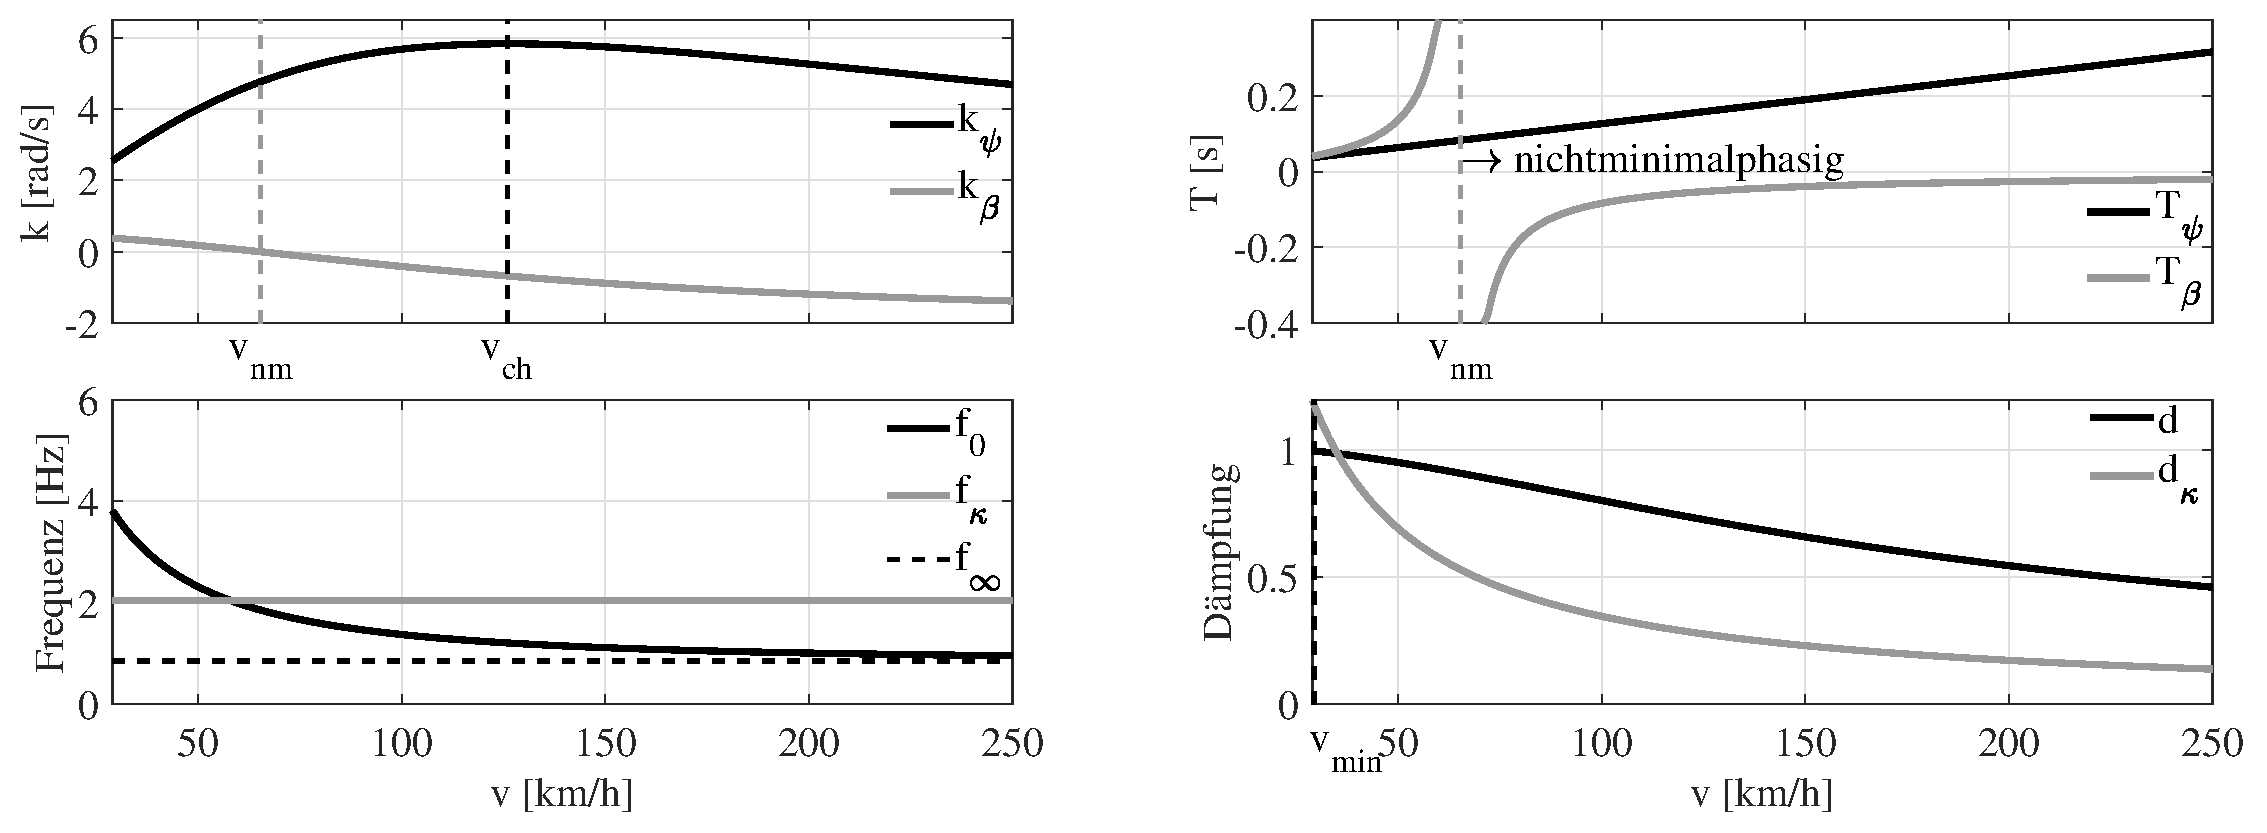
\includegraphics[width=12cm]{Bilder/ESM/esm_erg.eps} 
%	   \includegraphics[scale=1]{Bilder/ESM/esm.eps} 
%		\input{Bilder/ESM/esm.tex}
      \begin{center}
       \caption{Kenngrößen des dynamischen Übertragungsverhaltens}
     		 \label{fig:esm}
       \end{center}
\end{figure}      
Der Grenzwert $\omega_\infty=\lim_{v\to\infty} \omega(v)= (c_r \ell_r -c_f \ell_v)/i_z=2\pi f_\infty$ beschreibt die Bandbreite der Quer- und Gierdynamik für hohe Fahrgeschwindigkeiten. 
%Für große Geschwindigkeiten ist also die Schwerpunktlage, die über Reifen und Achskinematik definierte Balance  als Verhältnis der %Schräglaufsteifigkeiten und das Gierträgheitsmoment für die Bandbreite der Quer- und Gierdynamik bestimmend.  
Es ist leicht zu sehen, daß der Grenzwert der Bandbreite $\lim_{v\to 0} \omega(v)$ gegen $\infty$ geht. Weiterhin wird für $v=v_{\rm lim}$ die Dämpfung $d=1$ (aperiodischer Grenzfall), d.~h. für $v<v_{\rm lim}$ (ca. 20-30km/h) werden die Pole der Übertragungsfunktionen reell und der langsamere Pol der näher am Ursprung liegt wäre dominant und würde das Übertragungsverhalten dominieren. In Fahrversuchen hat sich jedoch gezeigt, dass für niedrige Geschwindigkeiten $v<v_{\rm lim}$ nichtmodellierte Dynamiken eine größere Rolle spielen und    
das vereinfachte lineare Einspurmodell 2. Ordnung nicht geeignet ist, diese Effekte abzubilden. Entsprechende Erweiterungen oder Vereinfachungen müssen für den Niedriggeschwindigkeitsbereich vorgenommen werden, auf die jedoch an dieser Stelle nicht weiter eingegangen werden soll.
Weitere Kenngrößen sind die charakteristische Fahrgeschwindigkeit die sehr gut das stationäre Gierübertragungsverhalten beschreibt. Für $v=v_{ch}$ wird die stationäre Gierverstärkung maximal, d.~h. die Gierempfindlichkeit des Fahrzeugs für diese Fahrgeschwindigkeit ist maximal. Die Geschwindigkeit $v_{nm}$ beschreibt die Fahrgeschwindigkeit oberhalb derer das Schwimmwinkelübertragungsverhalten nichtminimalphasig wird, d.~h. die Nullstellen dieser Übertragungsfunktion wandern im Eigenwertbereich in die rechte Halbebene. Während des Übergangs wechselt gleichzeitig die Schwimmwinkelverstärkung ihr Vorzeichen. Die langsamen Nullstellen haben wegen der geringen Verstärkung in diesem Geschwindigkeitsbereich $v\approx v_{nm}$ keinen bzw. wenig Einfluss auf das Übertragungsverhalten.    

Die Fahrzeugparameter und charakteristischen Kenngrößen des Einspurmodells und damit das Übertragungsverhalten hängen wesentlich von der Fahrzeuggeschwindigkeit, der Fahrzeugbeladung und dem reibwertabhängigen Reifen-Fahrbahnkontakt und damit vom Straßenzustand und der Bereifung ab.
Zusatzbeladung, Reifen und witterungsbedingter Reibwert bewirken Änderungen der Größen $m = m(m_{zus})$, $i_z(m_{zus})$, $l_f(m_{zus})$, $l_r(m_{zus})$, $c_f(m_{zus},\mu)$, $c_r(m_{zus},\mu)$. Für den regelungstechnischen Entwurf ist es notwendig, sich an die mess-, schätz- oder beobachtbaren variierenden Parameter zu adaptieren und entsprechend robust gegenüber nicht mess-, schätz- oder beobachtbaren variierenden Parametern zu sein. Eine Adaption der Reglerfunktionen an die Fahrgeschwindigkeit - ein variierender aber bekannter Parameter des Einspurmodells und gleichzeitig ein beobachteter Fahrzustand - über klassisches \textit{gainscheduling} ist Standard. Eine Adaption an eine veränderliche Zusatzbeladung mit ihrem Einfluss auf mehrere Fahrzeugparameter ist deutlich schwieriger. Das wird dann häufiger erst durch robuste Regleransätze beherrscht. 
Mit dem Betriebsbereich definiert durch die beladungsabhängige Schwerpunktlage, Masse und die variierende Fahrgeschwindigkeit $v\in[v^-, v^+]$, $R_1: m_{R1}$... ................. 

Die Identifikation des Einspurmodells erfolgt im Fahrversuch anhand von bidirektionalen Lenkwinkelsprüngen mit konstanter Querbeschleunigung über den gesamten Geschwindigkeitsbereich. Dieser Vorgang wiederholt für unterschiedliche Zusatzbeladungen und Bereifungen kann als Grundlage für die Bedatung der Parameter des Einspurmodells und für eine Beschreibung der zu betrachtenden Unsicherheiten dienen. 
\begin{figure}[thpb]
 	 \centering
	   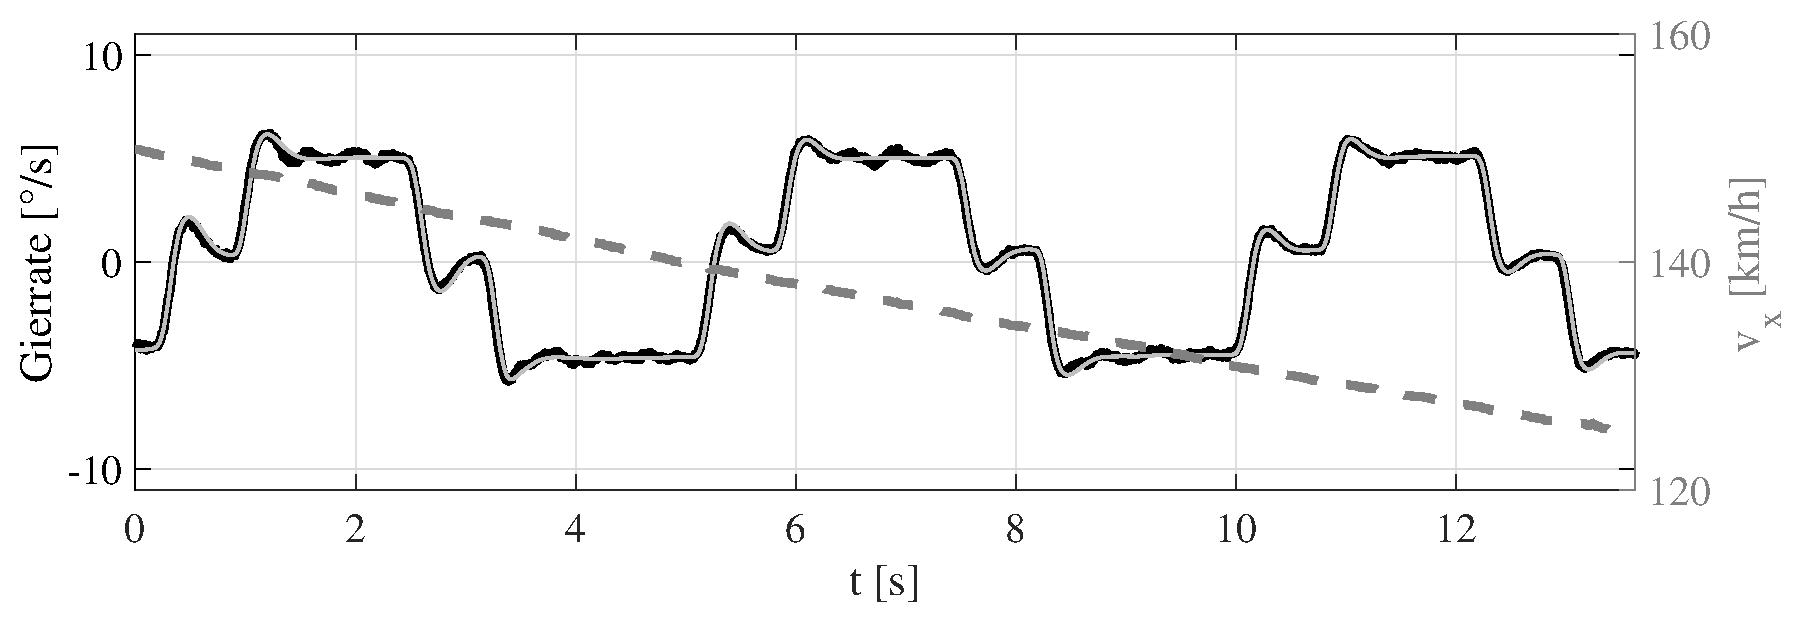
\includegraphics[width=12cm]{Bilder/ESM/esm_bidi_erg.eps} 
      \begin{center}
       \caption{Vergleich zwischen Einspurmodell- und gemessener Gierrate bei bidirektionalen Lenkwinkelsprüngen bei Fahrzeuggeschwindigkeiten zwischen 150 und 120 km/h}
     		 \label{abb_ident_esm}
       \end{center}
\end{figure}      


\subsection{Längsdynamik}
Zur Ansteuerung des Antriebs und der Bremse hat sich in heutigen Fahrzeug-Architekturen die Schnittstelle der Summen-Radmomente durchgesetzt.  Dies ist für die meisten Fahrerassistenzfunktionen ausreichend da keine Einzelradmomente zur Stabilisierung gestellt werden müssen und bietet den Vorteil, dass da so beide Aktuatoren, Antrieb und Bremse,  über die gleiche physikalische Größe angesteuert werden können.  Im Verlauf des Kapitels wird das Übertragungsverhalten vom Sollantriebsmoment $\tau_\mathrm{mot,d}$ bzw. Sollbremsmoment $\tau_\mathrm{brk,d}$ zum gemessen Radmoment $\tau_{xd}$ als System zweiter Ordnung mit Totzeit modelliert:
\begin{equation}
G_{\tau_x}^*(s)=\underbrace{\frac{k\omega_0^2}{s^2+2D\omega_0 s + \omega_0^2}}_{\displaystyle{G_{\tau_x}}}\;\mathrm{e}^{-T_\mathrm{D}s}\label{eq:GLong}
\end{equation}
Wie beim Lenkungsmodell 2 erfolgt die Identifikation im Fahrversuch anhand von Sollradmomentensprüngen bei verschiedenen Fahrzeuggeschwindigkeiten.  Abb.  \ref{abb_ident_antrieb_bremse} veranschaulicht die gute Übereinstimmung zwischen gemessenem und modelliertem Verhalten.
   \begin{figure}[thpb]
      \centering
	\setlength\figureheight{7cm} 
	\setlength\figurewidth{10.5cm}
    % This file was created by matlab2tikz v0.5.0 running on MATLAB 7.11.1.
%Copyright (c) 2008--2014, Nico Schlömer <nico.schloemer@gmail.com>
%All rights reserved.
%Minimal pgfplots version: 1.3
%
%The latest updates can be retrieved from
%  http://www.mathworks.com/matlabcentral/fileexchange/22022-matlab2tikz
%where you can also make suggestions and rate matlab2tikz.
%
\begin{tikzpicture}



\begin{axis}[%
 /pgf/number format/.cd,
        use comma,
        1000 sep={},
width=0.4\figurewidth,
height=0.383142\figureheight,
at={(0.010779\figurewidth,0\figureheight)},
scale only axis,
separate axis lines,
every outer x axis line/.append style={black},
every x tick label/.append style={font=\color{black}},
xmin=50,
xmax=73,
xlabel={$t$ [s]},
every outer y axis line/.append style={black},
every y tick label/.append style={font=\color{black}},
ymin=-500,
ymax=1500,
ylabel={$\tau_\mathrm{mot}$ [Nm]},
ylabel near ticks
]
\addplot [color=black , dashed, line width=1.0]
  table[row sep=crcr]{%
27.975	0\\
28.395	0\\
28.515	0\\
28.516	200\\
28.735	200\\
37.415	200\\
37.475	500\\
45.195	500\\
45.415	500\\
45.435	0\\
45.535	0\\
52.475	0\\
52.555	750\\
52.655	750\\
58.235	750\\
58.255	0\\
58.355	0\\
64.675	0\\
64.795	0\\
64.895	0\\
64.935	1000\\
69.815	1000\\
69.875	0\\
72.975	0\\
};


\addplot [color=light-gray,solid,line width=1.0]
  table[row sep=crcr]{%
27.975	-14.9009689478901\\
27.995	-8.62108796826086\\
28.015	-3.59000534065733\\
28.035	-6.83712520027438\\
28.055	-7.36166933699522\\
28.075	-4.51262684061924\\
28.095	-13.1582665751122\\
28.115	-10.2533150225068\\
28.135	-6.36714732585603\\
28.155	-0.472037842373989\\
28.175	-5.06512550545481\\
28.195	-0.502677958342659\\
28.215	-1.93250934615062\\
28.235	2.46086823834618\\
28.255	7.71827267872149\\
28.275	9.10684367132084\\
28.295	5.73459983215099\\
28.315	0.29079118028554\\
28.335	-2.60085450522602\\
28.355	-3.08279545281128\\
28.375	-0.943358510719309\\
28.395	6.65319295033199\\
28.415	9.92826733806377\\
28.435	-0.389517051956769\\
28.455	2.13334859235542\\
28.475	6.15928892957982\\
28.495	8.25612268253621\\
28.515	7.91663996337854\\
28.535	8.11500724803559\\
28.555	8.31337453269264\\
28.575	3.39679560540197\\
28.595	-0.261707484550028\\
28.615	-3.16665903715547\\
28.635	0.70351720454746\\
28.655	5.45102616922278\\
28.675	5.32321660181604\\
28.695	2.00688181887565\\
28.715	4.62825970855288\\
28.735	10.4528114747846\\
28.755	2.91485465781671\\
28.775	6.76903944457182\\
28.795	4.45918974593753\\
28.815	0.378683146410641\\
28.835	7.36414129854297\\
28.855	9.10684367132084\\
28.875	10.4528114747846\\
28.895	14.6185244525827\\
28.915	26.3221942473486\\
28.935	40.2079041733421\\
28.955	45.2522926680395\\
28.975	57.0878004119931\\
28.995	79.2996871900507\\
29.015	80.1224536507206\\
29.035	97.6387121385513\\
29.055	104.781277180132\\
29.075	103.392706187533\\
29.095	116.683314259555\\
29.115	127.015747310596\\
29.135	125.159884031433\\
29.155	144.334981307697\\
29.175	150.443106736857\\
29.195	151.249881742579\\
29.215	149.066498817425\\
29.235	153.234897383077\\
29.255	165.026459143968\\
29.275	168.172381170366\\
29.295	174.593377584496\\
29.315	167.918104829479\\
29.335	156.167803463797\\
29.355	162.829770351719\\
29.375	157.898542763408\\
29.395	165.749370565346\\
29.415	172.083817807277\\
29.435	167.818249790187\\
29.455	164.672327763789\\
29.475	173.203463797969\\
29.495	179.849439230944\\
29.515	172.890592812999\\
29.535	170.86565957122\\
29.555	175.11657892729\\
29.575	171.388860914014\\
29.595	164.147783627068\\
29.615	157.600320439459\\
29.635	160.647730220492\\
29.655	164.516563668268\\
29.675	168.470603494315\\
29.695	165.565651941709\\
29.715	167.534676127259\\
29.735	168.641016250857\\
29.755	173.204806591896\\
29.775	175.031372549018\\
29.795	192.05238422217\\
29.815	196.051712825207\\
29.835	173.857160296024\\
29.855	183.650400549324\\
29.875	194.093308918897\\
29.895	186.354299229418\\
29.915	194.786923018233\\
29.935	185.164095521476\\
29.955	180.85592431525\\
29.975	205.898176546882\\
29.995	202.836118104828\\
30.015	199.221560997939\\
30.035	206.989868009459\\
30.055	195.68158999008\\
30.075	198.430777447164\\
30.095	205.345677882046\\
30.115	202.22905317769\\
30.135	230.261463340198\\
30.155	216.696559090561\\
30.175	200.044327458608\\
30.195	224.322407873654\\
30.215	202.49663538567\\
30.235	196.754604409856\\
30.255	199.30676737621\\
30.275	173.641458762492\\
30.295	170.610040436407\\
30.315	185.222690165559\\
30.335	179.071961547264\\
30.355	173.813214312961\\
30.375	170.398367284656\\
30.395	176.123064011596\\
30.415	169.093659876401\\
30.435	177.879072251467\\
30.455	190.802243076217\\
30.475	182.328358892194\\
30.495	211.961013199052\\
30.515	220.080766002897\\
30.535	185.17740138857\\
30.555	213.550637064163\\
30.575	231.350469214922\\
30.595	221.912703135727\\
30.615	221.004730296786\\
30.635	208.689967193101\\
30.655	210.616388189515\\
30.675	200.044327458608\\
30.695	181.2952620737\\
30.715	207.823254749369\\
30.735	211.493720912488\\
30.755	205.867536430913\\
30.775	203.897169451437\\
30.795	201.206576638436\\
30.815	223.298588540473\\
30.835	223.089600976576\\
30.855	198.758297093155\\
30.875	209.155916685739\\
30.895	211.650827801936\\
30.915	198.131212329288\\
30.935	192.461081864651\\
30.955	208.60476081483\\
30.975	206.678339818416\\
30.995	184.937773708704\\
31.015	202.340871290149\\
31.035	206.183093003737\\
31.055	207.626230258639\\
31.075	224.093400473028\\
31.095	204.950286106659\\
31.115	194.121263447012\\
31.135	207.598275730524\\
31.155	199.406622415502\\
31.175	198.99389639124\\
31.195	203.147646295871\\
31.215	202.014694438085\\
31.235	194.502006561378\\
31.255	201.134676127259\\
31.275	204.947600518805\\
31.295	210.672297245745\\
31.315	211.15423819333\\
31.335	204.196734569313\\
31.355	209.185214007781\\
31.375	213.947371633477\\
31.395	205.145967803462\\
31.415	204.478965438314\\
31.435	206.334828717478\\
31.455	197.888899061569\\
31.475	198.613153276873\\
31.495	203.331364919507\\
31.515	208.361104753184\\
31.535	199.533089188981\\
31.555	203.304753185319\\
31.575	213.308323796443\\
31.595	207.90846112764\\
31.615	205.840924696725\\
31.635	202.551201647973\\
31.655	187.302189669641\\
31.675	184.001846341648\\
31.695	191.852674143586\\
31.715	203.047791256579\\
31.735	195.36871900511\\
31.755	204.521568627449\\
31.775	202.5525444419\\
31.795	203.742748149842\\
31.815	214.654291599907\\
31.835	215.406500343326\\
31.855	215.548958571754\\
31.875	202.837460898755\\
31.895	192.208148317691\\
31.915	200.128191042953\\
31.935	203.657541771571\\
31.955	187.388738841839\\
31.975	186.990661478598\\
31.995	198.075303273059\\
32.015	204.509605554283\\
32.035	218.057175555045\\
32.055	224.080094605934\\
32.075	216.442282749674\\
32.095	225.612466620888\\
32.115	225.372838941022\\
32.135	209.343663691156\\
32.155	204.947600518805\\
32.175	197.77708094911\\
32.195	192.462424658578\\
32.215	188.534996566719\\
32.235	193.681925688562\\
32.255	196.432455939573\\
32.275	205.786358434423\\
32.295	207.853894865338\\
32.315	213.763653009841\\
32.335	220.309773403523\\
32.355	212.544151979857\\
32.375	209.386266880292\\
32.395	201.277134355686\\
32.415	193.413000686655\\
32.435	197.098115510794\\
32.455	188.977019913022\\
32.475	194.149217975126\\
32.495	205.176607919431\\
32.535	207.061768520636\\
32.555	218.909239337757\\
32.575	214.614373998625\\
32.595	210.773495078964\\
32.615	215.351934081024\\
32.635	211.339299610893\\
32.655	219.17547875181\\
32.675	216.042862592506\\
32.695	214.940550850689\\
32.715	213.707743953611\\
32.735	203.886549172197\\
32.755	204.324544136719\\
32.775	216.796414129853\\
32.795	214.401358052947\\
32.815	218.015915159837\\
32.835	224.038834210725\\
32.875	222.381338216219\\
32.895	215.406500343326\\
32.915	208.406393530173\\
32.935	204.296589608605\\
32.955	193.934859235522\\
32.975	201.334386205843\\
32.995	213.494728007933\\
33.015	212.17402914473\\
33.035	205.018158236056\\
33.055	218.666926070037\\
33.075	225.199740596626\\
33.095	209.921431296252\\
33.115	221.248386358433\\
33.135	215.734019989317\\
33.155	195.254215304798\\
33.175	206.622430762187\\
33.215	198.75158312352\\
33.235	207.144289311054\\
33.255	208.588769359882\\
33.275	205.639871824214\\
33.295	213.606546120392\\
33.315	221.969954985884\\
33.335	208.008316166932\\
33.355	210.416678110931\\
33.375	225.230380712595\\
33.395	205.344335088119\\
33.415	209.623208972303\\
33.435	217.350255588615\\
33.455	200.582177462423\\
33.475	195.975783932248\\
33.495	209.102693217363\\
33.515	209.454139009688\\
33.535	210.472587167161\\
33.555	212.401693751429\\
33.575	214.865964751658\\
33.595	216.68191042954\\
33.615	212.614709697107\\
33.635	204.665369649804\\
33.655	194.587212939649\\
33.675	202.071946288241\\
33.695	205.658548867016\\
33.715	196.487022201875\\
33.735	202.864072632943\\
33.755	209.030792706186\\
33.775	210.616388189515\\
33.795	211.35126268406\\
33.815	222.081773098343\\
33.835	224.661890592811\\
33.855	211.875806820781\\
33.875	202.893369954984\\
33.895	207.31738765545\\
33.915	219.942336156251\\
33.935	201.900190737772\\
33.955	205.205905241473\\
33.975	197.394995040816\\
33.995	203.488471808956\\
34.015	218.115770199129\\
34.035	209.783001449606\\
34.055	215.77796597238\\
34.075	240.40749217975\\
34.095	232.641870756083\\
34.115	230.602288853283\\
34.135	235.717235065231\\
34.155	219.914381628136\\
34.175	218.002609292743\\
34.195	202.894712748911\\
34.215	206.491935606926\\
34.235	209.837567711908\\
34.255	194.517998016326\\
34.275	203.475165941862\\
34.295	213.381567101547\\
34.315	213.74900434882\\
34.335	219.247379262988\\
34.355	222.495841916532\\
34.375	214.517204547187\\
34.395	212.190020599678\\
34.415	203.31940184634\\
34.435	193.00161745632\\
34.455	212.090165560386\\
34.475	205.757061112381\\
34.495	192.292011902036\\
34.515	209.171908140687\\
34.535	208.619409475851\\
34.555	204.564171816585\\
34.575	232.442160677499\\
34.595	221.871442740519\\
34.615	222.182970931562\\
34.635	227.624093995573\\
34.655	202.371511406118\\
34.675	217.805584802013\\
34.695	226.887876707101\\
34.715	211.540352483404\\
34.735	223.699351491568\\
34.755	221.004730296786\\
34.775	226.786678873882\\
34.795	223.741954680703\\
34.815	208.832425421529\\
34.835	214.473258564125\\
34.855	214.277576867321\\
34.875	210.17973601892\\
34.895	209.625894560157\\
34.915	205.473487449453\\
34.935	207.088380254824\\
34.955	200.245380331119\\
34.975	194.420828564888\\
34.995	201.744426642251\\
35.015	206.763546196687\\
35.035	202.866758220797\\
35.055	208.944243533988\\
35.075	215.77796597238\\
35.095	212.348470283053\\
35.115	205.445532921338\\
35.135	207.289433127335\\
35.155	212.659998474096\\
35.175	218.965148393986\\
35.195	211.992996108948\\
35.215	212.120805676355\\
35.235	217.802899214159\\
35.255	218.895933470663\\
35.275	214.983154039825\\
35.295	227.058289463644\\
35.315	221.079316395818\\
35.335	220.31111619745\\
35.355	223.642099641411\\
35.375	211.087708857861\\
35.395	207.330693522544\\
35.415	207.684824902722\\
35.435	198.489372091248\\
35.455	198.899412527656\\
35.475	204.184771496146\\
35.495	204.284626535438\\
35.515	205.446875715265\\
35.535	205.106050202181\\
35.555	202.937315938047\\
35.575	209.953414206148\\
35.595	210.223682001982\\
35.615	219.464423590446\\
35.635	217.692423895627\\
35.655	199.09912260624\\
35.675	205.828961623559\\
35.695	210.279591058212\\
35.715	208.366475928892\\
35.735	207.626230258639\\
35.755	205.16195925841\\
35.775	213.396215762568\\
35.795	221.119233997099\\
35.815	218.794735637444\\
35.835	227.287296864269\\
35.855	218.286182955671\\
35.875	207.073731593803\\
35.895	203.263492790111\\
35.915	207.445197222857\\
35.935	190.251087205309\\
35.955	189.472266727701\\
35.975	201.334386205843\\
35.995	193.154695963987\\
36.015	201.98673990997\\
36.035	224.707179369801\\
36.055	217.801556420232\\
36.075	223.840466926068\\
36.095	220.413656824596\\
36.115	220.934172579536\\
36.135	227.083558403905\\
36.155	215.055054551002\\
36.175	216.343770504309\\
36.195	219.03436331731\\
36.215	204.341878385594\\
36.235	211.640207522696\\
36.255	222.352040894177\\
36.275	224.536766613259\\
36.295	223.982925154496\\
36.315	220.976775768672\\
36.335	226.533745326923\\
36.355	215.904432745859\\
36.375	201.349034866864\\
36.395	219.958327611199\\
36.415	216.79775692378\\
36.435	209.414221408406\\
36.455	216.767116807811\\
36.475	213.919417105362\\
36.495	212.02229343099\\
36.515	207.285404745554\\
36.535	213.947371633477\\
36.555	226.577691309985\\
36.575	219.292668039977\\
36.595	212.674647135117\\
36.615	220.35640497444\\
36.635	214.952513923856\\
36.655	209.7963073167\\
36.675	204.227374685281\\
36.695	205.755718318454\\
36.715	210.844052796214\\
36.735	211.384588387883\\
36.755	219.630807965208\\
36.775	227.168764782176\\
36.795	229.6650186923\\
36.815	231.394415197984\\
36.835	225.866742961774\\
36.855	218.965148393986\\
36.875	216.427634088653\\
36.895	218.865293354694\\
36.915	210.915953307391\\
36.935	215.917738612953\\
36.955	217.532631418324\\
36.975	210.37676050965\\
36.995	208.391744869152\\
37.015	212.940886549171\\
37.035	218.270191500723\\
37.055	227.327214465551\\
37.075	220.142046234835\\
37.095	214.573113603417\\
37.115	219.491035324634\\
37.135	217.62052338445\\
37.155	213.382909895474\\
37.175	211.710765239947\\
37.195	213.368261234453\\
37.215	217.293003738459\\
37.235	219.278019378956\\
37.255	225.656412603951\\
37.295	219.577584496832\\
37.315	210.846738384068\\
37.335	201.238559548332\\
37.355	197.850324254214\\
37.375	206.014023041122\\
37.395	200.38649576562\\
37.415	206.168444342716\\
37.435	206.534538796062\\
37.455	207.27209887846\\
37.475	211.325993743799\\
37.495	213.791607537955\\
37.515	219.29132524605\\
37.535	222.694209201189\\
37.555	217.917402914472\\
37.575	210.645685511557\\
37.595	196.516319523917\\
37.615	191.979140917066\\
37.635	195.991775387196\\
37.655	205.614602883954\\
37.675	205.201876859692\\
37.695	206.903318837261\\
37.715	215.507698176545\\
37.735	224.974761577781\\
37.755	253.928450446325\\
37.775	278.756343938351\\
37.795	288.705348287173\\
37.815	288.038345922024\\
37.835	289.187289234758\\
37.855	300.978850995649\\
37.875	306.575738155182\\
37.895	299.218814373996\\
37.915	302.47789730678\\
37.935	305.412146181427\\
37.955	306.702204928662\\
37.975	309.637796597236\\
37.995	316.808316166931\\
38.015	327.665293354694\\
38.035	347.096009765771\\
38.055	350.353749904628\\
38.075	348.158403906307\\
38.095	344.089860379947\\
38.115	339.579293507283\\
38.135	350.890257114516\\
38.155	354.237232013425\\
38.175	363.037293049513\\
38.195	381.689188982983\\
38.215	382.228381780725\\
38.235	398.708857862208\\
38.255	415.886976424808\\
38.275	408.572655832758\\
38.295	400.663233386737\\
38.315	394.358083466847\\
38.335	408.328999771111\\
38.355	410.866514076444\\
38.375	408.810940718697\\
38.395	425.148958571752\\
38.415	438.018905928126\\
38.435	432.320820935375\\
38.455	442.836972610052\\
38.475	458.752986953533\\
38.495	466.461356527043\\
38.515	475.674143587392\\
38.535	474.201709010449\\
38.555	474.526543068586\\
38.575	468.984222171355\\
38.595	470.330189974819\\
38.615	477.585915922785\\
38.635	481.087312123289\\
38.655	479.783947508961\\
38.675	474.199023422595\\
38.695	479.967666132597\\
38.715	481.55594720378\\
38.735	479.175539787896\\
38.755	476.9628595407\\
38.775	463.029175249863\\
38.795	453.267917906459\\
38.815	469.19858091096\\
38.835	488.4269016556\\
38.855	473.402868696113\\
38.875	468.129472800789\\
38.895	466.995178149077\\
38.915	473.259067673758\\
38.935	480.501487754631\\
38.955	479.553597314408\\
38.975	489.574502174407\\
38.995	490.736751354234\\
39.015	487.762584878305\\
39.035	490.454520485233\\
39.055	497.085847257187\\
39.075	494.520378423739\\
39.095	491.630075532154\\
39.115	493.499244678412\\
39.135	480.28981460288\\
39.155	490.324025329972\\
39.175	502.967650873575\\
39.195	496.095353627828\\
39.215	495.911635004192\\
39.235	497.554482337678\\
39.255	503.205935759514\\
39.275	507.797680628667\\
39.295	498.076340886545\\
39.315	505.17630273899\\
39.335	507.233218890665\\
39.355	519.959365224685\\
39.375	520.752834363313\\
39.395	500.476768139158\\
39.415	518.998168917368\\
39.435	502.47508964675\\
39.455	500.150591287095\\
39.475	509.094453345537\\
39.495	501.625711451892\\
39.515	506.314625772484\\
39.535	505.406652933543\\
39.555	501.194308384828\\
39.575	505.093781948573\\
39.595	520.242938887613\\
39.615	525.854474708167\\
39.635	518.004989700156\\
39.655	509.443213550007\\
39.675	501.423315785454\\
39.695	512.081925688559\\
39.715	508.906706340119\\
39.735	513.909834439608\\
39.755	518.586785687033\\
39.775	514.307911802849\\
39.795	514.535576409548\\
39.815	518.122178988323\\
39.835	525.90244907301\\
39.855	521.877851529713\\
39.875	526.638666361482\\
39.895	520.161760891123\\
39.915	512.478660257873\\
39.935	507.984084840158\\
39.955	506.795223926142\\
39.975	517.365941863122\\
39.995	517.138277256424\\
40.015	522.724544136717\\
40.035	520.442648966197\\
40.055	521.507728694587\\
40.075	526.227283131147\\
40.095	521.419836728461\\
40.115	526.906248569462\\
40.135	524.552452887766\\
40.155	502.444449530781\\
40.175	519.208499275192\\
40.195	526.192614633398\\
40.215	519.520027466235\\
40.235	527.368169680319\\
40.255	518.753170061795\\
40.275	527.248416876474\\
40.295	529.14419775692\\
40.315	524.352742809182\\
40.335	515.78168917372\\
40.355	513.770061799035\\
40.375	517.781353475238\\
40.395	521.662149996181\\
40.415	528.734157320511\\
40.435	529.216098268097\\
40.455	523.078675516895\\
40.475	524.953215838861\\
40.495	514.381155107954\\
40.515	526.309803921564\\
40.535	523.150576028072\\
40.555	507.150698100248\\
40.575	509.375341420611\\
40.595	515.143984130613\\
40.615	527.827527275497\\
40.635	523.022766460666\\
40.655	517.242160677496\\
40.675	519.894178683142\\
40.695	519.767711909663\\
40.715	506.644831006329\\
40.735	509.436621652548\\
40.755	518.775875486377\\
40.775	512.073990997173\\
40.795	514.029709315629\\
40.815	518.706660563054\\
40.835	521.624917982753\\
40.855	524.174395361253\\
40.875	527.179201953151\\
40.895	543.602426184477\\
40.915	537.989547569996\\
40.935	530.207934691382\\
40.955	518.798458838784\\
40.975	510.115587090864\\
40.995	516.904020752266\\
41.015	536.377340352479\\
41.035	540.572350652319\\
41.055	550.886106660559\\
41.075	545.99882505531\\
41.095	537.496986343171\\
41.115	529.956343938349\\
41.135	526.785152971691\\
41.155	527.067383840692\\
41.175	524.925261310746\\
41.195	517.725444419009\\
41.215	523.207827878229\\
41.235	523.054749370561\\
41.255	523.705760280762\\
41.275	522.245288776985\\
41.295	535.041992828256\\
41.315	538.456839856561\\
41.335	542.014145113294\\
41.355	541.68796826123\\
41.375	523.660471503772\\
41.395	518.403067063397\\
41.415	513.908491645681\\
41.435	518.171374074917\\
41.455	527.228397039745\\
41.475	520.582421606771\\
41.495	517.324681467914\\
41.515	521.391882200347\\
41.535	518.340444037533\\
41.555	509.56833752956\\
41.575	503.826306553746\\
41.595	504.153826199736\\
41.615	519.87147325856\\
41.635	522.523491264206\\
41.655	522.739192797737\\
41.675	530.858945601583\\
41.695	544.618188754096\\
41.715	539.700267032879\\
41.735	528.913847562367\\
41.755	524.307454032192\\
41.775	520.88064393072\\
41.795	520.272236209655\\
41.815	517.123628595403\\
41.835	513.240146486606\\
41.855	522.619317921717\\
41.875	517.942366674292\\
41.895	518.213977264053\\
41.915	520.651636530094\\
41.935	515.098695353624\\
41.955	500.869474326691\\
41.975	502.50035858701\\
41.995	513.11636530098\\
42.015	509.074433508808\\
42.035	514.049607080182\\
42.055	522.542168307007\\
42.075	529.615518425265\\
42.095	526.002304112302\\
42.115	517.396581979091\\
42.135	503.733165484088\\
42.175	500.106645304032\\
42.195	494.987670710303\\
42.215	489.75956359197\\
42.235	513.919111924921\\
42.255	519.176516365296\\
42.275	510.65868619821\\
42.295	523.994583047222\\
42.315	526.09947356374\\
42.335	499.752513923853\\
42.355	493.798809796288\\
42.375	504.26173800259\\
42.395	499.185366597997\\
42.415	524.133134966045\\
42.435	531.970656900889\\
42.455	533.96897840848\\
42.475	515.20526436255\\
42.495	502.29271381704\\
42.515	502.021103227279\\
42.535	489.919356069272\\
42.555	501.467261768517\\
42.575	504.71169604028\\
42.595	514.547539482715\\
42.615	525.260715648123\\
42.635	534.275135423815\\
42.655	530.351735713737\\
42.675	531.017395284958\\
42.695	515.102723735404\\
42.715	509.304783703361\\
42.735	501.77878995956\\
42.755	502.544304570073\\
42.775	507.575387197677\\
42.795	511.741100175475\\
42.815	522.34380102235\\
42.835	523.238467994197\\
42.855	525.37790493629\\
42.875	520.091203173872\\
42.895	511.745128557256\\
42.915	487.509651331346\\
42.935	488.384298466464\\
42.955	500.221149004345\\
42.975	507.177309834435\\
42.995	512.495994506748\\
43.015	526.216662851907\\
43.035	510.010360875864\\
43.055	505.663614862283\\
43.075	496.406881818871\\
43.095	492.933440146483\\
43.115	502.529655909052\\
43.135	508.279621576253\\
43.155	513.047150377657\\
43.175	516.109208819711\\
43.195	527.073975738151\\
43.215	511.418951705192\\
43.235	508.613855191878\\
43.255	509.280857557027\\
43.275	494.388662546727\\
43.295	490.236255436023\\
43.315	499.942946517124\\
43.335	502.874509803918\\
43.355	514.153490501255\\
43.375	511.277836270691\\
43.395	509.263523308152\\
43.415	511.317753871973\\
43.435	496.934111543446\\
43.455	500.545983062482\\
43.475	512.902006561375\\
43.495	507.562081330583\\
43.515	500.942717631796\\
43.535	504.257709620809\\
43.555	508.665735866327\\
43.575	507.756420233459\\
43.595	504.027359426256\\
43.615	491.4862745098\\
43.635	494.391226062405\\
43.655	507.515449759666\\
43.675	520.169695582509\\
43.695	527.878065156019\\
43.715	519.802258335236\\
43.735	525.670756084531\\
43.755	518.529533836877\\
43.775	511.13269245441\\
43.795	508.764248111692\\
43.815	501.905256733039\\
43.835	505.772747386888\\
43.855	516.263630121305\\
43.875	514.267994201568\\
43.895	520.629053177687\\
43.915	503.562752727546\\
43.935	499.804394598302\\
43.955	482.976501106275\\
43.975	481.557289997707\\
43.995	502.653437094678\\
44.015	504.428122377351\\
44.035	515.133363851373\\
44.055	518.052964065\\
44.075	519.582650492099\\
44.095	514.720637827111\\
44.115	508.356893263138\\
44.135	497.346837567708\\
44.155	491.891065842676\\
44.175	498.435843442431\\
44.195	508.496665903711\\
44.215	522.36504158083\\
44.235	517.843854428927\\
44.255	508.793545433734\\
44.275	503.612069886316\\
44.295	511.461554894327\\
44.315	511.831677729454\\
44.335	510.513664454105\\
44.355	497.754192416262\\
44.375	499.146791790642\\
44.395	499.901686121916\\
44.415	513.901899748222\\
44.435	527.529304951548\\
44.455	520.993804837106\\
44.475	502.873167009991\\
44.495	500.708461127638\\
44.515	503.750499732963\\
44.535	503.49488059815\\
44.555	511.235233081556\\
44.575	525.310032806893\\
44.595	515.431586175322\\
44.615	501.939925230789\\
44.635	495.818493934535\\
44.655	489.397497520405\\
44.675	465.167391470203\\
44.695	463.905287251084\\
44.715	482.622369726097\\
44.735	497.388097962917\\
44.755	505.694254978252\\
44.775	501.44467841611\\
44.795	490.24821850919\\
44.815	472.147478446628\\
44.835	476.727260242615\\
44.855	485.004119935908\\
44.875	475.108339055463\\
44.895	490.999084458682\\
44.915	503.10083161669\\
44.935	508.38619058518\\
44.955	489.607827878229\\
44.975	483.072327763786\\
44.995	486.360708018612\\
45.015	482.322804608221\\
45.035	487.633432516972\\
45.055	504.470725566487\\
45.075	514.037644007015\\
45.095	511.614633401995\\
45.115	506.327931639578\\
45.135	506.501029983974\\
45.155	505.153719386583\\
45.175	517.807965209426\\
45.195	524.282185091931\\
45.215	532.447226672766\\
45.235	525.558937972072\\
45.255	516.75619134813\\
45.275	513.059113450824\\
45.295	515.784374761574\\
45.315	502.391226062406\\
45.335	508.541954680701\\
45.355	514.097581445025\\
45.375	515.130678263519\\
45.395	518.871702143888\\
45.415	516.788174258026\\
45.435	509.139742122526\\
45.455	502.934447241928\\
45.475	495.21008621347\\
45.495	492.205279621573\\
45.515	500.253131914241\\
45.535	494.499137865259\\
45.555	510.938353551533\\
45.575	521.284092469669\\
45.595	507.126771953914\\
45.615	488.094132906077\\
45.635	459.013977264054\\
45.655	422.660761425189\\
45.675	363.335515373462\\
45.695	280.673487449453\\
45.715	198.050034332798\\
45.735	132.021560997939\\
45.755	79.2158236057065\\
45.775	50.4471961547263\\
45.795	54.1589227130539\\
45.815	57.9718471046004\\
45.835	71.0800793469135\\
45.855	95.5831387808036\\
45.875	105.88761730373\\
45.895	112.023697261005\\
45.915	114.036667429617\\
45.935	98.8449073014415\\
45.955	70.6274357213699\\
45.975	55.5754482337679\\
45.995	33.5393453879606\\
46.015	17.2971541924163\\
46.035	14.477409018082\\
46.055	13.6839398794538\\
46.075	12.1542534523539\\
46.095	10.6378728923478\\
46.115	4.51644159609396\\
46.135	13.4855725947968\\
46.155	8.72475776302759\\
46.175	8.44118410009938\\
46.195	14.1938353551538\\
46.215	10.6658274204625\\
46.235	8.52639047837054\\
46.255	8.28542000457791\\
46.275	7.69031815060676\\
46.295	8.04444953078528\\
46.315	8.32802319371349\\
46.355	11.6150606546122\\
46.375	8.37062638284907\\
46.415	3.56720836194429\\
46.435	8.32802319371349\\
46.455	10.8641947051196\\
46.475	8.44118410009938\\
46.495	6.25914396887183\\
46.535	6.93945220111414\\
46.555	8.24281681544233\\
46.575	5.86240939955773\\
46.595	6.14598306248594\\
46.615	4.36067750057249\\
46.635	-1.39197375448196\\
46.655	0.591699092088541\\
46.675	-1.63294422827459\\
46.695	7.53455405508529\\
46.715	7.25098039215708\\
46.735	-2.90835431448805\\
46.755	-17.3931944762336\\
46.775	-9.81263447013013\\
46.795	-12.9585564965282\\
46.815	-13.2141756313417\\
46.835	-16.74352635996\\
46.855	-23.7289845120923\\
46.875	-16.0618753337907\\
46.895	-6.14216830701122\\
46.915	-7.67185473411119\\
46.935	-3.71781490806407\\
46.955	-3.83231860837693\\
46.975	-4.66704814221374\\
46.995	-7.68516060120507\\
47.015	5.77451743343263\\
47.035	-3.79105821316832\\
47.055	1.42642862592535\\
47.075	-5.97041275654193\\
47.095	-1.03918516823041\\
47.115	-4.39946593423335\\
47.135	2.5140917067217\\
47.155	3.83210498207074\\
47.175	-2.14821087968246\\
47.195	-6.69735255970073\\
47.215	-1.29480430304389\\
47.235	1.96562142366704\\
47.255	-3.3490348668647\\
47.295	-11.045441367208\\
47.315	-2.26002899214138\\
47.335	3.12652780956764\\
47.355	5.94627298390192\\
47.375	6.63988708323811\\
47.395	4.50045014114614\\
47.415	1.80985732814557\\
47.435	5.1954070344093\\
47.455	2.14934004730324\\
47.475	4.62825970855288\\
47.495	3.74958419165352\\
47.515	8.66750591287116\\
47.535	1.84977492942721\\
47.555	11.4872510872054\\
47.575	12.1955138475625\\
47.595	8.51174181734969\\
47.615	8.90847638666379\\
47.635	8.45448996719326\\
47.655	13.5414816510263\\
47.675	9.74454871442757\\
47.695	11.8839856565195\\
47.715	15.7235217822538\\
47.735	12.5216906996263\\
47.755	10.0986800946061\\
47.775	12.8052643625545\\
47.795	11.1331197070269\\
47.815	8.24281681544233\\
47.835	6.52806897077919\\
47.855	1.05899137865295\\
47.875	6.4149080643933\\
47.895	17.325108720531\\
47.915	9.70194552529199\\
47.935	8.20021362630675\\
47.955	7.2083772030215\\
47.975	6.06077668421478\\
47.995	7.95924315251412\\
48.015	4.04780651560258\\
48.035	4.2182192721449\\
48.055	-0.531975280384358\\
48.075	-10.747219043259\\
48.095	-4.07194628824259\\
48.115	-21.1342183566028\\
48.135	-25.1748073548481\\
48.155	-43.087800411993\\
48.175	-51.1662928206295\\
48.195	-47.664896620126\\
48.215	-41.6859235522997\\
48.235	-27.3581902800026\\
48.255	-14.8437170977337\\
48.275	-5.53241779201922\\
48.295	2.60332646677377\\
48.315	-0.486686503394839\\
48.335	-7.60263981078785\\
48.355	-4.28630502784746\\
48.375	0.475852597848711\\
48.395	0.220233463035232\\
48.415	6.35765621423687\\
48.435	6.72643625543624\\
48.455	-0.586541542686849\\
48.475	2.48882276646091\\
48.495	6.03147936217308\\
48.515	-2.13221942473464\\
48.535	-0.74364843213529\\
48.555	7.71827267872149\\
48.575	5.84776073853688\\
48.595	5.97557030594362\\
48.615	9.46097505149936\\
48.635	7.23633173113623\\
48.655	2.47551689936703\\
48.675	5.8051575494013\\
48.695	4.27278553444739\\
48.715	1.75126268406217\\
48.735	5.93162432288107\\
48.755	4.33003738460382\\
48.775	-4.05998321507568\\
48.795	-0.24840161745615\\
48.815	5.20871290150318\\
48.835	2.9987182421609\\
48.855	-0.458731975280109\\
48.875	-3.010894941634\\
48.895	-2.06031891355736\\
48.915	2.77239642938912\\
48.935	0.362691691462821\\
48.955	1.01370260166343\\
48.975	6.34032196536208\\
48.995	9.90031280994904\\
49.015	8.38393224994295\\
49.035	4.45650415808359\\
49.055	2.41557946135666\\
49.095	5.63340199893201\\
49.115	4.41390096894801\\
49.135	8.96304264896628\\
49.155	3.63642328526763\\
49.175	5.86106660563076\\
49.195	9.07754634927914\\
49.215	4.65487144274064\\
49.235	2.3596704051272\\
49.255	-3.52079041733399\\
49.275	-1.19629205767885\\
49.295	1.11490043488241\\
49.315	-1.15368886854327\\
49.335	7.32153810940739\\
49.355	6.10203707942339\\
49.375	6.99401846341663\\
49.395	-0.318959334706459\\
49.415	-5.26483558403883\\
49.435	3.35284962233942\\
49.455	-1.84730296787946\\
49.475	0.19093614099353\\
49.495	6.89416342412462\\
49.515	5.52158388647309\\
49.535	-3.30643167772912\\
49.555	1.32791638056031\\
49.575	0.505149919890411\\
49.595	-12.0239719233994\\
49.615	0.80337224383947\\
49.635	5.12484931715899\\
49.655	3.02667277027563\\
49.675	6.34435034714299\\
49.695	2.89886320286889\\
49.715	5.29526207370131\\
49.735	7.67566948958591\\
49.755	8.11500724803559\\
49.775	5.08224612802341\\
49.795	4.03181506065476\\
49.815	6.42687113756021\\
49.835	11.9119401846343\\
49.855	9.3757686732282\\
49.875	6.88220035095771\\
49.895	5.33786526283689\\
49.915	3.90669108110196\\
49.935	7.12317082475034\\
49.955	7.32153810940739\\
49.975	6.64122987716508\\
49.995	9.81510643167788\\
50.015	8.11500724803559\\
50.035	14.4627603570612\\
50.055	15.2136263065538\\
50.075	11.1331197070269\\
50.095	13.2725566491189\\
50.115	13.9102616922256\\
50.135	11.331486991684\\
50.155	10.5380178530558\\
50.175	12.4790875104907\\
50.195	13.7118944075686\\
50.215	9.74454871442757\\
50.235	8.75271229114232\\
50.255	5.18210116731542\\
50.275	8.99368276493495\\
50.295	6.8116426337074\\
50.315	7.36414129854297\\
50.335	4.98373388265837\\
50.355	5.77720302128657\\
50.375	9.50357824063494\\
50.395	11.1757228961625\\
50.415	7.67566948958591\\
50.435	5.18210116731542\\
50.455	4.4312352178228\\
50.475	6.0181734950792\\
50.495	3.39679560540197\\
50.515	5.73459983215099\\
50.535	12.1249561303122\\
50.555	12.3233234149692\\
50.575	7.76087586785707\\
50.595	4.21687647821793\\
50.615	6.72643625543624\\
50.635	9.94291599908462\\
50.655	9.14944686045642\\
50.675	4.4312352178228\\
50.695	6.57067215991477\\
50.715	13.4283207446404\\
50.735	8.15761043717117\\
50.755	9.90031280994904\\
50.775	13.3151598382545\\
50.795	14.3495994506753\\
50.815	16.1349050125887\\
50.835	15.6955672541391\\
50.855	13.3577630273901\\
50.875	12.3659266041048\\
50.895	14.3922026398109\\
50.915	8.7953154802779\\
50.935	5.42307164110805\\
50.955	10.5806210421914\\
50.975	11.5724574654766\\
50.995	11.3740901808196\\
51.015	8.44118410009938\\
51.035	14.5905699244679\\
51.055	7.80347905699265\\
51.075	10.5806210421914\\
51.095	7.2083772030215\\
51.115	7.01000991836445\\
51.135	3.2410315098805\\
51.155	6.96740672922887\\
51.175	4.23286793316575\\
51.195	-3.54605935759478\\
51.215	1.45572594796705\\
51.235	-13.1995269703208\\
51.255	-8.91931029220992\\
51.275	1.18411535820575\\
51.295	1.02835126268428\\
51.315	-6.92233157854554\\
51.335	-3.26651407644748\\
51.355	-6.7945220111388\\
51.375	4.10505836575901\\
51.395	1.92301823453146\\
51.415	4.10505836575901\\
51.435	1.52494087129039\\
51.475	5.73459983215099\\
51.495	1.79386587319775\\
51.515	3.53656824597562\\
51.535	6.52806897077919\\
51.555	13.3151598382545\\
51.575	8.07240405890001\\
51.595	7.87403677424296\\
51.615	9.74454871442757\\
51.635	2.23320363164743\\
51.655	9.57413595788525\\
51.675	11.2462806134128\\
51.695	9.46097505149936\\
51.715	12.0823529411766\\
51.735	11.0479133287558\\
51.755	8.15761043717117\\
51.775	6.32970168612214\\
51.795	5.97557030594362\\
51.815	4.98373388265837\\
51.835	11.6856183718625\\
51.855	12.6774547951477\\
51.875	11.8839856565195\\
51.895	10.2970473792631\\
51.915	11.2462806134128\\
51.935	7.32153810940739\\
51.955	9.65934233615641\\
51.975	5.73459983215099\\
51.995	3.90669108110196\\
52.015	1.01370260166343\\
52.035	3.01336690318175\\
52.055	11.0905165178913\\
52.075	13.7118944075686\\
52.095	8.86587319752821\\
52.115	10.4528114747846\\
52.135	7.71827267872149\\
52.155	6.32970168612214\\
52.175	6.72643625543624\\
52.195	10.9347524223699\\
52.215	9.54618142977052\\
52.235	7.76087586785707\\
52.255	11.7708247501336\\
52.275	11.8839856565195\\
52.295	13.7118944075686\\
52.315	15.497199969482\\
52.335	18.8694438086519\\
52.355	14.9020981155109\\
52.375	13.159395742733\\
52.415	10.6937819485772\\
52.435	7.36414129854297\\
52.455	10.1412832837417\\
52.475	12.1249561303122\\
52.495	14.3495994506753\\
52.515	11.9691920347907\\
52.535	10.7789883268484\\
52.575	11.4166933699551\\
52.595	15.7807736324102\\
52.615	16.3332722972458\\
52.635	15.5398031586176\\
52.655	16.0923018234532\\
52.675	17.126741435874\\
52.695	17.9202105745022\\
52.715	19.7481193255512\\
52.735	41.9719691767757\\
52.755	44.2964675364308\\
52.775	56.5127183947507\\
52.795	64.8454871442738\\
52.815	72.7668726634619\\
52.835	82.7997405966273\\
52.855	94.8881818875404\\
52.875	112.348531319142\\
52.895	132.005569542991\\
52.915	137.7609063859\\
52.935	143.911635004195\\
52.955	162.815121690698\\
52.975	188.339314869915\\
52.995	210.829404135193\\
53.015	230.443839169908\\
53.035	264.47121385519\\
53.055	294.444693675133\\
53.075	334.905027847712\\
53.095	379.887891966122\\
53.115	417.76945143816\\
53.135	455.762829022656\\
53.155	493.290257114515\\
53.175	505.776775768669\\
53.195	522.528862439914\\
53.215	550.136583504993\\
53.235	561.587319752799\\
53.255	562.676325627523\\
53.275	580.051468680853\\
53.295	582.4758220798\\
53.315	566.758175020977\\
53.335	549.653299763481\\
53.355	531.399481193251\\
53.375	523.066712443728\\
53.395	527.501350423434\\
53.415	532.89987029831\\
53.435	541.855695429918\\
53.455	556.594811932551\\
53.475	574.379995422289\\
53.495	593.033234149686\\
53.515	607.629892423891\\
53.535	606.848386358429\\
53.555	603.761058976115\\
53.575	602.002365148389\\
53.595	618.128709849693\\
53.615	620.648889906152\\
53.635	600.708278019374\\
53.655	632.045059891656\\
53.675	660.361043717092\\
53.695	640.57888151369\\
53.715	640.791897459368\\
53.735	646.531242847328\\
53.755	642.621149004344\\
53.775	642.337575341415\\
53.795	653.56198977645\\
53.815	691.142641336685\\
53.835	678.12095826657\\
53.855	640.540306706335\\
53.875	665.910078583958\\
53.895	684.203814755469\\
53.915	672.751735713735\\
53.935	670.075791561756\\
53.955	697.454505226209\\
53.975	668.185259784842\\
53.995	637.430273899438\\
54.015	661.127901121533\\
54.035	687.546761272597\\
54.055	689.987106126492\\
54.075	695.060791943231\\
54.095	691.430243381394\\
54.115	679.853040360108\\
54.135	685.705546654454\\
54.155	705.787273975733\\
54.175	686.285999847404\\
54.195	664.066178377961\\
54.215	680.887479972528\\
54.235	684.572594796668\\
54.255	685.877302204923\\
54.275	709.941023880364\\
54.295	719.67566948958\\
54.315	698.102830548556\\
54.335	686.329945830467\\
54.355	687.988784618901\\
54.375	696.756862745092\\
54.395	721.158724345763\\
54.415	729.7471122301\\
54.435	718.819577325087\\
54.455	718.393545433732\\
54.475	729.05081254291\\
54.495	718.481437399857\\
54.515	723.469916838325\\
54.535	734.223010605014\\
54.555	716.380575265119\\
54.575	697.964400701909\\
54.595	700.046585793845\\
54.615	694.313832303343\\
54.635	706.741756313414\\
54.655	746.66826886396\\
54.675	749.674418249784\\
54.695	736.16810864423\\
54.715	739.581612878608\\
54.735	742.827389944298\\
54.755	754.00785839627\\
54.775	758.981689173718\\
54.795	747.387151903557\\
54.815	726.69835965514\\
54.835	719.483894102382\\
54.855	733.994003204388\\
54.875	724.300617990381\\
54.895	719.416021972986\\
54.915	694.039658197904\\
54.935	686.288685435258\\
54.955	735.828625925072\\
54.975	747.080994888222\\
54.995	723.531197070262\\
55.015	716.642908369568\\
55.035	731.549752040888\\
55.055	744.024307621876\\
55.075	762.676203555346\\
55.095	755.899732967111\\
55.115	738.450003814749\\
55.135	733.900862134731\\
55.155	739.007873655293\\
55.175	733.02755779354\\
55.195	721.888349736776\\
55.215	699.186587319747\\
55.235	665.726359960321\\
55.255	675.31854734111\\
55.275	726.192492561221\\
55.295	750.72619211108\\
55.315	751.154909590289\\
55.335	728.350606546115\\
55.355	713.692668039973\\
55.375	713.326573586627\\
55.395	733.53745326924\\
55.415	766.214831769277\\
55.435	771.333806363006\\
55.455	760.693873502703\\
55.475	756.00093080033\\
55.495	765.79417105363\\
55.515	747.823926146328\\
55.535	730.676447699697\\
55.555	746.392751964593\\
55.575	758.792721446549\\
55.595	762.632257572284\\
55.615	766.092393377579\\
55.635	747.768017090099\\
55.655	737.506141756308\\
55.675	718.686518654149\\
55.695	700.955901426713\\
55.715	706.637994964517\\
55.735	703.534676127255\\
55.755	708.15571831845\\
55.775	719.321538109401\\
55.795	720.154924849311\\
55.815	720.876493476762\\
55.835	725.384374761572\\
55.855	719.574471656361\\
55.875	713.011017013804\\
55.895	705.684733348587\\
55.915	718.778316929879\\
55.935	765.514503700306\\
55.955	789.451758602267\\
55.975	774.857785915916\\
55.995	745.692423895622\\
56.015	714.937438010218\\
56.035	710.03013656824\\
56.055	728.427756160824\\
56.075	742.985839627674\\
56.095	764.995330739293\\
56.115	780.048661020822\\
56.135	781.012542915993\\
56.155	750.636957351028\\
56.175	737.14261081864\\
56.195	752.066788738836\\
56.215	766.96569771877\\
56.235	772.747646295866\\
56.255	766.071030746923\\
56.275	764.413534752416\\
56.295	765.519874876014\\
56.315	745.158602273588\\
56.335	723.842725261305\\
56.355	728.700709544512\\
56.375	756.227252613102\\
56.395	763.695994506746\\
56.415	776.110612649723\\
56.435	768.355611505296\\
56.455	753.694987411301\\
56.475	739.961013199048\\
56.495	750.164293888755\\
56.515	728.635400930794\\
56.535	705.081574731054\\
56.555	731.556343938347\\
56.575	744.014908064387\\
56.595	724.935637445633\\
56.615	746.43657587548\\
56.635	733.20053406576\\
56.655	714.894834821082\\
56.675	798.822995345992\\
56.695	851.892286564424\\
56.715	797.351903562975\\
56.735	778.632135500108\\
56.755	787.798290989541\\
56.775	779.376287479966\\
56.795	780.718226901649\\
56.815	791.331548027764\\
56.835	785.282017242688\\
56.855	786.930235751882\\
56.875	788.630334935524\\
56.895	773.905867093913\\
56.915	740.321858548861\\
56.935	723.910597390701\\
56.955	752.820340276182\\
56.975	772.919401846335\\
56.995	780.603845273512\\
57.015	779.259220263975\\
57.035	759.305302510103\\
57.055	739.250186923013\\
57.075	733.480201419083\\
57.095	749.054047455552\\
57.115	743.033813992517\\
57.135	727.345464255736\\
57.155	731.808056763556\\
57.175	732.684046692601\\
57.195	725.255222400238\\
57.215	724.164873731588\\
57.235	737.639200427246\\
57.255	743.318608377197\\
57.275	760.340962844275\\
57.295	780.618493934533\\
57.315	774.880491340499\\
57.335	730.802914473177\\
57.355	710.888914320586\\
57.375	771.747753109019\\
57.395	753.527260242612\\
57.415	684.403524834053\\
57.435	730.11992065308\\
57.455	816.236713206677\\
57.475	768.359639887077\\
57.495	731.8919203479\\
57.515	771.899610894935\\
57.535	780.551842526887\\
57.555	754.473807888908\\
57.575	751.399786373687\\
57.595	755.528267338058\\
57.615	746.829404135189\\
57.635	713.204013122753\\
57.655	722.189135576403\\
57.675	789.75266651407\\
57.695	809.894331273359\\
57.715	805.596780346373\\
57.735	823.718760967415\\
57.755	787.722362096583\\
57.775	743.281376363769\\
57.795	723.011902037073\\
57.815	727.944472419312\\
57.835	731.435248340575\\
57.855	719.835339894707\\
57.875	707.663035019449\\
57.895	731.244815747304\\
57.915	809.22330052643\\
57.935	828.543541618976\\
57.955	789.907087815664\\
57.975	774.92700083924\\
57.995	773.619607843131\\
58.015	780.414755474168\\
58.035	750.301503013651\\
58.055	708.668177309828\\
58.075	752.487449454484\\
58.095	793.626749065378\\
58.115	798.559319447616\\
58.135	801.546913862815\\
58.155	757.173800259397\\
58.175	757.405371175701\\
58.195	741.079316395813\\
58.215	669.950545510027\\
58.235	670.164904249632\\
58.255	732.954314488435\\
58.275	796.376058594638\\
58.295	844.602014190884\\
58.315	821.732402532991\\
58.335	752.528709849692\\
58.355	749.155123216595\\
58.375	750.96972610055\\
58.395	759.759166857398\\
58.415	752.249164568545\\
58.435	735.736705577166\\
58.455	711.293583581287\\
58.475	654.852048523684\\
58.495	609.544350347138\\
58.515	533.524269474322\\
58.535	425.649576562139\\
58.555	291.852613107498\\
58.575	166.513542381932\\
58.595	72.6124513618674\\
58.615	26.8214694438087\\
58.635	16.616845960174\\
58.655	16.1775082017243\\
58.675	32.5049057755398\\
58.695	77.94175631342\\
58.715	123.148256656748\\
58.735	162.487602044708\\
58.755	180.656214236666\\
58.775	170.554131380177\\
58.795	136.852933546959\\
58.815	96.7746852826728\\
58.835	65.130403601129\\
58.855	29.3163805600061\\
58.875	18.8854352635997\\
58.895	14.987304493782\\
58.915	8.44118410009938\\
58.935	14.279041733425\\
58.955	7.49195086594971\\
58.975	16.8312046997789\\
58.995	20.883756771191\\
59.015	29.4162355992981\\
59.035	30.449332417792\\
59.055	34.7002517738612\\
59.075	36.345784695201\\
59.095	51.0130006866558\\
59.115	47.5968108644234\\
59.135	42.7800869764247\\
59.155	27.9823758297093\\
59.175	30.4653238727398\\
59.195	20.8558022430763\\
59.235	21.7317921721217\\
59.255	16.3639124132145\\
59.275	17.9228961623561\\
59.295	9.71659418631284\\
59.315	12.2101625085833\\
59.335	9.47562371252021\\
59.355	10.6232242313269\\
59.375	14.6331731136035\\
59.395	14.4348058289465\\
59.415	18.4168001831083\\
59.435	15.5824063477532\\
59.455	16.8298619058519\\
59.475	17.2971541924163\\
59.495	23.1376974135959\\
59.515	35.2394445716029\\
59.535	35.9330586709391\\
59.555	34.9558709086747\\
59.575	25.8282902265964\\
59.595	17.1706874189365\\
59.615	13.5987335011827\\
59.635	11.6150606546122\\
59.655	9.71659418631284\\
59.675	10.8641947051196\\
59.695	6.34435034714299\\
59.715	7.84608224612823\\
59.735	8.83791866941348\\
59.755	15.4692454413673\\
59.775	7.73292133974234\\
59.795	11.3035324635692\\
59.815	9.8310978866257\\
59.835	11.2476234073398\\
59.855	9.66068513008338\\
59.875	8.48378728923496\\
59.895	9.47562371252021\\
59.915	14.4348058289465\\
59.935	8.88052185854906\\
59.955	1.73929961089526\\
59.975	8.28542000457791\\
60.015	12.4937361715115\\
60.035	9.27725642786316\\
60.055	12.0543984130619\\
60.075	9.27725642786316\\
60.095	-0.24437323567524\\
60.115	4.4312352178228\\
60.135	5.06894026092953\\
60.155	2.92950331883756\\
60.175	3.92133974212281\\
60.195	6.69848172732151\\
60.215	6.45751125352888\\
60.235	4.07710383764428\\
60.255	4.31807431143691\\
60.275	5.70664530403626\\
60.295	4.11970702677986\\
60.315	4.75741206988659\\
60.335	-0.0460059510181896\\
60.355	3.56720836194429\\
60.375	11.6576638437478\\
60.395	7.09521629663561\\
60.415	7.49195086594971\\
60.435	10.2264896620128\\
60.455	5.50827801937921\\
60.475	8.63955138475643\\
60.495	9.23465323872758\\
60.515	13.0462348363471\\
60.535	5.30991073472216\\
60.555	8.72475776302759\\
60.575	4.31807431143691\\
60.595	6.06077668421478\\
60.615	9.63138780804168\\
60.635	10.6658274204625\\
60.655	8.28542000457791\\
60.675	9.82975509269873\\
60.715	18.756282902266\\
60.735	22.8793926909285\\
60.755	25.8549019607842\\
60.775	27.9237811856259\\
60.795	28.4336766613259\\
60.815	23.7580682078278\\
60.835	34.4033722438391\\
60.855	22.1312123292898\\
60.875	26.4952925917449\\
60.895	14.3376363775084\\
60.915	16.3918669413292\\
60.935	18.5885557335776\\
60.955	13.3737544823379\\
60.975	18.4753948271917\\
60.995	15.8233768215458\\
61.015	11.2609292744337\\
61.035	13.0036316472115\\
61.055	8.63955138475643\\
61.075	7.84608224612823\\
61.095	11.8986343175404\\
61.115	8.44118410009938\\
61.135	6.50011444266446\\
61.155	9.39041733424905\\
61.175	8.48378728923496\\
61.195	11.019958800641\\
61.215	14.4348058289465\\
61.235	8.44118410009938\\
61.255	8.88052185854906\\
61.275	18.6311589227132\\
61.295	26.892027161059\\
61.315	24.4410620279241\\
61.335	29.5560082398718\\
61.355	33.8229190508888\\
61.375	38.8553444724193\\
61.395	28.8477454795147\\
61.415	22.513298237583\\
61.435	17.5674219882507\\
61.455	10.3542992294196\\
61.475	15.4266422522317\\
61.495	13.8397039749753\\
61.515	19.9505149919892\\
61.535	15.5424887464715\\
61.555	19.9931181811248\\
61.575	22.2576791027695\\
61.595	13.0475776302741\\
61.615	18.1345693141071\\
61.635	24.3971160448615\\
61.655	31.0018310826276\\
61.675	32.9002975509269\\
61.695	27.600289921416\\
61.715	30.8021210040435\\
61.735	31.9497215228503\\
61.755	22.8101777676051\\
61.775	23.2215609979401\\
61.795	30.449332417792\\
61.815	22.4999923704891\\
61.835	9.20669871061285\\
61.855	19.7920653086138\\
61.875	3.8507820248725\\
61.895	12.0836957351036\\
61.915	18.6018616006715\\
61.935	14.988647287709\\
61.955	16.1655451285574\\
61.975	30.1364614328221\\
61.995	30.549187457084\\
62.015	16.1921568627452\\
62.035	26.4100862134737\\
62.055	16.5063706416421\\
62.075	17.9934538796065\\
62.095	27.4458686198215\\
62.115	4.59102769512518\\
62.135	16.2787060349433\\
62.155	28.9755550469215\\
62.175	15.7408560311286\\
62.195	7.79017318989877\\
62.215	16.5755855649654\\
62.235	20.7146868085757\\
62.255	6.05015640497484\\
62.275	8.83791866941348\\
62.295	19.154360265507\\
62.315	21.9887541008622\\
62.335	14.6624704356452\\
62.355	12.8625162127109\\
62.375	18.44609750515\\
62.395	24.4850080109866\\
62.415	23.7048447394523\\
62.435	24.2014343480584\\
62.455	28.2539864194706\\
62.475	17.7950865949494\\
62.495	21.8343327992677\\
62.515	23.3640192263677\\
62.535	27.9704127565424\\
62.555	25.3343862058443\\
62.575	16.6328374151218\\
62.595	21.6492713817045\\
62.615	12.8066071564815\\
62.635	16.3346150911728\\
62.655	15.5824063477532\\
62.675	18.4873579003586\\
62.695	28.8344396124209\\
62.715	13.3471427481501\\
62.755	20.2447089341573\\
62.775	27.5297322041657\\
62.795	28.3524986648356\\
62.815	34.0212863355459\\
62.835	30.5638361181049\\
62.855	28.9902037079423\\
62.875	30.1804074158846\\
62.895	26.5232471198596\\
62.915	24.4264133669032\\
62.935	22.7835660334174\\
62.955	20.1448538948653\\
62.975	24.652735179675\\
62.995	21.2259250782027\\
63.035	25.8016784924087\\
63.055	24.0722819867247\\
63.075	22.3721828030824\\
63.095	21.393652246891\\
63.115	19.0278934920273\\
63.135	28.1541313801786\\
63.155	30.2097047379263\\
63.175	30.5358815899901\\
63.195	20.0050812542917\\
63.215	24.142839703975\\
63.235	25.8309758144504\\
63.255	23.6622415503167\\
63.275	36.0329137102311\\
63.295	38.7687953002212\\
63.315	33.7390554665446\\
63.335	38.3574120698862\\
63.355	31.9510643167772\\
63.375	28.0556191348135\\
63.395	24.24135194934\\
63.415	21.5640650034333\\
63.435	22.2310673685818\\
63.455	29.940779736019\\
63.475	28.6640268558785\\
63.495	17.7112230106052\\
63.515	11.9838406958116\\
63.535	14.2364385442894\\
63.555	14.5905699244679\\
63.575	23.3200732433051\\
63.595	21.0115663385978\\
63.615	29.6984664682994\\
63.635	18.6431219958801\\
63.655	21.1247272449837\\
63.675	19.8786144808119\\
63.695	9.23599603265455\\
63.715	19.6789044022279\\
63.735	26.7655603875792\\
63.755	27.7454337376975\\
63.775	41.0067444876782\\
63.795	37.6917524986648\\
63.815	26.3262226291295\\
63.835	27.3180590524148\\
63.855	26.2969253070878\\
63.875	24.6380865186541\\
63.895	30.1071641107804\\
63.915	32.0229648279545\\
63.935	25.4755016403449\\
63.955	17.3690547035936\\
63.975	13.2872053101397\\
63.995	21.5068131532769\\
64.015	13.2019989318686\\
64.035	21.0528267338064\\
64.055	22.7116655222401\\
64.095	12.2967116807815\\
64.135	17.538124666209\\
64.155	15.8233768215458\\
64.175	12.3659266041048\\
64.195	16.8591592278936\\
64.215	20.8291905088886\\
64.235	21.3656977187763\\
64.255	28.2979324025331\\
64.275	25.0934157320516\\
64.295	18.1638666361488\\
64.315	28.3671473258565\\
64.335	23.832654306859\\
64.355	23.4079652094302\\
64.375	26.5259327077135\\
64.395	22.4720378423744\\
64.415	28.8783855954834\\
64.435	21.0395208667125\\
64.455	17.2558937972077\\
64.475	13.5574731059741\\
64.495	16.6607919432366\\
64.515	24.1734798199437\\
64.535	22.1019150072481\\
64.555	25.9574425879302\\
64.575	25.363683527886\\
64.595	22.0313572899978\\
64.615	28.9342946517129\\
64.635	25.5607080186161\\
64.655	29.6984664682994\\
64.675	36.3178301670863\\
64.695	28.1701228351264\\
64.715	24.5968261234455\\
64.735	15.8659800106814\\
64.755	17.227939269093\\
64.775	17.937544823377\\
64.795	16.1495536736096\\
64.815	22.2590218966965\\
64.835	25.4342412451363\\
64.855	21.8622873273824\\
64.875	16.1495536736096\\
64.895	16.7872587167163\\
64.915	23.1936064698253\\
64.935	27.1343404287786\\
64.955	24.1148851758603\\
64.975	31.257450217441\\
64.995	37.5093766689555\\
65.015	30.0672465094987\\
65.035	34.716243228809\\
65.055	32.6606698710612\\
65.075	27.0624399176013\\
65.095	24.7379415579462\\
65.115	42.2262455176622\\
65.135	60.6651255054549\\
65.155	80.7468528267334\\
65.175	86.2172732127866\\
65.195	95.2157015335312\\
65.215	115.056458381017\\
65.235	131.907057297626\\
65.255	160.987212939649\\
65.275	195.580392156861\\
65.295	250.85174334325\\
65.315	321.670328831919\\
65.335	386.547173266191\\
65.355	433.74137483787\\
65.375	470.304921034558\\
65.395	514.450370031277\\
65.415	565.722392614629\\
65.435	606.467643244063\\
65.455	641.912886243987\\
65.475	676.350301365677\\
65.495	701.476417181653\\
65.515	709.979598687718\\
65.535	723.485908293273\\
65.555	745.182528419922\\
65.575	758.148302433808\\
65.595	765.120454718846\\
65.615	763.036926832984\\
65.635	793.436438544283\\
65.655	829.448828870063\\
65.675	812.485069047067\\
65.695	808.911772335387\\
65.715	829.628519111918\\
65.735	815.174319066141\\
65.755	829.886823834585\\
65.775	864.6397955291\\
65.795	896.708766308072\\
65.815	915.527046616304\\
65.835	880.015274280911\\
65.855	888.562401770039\\
65.875	903.27222095063\\
65.895	910.288319218731\\
65.915	879.449469748982\\
65.935	860.868131532762\\
65.955	862.212756542299\\
65.975	860.495323109781\\
65.995	888.075089646746\\
66.015	930.382009613176\\
66.035	939.351140611879\\
66.055	894.394888227657\\
66.075	919.735362783238\\
66.095	990.510002288845\\
66.115	979.13385214007\\
66.135	933.673075455856\\
66.155	963.064759288922\\
66.175	1010.35478751811\\
66.195	1018.48918898298\\
66.215	1002.73028152895\\
66.235	971.526680399779\\
66.255	944.982696269162\\
66.275	969.400549324781\\
66.295	990.615228503845\\
66.315	970.316456855108\\
66.335	965.610208285641\\
66.355	998.918699931326\\
66.375	968.521873807881\\
66.395	935.640756847479\\
66.415	945.16104371709\\
66.435	952.714991989006\\
66.455	963.770336461425\\
66.475	985.769207293805\\
66.495	960.243671320661\\
66.515	927.531624322873\\
66.535	959.585946440825\\
66.555	976.776028076592\\
66.575	960.477927824818\\
66.595	969.007721065072\\
66.615	982.912108033867\\
66.635	935.777843900198\\
66.655	942.323964293881\\
66.675	989.757793545425\\
66.695	952.88003356984\\
66.715	972.112382696261\\
66.735	1028.20381475547\\
66.755	1032.28432135499\\
66.775	995.537056534668\\
66.795	997.619241626603\\
66.815	1061.19272144655\\
66.835	1088.07618829632\\
66.855	1077.034149691\\
66.875	1097.49796292057\\
66.895	1089.8188906691\\
66.915	1057.0842603189\\
66.935	1059.99592584114\\
66.955	1066.39555962462\\
66.975	1064.53298237582\\
66.995	1094.47850766765\\
67.015	1133.78062104218\\
67.035	1138.0116426337\\
67.055	1075.85871671625\\
67.075	1074.78960860608\\
67.095	1067.17572289615\\
67.115	1003.29340047302\\
67.135	966.756466010521\\
67.155	967.137209124887\\
67.175	911.217532616152\\
67.195	835.735301747151\\
67.215	885.947615777821\\
67.235	995.137758449675\\
67.255	977.035675593186\\
67.275	886.114000152583\\
67.295	870.566765850301\\
67.315	991.364629587235\\
67.335	1040.88332951857\\
67.355	978.12468146791\\
67.375	917.454810406645\\
67.395	911.401251239788\\
67.415	1007.60694285495\\
67.435	1081.41702906843\\
67.455	1137.44315251391\\
67.475	1099.82246128022\\
67.495	1028.34090180819\\
67.515	1107.57221332112\\
67.535	1288.33046463721\\
67.555	1218.45574120698\\
67.575	990.303578240626\\
67.595	958.984130617219\\
67.615	1154.09404135194\\
67.635	1210.25603112839\\
67.655	1111.48352788585\\
67.675	1003.15887693598\\
67.695	1025.67435721369\\
67.715	1084.95565728236\\
67.735	1041.85917448691\\
67.755	908.928923475997\\
67.775	942.434439612413\\
67.795	1113.1717860685\\
67.815	1168.0782635233\\
67.835	1087.76197451742\\
67.855	1027.33575951781\\
67.875	1011.02838178072\\
67.895	992.472434576936\\
67.915	959.309086747532\\
67.935	916.612024109247\\
67.955	935.615365835042\\
67.975	977.040924696719\\
67.995	1005.10128938734\\
68.015	1021.41013199053\\
68.035	1053.24484626535\\
68.055	1074.7138017853\\
68.075	1082.20915541313\\
68.095	1025.57718776226\\
68.115	941.542458228419\\
68.135	992.789211871511\\
68.155	1094.99377431906\\
68.175	1069.32443732356\\
68.195	959.379522392606\\
68.215	956.036575875478\\
68.235	1031.75440604256\\
68.255	1048.63430228121\\
68.275	995.916456855107\\
68.295	989.266575112527\\
68.315	1080.26808575569\\
68.335	1084.46309605553\\
68.355	963.156557564652\\
68.375	950.442374303799\\
68.395	1038.31663996337\\
68.415	1077.96092164491\\
68.435	1023.80787365529\\
68.455	975.267704280148\\
68.475	999.505745021735\\
68.495	1063.19507133592\\
68.515	1044.78426794842\\
68.535	984.906523231853\\
68.555	995.195010299832\\
68.575	1044.11726558327\\
68.595	1050.67803463797\\
68.615	1033.2735942626\\
68.635	1012.45955596245\\
68.655	1034.25200274662\\
68.675	1069.45505455099\\
68.695	1078.34166475928\\
68.715	1042.37981231402\\
68.735	1058.42095063706\\
68.755	1130.04643320362\\
68.775	1092.95431448843\\
68.795	976.445944914923\\
68.815	953.654947737842\\
68.835	1080.94045929655\\
68.855	1163.63447013046\\
68.875	1060.51656366826\\
68.895	945.213046463714\\
68.915	1001.38968490119\\
68.935	1119.45569542991\\
68.955	1180.16682688639\\
68.975	1100.89425497825\\
68.995	1024.67580682077\\
69.015	988.168169680315\\
69.035	953.238193331799\\
69.055	999.009277485305\\
69.075	1062.67064927137\\
69.095	1057.76469062332\\
69.115	1013.22116426336\\
69.135	976.658960860601\\
69.155	963.603952086663\\
69.175	1018.52910658426\\
69.195	1044.209063859\\
69.215	998.157213702594\\
69.235	985.332555123209\\
69.255	984.891874570832\\
69.275	989.414404516663\\
69.295	1006.28892957961\\
69.315	1055.90479896238\\
69.335	1107.29132524604\\
69.355	1085.15402456702\\
69.375	1070.03685053787\\
69.395	1130.12358281833\\
69.415	1137.90251010909\\
69.435	990.641840238033\\
69.455	897.984176394286\\
69.475	945.218295567246\\
69.495	977.419104295407\\
69.515	967.865491721973\\
69.535	992.553612573426\\
69.555	989.393041886007\\
69.575	938.175585564958\\
69.595	972.628992141596\\
69.615	1049.39859616998\\
69.635	1064.84463263904\\
69.655	1014.81738002593\\
69.675	981.342504005485\\
69.695	1028.80428778514\\
69.715	1103.81922636758\\
69.735	1090.95062180513\\
69.755	996.138872358274\\
69.775	932.034134431975\\
69.795	973.189425497817\\
69.815	1078.25377279316\\
69.835	1072.82192721446\\
69.855	970.425589379713\\
69.875	961.350011444259\\
69.895	1077.25790798809\\
69.915	1195.37714198519\\
69.935	1102.61437399862\\
69.955	874.488944838629\\
69.975	844.904142824438\\
69.995	1109.04464789806\\
70.015	1242.42632181276\\
70.035	1039.12744335087\\
70.055	904.719386587312\\
70.075	854.914427405196\\
70.095	791.099977111461\\
70.115	776.06666666666\\
70.135	736.106828412293\\
70.155	594.7133134966\\
70.175	433.652140077817\\
70.195	277.053559166855\\
70.215	146.658136873425\\
70.235	59.8849622339206\\
70.255	2.92950331883756\\
70.275	12.2527656977189\\
70.295	8.88052185854906\\
70.315	9.07888914320611\\
70.335	6.18858625162152\\
70.355	-0.20177004653966\\
70.375	8.52639047837054\\
70.395	6.93945220111414\\
70.415	9.07888914320611\\
70.435	4.95577935454364\\
70.475	2.53276874952346\\
70.495	5.15414663920069\\
70.515	-0.0886091401537694\\
70.535	1.58353551537379\\
70.555	-6.23799496452232\\
70.575	-11.1119707026774\\
70.595	-47.0724803540087\\
70.615	-61.5825894560151\\
70.635	-64.233264667734\\
70.655	-42.3795376516359\\
70.675	-32.1483024338135\\
70.695	-28.4751506828406\\
70.715	-21.3765316243224\\
70.735	-7.37631799801607\\
70.755	-6.24202334630323\\
70.775	1.89372091248976\\
70.795	-1.6076752880138\\
70.815	-9.85658045319268\\
70.835	-5.91584649423944\\
70.855	-2.51430533302789\\
70.875	4.29011978332218\\
70.895	-2.22938887617271\\
70.915	2.71514457923269\\
70.935	3.13983367666152\\
70.955	0.829983978027229\\
70.975	3.33954375524554\\
70.995	6.57067215991477\\
71.015	5.02633707179395\\
71.035	5.53488975356697\\
71.075	-6.31258106355354\\
71.095	1.4117799649045\\
71.115	-11.1159990844583\\
71.135	-16.332143129625\\
71.155	-34.5140611886772\\
71.175	-54.0006866559846\\
71.195	-60.9022812237728\\
71.215	-52.5828183413436\\
71.235	-47.5650415808339\\
71.255	-34.1878843366135\\
71.275	-20.1730220492862\\
71.295	-9.17627222095037\\
71.315	2.23320363164743\\
71.335	0.27882810711863\\
71.355	2.72845044632657\\
71.375	-7.5586938277253\\
71.395	2.72845044632657\\
71.415	14.2923476005189\\
71.435	12.5216906996263\\
71.455	7.91663996337854\\
71.475	8.07106126497304\\
71.495	2.80035095750385\\
71.515	3.35150682841245\\
71.535	13.7118944075686\\
71.555	5.93296711680804\\
71.575	7.73157854581537\\
71.595	9.90031280994904\\
71.615	1.25333028152909\\
71.635	5.45102616922278\\
71.655	-4.66570534828677\\
71.675	0.151018539711891\\
71.695	-3.81766994735608\\
71.715	-0.713008316166619\\
71.735	-7.33505760280746\\
71.755	10.2970473792631\\
71.775	2.47551689936703\\
71.795	3.19574273289098\\
71.815	-2.94033722438369\\
71.835	0.57436484321375\\
71.855	-4.90936140993334\\
71.875	-0.9686274509801\\
71.895	-1.49451438162791\\
71.915	-19.7190356298157\\
71.935	-20.909239337758\\
71.955	-46.33492027161\\
71.975	-33.2106965743491\\
71.995	-30.3030594338897\\
72.015	-27.4846570534824\\
72.035	-26.5221179522388\\
72.055	-8.67968261234426\\
72.075	-11.5273823147933\\
72.095	-3.81766994735608\\
72.115	8.86587319752821\\
72.135	2.10405127031372\\
72.155	0.206927595941352\\
72.175	5.60544747081728\\
72.195	6.12999160753812\\
72.215	7.95924315251412\\
72.235	12.8332188906692\\
72.255	9.1627527275503\\
72.275	5.11020065613814\\
72.295	6.95275806820802\\
72.315	9.72990005340672\\
72.335	2.51812008850261\\
72.355	1.52628366521736\\
72.375	1.22671854734133\\
72.395	9.24795910582146\\
72.415	1.80717174029163\\
72.435	8.66750591287116\\
72.455	5.43637750820193\\
72.475	-10.4223849851221\\
72.495	-7.10739299610871\\
72.515	-15.0846875715263\\
72.535	-16.2455939574269\\
72.555	-18.4289768825814\\
72.575	-17.861829556725\\
72.595	-20.6962233920801\\
72.615	-32.5303883421067\\
72.635	-17.8778210116728\\
72.655	-16.0485694666968\\
72.675	-2.61281757839293\\
72.695	-6.42574196993943\\
72.715	-7.00619516288973\\
72.735	-9.06176852063751\\
72.755	1.46903181506093\\
72.775	4.8279697871369\\
72.795	1.56888685435294\\
72.815	-11.5154192416264\\
72.835	0.292133974212511\\
72.855	-8.59581902800007\\
72.875	3.80549324788298\\
72.895	9.50357824063494\\
72.915	1.97892729076092\\
72.935	0.42128633554622\\
72.955	-11.3170519569693\\
72.975	4.18757915617623\\
};


\addplot [color=black,solid, line width=1.0]
  table[row sep=crcr]{%
27.975	0\\
28.575	0\\
28.695	0\\
28.775	1.14902894740357\\
28.795	4.26814542571123\\
28.815	8.93029207600909\\
28.835	14.7764430946559\\
28.855	21.5060194609181\\
28.875	28.8685667132599\\
28.895	36.6565367176068\\
28.915	44.6990332680357\\
28.935	52.8563986300962\\
28.955	61.0155333245213\\
28.975	69.085854801373\\
28.995	76.9958123897473\\
29.015	84.6898862184922\\
29.035	92.1260068588622\\
29.055	99.2733403905387\\
29.075	106.110390570252\\
29.095	112.623375903999\\
29.115	118.804844792426\\
29.135	124.652496625105\\
29.155	130.168180823022\\
29.175	135.357049440215\\
29.195	140.226842097164\\
29.215	144.787284784899\\
29.235	149.049586498158\\
29.255	153.02601977053\\
29.275	156.729573031821\\
29.295	160.173664320669\\
29.315	163.371907292576\\
29.335	166.337921690511\\
29.355	169.085181514309\\
29.375	171.62689505597\\
29.395	173.975911777841\\
29.415	176.144651714701\\
29.435	178.145053692318\\
29.455	179.988539185684\\
29.475	181.68598910022\\
29.495	183.247731157647\\
29.515	184.683535912916\\
29.535	186.002619726393\\
29.555	187.21365327251\\
29.575	188.32477438757\\
29.595	189.343604250002\\
29.615	190.277266050102\\
29.635	191.132405446718\\
29.655	191.915212228601\\
29.675	192.631442700819\\
29.695	193.28644240419\\
29.715	193.885168850132\\
29.735	194.432214016436\\
29.755	194.931826402818\\
29.775	195.387932490077\\
29.795	195.804157484377\\
29.815	196.183845259691\\
29.835	196.530077437656\\
29.855	196.84569156571\\
29.875	197.133298372171\\
29.895	197.395298091357\\
29.915	197.633895863535\\
29.935	197.851116223727\\
29.955	198.048816700716\\
29.975	198.228700553162\\
29.995	198.392328673919\\
30.015	198.541130696664\\
30.035	198.676415340952\\
30.055	198.799380033052\\
30.075	198.911119840472\\
30.095	199.012635758134\\
30.135	199.188575019235\\
30.175	199.333601924602\\
30.215	199.453050055943\\
30.255	199.551354821373\\
30.315	199.667050807502\\
30.375	199.753205072568\\
30.4549999999999	199.834727118823\\
30.5549999999999	199.900130242891\\
30.6549999999999	199.939805444019\\
30.7549999999999	199.963802758927\\
30.8549999999999	199.978279043959\\
30.9549999999999	199.986990932279\\
31.0549999999999	199.992222392206\\
31.1549999999999	199.995357635718\\
31.2549999999999	199.997233189173\\
31.3549999999999	199.998353299416\\
31.4549999999999	199.999021214536\\
31.5549999999999	199.999418919269\\
31.6549999999999	199.999655415197\\
31.7549999999999	199.999795874283\\
31.8549999999999	199.999879199244\\
31.9549999999999	199.999928577061\\
32.0549999999999	199.99995780845\\
32.1549999999999	199.999975096839\\
32.2549999999999	199.999985312614\\
32.3549999999999	199.999991344071\\
32.4549999999999	199.999994902246\\
32.5549999999999	199.999996999764\\
32.6549999999999	199.999998235353\\
32.7549999999999	199.999998962712\\
32.8549999999999	199.999999390615\\
32.9549999999999	199.999999642194\\
33.0549999999999	199.99999979002\\
33.1549999999999	199.999999876834\\
33.2549999999999	199.99999992779\\
33.3549999999999	199.999999957684\\
33.4749999999999	199.999999977729\\
33.5749999999999	199.999999986961\\
33.6749999999999	199.999999992369\\
33.7949999999999	199.99999999599\\
33.8949999999999	199.999999997655\\
33.9949999999999	199.999999998629\\
34.1149999999999	199.99999999928\\
34.2149999999999	199.99999999958\\
34.3149999999999	199.999999999754\\
34.4349999999999	199.999999999871\\
34.5349999999999	199.999999999925\\
34.6349999999999	199.999999999956\\
34.7549999999999	199.999999999977\\
34.8549999999999	199.999999999986\\
34.9549999999999	199.999999999992\\
35.0749999999998	199.999999999996\\
35.1749999999998	199.999999999997\\
35.2749999999998	199.999999999998\\
35.3949999999998	199.999999999999\\
35.4949999999998	199.999999999999\\
35.5949999999998	200\\
35.7149999999998	200\\
37.4149999999998	200\\
37.5149999999998	200\\
37.6149999999998	200.000001851714\\
37.6349999999998	201.723543421105\\
37.6549999999998	206.402218138566\\
37.6749999999998	213.395438114013\\
37.6949999999998	222.164664641983\\
37.7149999999998	232.259029191377\\
37.7349999999998	243.302850069889\\
37.7549999999998	254.98480507641\\
37.7749999999998	267.048549902053\\
37.7949999999998	279.284597945144\\
37.8149999999998	291.523299986782\\
37.8349999999998	303.628782202059\\
37.8549999999998	315.49371858462\\
37.8749999999998	327.034829327738\\
37.8949999999998	338.189010288293\\
37.9149999999998	348.910010585808\\
37.9349999999998	359.165585855378\\
37.9549999999998	368.935063855998\\
37.9749999999998	378.207267188638\\
37.9949999999998	386.978744937658\\
38.0149999999998	395.252271234533\\
38.0349999999998	403.035574160322\\
38.0549999999998	410.340263145745\\
38.0749999999998	417.180927177348\\
38.0949999999998	423.574379747237\\
38.1149999999998	429.539029655795\\
38.1349999999998	435.094359547731\\
38.1549999999998	440.260496481003\\
38.1749999999998	445.057860938863\\
38.1949999999998	449.506882535766\\
38.2149999999998	453.627772271463\\
38.2349999999998	457.440342583955\\
38.2549999999998	460.963867666761\\
38.2749999999998	464.216977572051\\
38.2949999999998	467.217580538477\\
38.3149999999998	469.982808778526\\
38.3349999999998	472.52898365033\\
38.3549999999998	474.87159673647\\
38.3749999999998	477.025303869373\\
38.3949999999998	479.00392958959\\
38.4149999999998	480.820479908765\\
38.4349999999998	482.487161581354\\
38.4549999999998	484.015406375003\\
38.4749999999998	485.415899075153\\
38.4949999999998	486.698608170077\\
38.5149999999998	487.872818342901\\
38.5349999999998	488.947164051227\\
38.5549999999998	489.929663606284\\
38.5749999999998	490.827753275198\\
38.5949999999998	491.648321024653\\
38.6149999999998	492.397739604226\\
38.6349999999998	493.081898735115\\
38.6549999999998	493.706236226565\\
38.6749999999998	494.275767889536\\
38.6949999999998	494.795116156484\\
38.7149999999998	495.268537348565\\
38.7349999999998	495.699947558256\\
38.7549999999998	496.092947137035\\
38.7749999999998	496.450843795302\\
38.7949999999998	496.77667433559\\
38.8149999999998	497.073225051074\\
38.8349999999998	497.343050829743\\
38.8549999999998	497.588493010878\\
38.8749999999998	497.811696044995\\
38.8949999999998	498.014623011428\\
38.9149999999998	498.199070049578\\
38.9349999999998	498.366679760707\\
38.9549999999998	498.5189536372\\
38.9749999999998	498.657263575627\\
38.9949999999998	498.782862528852\\
39.0149999999998	498.896894350952\\
39.0349999999998	499.000402886903\\
39.0749999999998	499.179575083914\\
39.1149999999998	499.327032232059\\
39.1549999999998	499.448299440879\\
39.1949999999998	499.547959189052\\
39.2549999999998	499.665056637774\\
39.3149999999998	499.752090678234\\
39.3949999999998	499.834281451403\\
39.4949999999998	499.900067364131\\
39.5949999999998	499.939880000802\\
39.6949999999998	499.963909012592\\
39.7949999999997	499.978376427196\\
39.8949999999997	499.987067702248\\
39.9949999999997	499.992278428392\\
40.0949999999997	499.995396665489\\
40.1949999999997	499.997259529383\\
40.2949999999997	499.99837067666\\
40.3949999999997	499.99903248403\\
40.4949999999997	499.999426130624\\
40.5949999999997	499.999659980437\\
40.6949999999997	499.999798739\\
40.7949999999997	499.999880983681\\
40.8949999999997	499.99992968167\\
40.9949999999997	499.999958488572\\
41.0949999999997	499.999975513654\\
41.1949999999997	499.999985567021\\
41.2949999999997	499.999991498791\\
41.3949999999997	499.99999499604\\
41.4949999999997	499.99999705646\\
41.5949999999997	499.999998269536\\
41.6949999999997	499.999998983273\\
41.7949999999997	499.999999402955\\
41.8949999999997	499.999999649586\\
41.9949999999997	499.999999794441\\
42.0949999999997	499.999999879473\\
42.1949999999997	499.999999929363\\
42.2949999999997	499.99999995862\\
42.3949999999997	499.999999975769\\
42.5149999999997	499.999999987258\\
42.6149999999997	499.999999992545\\
42.7149999999997	499.999999995639\\
42.8349999999997	499.99999999771\\
42.9349999999997	499.999999998661\\
43.0349999999997	499.999999999218\\
43.1549999999997	499.999999999589\\
43.2549999999997	499.99999999976\\
43.3549999999997	499.999999999859\\
43.4749999999997	499.999999999926\\
43.5749999999997	499.999999999956\\
43.6749999999997	499.999999999974\\
43.7949999999997	499.999999999986\\
43.8949999999997	499.999999999991\\
43.9949999999997	499.999999999995\\
44.1149999999997	499.999999999997\\
44.2149999999997	499.999999999998\\
44.3149999999997	499.999999999999\\
44.4349999999996	499.999999999999\\
44.5349999999996	500\\
44.6349999999997	500\\
45.3949999999996	500\\
45.4949999999996	500\\
45.5949999999996	497.127427631491\\
45.6149999999996	489.329636435721\\
45.6349999999996	477.674269809977\\
45.6549999999996	463.05889226336\\
45.6749999999996	446.234951347704\\
45.6949999999996	427.82858321685\\
45.7149999999996	408.358658205982\\
45.7349999999996	388.25241682991\\
45.7549999999996	367.859003424759\\
45.7749999999996	347.461166688696\\
45.7949999999996	327.285362996567\\
45.8149999999996	307.510469025631\\
45.8349999999996	288.275284453769\\
45.8549999999996	269.684982852844\\
45.8749999999996	251.816649023653\\
45.8949999999996	234.724023574368\\
45.9149999999996	218.441560240003\\
45.9349999999996	202.987888018935\\
45.9549999999996	188.368758437236\\
45.9749999999996	174.579547942444\\
45.9949999999996	161.607376399461\\
46.0149999999996	149.43289475709\\
46.0349999999996	138.031788037752\\
46.0549999999996	127.376033754603\\
46.0749999999996	117.434950573674\\
46.0949999999996	108.176067420446\\
46.1149999999996	99.5658391983273\\
46.1349999999996	91.5702317685597\\
46.1549999999996	84.1551957737217\\
46.1749999999996	77.2870462142267\\
46.1949999999996	70.932762360073\\
46.2149999999996	65.0602205553964\\
46.2349999999996	59.6383707132462\\
46.2549999999996	54.637365769204\\
46.2749999999996	50.028652035788\\
46.2949999999996	45.7850272494486\\
46.3149999999996	41.8806721058823\\
46.3349999999996	38.2911602177099\\
46.3549999999996	34.9934506840156\\
46.3749999999996	31.9658668187233\\
46.3949999999996	29.1880640310749\\
46.4149999999996	26.6409893749933\\
46.4349999999996	24.3068348747433\\
46.4549999999996	22.1689863832036\\
46.4749999999996	20.2119694284963\\
46.4949999999996	18.4213932479526\\
46.5149999999996	16.7838939895254\\
46.5349999999996	15.2870778746687\\
46.5549999999996	13.9194649589096\\
46.5749999999996	12.6704339929552\\
46.5949999999996	11.5301687748065\\
46.6149999999996	10.4896062890566\\
46.6349999999996	9.54038685077124\\
46.6549999999996	8.67480640585886\\
46.6749999999996	7.8857710857231\\
46.6949999999996	7.16675406957243\\
46.7149999999996	6.51175477160722\\
46.7349999999996	5.91526034116254\\
46.7549999999996	5.37220944068215\\
46.7749999999996	4.87795824820816\\
46.7949999999996	4.42824861709424\\
46.8149999999996	4.01917831520275\\
46.8349999999996	3.64717325834033\\
46.8549999999996	3.30896164761879\\
46.8749999999996	3.00154991736924\\
46.8949999999996	2.72220039882024\\
46.9149999999996	2.46841060466481\\
46.9349999999996	2.2378940406208\\
46.9549999999996	2.02856245191251\\
46.9749999999996	1.83850941507966\\
46.9949999999996	1.66599518849436\\
47.0149999999996	1.50943273830765\\
47.0349999999996	1.36737486014205\\
47.0549999999996	1.23850232060724\\
47.0749999999996	1.12161294656651\\
47.0949999999996	1.01561159396198\\
47.1349999999996	0.832372981244274\\
47.1749999999996	0.681834122208817\\
47.2149999999996	0.558238937042297\\
47.2549999999996	0.45682692598593\\
47.3149999999996	0.337889740379965\\
47.3749999999996	0.249674392771576\\
47.4549999999996	0.166554393112881\\
47.5549999999996	0.100199998662033\\
47.6549999999996	0.0601516456790932\\
47.7549999999996	0.0360392880048288\\
47.8549999999996	0.0215538295847609\\
47.9549999999996	0.0128692860117173\\
48.0549999999996	0.00767222418363255\\
48.1549999999996	0.00456745102689555\\
48.2549999999996	0.00271553889932198\\
48.3549999999996	0.00161252661505306\\
48.4549999999996	0.000956448959057304\\
48.5549999999996	0.000566699269710684\\
48.6549999999996	0.000335434998533985\\
48.7549999999996	0.000198360529903241\\
48.8549999999996	0.000117197215759806\\
48.9549999999996	6.91857113841758e-005\\
49.0549999999996	4.0810575526909e-005\\
49.1549999999995	2.40549635774826e-005\\
49.2549999999995	1.41686799847266e-005\\
49.3549999999995	8.33993188545991e-006\\
49.4549999999995	4.90589879853341e-006\\
49.5549999999995	2.88410533941144e-006\\
49.6549999999995	1.69454312513639e-006\\
49.7549999999995	9.95072575434623e-007\\
49.8549999999995	5.8402087374225e-007\\
49.9549999999995	3.42597033990329e-007\\
50.0549999999995	2.00876864003505e-007\\
50.1549999999995	1.17727034504635e-007\\
50.2549999999995	6.89653224778203e-008\\
50.3749999999995	3.62822446233823e-008\\
50.4749999999995	2.12350735784003e-008\\
50.5949999999995	1.11599874811825e-008\\
50.6949999999995	6.52621669205338e-009\\
50.7949999999995	3.81508868024943e-009\\
50.9149999999995	2.00225905205712e-009\\
51.0149999999995	1.16961455311022e-009\\
51.1149999999995	6.8301106187044e-010\\
51.2349999999995	3.58026250230672e-010\\
51.3349999999995	2.0893621869969e-010\\
51.4349999999995	1.21896009362687e-010\\
51.5549999999995	6.38268745853644e-011\\
51.6549999999995	3.72153806271912e-011\\
51.7549999999995	2.16935443305965e-011\\
51.8749999999995	1.13479842395053e-011\\
51.9749999999995	6.61142200861356e-012\\
52.0749999999995	3.85097514936177e-012\\
52.1949999999995	2.01267424294553e-012\\
52.2949999999995	1.17176072194545e-012\\
52.3949999999995	6.82045197484673e-013\\
52.5149999999995	3.56176640568582e-013\\
52.6149999999995	2.07227748383166e-013\\
52.7149999999995	4.30885855276351\\
52.7349999999995	16.0055453464172\\
52.7549999999995	33.4885952850342\\
52.7749999999995	55.4116616049596\\
52.7949999999995	80.647572978443\\
52.8149999999995	108.257125174725\\
52.8349999999995	137.462012691026\\
52.8549999999995	167.621374755134\\
52.8749999999995	198.211494862861\\
52.8949999999995	228.808249966955\\
52.9149999999995	259.071955505149\\
52.9349999999995	288.734296461552\\
52.9549999999995	317.587073319346\\
52.9749999999995	345.472525720733\\
52.9949999999995	372.27502646452\\
53.0149999999995	397.913964638446\\
53.0349999999995	422.337659639995\\
53.0549999999995	445.518167971596\\
53.0749999999995	467.446862344145\\
53.0949999999995	488.130678086332\\
53.1149999999995	507.588935400807\\
53.1349999999995	525.850657864364\\
53.1549999999995	542.95231794337\\
53.1749999999995	558.935949368094\\
53.1949999999995	573.847574139488\\
53.2149999999995	587.735898869329\\
53.2349999999995	600.651241202508\\
53.2549999999995	612.644652347159\\
53.2749999999995	623.767206339416\\
53.2949999999995	634.069430678658\\
53.3149999999995	643.600856459889\\
53.3349999999995	652.409669166904\\
53.3549999999995	660.542443930129\\
53.3749999999995	668.043951346192\\
53.3949999999995	674.957021946316\\
53.4149999999995	681.322459125825\\
53.4349999999995	687.178991841175\\
53.4549999999995	692.563259673433\\
53.4749999999995	697.509823973974\\
53.4949999999995	702.051199771913\\
53.5149999999995	706.217903953385\\
53.5349999999995	710.038515937508\\
53.5549999999995	713.539747687883\\
53.5749999999995	716.746520425192\\
53.5949999999995	719.682045857253\\
53.6149999999995	722.367910128069\\
53.6349999999995	724.824159015709\\
53.6549999999995	727.069383187995\\
53.6749999999995	729.120802561633\\
53.6949999999995	730.994349010565\\
53.7149999999994	732.704746837788\\
53.7349999999995	734.265590566413\\
53.7549999999995	735.689419723841\\
53.7749999999995	736.987790391209\\
53.7949999999994	738.171343371413\\
53.8149999999995	739.249868895639\\
53.8349999999995	740.232367842587\\
53.8549999999995	741.127109488254\\
53.8749999999994	741.941685838974\\
53.8949999999994	742.683062627685\\
53.9149999999995	743.357627074356\\
53.9349999999994	743.971232527193\\
53.9549999999994	744.529240112487\\
53.9749999999994	745.036557528569\\
53.9949999999995	745.497675123944\\
54.0149999999994	745.916699401767\\
54.0349999999994	746.297384093\\
54.0549999999994	746.643158939066\\
54.0749999999994	746.957156322129\\
54.0949999999994	747.242235877378\\
54.1149999999994	747.501007217256\\
54.1349999999994	747.735850892536\\
54.1549999999994	747.948937709785\\
54.1749999999994	748.142246519087\\
54.1949999999994	748.317580580148\\
54.2149999999994	748.476582609055\\
54.2349999999994	748.620748602196\\
54.2549999999994	748.751440528131\\
54.2749999999994	748.869897972629\\
54.2949999999994	748.977248816684\\
54.3349999999994	749.162641594434\\
54.3749999999994	749.314759611019\\
54.4149999999994	749.439502568843\\
54.4549999999994	749.541740184042\\
54.5149999999994	749.661487211382\\
54.5749999999994	749.750168410328\\
54.6549999999994	749.833592085825\\
54.7549999999994	749.900061384504\\
54.8549999999994	749.940100073452\\
54.9549999999994	749.964163515915\\
55.0549999999994	749.978596025127\\
55.1549999999994	749.987235911667\\
55.2549999999994	749.992399159751\\
55.3549999999994	749.995479832188\\
55.4549999999994	749.997315219822\\
55.5549999999994	749.998407203925\\
55.6549999999994	749.999056066415\\
55.7549999999994	749.999441167052\\
55.8549999999994	749.999669471685\\
55.9549999999994	749.999804680385\\
56.0549999999994	749.999884677008\\
56.1549999999994	749.999931963926\\
56.2549999999994	749.999959891659\\
56.3549999999994	749.999976372403\\
56.4549999999994	749.999986090555\\
56.5549999999994	749.999991816855\\
56.6549999999994	749.999995188677\\
56.7549999999994	749.999997172807\\
56.8549999999994	749.99999833963\\
56.9549999999994	749.999999025406\\
57.0549999999994	749.999999428228\\
57.1549999999994	749.999999664717\\
57.2549999999994	749.999999803483\\
57.3549999999994	749.999999884868\\
57.4549999999994	749.999999932577\\
57.5749999999994	749.999999964542\\
57.6749999999994	749.999999979253\\
57.7949999999994	749.999999989099\\
57.8949999999994	749.999999993626\\
57.9949999999994	749.999999996274\\
58.1149999999994	749.999999998044\\
58.2149999999994	749.999999998857\\
58.3149999999994	749.999999999332\\
58.4149999999994	745.691141446846\\
58.4349999999993	733.994454653232\\
58.4549999999994	716.511404714651\\
58.4749999999994	694.588338394757\\
58.4949999999994	669.352427021303\\
58.5149999999993	641.742874825047\\
58.5349999999994	612.537987308769\\
58.5549999999994	582.378625244682\\
58.5749999999993	551.788505136974\\
58.5949999999993	521.191750032896\\
58.6149999999993	490.928044494717\\
58.6349999999994	461.265703538327\\
58.6549999999993	432.412926680546\\
58.6749999999993	404.527474279169\\
58.6949999999993	377.724973535393\\
58.7149999999994	352.086035361475\\
58.7349999999993	327.662340359935\\
58.7549999999993	304.48183202834\\
58.7749999999993	282.553137655798\\
58.7949999999993	261.869321913616\\
58.8149999999993	242.411064599147\\
58.8349999999993	224.149342135594\\
58.8549999999993	207.047682056592\\
58.8749999999993	191.064050631872\\
58.8949999999993	176.152425860481\\
58.9149999999993	162.264101130643\\
58.9349999999993	149.348758797467\\
58.9549999999993	137.355347652818\\
58.9749999999993	126.232793660563\\
58.9949999999993	115.930569321323\\
59.0149999999993	106.399143540094\\
59.0349999999993	97.5903308330808\\
59.0549999999993	89.457556069857\\
59.0749999999993	81.9560486537948\\
59.0949999999993	75.042978053672\\
59.1149999999993	68.677540874164\\
59.1349999999993	62.8210081588154\\
59.1549999999993	57.4367403265576\\
59.1749999999993	52.4901760260169\\
59.1949999999993	47.9488002280791\\
59.2149999999993	43.7820960466071\\
59.2349999999993	39.9614840624852\\
59.2549999999993	36.4602523121107\\
59.2749999999993	33.2534795748016\\
59.2949999999993	30.317954142741\\
59.3149999999993	27.6320898719258\\
59.3349999999993	25.1758409842854\\
59.3549999999993	22.9306168120006\\
59.3749999999993	20.8791974383622\\
59.3949999999993	19.0056509894309\\
59.4149999999993	17.2952531622079\\
59.4349999999993	15.7344094335833\\
59.4549999999993	14.3105802761554\\
59.4749999999993	13.012209608787\\
59.4949999999993	11.8286566285835\\
59.5149999999993	10.7501311043576\\
59.5349999999993	9.76763215740989\\
59.5549999999993	8.87289051174297\\
59.5749999999993	8.05831416102247\\
59.5949999999993	7.31693737231156\\
59.6149999999993	6.64237292564075\\
59.6349999999993	6.02876747280358\\
59.6549999999993	5.47075988751\\
59.6749999999993	4.96344247142775\\
59.6949999999993	4.50232487605346\\
59.7149999999993	4.08330059823001\\
59.7349999999993	3.7026159069969\\
59.7549999999993	3.35684106093091\\
59.7749999999993	3.04284367786852\\
59.7949999999993	2.75776412261926\\
59.8149999999993	2.49899278274133\\
59.8349999999993	2.26414910746129\\
59.8549999999993	2.05106229021291\\
59.8749999999993	1.85775348091071\\
59.8949999999993	1.68241941984963\\
59.9149999999993	1.52341739094284\\
59.9349999999993	1.37925139780165\\
59.9549999999993	1.24855947186631\\
59.9749999999993	1.13010202736886\\
59.9949999999993	1.02275118331315\\
60.0349999999993	0.837358405563382\\
60.0749999999993	0.685240388978844\\
60.1149999999993	0.560497431155029\\
60.1549999999993	0.458259815955892\\
60.2149999999993	0.338512788615835\\
60.2749999999993	0.249831589669305\\
60.3549999999993	0.166407914172516\\
60.4549999999993	0.0999386154939435\\
60.5549999999993	0.0598999265454942\\
60.6549999999993	0.0358364840829598\\
60.7549999999993	0.0214039748706162\\
60.8549999999993	0.0127640883309882\\
60.9549999999993	0.007600840246375\\
61.0549999999993	0.00452016780935079\\
61.1549999999993	0.00268478017528972\\
61.2549999999993	0.00159279607244774\\
61.3549999999993	0.000943933582697023\\
61.4549999999993	0.000558832945984946\\
61.5549999999993	0.000330528312379026\\
61.6549999999993	0.000195319612581796\\
61.7549999999993	0.000115322989004674\\
61.8549999999993	6.80360720189107e-005\\
61.9549999999993	4.01083387953897e-005\\
62.0549999999993	2.36275953412824e-005\\
62.1549999999993	1.39094434176551e-005\\
62.2549999999993	8.1831427777539e-006\\
62.3549999999993	4.81132108483534e-006\\
62.4549999999993	2.82719064071334e-006\\
62.5549999999993	1.66036743915214e-006\\
62.6549999999993	9.74591661670215e-007\\
62.7549999999993	5.71769281257475e-007\\
62.8549999999993	3.3528042099023e-007\\
62.9549999999993	1.96514138864935e-007\\
63.0549999999993	1.15129355254788e-007\\
63.1549999999993	6.74206462900143e-008\\
63.2749999999992	3.54557586902168e-008\\
63.3749999999992	2.07448941066157e-008\\
63.4749999999992	1.21331207747846e-008\\
63.5949999999992	6.37146586502044e-009\\
63.6949999999992	3.72359897355834e-009\\
63.7949999999992	2.17541341224482e-009\\
63.9149999999992	1.14091363700515e-009\\
64.0149999999992	6.66087326649492e-010\\
64.1149999999992	3.88758995353487e-010\\
64.2349999999992	2.03655079598488e-010\\
64.3349999999992	1.18788785453456e-010\\
64.4349999999992	6.92691198630475e-011\\
64.5549999999992	3.62500710114786e-011\\
64.6549999999992	2.11266548731117e-011\\
64.7549999999992	1.23097118198566e-011\\
64.8749999999992	6.43598003466238e-012\\
64.9749999999992	3.74811082302219e-012\\
65.0749999999992	6.17238445831865e-006\\
65.0949999999992	5.74514473701981\\
65.1149999999992	21.3407271285579\\
65.1349999999992	44.651460380047\\
65.1549999999992	73.8822154732808\\
65.1749999999992	107.530097304592\\
65.1949999999992	144.342833566301\\
65.2149999999992	183.282683588035\\
65.2349999999992	223.495166340179\\
65.2549999999992	264.281993150482\\
65.2749999999992	305.077666622607\\
65.2949999999992	345.429274006866\\
65.3149999999992	384.979061948737\\
65.3349999999992	423.449431092462\\
65.3549999999992	460.630034294312\\
65.3749999999992	496.366701952694\\
65.3949999999992	530.551952851262\\
65.4149999999992	563.116879519993\\
65.4349999999992	594.024223962129\\
65.4549999999992	623.262483125527\\
65.4749999999992	650.84090411511\\
65.4949999999992	676.785247201076\\
65.5149999999992	701.134210485819\\
65.5349999999992	723.936423924494\\
65.5549999999992	745.247932490792\\
65.5749999999992	765.130098852651\\
65.5949999999992	783.647865159106\\
65.6149999999992	800.868321603344\\
65.6349999999992	816.859536462879\\
65.6549999999992	831.689608452555\\
65.6749999999992	845.425907571545\\
65.6949999999992	858.134475279853\\
65.7149999999992	869.879558889206\\
65.7349999999992	880.723258573506\\
65.7549999999992	890.725268461591\\
65.7749999999992	899.942695928422\\
65.7949999999992	908.429945501101\\
65.8149999999992	916.238655788234\\
65.8349999999992	923.417679564579\\
65.8549999999992	930.013098631967\\
65.8749999999992	936.068266362552\\
65.8949999999992	941.623871937848\\
65.9149999999992	946.718021250012\\
65.9349999999992	951.386330250512\\
65.9549999999992	955.662027233591\\
65.9749999999992	959.576061143006\\
65.9949999999992	963.157213504093\\
66.0149999999992	966.432212020947\\
66.0349999999992	969.425844250661\\
66.0549999999992	972.161070082179\\
66.0749999999992	974.659132014088\\
66.0949999999992	976.939662450385\\
66.1149999999992	979.020787421885\\
66.1349999999992	980.919226298456\\
66.1549999999992	982.65038718828\\
66.1749999999992	984.228457828552\\
66.1949999999992	985.666491860853\\
66.2149999999992	986.976490456784\\
66.2349999999992	988.169479317673\\
66.2549999999992	989.255581118634\\
66.2749999999992	990.244083503582\\
66.2949999999992	991.14350276581\\
66.3149999999992	991.961643369593\\
66.3349999999992	992.705653483318\\
66.3549999999992	993.382076704761\\
66.3749999999992	993.99690016526\\
66.3949999999992	994.555599202358\\
66.4149999999992	995.063178790669\\
66.4349999999992	995.524211918757\\
66.4549999999992	995.942875096173\\
66.4749999999992	996.322981169839\\
66.4949999999992	996.66800962301\\
66.5149999999992	996.981134523383\\
66.5349999999992	997.265250279714\\
66.5549999999992	997.522995358784\\
66.5749999999992	997.756774106865\\
66.5949999999992	997.968776812074\\
66.6149999999992	998.160998136263\\
66.6349999999992	998.33525403751\\
66.6549999999992	998.49319729684\\
66.6749999999992	998.636331755581\\
66.6949999999992	998.766025362841\\
66.7149999999992	998.883522125914\\
66.7349999999992	998.989953050052\\
66.7749999999992	999.173635594115\\
66.8149999999992	999.324220519238\\
66.8549999999992	999.447604838011\\
66.8949999999992	999.548649615177\\
66.9549999999992	999.666891213772\\
67.0149999999992	999.754365263931\\
67.0949999999992	999.836560628678\\
67.1949999999992	999.901963690443\\
67.2949999999992	999.941305759041\\
67.3949999999992	999.964920822601\\
67.4949999999992	999.979068136489\\
67.5949999999991	999.987528362634\\
67.6949999999992	999.992579333487\\
67.7949999999992	999.995590309975\\
67.8949999999992	999.997382681908\\
67.9949999999992	999.998448248617\\
68.0949999999991	999.999080957434\\
68.1949999999991	999.999456218042\\
68.2949999999991	999.999678548851\\
68.3949999999991	999.999810141814\\
68.4949999999991	999.999887955897\\
68.5949999999991	999.999933928608\\
68.6949999999991	999.999961066759\\
68.7949999999991	999.999977074078\\
68.8949999999991	999.999986508897\\
68.9949999999991	999.999992065919\\
69.0949999999991	999.999995336764\\
69.1949999999991	999.999997260748\\
69.2949999999991	999.999998391794\\
69.3949999999991	999.999999056315\\
69.4949999999991	999.999999446525\\
69.5949999999991	999.999999675538\\
69.6949999999991	999.999999809877\\
69.7949999999991	999.999999888643\\
69.8949999999991	999.999999934804\\
70.0149999999991	999.999993793341\\
70.0349999999991	994.25485523219\\
70.0549999999991	978.659272843782\\
70.0749999999991	955.348539595106\\
70.0949999999991	926.117784504399\\
70.1149999999991	892.469902675358\\
70.1349999999991	855.657166415689\\
70.1549999999991	816.717316395786\\
70.1749999999991	776.504833645289\\
70.1949999999991	735.718006836465\\
70.2149999999991	694.922333365668\\
70.2349999999991	654.570725982603\\
70.2549999999991	615.020938041804\\
70.2749999999991	576.550568899042\\
70.2949999999991	539.369965698057\\
70.3149999999991	503.633298040452\\
70.3349999999991	469.448047142582\\
70.3549999999991	436.883120474477\\
70.3749999999991	405.975776032905\\
70.3949999999991	376.737516870012\\
70.4149999999991	349.159095880884\\
70.4349999999991	323.214752795326\\
70.4549999999991	298.86578951095\\
70.4749999999991	276.063576072604\\
70.4949999999991	254.752067506602\\
70.5149999999991	234.869901145008\\
70.5349999999991	216.352134838791\\
70.5549999999991	199.131678394768\\
70.5749999999991	183.140463535425\\
70.5949999999991	168.310391545922\\
70.6149999999991	154.574092427087\\
70.6349999999991	141.865524718919\\
70.6549999999991	130.120441109691\\
70.6749999999991	119.276741425503\\
70.6949999999991	109.27473153752\\
70.7149999999991	100.057304070778\\
70.7349999999991	91.5700544981811\\
70.7549999999991	83.7613442111215\\
70.7749999999991	76.5823204348423\\
70.7949999999991	69.9869013675127\\
70.8149999999991	63.9317336369811\\
70.8349999999991	58.3761280617319\\
70.8549999999991	53.2819787496113\\
70.8749999999991	48.6136697491497\\
70.8949999999991	44.3379727661047\\
70.9149999999991	40.423938856721\\
70.9349999999991	36.8427864956613\\
70.9549999999991	33.5677879788319\\
70.9749999999991	30.5741557491408\\
70.9949999999991	27.8389299176427\\
71.0149999999991	25.340867985752\\
71.0349999999991	23.0603375494707\\
71.0549999999991	20.9792125779855\\
71.0749999999991	19.0807737014278\\
71.0949999999991	17.3496128116148\\
71.1149999999991	15.7715421713538\\
71.1349999999991	14.3335081390619\\
71.1549999999991	13.02350954314\\
71.1749999999991	11.8305206822582\\
71.1949999999991	10.7444188813043\\
71.2149999999991	9.75591649636246\\
71.2349999999991	8.85649723414013\\
71.2549999999991	8.03835663036209\\
71.2749999999991	7.29434651664169\\
71.2949999999991	6.61792329520261\\
71.3149999999991	6.00309983470708\\
71.3349999999991	5.4444007976123\\
71.3549999999991	4.93682120930433\\
71.3749999999991	4.47578808121889\\
71.3949999999991	4.05712490380465\\
71.4149999999991	3.67701883014102\\
71.4349999999991	3.33199037697229\\
71.4549999999991	3.01886547660056\\
71.4749999999991	2.73474972027087\\
71.4949999999991	2.47700464120261\\
71.5149999999991	2.24322589312237\\
71.5349999999991	2.03122318791439\\
71.5549999999991	1.83900186372709\\
71.5749999999991	1.66474596248084\\
71.5949999999991	1.50680270315167\\
71.6149999999991	1.36366824441143\\
71.6349999999991	1.23397463715145\\
71.6549999999991	1.11647787407959\\
71.6749999999991	1.01004694994163\\
71.7149999999991	0.826364405879124\\
71.7549999999991	0.675779480757019\\
71.7949999999991	0.552395161985424\\
71.8349999999991	0.451350384819257\\
71.8949999999991	0.333108786224398\\
71.9549999999991	0.24563473606587\\
72.0349999999991	0.16343937131974\\
72.1349999999991	0.0980363095549631\\
72.234999999999	0.0586942409570771\\
72.3349999999991	0.0350791773973612\\
72.4349999999991	0.0209318635090051\\
72.5349999999991	0.0124716373641205\\
72.6349999999991	0.00742066651080523\\
72.734999999999	0.00440969002270087\\
72.834999999999	0.00261731808961467\\
72.934999999999	0.00155175138026914\\
72.974999999999	0.00125857811025886\\
};

\end{axis}


\begin{axis}[%
 /pgf/number format/.cd,
        use comma,
        1000 sep={},
width=0.4\figurewidth,
height=0.383142\figureheight,
at={(0.610779\figurewidth,0\figureheight)},
scale only axis,
separate axis lines,
every outer x axis line/.append style={white!40!black},
every x tick label/.append style={font=\color{black}},
xmin=0,
xmax=5.5,
every outer y axis line/.append style={white!40!black},
every y tick label/.append style={font=\color{black}},
ymin=-1000,
ymax=500,
ylabel={$\tau_\mathrm{brk}$ [Nm]},
xlabel={$t$ [s]},
ylabel near ticks,
legend style={legend cell align=left,align=left,draw=black,legend columns=-1,at={(0.87,-0.55)}}
]



\addplot [color=light-gray,solid,line width=1.0]
  table[row sep=crcr]{%
0	-65.6844357976634\\
0.02	-11.8059891660912\\
0.04	64.2139696345485\\
0.06	63.5378118562594\\
0.08	2.74910353246516\\
0.1	-4.6054398413026\\
0.12	-78.5792248416833\\
0.14	-144.793125810633\\
0.16	-74.4868772411653\\
0.18	61.14470893416\\
0.2	18.3856946669741\\
0.22	-111.087899595633\\
0.24	3.81113145647674\\
0.26	-57.8466697184679\\
0.28	-16.1302128633526\\
0.3	40.7785534447261\\
0.32	-47.1325780117451\\
0.34	-62.5762340733928\\
0.36	87.3785687037454\\
0.38	160.754077973601\\
0.4	-138.21032272831\\
0.42	-65.433089188979\\
0.44	-95.4707789730652\\
0.46	-3.42835889219397\\
0.48	23.713534752424\\
0.5	-65.0666895551976\\
0.52	74.0589684901209\\
0.54	-41.3799267566906\\
0.56	67.9009765774029\\
0.58	-220.813084611272\\
0.6	-12.6750820172416\\
0.62	53.2874723430233\\
0.64	31.1070191500738\\
0.66	-173.343976501103\\
0.68	22.0921721217696\\
0.7	49.8323414969123\\
0.72	-122.361326008999\\
0.74	1.93842221713796\\
0.76	-225.696643015176\\
0.78	-318.955085069038\\
0.8	-109.408125429156\\
0.82	-46.9591134508249\\
0.84	10.5868696116607\\
0.86	-51.4957427328886\\
0.88	37.8827573052577\\
0.9	-74.8922178988289\\
0.92	-125.430586709387\\
0.94	38.3270389868034\\
0.96	69.348874647137\\
0.98	-120.952368963147\\
1	6.05024032959699\\
1.02	63.5962233920826\\
1.04	-7.09589532310732\\
1.06	-87.864888990613\\
1.08	-61.1478065155998\\
1.1	57.0134203097599\\
1.12	126.643511100938\\
1.14	110.042244602123\\
1.16	-76.9189211871468\\
1.18	-18.7941329060775\\
1.2	-75.4904936293537\\
1.22	-100.798619058515\\
1.24	23.5205996795627\\
1.26	27.0146715495558\\
1.28	46.3382696269192\\
1.3	-11.1882429236253\\
1.32	13.0773250934654\\
1.34	-119.253124284728\\
1.36	73.4801632715371\\
1.38	51.4731746395077\\
1.4	-22.5006103608729\\
1.42	-28.8710078583933\\
1.44	-107.999168383304\\
1.46	-60.7229953459951\\
1.48	-89.8915922789309\\
1.5	-37.9053253986385\\
1.52	-101.628770885783\\
1.54	-62.5762340733928\\
1.56	29.890997177083\\
1.58	-36.6893034256478\\
1.6	19.640657663847\\
1.62	41.6087052719943\\
1.64	13.0383840695833\\
1.66	19.0034409094401\\
1.68	-24.3538490882707\\
1.7	40.5856183718648\\
1.72	71.4145189593371\\
1.74	18.3856946669741\\
1.76	4.40940718700159\\
1.78	-5.62852674143209\\
1.8	1.34014648661311\\
1.82	-124.812840466921\\
1.84	26.8217364766946\\
1.86	62.5731364919531\\
1.88	-87.0347371633448\\
1.9	-328.299160753791\\
1.92	-658.710208285641\\
1.94	-755.482192721437\\
1.96	-890.940314335842\\
1.98	-853.335675593186\\
2	-532.132410162502\\
2.02	-433.700122072169\\
2.04	-477.887563897148\\
2.06	-467.019478141446\\
2.08	-419.08661783779\\
2.1	-538.927618829627\\
2.12	-442.560975051494\\
2.14	-391.172983901727\\
2.16	-268.687533379106\\
2.18	-266.87323567559\\
2.2	-341.425825894555\\
2.22	-342.04357213702\\
2.24	-341.00101472495\\
2.26	-529.429549095895\\
2.28	-494.933112077509\\
2.3	-539.140024414429\\
2.32	-697.994621194775\\
2.34	-523.735309376663\\
2.36	-474.200556954294\\
2.38	-441.711352712285\\
2.4	-499.643205920493\\
2.42	-474.374021515214\\
2.44	-594.19555199511\\
2.46	-545.105081254286\\
2.48	-495.589799343857\\
2.5	-505.241863126568\\
2.52	-444.607148851753\\
2.54	-327.23713282978\\
2.56	-392.196070801856\\
2.58	-456.903662165248\\
2.6	-560.277920195308\\
2.62	-493.292278934914\\
2.64	-568.308621347365\\
2.66	-490.242488746466\\
2.68	-425.901297016856\\
2.7	-408.623872739751\\
2.72	-310.191584649419\\
2.74	-494.334836346984\\
2.76	-464.934363317305\\
2.78	-599.542862592501\\
2.8	-550.85773250934\\
2.82	-519.218150606541\\
2.84	-404.319119554431\\
2.86	-367.100350957497\\
2.88	-439.027962157619\\
2.9	-554.525268940254\\
2.92	-590.315609979394\\
2.94	-590.720950637058\\
2.96	-524.565461203932\\
2.98	-443.796467536426\\
3	-498.2147783627\\
3.02	-337.314007782095\\
3.04	-520.820042725254\\
3.06	-551.436537727924\\
3.08	-630.989509422439\\
3.1	-559.467238879981\\
3.12	-598.094964522767\\
3.14	-501.535385671773\\
3.16	-457.560349431596\\
3.18	-444.37527275501\\
3.2	-427.290783550767\\
3.22	-537.885061417556\\
3.24	-453.641466391998\\
3.26	-546.301632715336\\
3.28	-507.056160830084\\
3.3	-456.305386434723\\
3.32	-520.453643091473\\
3.34	-548.347806515594\\
3.36	-357.85362783245\\
3.38	-341.039955748832\\
3.4	-303.840657663839\\
3.42	-349.861867704275\\
3.44	-413.565842679479\\
3.46	-488.775120164791\\
3.48	-505.009987029825\\
3.5	-405.149271381699\\
3.52	-513.812428473327\\
3.54	-508.252712291134\\
3.56	-464.297146562898\\
3.58	-601.164225223155\\
3.6	-540.780857557024\\
3.62	-487.752033264662\\
3.64	-451.170481422135\\
3.66	-455.475234607455\\
3.68	-463.254589150827\\
3.7	-462.424437323559\\
3.72	-396.268947890433\\
3.74	-430.418455786978\\
3.76	-506.033073929954\\
3.78	-523.291027695118\\
3.8	-307.952475776298\\
3.82	-402.485351338974\\
3.84	-501.921255817495\\
3.86	-465.127298390166\\
3.88	-426.924383916985\\
3.9	-511.998130769811\\
3.92	-513.426558327604\\
3.94	-526.59216449225\\
3.96	-486.728946364532\\
3.98	-495.782734416718\\
4	-388.296658274199\\
4.02	-409.029213397415\\
4.04	-380.671297779806\\
4.06	-357.467757686727\\
4.08	-394.261715114056\\
4.1	-503.793965056834\\
4.12	-421.171732661931\\
4.14	-494.334836346984\\
4.16	-550.645326924538\\
4.18	-435.148020141903\\
4.2	-401.230388342101\\
4.22	-409.029213397415\\
4.24	-451.981162737462\\
4.26	-423.835652704656\\
4.28	-618.229243915457\\
4.3	-421.982413977258\\
4.32	-415.206675822074\\
4.34	-385.593797207592\\
4.36	-470.879949645221\\
4.38	-405.535141527422\\
4.4	-411.712603952081\\
4.42	-438.217280842292\\
4.44	-427.117318989846\\
4.46	-493.485214007775\\
4.48	-461.015480277707\\
4.5	-394.879461356522\\
4.52	-381.906790264738\\
4.54	-428.970557717244\\
4.56	-453.83440146486\\
4.58	-347.178477149609\\
4.6	-377.794972152279\\
4.62	-541.379133287549\\
4.64	-477.675158312346\\
4.66	-516.515289539934\\
4.68	-364.455901426713\\
4.7	-495.743793392836\\
4.72	-430.186579690235\\
4.74	-362.390257114513\\
4.76	-470.879949645221\\
4.78	-528.638338292509\\
4.8	-460.224269474321\\
4.82	-471.922507057291\\
4.84	-434.530273899437\\
4.86	-373.702624551761\\
4.88	-440.070519569689\\
4.9	-394.435179674976\\
4.92	-496.168604562441\\
4.94	-478.080498970009\\
4.96	-572.400968947883\\
4.98	-531.727069504838\\
5	-466.169855802237\\
5.02	69.348874647137\\
5.04	38.3270389868034\\
5.06	-125.430586709387\\
5.08	-74.8922178988289\\
5.1	37.8827573052577\\
5.12	-51.4957427328886\\
5.14	10.5868696116607\\
5.16	-46.9591134508249\\
5.18	-109.408125429156\\
5.2	-318.955085069038\\
5.22	-225.696643015176\\
5.24	1.93842221713796\\
5.26	-122.361326008999\\
5.28	49.8323414969123\\
5.3	22.0921721217696\\
5.32	-173.343976501103\\
5.34	31.1070191500738\\
5.36	53.2874723430233\\
5.38	-12.6750820172416\\
5.4	-220.813084611272\\
5.42	67.9009765774029\\
5.44	-41.3799267566906\\
5.46	74.0589684901209\\
5.48	-65.0666895551976\\
5.5	23.713534752424\\
};
\addlegendentry{gemessenes Moment};

\addplot [color=black,dashed, line width=1.0]
  table[row sep=crcr]{%
0	0\\
1.58	0\\
1.7	0\\
1.702	-500\\
4.72	-500\\
4.721	0\\
5.42	0\\
};
\addlegendentry{Soll-Moment};

\addplot [color=black, solid, line width=1.0]
  table[row sep=crcr]{%
0	0\\
0.12	0\\
1.7	0\\
1.8	0\\
1.88	-45.1020052155249\\
1.9	-132.120558828558\\
1.92	-221.087299814463\\
1.94	-296.997075145081\\
1.96	-356.351252408177\\
1.98	-400.425863264272\\
2	-432.055887299783\\
2.02	-454.210902778164\\
2.04	-469.450259519833\\
2.06	-479.786159002743\\
2.08	-486.717992824992\\
2.1	-491.324367381668\\
2.12	-494.362103026334\\
2.14	-496.352472137782\\
2.16	-497.649391426872\\
2.18	-498.490418174439\\
2.2	-499.033525247199\\
2.22	-499.382950979566\\
2.24	-499.607027893089\\
2.26	-499.750300386306\\
2.3	-499.899789795258\\
2.38	-499.984177694151\\
2.48	-499.998469302126\\
2.58	-499.999855315192\\
2.68	-499.999986560856\\
2.78	-499.999998768574\\
2.88	-499.999999888389\\
2.98	-499.999999989974\\
3.08	-499.999999999106\\
3.18	-499.999999999921\\
3.28	-499.999999999993\\
3.4	-499.999999999999\\
3.5	-500\\
4.82	-500\\
4.9	-454.897994784475\\
4.92	-367.879441171442\\
4.94	-278.912700185537\\
4.96	-203.002924854919\\
4.98	-143.648747591823\\
5	-99.5741367357277\\
5.02	-67.9441127002165\\
5.04	-45.7890972218353\\
5.06	-30.5497404801662\\
5.08	-20.2138409972563\\
5.1	-13.2820071750082\\
5.12	-8.67563261833221\\
5.14	-5.63789697366587\\
5.16	-3.64752786221804\\
5.18	-2.35060857312828\\
5.2	-1.50958182556129\\
5.22	-0.966474752800552\\
5.24	-0.617049020433392\\
5.26	-0.392972106910424\\
5.28	-0.249699613693664\\
5.32	-0.100210204741473\\
5.4	-0.0158223058488671\\
5.42	-0.00993945337628445\\
5.5     -0.0\\
};
\addlegendentry{approximiertes Moment};

\end{axis}
\end{tikzpicture}% 
 \begin{center}
       \caption{Vergleich zwischen simuliertem und gemessenem Summen-Radantriebsmoment (links) und Summen-Radbremsmoment (rechts)}
      \label{abb_ident_antrieb_bremse}
       \end{center}
   \end{figure}    
Das Übertragungsverhalten von Summen-Radmoment $\tau_{x\mathrm{d}}$ zur Fahrzeuglängsbeschleunigung $a_x$ wird stark vereinfacht als $PT_1$-Übertragungsverhalten betrachtet. Mittels der angenommenen Fahrzeugmasse $m$ und des Rollradiuses $r$ ergibt sich die Längsbeschleunigung über die Übertragungsfunktion
\begin{equation}
G_{a_x}(s) = \frac{1/(mr)}{Ts+1} 
\label{eq:Gwhl}
\end{equation}
\subsection{Kinematik}
Die globale Position des Fahrzeug ergibt sich aus der Bewegungsrichtung und damit der Richtung der Fahrzeuggeschwindigkeit $v$.
\begin{equation}
\dot x = v \cos \theta \quad \mathrm{und} \quad \dot y = v \sin \theta.
\end{equation}
$\theta$ beschreibt den Kurswinkel des Fahrzeugs und stellt den Winkel des Geschwindigkeitsvektors relativ zum Inertialsystem dar. Dieser ergibt sich als Summe des Gierwinkels $\psi$ und dem Schwimmwinkel $\beta$
\begin{equation}
\theta = \psi + \beta.
\end{equation}



\FloatBarrier
